% Dissertation Kai Husmann, Version 2.0
% LaTeX Vorlage von Nikolas von L�pke, Version 1.1

% Textencoding: 8859-1
\documentclass[
a4paper,
10pt,
titlepage,
%tablecaptionabove,
twoside,
openany,
%pointlessnumbers,
%fleqn, 
bibtotoc,
headings=twolinechapter,
headinclude]{scrbook}

% Serifenschriftart in �berschriften
\usepackage{lmodern}
\addtokomafont{disposition}{\rmfamily}

%% Deutsche Anpassungen %%%%%%%%%%%%%%%%%%%%%%%%%%%%%%%%%%%%%
\usepackage[ngerman,british]{babel}

\usepackage[T1]{fontenc}
\usepackage[latin1]{inputenc}
\usepackage{eurosym}

\usepackage{natbib}
\usepackage{multibib}
\usepackage{url} 
%Sch�nere Tablellen
\usepackage{booktabs}
\usepackage[pdftex]{graphicx}%Mit diesem package k�nnen pdf,png und jpg Graphiken eingelesen werden und direkt pdfs erzeugt werden
\usepackage{picins}
\usepackage{subfig}
\usepackage{multirow}
%\usepackage{subfigure}
%%Packages for Headings
\usepackage{fancyhdr}
%% Packages f�r korrekte Einheiten:
\usepackage[squaren]{SIunits}

\usepackage[dvips]{rotating}

\usepackage{pdfpages}

%% Packages f�r Formeln %%%%%%%%%%%%%%%%%%%%%%%%%%%%%%%%%%%%%
\usepackage{amsmath}
\usepackage{amsthm}
\usepackage{amsfonts}
\usepackage{amssymb}

%% Packages f�r Pseudocode
\usepackage[linesnumbered, algochapter]{algorithm2e}



%% Paket f�r Grafik
\usepackage{tikz}
\usetikzlibrary{shapes,arrows,calc,positioning,shapes.geometric}

%% Package f�r Zeilennummerierung
%\usepackage{lineno}

%% Absatzformatierung
%\setlength{\parskip}{1.0ex plus 1.0ex minus 0.5ex}
\setlength{\parindent}{0.5cm}

%\setlength{\parskip}{6pt}%Abstand nach Absatz
\RequirePackage{setspace}
\setstretch{1.05}

%Querformat f�r den Anhang
%\usepackage{lscape}
\usepackage{array}

\usepackage{chapterbib}
\usepackage{float}

\typearea[1.5cm]{15}

\usepackage{acronym} %f�r Abk�rzungsverzeichnis

%% Links in Farbe
% Dark blue colour for all links
\RequirePackage{color}
\definecolor{link}{rgb}{0.45,0.51,0.67}
\usepackage[ pdfauthor={Kai Husmann}, pdftitle={Applied Statistical Models in Bio-Economy}]{hyperref}
%,backref=page
%Zur Verlinkung des Literaturverzeichnisses mit den Textstellen bei hyperref Optionen [backref] einf�gen%

\hypersetup{
	colorlinks,%
	citecolor=blue,%
	filecolor=blue,%
	linkcolor=blue,%
	urlcolor=blue
}

\usepackage{geometry}
\geometry{
	bottom=40mm,
	left=30mm,
	right=30mm
	,bindingoffset=0mm
}

% customize dictum format:
\setkomafont{dictumtext}{\itshape\small}
\setkomafont{dictumauthor}{\normalfont}
\renewcommand*\dictumwidth{\linewidth}
\renewcommand*\dictumauthorformat[1]{--- #1}
\renewcommand*\dictumrule{}

%%%%%% R Journal specific styles

% Text formatting --------------------------------------------------------------

\newcommand{\R}{R}
\newcommand{\address}[1]{\addvspace{\baselineskip}\noindent\emph{#1}}
\newcommand{\email}[1]{\href{mailto:#1}{\normalfont\texttt{#1}}}

\DeclareRobustCommand\code{\bgroup\@noligs\@codex}
\def\@codex#1{\texorpdfstring%
	{{\normalfont\ttfamily\hyphenchar\font=-1 #1}}%
	{#1}\egroup}
\newcommand{\kbd}[1]{{\normalfont\texttt{#1}}}
\newcommand{\key}[1]{{\normalfont\texttt{\uppercase{#1}}}}
\DeclareRobustCommand\samp{`\bgroup\@noligs\@sampx}
\def\@sampx#1{{\normalfont\texttt{#1}}\egroup'}
\newcommand{\var}[1]{{\normalfont\textsl{#1}}}
\let\env=\code
\newcommand{\file}[1]{{`\normalfont\textsf{#1}'}}
\let\command=\code
\let\option=\samp
\newcommand{\dfn}[1]{{\normalfont\textsl{#1}}}
% \acronym is effectively disabled since not used consistently
\newcommand{\strong}[1]{\texorpdfstring%
	{{\normalfont\fontseries{b}\selectfont #1}}%
	{#1}}
\let\pkg=\strong
\newcommand{\CRANpkg}[1]{\href{https://CRAN.R-project.org/package=#1}{\pkg{#1}}}%
\let\cpkg=\CRANpkg
\newcommand{\ctv}[1]{\href{https://CRAN.R-project.org/view=#1}{\emph{#1}}}
\newcommand{\BIOpkg}[1]{\href{http://www.bioconductor.org/packages/release/bioc/html/#1.html}{\pkg{#1}}}

% Example environments ---------------------------------------------------------
\RequirePackage{fancyvrb}
\RequirePackage{alltt}

\DefineVerbatimEnvironment{example}{Verbatim}{}
\renewenvironment{example*}{\begin{alltt}}{\end{alltt}}

% Support for output from Sweave, and generic session style code
% These used to have fontshape=sl for Sinput/Scode/Sin, but pslatex
% won't use a condensed font in that case.

% Update (2015-05-28 by DS): remove fontsize=\small to match example environment

\DefineVerbatimEnvironment{Sinput}{Verbatim}{}
\DefineVerbatimEnvironment{Soutput}{Verbatim}{}
\DefineVerbatimEnvironment{Scode}{Verbatim}{}
\DefineVerbatimEnvironment{Sin}{Verbatim}{}
\DefineVerbatimEnvironment{Sout}{Verbatim}{}
\newenvironment{Schunk}{}{}
%%%%% END R Journal specific styles


%%%%%%%%%%%%%%%%%%%%%%%%%%% Eigene Definitionen, kopiert von RJournal.sty

%%%%%%%%%%%%%%%%%%%%%%%%%%%%%%%%%%%%%%%%%%%%%%%%%%%%%%%%%%%%%
%% DOKUMENT
%%%%%%%%%%%%%%%%%%%%%%%%%%%%%%%%%%%%%%%%%%%%%%%%%%%%%%%%%%%%%
\begin{document}
	\thispagestyle{empty}
	
%%%%%%%%%%%%%%%%%%%%%%%%%%%%%%%%%%%%%%%%%%%%%%%%%%%%%%%%%%%%%
%% Deckblatt
%%%%%%%%%%%%%%%%%%%%%%%%%%%%%%%%%%%%%%%%%%%%%%%%%%%%%%%%%%%%%

\begin{titlepage}

\begin{center}

\vspace*{3cm}
\Large
\textbf{Evaluation, application and development of statistical models for support of forestry decisions ... bio-economy}\\


\vspace{4cm}
\textsc{Dissertation}
\\[0.5\baselineskip]
\normalsize
to attain the doctoral degree\\[0.5\baselineskip]
of the Faculty of Forest Sciences and Forest Ecology \\[0.5\baselineskip]
University of G�ttingen \\[0.5\baselineskip]
\vspace{4cm}
Submitted by \\[0.5\baselineskip]
Kai Husmann\\[0.5\baselineskip]
born in Sulingen\\


\vspace{3cm}
G�ttingen, 2017\\ %%Datum der Abgabe


\end{center}

\end{titlepage}
	
\vspace*{\fill}

\begin{tabular}{lll}
1. Referee:& Prof. Dr. J�rgen Nagel\\
2. Referee:& Prof. Dr. Bernhard M�hring\\
3. Referee:& Prof. Dr. NN\\
\end{tabular}

\begin{tabular}{lll}
Day of oral examination:& XX.XX.2017\\
\end{tabular}

	\pagestyle{empty}
	\cleardoublepage
	\thispagestyle{empty}
	\newpage
	\thispagestyle{empty}
	\mbox{}
	\pagebreak
	%\pagenumbering{arabic}
	
	\pagenumbering{roman}
	%\begin{otherlanguage}{ngerman}
\chapter*{Zusammenfassung}
\label{chap:Zusammenfassung}
\addcontentsline{toc}{chapter}{Zusammenfassung}

Durch moderne Verarbeitungstechniken in Unternehmen des bio-basierten Sektors k�nnen und werden fossile Ressourcen immer h�ufiger durch nachwachsende Rohstoffe, wie Frischholz, substituiert. In diesem Zusammenhang tr�gt die holzbasierte Bio�konomie dazu bei, die Abh�ngigkeit von fossilen Rohstoffen zu verringern und gleichzeitig die Emission von Kohlenstoffdioxid zu reduzieren. Der Forstsektor, als zweitgr��ter Produzent von Rohstoffen f�r die Bio�konomie, spielt hierbei eine wichtige Rolle, denn der dauerhafte Erfolg moderner bio-basierter Unternehmen h�ngt nicht zuletzt von ihrer Rohstoffversorgungssituation ab. Das nachhaltig verf�gbare Rohholzpotential einer Region ist naturgegeben begrenzt. Eine steigende Nachfrage aus dem Sektor Bio�konomie l�sst somit eine Versch�rfung der Konkurrenzsituation auf dem lokalen Holzmarkt erwarten. In Zeiten steigender Holznachfrage an die W�lder stellen sich die Fragen \textit{''Wie kann das nachhaltig nutzbare Holzpotenzial aus forstlicher Nutzung zuverl�ssig vorhergesagt werden?"} und \textit{''K�nnten Unternehmen der Bio�konomie ihren wachsenden Rohstoffbedarf mit den vorhandenen Potenzialen decken?''} Ich stelle unterschiedliche statistische Modelle vor, mit denen Holzpotenziale in unterschiedlichen r�umlichen und zeitlichen Skalen vorhergesagt werden k�nnen. Die Modelle erm�glichen es forstlichen Entscheidungstr�gern, das verf�gbare Holzpotenzial aus forstlicher Nutzung mit hoher Genauigkeit einzusch�tzen. Diese Potenzialsch�tzungen sind vor allem aus zwei Gr�nden interessant. Zum einen kann die objektive und pr�zise Berechnung des nutzbaren Holzvolumens bislang ungenutzte Holzpotenziale aufdecken. Zum anderen erleichtert die zuverl�ssige Vorhersage dieses Potenzials die Planungen in der gesamten Holzbereitstellungskette. Von diesem Vorteil in der Planung profitieren nicht nur die Forstbetriebe, sondern der gesamter Cluster Forst und Holz.

Eine deskriptive Analyse zur Rohholzverf�gbarkeit und der Rohholznachfrage in der buchenreichen Mitte Deutschlands bildet die Zahlengrundlage dieser Arbeit (Kapitel \ref{chap:hzb}). Damit wird die wichtigste Quelle f�r die nationale Buchenrohholzversorgung in Bezug auf ihre Rohstoffpotenziale untersucht. Es zeigte sich, dass die vorhandenen Potenziale zwischen 2002 und 2012 weitestgehend ausgesch�pft wurden. Dies best�rkt die Vorz�ge von Methoden zur genauen Vorhersage des verf�gbaren Potenzials, da das tats�chliche Potenzial in einer Region genauer eingesch�tzt werden kann. Hierdurch k�nnten zus�tzliche Holzpotenziale f�r die Bio�konomie erschlossen werden.

Darauf folgend werden drei Beispiele f�r Methoden zur Entscheidungsunterst�tzung unterschiedlicher Entscheidungsprobleme in der Holzbereitstellungskette vorgestellt.

Biomassefunktionen und N�hrelementgehalte sind vor allem aus zwei Gr�nden interessant f�r die Versorgung der Bio�konomie mit Frischholz (Kapitel \ref{chap:bm}). Mit Hilfe von Biomassefunktionen und N�hrelementgehalten kann das standortspezifische Nutzungspotenzial vollst�ndig erfasst werden. Des Weiteren k�nnen sie die Sch�tzgenauigkeit der gesamten Rohstoffbereitstellungskette erh�hen. Das Biomassepotenzial eines Waldes kann nur in einem Umfang ausgesch�pft werden, der gew�hrleistet, dass die im �kosystem vorhandenen pflanzenverf�gbaren N�hrstoffvorr�te langfristig erhalten bleiben. Biomassefunktionen sind eine effektive M�glichkeit, kompartimentsabh�ngige Biomassepotenziale von Einzelb�umen zu sch�tzen. In Verbindung mit N�hrelementgehalten kann das maximale Nutzungspotenzial von Waldbest�nden berechnet werden bei dem die pflanzenverf�gbaren N�hrelemente im Wesentlichen unver�ndert bleiben. Biomassefunktionen k�nnen au�erdem zur Vorhersage von Biomasse-Stoffstr�men in der Bereitstellungskette genutzt werden. In der Literatur sind bereits zahlreiche Ver�ffentlichungen mit Biomassefunktionen und N�hrelementgehalten der wichtigsten Baumarten zu finden. F�r weitere Baumarten, wie Bergahorn oder Esche, sind jedoch nur wenige, sehr spezielle Funktionen verf�gbar. Die ersten Entscheidungsunterst�tzungsmethoden dieser Arbeit sind deshalb Biomassefunktionen und N�hrelementgehalte f�r Buche, Bergahorn, Eiche und Esche. Es zeigte sich anhand eines Testbestandes, dass die Anwendung von Eichenbiomassefunktionen f�r Ahorn und Esche, wie es zurzeit praktiziert wird, zu einer starken �bersch�tzung der Bestandesbiomasse f�hrt. Geeignete Sch�tzmodelle f�r Biomasse und N�hrstoffe gewinnen mit dem stetig steigenden Anteil artenreicher Laubmischbest�nde an der deutschen Waldfl�che zunehmend an Bedeutung. Die vorgestellten Modelle k�nnen demnach helfen, das Holzpotenzial dieser Laubbaummischbest�nde einzusch�tzen und liefern den Entscheidungstr�gern dadurch die M�glichkeit zur vollen Absch�pfung des nutzbaren Holzvolumens.

Die zweite Methode erm�glicht es, das �konomisch sinnvoll realisierbare Holzpotenzial von Buchen auf Einzelbaumebene vorherzusagen. Wie im ersten Beispiel kann auch diese Methode angewandt werden, um das volle Nutzungspotenzial zu ermitteln und damit bislang ungenutzte Potenziale aufzudecken. Eine hohe Genauigkeit der Vorhersage von Rohstoffpotenzialen kann dar�ber hinaus helfen, die Zuverl�ssigkeit der gesamte Holzbereitstellungskette erh�hen. Das gesamte Holzpotenzial eines Baumes setzt sich aus dem Stamm- und dem �konomisch realisierbaren Kronenholzvolumen zusammen (Kapitel \ref{chap:beech_crowns}). Wegen der hohen morphologischen Variabilit�t der Baumkronen von Buchen eignen sich Schaftformmodelle zwar f�r die Sch�tzung des Holzvolumens im Stammbereich, Kronenholzvolumen sch�tzen Sie jedoch sehr ungenau. Die zweite vorgestellte Methode ist eine Software, mit welcher das �konomisch nutzbare Kronenholzvolumen in Buchenkronen vorhergesagt werden kann. Es zeigte sich, dass das �konomisch nutzbare Kronenholzvolumen signifikant von der morphologischen Form der Buchenkronen abh�ngt. Das Modell ben�tigt sehr intensive und aufw�ndige Messungen von bestimmten Kronen�sten und ist daher im Rahmen der Forsteinrichtung nicht praktikabel. Um die Resultate dennoch f�r die praktische Forstplanung zur Verf�gung zu stellen, wird eine Regressionsformel mit den Ergebnissen der Modellierung entwickelt.

Kombinierte Simulations-Optimierungs-Methoden haben sich im internationalen Kontext bereits zu wichtigen Planungswerkzeugen entwickelt. Ein Vorteil dieser Methoden ist unter anderem, dass sie dem Entscheidungstr�ger erm�glichen, die strategische betriebliche Ausrichtung und langfristige Auswirkungen ihres Handelns in ihren kurzfristigen Entscheidungen zu ber�cksichtigen. Die dritte vorgestellte Methode ist eine Simulations-Optimierungs-Software, mit welcher der monet�re Ertrag aus forstlicher Nutzung eines Forstbetriebes f�r einen Zeitraum von bis zu 20 Jahren unter den gegebenen betrieblichen Bedingungen und Einschr�nkungen optimiert werden kann (Kapitel \ref{chap:opt}). Durch iterative Waldentwicklungssimulationen mit unterschiedlichen Behandlungsintensit�ten wird der optimale Waldentwicklungspfad berechnet. Als Simulationsmodul wird die \textit{Tree Growth Open Source Software} (TreeGrOSS) verwendet. Die Simulations-Optimierungs-Software wurde entwickelt, um die mittelfristige Forstplanung zu unterst�tzen und die Zusammenarbeit zwischen dem Forst- und Bio�konomiesektor zu erleichtern. In einem Anwendungsbeispiel wird gezeigt, dass die Simulations-Optimierungs-Methode in der Lage ist, die Waldentwicklung mit dem besten monet�ren Ergebnis zu berechnen. Vertr�ge mit bindenden Liefermengen zwischen Forstbetrieben und holzbearbeitenden Betrieben k�nnen Opportunit�tskosten f�r die Forstbetriebe verursachen, wenn Sie den forstlichen Entscheidungstr�ger dazu zwingen, vom favorisierten Waldentwicklungspfad abzuweichen. Die Berechnung dieser Opportunit�tskosten ist eine Besonderheit der Software. Mit Hilfe dieser Opportunit�tskosten sind Waldbesitzer in der Lage, die Vorteile, die Liefervertr�ge mit sich bringen, gegen ihre Nachteile abzuw�gen. Die Modellergebnisse k�nnen eine objektive Entscheidungshilfe f�r die Verhandlung mittelfristiger Liefervertr�ge zwischen Forstbetrieben und Bio�konomie-Unternehmen bilden.
\end{otherlanguage}
	%\input{Abstract}
	%% Inhaltsverzeichnis %%%%%%%%%%%%%%%%%%%%%%%%%%%%%%%%%%%%%%%
	\setcounter{tocdepth}{1}
	\hypersetup{linkcolor=black}{ % Damit nicht das ganze TOC blau ist.
		\tableofcontents
	}
	
	
	\thispagestyle{plain}
	\newpage
	\listoffigures
	\thispagestyle{plain}
	\newpage
	\listoftables
	% \thispagestyle{plain}
	\cleardoublepage
	\chapter*{Acknowledgements}
\addcontentsline{toc}{chapter}{Acknowledgements}
\textbf{tbd:}
Abschliessende Formatierung, sodass zu gro�e Abstnde verschwinden\\
R Pakete zitieren\\
Spellmann Nachhaltigkeit zitieren\\
dbh immer klein? Im Kronen Art. ist es immer gross.\\
RJava zitation\\

%\renewcommand{\labelitemi}{--}
%\begin{itemize}
%\item Nagel
%\item M�hring
%\item Zu hause
%\end{itemize}

	\hypersetup{linkcolor=blue}{} % Links wieder blau
	\cleardoublepage
	\chapter*{Summary}
\label{chap:Summary}
% \addcontentsline{toc}{chapter}{Summary}
Summary.

	%\cleardoublepage
	\begin{otherlanguage}{ngerman}
\chapter*{Zusammenfassung}
\label{chap:Zusammenfassung}
\addcontentsline{toc}{chapter}{Zusammenfassung}

Durch moderne Verarbeitungstechniken in Unternehmen des bio-basierten Sektors k�nnen und werden fossile Ressourcen immer h�ufiger durch nachwachsende Rohstoffe, wie Frischholz, substituiert. In diesem Zusammenhang tr�gt die holzbasierte Bio�konomie dazu bei, die Abh�ngigkeit von fossilen Rohstoffen zu verringern und gleichzeitig die Emission von Kohlenstoffdioxid zu reduzieren. Der Forstsektor, als zweitgr��ter Produzent von Rohstoffen f�r die Bio�konomie, spielt hierbei eine wichtige Rolle, denn der dauerhafte Erfolg moderner bio-basierter Unternehmen h�ngt nicht zuletzt von ihrer Rohstoffversorgungssituation ab. Das nachhaltig verf�gbare Rohholzpotential einer Region ist naturgegeben begrenzt. Eine steigende Nachfrage aus dem Sektor Bio�konomie l�sst somit eine Versch�rfung der Konkurrenzsituation auf dem lokalen Holzmarkt erwarten. In Zeiten steigender Holznachfrage an die W�lder stellen sich die Fragen \textit{''Wie kann das nachhaltig nutzbare Holzpotenzial aus forstlicher Nutzung zuverl�ssig vorhergesagt werden?"} und \textit{''K�nnten Unternehmen der Bio�konomie ihren wachsenden Rohstoffbedarf mit den vorhandenen Potenzialen decken?''} Ich stelle unterschiedliche statistische Modelle vor, mit denen Holzpotenziale in unterschiedlichen r�umlichen und zeitlichen Skalen vorhergesagt werden k�nnen. Die Modelle erm�glichen es forstlichen Entscheidungstr�gern, das verf�gbare Holzpotenzial aus forstlicher Nutzung mit hoher Genauigkeit einzusch�tzen. Diese Potenzialsch�tzungen sind vor allem aus zwei Gr�nden interessant. Zum einen kann die objektive und pr�zise Berechnung des nutzbaren Holzvolumens bislang ungenutzte Holzpotenziale aufdecken. Zum anderen erleichtert die zuverl�ssige Vorhersage dieses Potenzials die Planungen in der gesamten Holzbereitstellungskette. Von diesem Vorteil in der Planung profitieren nicht nur die Forstbetriebe, sondern der gesamter Cluster Forst und Holz.

Eine deskriptive Analyse zur Rohholzverf�gbarkeit und der Rohholznachfrage in der buchenreichen Mitte Deutschlands bildet die Zahlengrundlage dieser Arbeit (Kapitel \ref{chap:hzb}). Damit wird die wichtigste Quelle f�r die nationale Buchenrohholzversorgung in Bezug auf ihre Rohstoffpotenziale untersucht. Es zeigte sich, dass die vorhandenen Potenziale zwischen 2002 und 2012 weitestgehend ausgesch�pft wurden. Dies best�rkt die Vorz�ge von Methoden zur genauen Vorhersage des verf�gbaren Potenzials, da das tats�chliche Potenzial in einer Region genauer eingesch�tzt werden kann. Hierdurch k�nnten zus�tzliche Holzpotenziale f�r die Bio�konomie erschlossen werden.

Darauf folgend werden drei Beispiele f�r Methoden zur Entscheidungsunterst�tzung unterschiedlicher Entscheidungsprobleme in der Holzbereitstellungskette vorgestellt.

Biomassefunktionen und N�hrelementgehalte sind vor allem aus zwei Gr�nden interessant f�r die Versorgung der Bio�konomie mit Frischholz (Kapitel \ref{chap:bm}). Mit Hilfe von Biomassefunktionen und N�hrelementgehalten kann das standortspezifische Nutzungspotenzial vollst�ndig erfasst werden. Des Weiteren k�nnen sie die Sch�tzgenauigkeit der gesamten Rohstoffbereitstellungskette erh�hen. Das Biomassepotenzial eines Waldes kann nur in einem Umfang ausgesch�pft werden, der gew�hrleistet, dass die im �kosystem vorhandenen pflanzenverf�gbaren N�hrstoffvorr�te langfristig erhalten bleiben. Biomassefunktionen sind eine effektive M�glichkeit, kompartimentsabh�ngige Biomassepotenziale von Einzelb�umen zu sch�tzen. In Verbindung mit N�hrelementgehalten kann das maximale Nutzungspotenzial von Waldbest�nden berechnet werden bei dem die pflanzenverf�gbaren N�hrelemente im Wesentlichen unver�ndert bleiben. Biomassefunktionen k�nnen au�erdem zur Vorhersage von Biomasse-Stoffstr�men in der Bereitstellungskette genutzt werden. In der Literatur sind bereits zahlreiche Ver�ffentlichungen mit Biomassefunktionen und N�hrelementgehalten der wichtigsten Baumarten zu finden. F�r weitere Baumarten, wie Bergahorn oder Esche, sind jedoch nur wenige, sehr spezielle Funktionen verf�gbar. Die ersten Entscheidungsunterst�tzungsmethoden dieser Arbeit sind deshalb Biomassefunktionen und N�hrelementgehalte f�r Buche, Bergahorn, Eiche und Esche. Es zeigte sich anhand eines Testbestandes, dass die Anwendung von Eichenbiomassefunktionen f�r Ahorn und Esche, wie es zurzeit praktiziert wird, zu einer starken �bersch�tzung der Bestandesbiomasse f�hrt. Geeignete Sch�tzmodelle f�r Biomasse und N�hrstoffe gewinnen mit dem stetig steigenden Anteil artenreicher Laubmischbest�nde an der deutschen Waldfl�che zunehmend an Bedeutung. Die vorgestellten Modelle k�nnen demnach helfen, das Holzpotenzial dieser Laubbaummischbest�nde einzusch�tzen und liefern den Entscheidungstr�gern dadurch die M�glichkeit zur vollen Absch�pfung des nutzbaren Holzvolumens.

Die zweite Methode erm�glicht es, das �konomisch sinnvoll realisierbare Holzpotenzial von Buchen auf Einzelbaumebene vorherzusagen. Wie im ersten Beispiel kann auch diese Methode angewandt werden, um das volle Nutzungspotenzial zu ermitteln und damit bislang ungenutzte Potenziale aufzudecken. Eine hohe Genauigkeit der Vorhersage von Rohstoffpotenzialen kann dar�ber hinaus helfen, die Zuverl�ssigkeit der gesamte Holzbereitstellungskette erh�hen. Das gesamte Holzpotenzial eines Baumes setzt sich aus dem Stamm- und dem �konomisch realisierbaren Kronenholzvolumen zusammen (Kapitel \ref{chap:beech_crowns}). Wegen der hohen morphologischen Variabilit�t der Baumkronen von Buchen eignen sich Schaftformmodelle zwar f�r die Sch�tzung des Holzvolumens im Stammbereich, Kronenholzvolumen sch�tzen Sie jedoch sehr ungenau. Die zweite vorgestellte Methode ist eine Software, mit welcher das �konomisch nutzbare Kronenholzvolumen in Buchenkronen vorhergesagt werden kann. Es zeigte sich, dass das �konomisch nutzbare Kronenholzvolumen signifikant von der morphologischen Form der Buchenkronen abh�ngt. Das Modell ben�tigt sehr intensive und aufw�ndige Messungen von bestimmten Kronen�sten und ist daher im Rahmen der Forsteinrichtung nicht praktikabel. Um die Resultate dennoch f�r die praktische Forstplanung zur Verf�gung zu stellen, wird eine Regressionsformel mit den Ergebnissen der Modellierung entwickelt.

Kombinierte Simulations-Optimierungs-Methoden haben sich im internationalen Kontext bereits zu wichtigen Planungswerkzeugen entwickelt. Ein Vorteil dieser Methoden ist unter anderem, dass sie dem Entscheidungstr�ger erm�glichen, die strategische betriebliche Ausrichtung und langfristige Auswirkungen ihres Handelns in ihren kurzfristigen Entscheidungen zu ber�cksichtigen. Die dritte vorgestellte Methode ist eine Simulations-Optimierungs-Software, mit welcher der monet�re Ertrag aus forstlicher Nutzung eines Forstbetriebes f�r einen Zeitraum von bis zu 20 Jahren unter den gegebenen betrieblichen Bedingungen und Einschr�nkungen optimiert werden kann (Kapitel \ref{chap:opt}). Durch iterative Waldentwicklungssimulationen mit unterschiedlichen Behandlungsintensit�ten wird der optimale Waldentwicklungspfad berechnet. Als Simulationsmodul wird die \textit{Tree Growth Open Source Software} (TreeGrOSS) verwendet. Die Simulations-Optimierungs-Software wurde entwickelt, um die mittelfristige Forstplanung zu unterst�tzen und die Zusammenarbeit zwischen dem Forst- und Bio�konomiesektor zu erleichtern. In einem Anwendungsbeispiel wird gezeigt, dass die Simulations-Optimierungs-Methode in der Lage ist, die Waldentwicklung mit dem besten monet�ren Ergebnis zu berechnen. Vertr�ge mit bindenden Liefermengen zwischen Forstbetrieben und holzbearbeitenden Betrieben k�nnen Opportunit�tskosten f�r die Forstbetriebe verursachen, wenn Sie den forstlichen Entscheidungstr�ger dazu zwingen, vom favorisierten Waldentwicklungspfad abzuweichen. Die Berechnung dieser Opportunit�tskosten ist eine Besonderheit der Software. Mit Hilfe dieser Opportunit�tskosten sind Waldbesitzer in der Lage, die Vorteile, die Liefervertr�ge mit sich bringen, gegen ihre Nachteile abzuw�gen. Die Modellergebnisse k�nnen eine objektive Entscheidungshilfe f�r die Verhandlung mittelfristiger Liefervertr�ge zwischen Forstbetrieben und Bio�konomie-Unternehmen bilden.
\end{otherlanguage}
	%\cleardoublepage
	%\thispagestyle{empty}
	\clearpage
	
	\newpage
	%\thispagestyle{empty}
	\mbox{}
	\pagebreak
	\thispagestyle{empty}
	
	%Definiert die L�nge der Kopfzeile
	\pagestyle{fancy} \renewcommand{\headrulewidth}{0.4pt}
	\renewcommand{\headrulewidth}{0.4pt}
	\fancyhead{} \fancyfoot{}
	\setlength{\headheight}{30pt}
	\renewcommand{\chaptermark}[1]{\markboth{\small\ \thechapter\ \ #1}{}} 
	\renewcommand{\sectionmark}[1]{\markright{\small\thesection\ #1}{}}
	\fancyhead[LE]{\rightmark} \fancyhead[RO]{\leftmark}
	\fancyfoot[LE]{\thepage} \fancyfoot[RO]{\thepage}
	
	
	\pagenumbering{arabic}
	\setchapterpreamble[uc][0.8\textwidth]{%
	\dictum[Davis, Johnson, Bettinger, Howard, \textit{Forest Management}]{%
		``Forest management, whether for timber production, biodiversity, or any other goals, requires decisions that are based on both our knowledge of the world and human values.''}\vskip1em}

\chapter{Introduction}
\label{chap:intro}
\newpage
\section{Decision support systems in forest planning}
\label{sec:intro:dss}
Decision making is the last step in the process of planning, starting with actually discovering the existence of a decision problem. Complexity of the planning process, thereby determined through the type of decision, may vary from very simple daily decisions to extensive and long-lasting decision processes \citep[p. 3-4]{kangas_2015}. Relatively easy and quick decisions differ fundamentally from complexer decisions in terms of their problem structures, consequences, preferences of the decision-maker and solution evaluation \citep[p. 807-808]{keeney_1982}. While everyday choices in professional framework usually base on associative selections and personal preferences, crucial decisions or decisions with long-lasting consequences are often taken analytically with explicit inference (\citealp[p. 659, 672]{stanovich_2000}; \citealp[p. 3]{kangas_2015}). Those two different decision typos, often called \textit{systems} in behavioral sciences \citep[e.g.][p. 658]{stanovich_2000}, underly significantly different theorems. Following classical theory of decision examination, decisions can be described either \textit{descriptively} or \textit{normatively} \citep[p. 6]{bitz_2005}. Examining decisions from descriptive perspective means evaluating individual and social actions. The descriptive decision theory analyses actual decisions with aim of examining how decision-makers act in reality and how decision making actually works. It hence analyses the principles descriptively without further investigation of purposes. Descriptive decision studies will answer the question \textit{how} but not \textit{why} decision-makers decide \citep[p. 499-501]{simon_1979}. Findings from descriptive studies hence do not allow drawing any conclusions about plausibility or reasonability. Lessons from empiric-descriptive analysis, however, do not necessarily lack reasonability. Descriptive decision theory just not inquiries rationals behind decisions \citep[p. 500]{simon_1979}. Target of the normative decision theory is examination of particular reasons behind decisions. Hence, in contrast to the descriptive theory, normative studies are rather evidence-based than descriptive. They aim on theoretical explanation of the causal network which leads to decisions. Normative decision models are, usually computer-aided, mathematical, statistical or numerical computations, trying to explain decision processes accounting for their intrinsic criteria. If researchers or decision-makers are interested in the reasons behind fairly complex decision problems, normatively examination will usually be obligatory.

Normative decision examination forms the foundation of \textit{operations research} (\citealp[p. 112]{shim_2002}; \citealp[p. 498]{simon_1979}), an interdisciplinary science with elements from statistics, mathematics, economics and computer sciences which developed simultaneously with the first digital computers \citep{churchman_1957}. Operations research, also called management or decision sciences, is the science of building and using computer-aided models for decision support \citep[p. 373-374]{wacker_1998}, nowadays mandatory tools for most all crucial intermediate- and long-term decisions in professional framework. Operations research hence builds the theoretical background of all modern computer-aided programs for decision support, also called \textit{decision support systems} (DSS). DSS are software that structure the programmable part of a decision problem into solvable systems of variables and rules. Since their initial definition in \citet[p. 26]{gorry_1971}, it is stated that decision processes must be simplified and abstracted in a way that they can be programed as computer code. As simplification of decision processes into programmable elements is usually performed using statistical inference such as regression or variance analysis, applied statistical models are mandatory tools right from the beginning of operations research \citep{churchman_1957}. All further elements of decisions, in particular non-programmable processes that are unstructured or far too complex, cannot be considered in DSS. Prior implementation into computer-aided models, decision-relevant aspects must be gathered, reviewed and simplified. A complete, accurate normative decision analysis is hence a prerequisite for the development of DSS. Most all modern decision support models lastly base upon classical decision theory as they basically translate normatively inquiry into applicable models for scientists, practitioners or any person being responsible for decisions. DSS aim on objective, theory-based solutions of real decision problems. Next to the actual variables and rules, typical DSS therefore have a user front-end and a data-warehouse (\citealp[p. 2]{hansen_2012}; \citealp[p. 115]{shim_2002}). The user front-end facilitates application for the user, the data-warehouse enables storage of necessary input data and the solution.

Decisions in forest management will never affect things solely. Once made, management decisions will have impact on lots of economic, ecologic and social issues. Forests should be manged such that they produce income for the forest owner on the one, while contemporaneously follow conservation and recreational issues, on the other hand \citep[p. 11]{kangas_2015} \textcolor{red}{(CITE M�Hing. 1997 ODER Waldeigentum 923 Dep in BBF)}. Simultaneous fulfillment of all three functions on the entire forest land is the guideline principle of the multifunctional forestry in Germany. It is firmly anchored in the Federal Forest Law \citep[p. 457]{moller_2007}. The concept of \textit{sustainability} plays a central role in forestry. In one of its most recent and general definitions, sustainability states development of forests such that current and future generations can benefit from all three forest functions (\citealp[p. 14]{un_2005}; see also \citealp[p. 14]{kangas_2015}). In consequence, practice forest management decisions must exclude declining of several different aspects like \textit{biodiversity}, \textit{productivity} and \textit{regeneration capacity vitality} (Ministerial Conference on the Protection of Forests in Europe, cited from \citealp[p. 15]{kangas_2015}). Forest management thus requires careful planning considering multiple criteria at the same time in each decision. Owing to this high complexity, crucial decisions in practical forestry are rarely made by single persons. Forest operations planning e.g. usually bases on a complex collaboration of inventory and action planning being comprised of long-term strategies, intermediate-term management plans and short-term operational decisions. Intermediate-term forest planing typically relies on the forest mensuration which is a long-established, continuously improved planning procedure trying implementing strategic orientations into spatial and temporal explicit operations \citep[p. 156-158]{bockmann_2004}. In addition to the high degree of complexity, a further challenge foresters typically have to cope with, is the long-lasting consequence of their operations. In forestry definition, intermediate-term planning already comprises time periods of 5-20 years \citep[p. 12]{kangas_2015}. Daily operational decisions of foresters, such as harvesting on stand level or planting will usually have consequences that last much longer than any plan. Decision maker must hence review consequences of their decisions very  thoroughly. 

Next to an increasing demand for wood as raw materials \citet[p. 8]{mantau_2012}, requirements on conservation and recreational issues are rising as well. Germany's national strategy of biological diversity e.g. provides natural development on 10\% of public owned and 5\% of private owned forest land \citep[p. 45]{bmu_2007}. As consequence, more than 700,000 hectares of forest land are planned to be set-aside by 2020 \citep{ti_2014}. \citet[p. 3]{auer_2016} calculated particularly European beech wood potential in the center of Germany. They came to the conviction that potential was already almost completely used in the time period 2002 to 2012. Further increasing demand for wood, decreasing available productive area and contemporaneously increasing recreational issues \citep[p. 1]{hansen_2012} while still producing positive returns pose new challenges for the forestry and the entire wood sector. The degree of complexity in forest operations is thus expected to increase even further which explains the need for detailed, rational decision support \citep[p. 2]{hansen_2012}. If demand further rises, innovative computer-aided supply chains as well as processing schemes become mandatory to serve all wood consumers properly.

DSS can be used to structure the highly complex forest decision problems into smaller, programmable sub-problems and finally facilitate and solve many decision problems in forestry. The advantages of DSS for forestry purposes were discovered in the early 1980s \citep[p. 499]{reynolds_2008}. Nowadays, numerous examples of useful DSS can be found in forest practice and forest sciences covering a very broad range of purposes. Very simple DSS are e.g the generalized \textit{maximin} method or the \textit{certainty equivalent} method \citep[p. 25, 28]{kangas_2015}. Complex inference based decision support tools like the \textit{WaldPlaner} \citep{hansen_2014} are already relevant part in the practical forest mensuration e.g. in Lower Saxony \citep[p. 158]{bockmann_2004}. WaldPlaner is a DSS for practitioners and scientists with user friendly interface that combines a data-warehouse with the long-established and widely used tree growth and yield simulation software \textit{Tree Growth Open Source Software} (TreeGrOSS) (\citealp[p. 46]{hansen_2014}; \citealp{nagel_2009}). It enables i.e. growth and yield simulation of multiple forest stands. It offer foresters opportunity to review consequences of management decisions and hence supports sophisticated evaluation of forestry decisions. Computer-aided forest simulation software in general has great opportunity for improvement effectiveness and accuracy of forest planning \citep[p. 210]{davis_2001}. They are advantageous against classical tables since they can consider plenty more relevant aspects for growth and yield such as tree individual concurrence, species mixtures, complex within-stand structures as well as specific thinning and usage rules (\citealp[p. 3]{hansen_2012} \citealp[p. 93]{muys_2010}).

Right from the beginning of DSS in forestry framework, optimization techniques came to use \citep[p. 16]{kangas_2015}. As optimization procedures were initially developed for efficient allocation of finite resources \citep[p. 271]{davis_2001}, they suit to mot all decision problems in practical forestry, a field with naturally scarce resources. Recently, combinations of modern growth and yield simulation software and optimization procedures are in focus of forestry research. Co-application of growth simulators and optimization procedures offers opportunities for practical production planning as it enables foresters to respect long-term changing environmental circumstances such as climate change or nitrogen deposition in their operational short-term decisions \citep[p. 1081]{pretzsch_2008}. A recent example from forest sciences can e.g. be found in \citet{yousefpour_2009}. They developed an optimization model able to optimize thinning activity in terms of economic return also taking timber production, carbon storage and biodiversity issues into account. They combine the growth and yield simulation software TreeGrOSS with the \textit{dynamic linear programming} optimization procedure. They used an integrated simulation-optimization approach to estimate the monetary drawback of different scenarios changing in their carbon storage and biodiversity characteristics. Combined simulation-optimization methods are not novel in forestry. The \textit{United States Forest Service} e.g. applies combined methods in practical forest planning since the 1970s \citep[p. 33]{hoganson_2015}. Other countries have also experience in practical application of combined methods. Recently combined methods are practically used e.g. in USA and Finland \citep[p. 41]{hoganson_2015}. Since both growth and yield simulation models as well as optimization methods have developed considerably in the last decade, modern combined methods have opportunity to solve more sophisticated decision problems in forestry (\citealp[p. 16-17]{kangas_2015}; \citealp[p. 93]{muys_2010}).

\section{The role of bio-economy in forestry}
\label{sec:intro:biecon}
Bio-economy is defined as a combination of all economic sectors that refine biologic resources with physical, chemical and biotechnological processes \citep[p. 10462]{debesi_2015}. The bio-economy itself is hence no novel sector but an aggregation of former separately regarded sectors which all base on biomass as major resource. Main advantages of bio-economy as an aggregated sector are i.a. research cooperations of former distinct industries in order to benefit from synergy \citep[p. 1]{auer_2016} as well as commonly evaluated supply chains \citep[p. 1-2]{geldermann_2016}. The cooperation is advantageous from view of forestry as it could improve possibilities of planning. If supply chains of former distinct smaller firms are comprised to a integrated super-regional supply chain including interactions between the firms, which is one aim of bio-economy, logistical planning for forest enterprises will be simplified. Supplying to a well-prepared integrated logistic system will be advantageous in terms of planning dependability and planning costs. Furthermore, from perspective of forestry, a common balance of required resources provides additional advantages in planning. Using modern simulation techniques, forecasting of wood potential is relatively easy. It is hence already often practiced in the context of cluster studies \citep[e.g.][]{bmel_2016}, scientific studies (e.g. chapter \ref{chap:hzb}) or practical mensuration \citep[e.g.][]{bockmann_2004}. Sound knowledge of resources demands for intermediate-term periods will have severe positive effects on forest planning as it enables matching the forecasted wood potential with prospective demands.

With an overall turnover of 2 trillion {\euro} in 2014, covering resources from agriculture, forestry and fishery, the European Union's bio-economy sector is leading in worldwide comparison \citep[p. 221, 223]{elchichakli_2016} with especially Germany playing an important role \citep[p. 200]{hennig_2016}. Although the share of forestry itself as primary producer amounts only to 2 \% (35 billion {\euro}), forestry plays currently an crucial role for resource supply in the bio-economy sector. The bio-based sector is a considerable factor in Germany's national economy as well. The share of bio-based economy on Germany's gross value was approximately 8 \% in 2007 including primary production as well as manufacturing and services \citep[p. 29-30]{efken_2012}.  Innovative bio-based products have opportunity to substitute end- and semifinished products which traditionally base on fossil resources. In the national bio-economy strategy, the German Government therefore decided to generally strengthen the bio-based industries by 2030 \citep[p. 15-16]{bmel_2014b}. Novel production methods could enhance significance of forest biomass, in particular of small dimensioned wood, for use in bio-refineries. \citet[p. 49]{ekman_2013} e.g. revealed woody biomass to have great potential for chemical semifinished products. Regarding the political and economical circumstances, the importance of bio-economy sector generally and in particular for forestry is thus expected to increase. From view of forestry, the question arises, whether prospective demands for woody biomass can still be served with the available resources.

\section{Aim of the thesis}
\label{sec:intro:aim}
Biomass from forests has opportunity to provide a largely carbon-neutral supply of material to the bio-based sector. In times of rising demands on all forest function, the question is \textit{''How to match the resource demands of a rising bio-economy industry with the available wood potential without compromising the concept of sustainability?''}. The answer to this question challenging as resources are limited and wood supply, from planning to distribution, are complex causal networks. I present a few applied statistical methods, some directly practically applicable, some primary of theoretical interest, trying approximate the solution of the research question from perspectives of forestry and wood industry.

\section{Structure of the thesis}
\label{sec:intro:struct}
After the general introduction, I present distinct essays to overcome the research question and the introductory stated problems. In chapter \ref{chap:discussion}, I close with a general discussion of all four studies.

\subsection{Analyzing status and development of raw wood availability in the European beech-dominated central of Germany}
\label{subsec:intro:struct:hzb}
The first step in a planning process is, as already stated, the actual identification of a problem. If resources are not scarce, they will be no distribution problems. For this, we investigated the current and future availability of European beech (\textit{Fagus sylvatica} [L.]) raw wood, one of the most important wood resource for the increasing bio-economy sector, in the beech-dominated center of Germany \citep[p. 1]{auer_2016}. Chapter \ref{chap:hzb} shows the results of a cluster study analyzing the German federal states Lower Saxony, North Rhine-Westphalia, Hesse, Saxony-Anhalt and Thuringia in terms of their beech wood potentials and demands. The raw data of the national forest inventory \citep{schmitz_2008}, a systematic large-scale sample inventory, to estimate the availability and spatial distribution of beech raw wood. The future potential was forecasted using the forest DSS WaldPlaner \citep{hansen_2014}. The study is an example of how inventory data extrapolation can be used to perform well-founded cluster analysis on a large spatial scale.

\subsection{Biomass functions and nutrient contents of European beech, oak, sycamore maple and ash and their meaning for the biomass supply chain}
\label{subsec:intro:struct:bm}
Biomass functions and nutrient contents are helpful for several decision problems in forestry and bio-economy. Potential of forest sites can only be exploited fully when exhausting of soil is excluded. Calculation of site-specific harvesting potential thus requires reliable informations on biomass and nutrients exports. Biomass functions and nutrient contents hence help calculating the timber potential for the bio-economy. The information can e.g. be used for parameterization of DSS such that biomass and nutrient contents of single trees and harvesting actions can be calculated. Biomass functions and nutrient contents are available for European beech and oak (\textit{Quercus robur} [L.] and \textit{Quercus petraea} [Matt.]) but not for sycamore maple (\textit{Acer pseudoplatanus} [L.]) and ash (\textit{Fraxinus excelsior} [L.] which are frequently in mixture with beech \citep{ti_2014}. In our essay \textit{Biomass functions and nutrient contents of European beech, oak, sycamore maple and ash and their meaning for the biomass supply chain} (chapter \ref{chap:bm}), we present a generalized nonlinear regression analysis to calculate biomass functions and nutrient contents for beech, oak, sycamore maple and ash.

\subsection{Modelling the economically viable wood in the crown of European beech trees}
\label{subsec:intro:struct:beech_crowns}
The essay in chapter \ref{chap:beech_crowns} shows higher degree of detail. In the essay, we present a model, able to predict the economically viable wood from beech crowns. It is hence a tool, helping to fully exploit the timber potential on single tree level. It is the first model in scientific forestry literature able to predict the wood volume of beech crowns with respect to the complex sympodial crown structure of broad leaf tree species. It offers opportunity for the decision makers to calculate the complete wood potential of beech trees prior harvesting. A statistical model, able to distinguish viable from unviable crown branches, using randomly sampled morphological measurements, was programmed. The results from the program are, using generalized regression, cluster analysis and linear discriminant analysis, translated into simple equations such that they can easily be implemented in any DSS.

\subsection{Flexible Global Optimization with Simulated-Annealing}
\label{subsec:intro:struct:opt}
Although optimization procedures are, in international framework, already important planning tools \citep[p. 1]{hoganson_2015} and have opportunity to support operational planning while parallel considering long-term issues \citep[p. 1081]{pretzsch_2008}, they recently play only minor role in Germany. Steadily rising demands for wood as well as for further ecosystem benefits makes forest harvesting planning in Germany increasingly more complex. For this reasons, combined simulation-optimization DSS could be promising tools for German foresters and forest scientists to support decisions of harvesting activities in terms of intensity and time. Having a closer look at optimization methods seems to be worthwhile. In chapter \ref{chap:opt}, parts of a combined simulation-optimization DSS for support of intermediate-term forest harvesting planning, specifically adopted to German characteristics, are introduced. The essay preliminary deals with the opportunities and limitations of different optimization procedures for use in forestry decision support. I state the special needs of forest growth and yield optimization and discuss suitability of different optimization approaches accordingly. I finally present an optimization procedure, able to tackle the complex output of forest simulation software and develop an explicit example.

The presented optimization procedure is part of an simulation-optimization software, which is, in its current state basically comprised of four elements (Figure \ref{fig:Introduction:flowopt}). The first element is the growth simulation which actually performs the growth and yield simulations. Tree growth and yield are simulated using TreeGrOSS, a long established single-tree based simulation software of the Northwest German Research Institute. TreeGroSS which is also the back-end the widely used forest DSS WaldPlaner (\citealp[p. 6-7]{hansen_2014}). The growth and yield simulation element is hence a stand-alone Java written software, developed by \citet{nagel_1996}. The TreeGrOSS packages, formerly known as NEWS, are advantageous for an integrated simulation-combination system since they are one of the oldest and often used growth and yield software in Germany. The data-warehouse is used to store the raw data and the results of the simulations. TreeGrOSS is compatible to a variety of data-bases \citep[p. 55]{hansen_2014}.
\textsc{\begin{figure}
		\center
		\resizebox{0.7\linewidth}{!}{% Define block styles
\tikzstyle{decision} = [diamond, draw, 
text width=5.5em, text badly centered, node distance=3cm, inner sep=0pt]
\tikzstyle{block} = [rectangle, draw, 
text width=8em, text centered, rounded corners, minimum height=6em]
\tikzstyle{line} = [draw, -latex']
\tikzstyle{cloud} = [draw, ellipse, node distance=10cm,
minimum height=2em]
\tikzstyle{db} = [cylinder, draw, shape border rotate=90, minimum height=6em, text width=8em, text centered,
aspect=0.25]


\begin{tikzpicture}[node distance = 4cm, auto]
    % Place nodes
\node [block] (dev) {interface};
\node [block, left of=dev] (sim) {growth and yield simulation};
\node [block, right of=dev] (opt) {optimizer};
\node [db, below of=sim, node distance=3.3cm] (db) {data-\\warehouse};
    
% Draw edges
\path [line] (sim) -- (db);
\path [line] (db) -- (sim);
\path [line] (sim) -- (dev);
\path [line] (dev) -- (sim);
\path [line] (dev) -- (opt);
\path [line] (opt) -- (dev);

\end{tikzpicture}}
		\caption{The four basic elements of the combined simulation-optimization software.}
		\label{fig:Introduction:flowopt}
	\end{figure}
}

The interface (Figure \ref{fig:Introduction:flowopt}) links the simulation with the optimization module. It has aim to translate the TreeGrOSS in- and output into state and parameter spaces that are interpretable by optimization software. It is an R written function that internally calls the growth and yield modules of TreeGrOSS. The function can be called in any R session and hence allows TreeGrOSS based growth and yield simulations directly from R. R is a flexible statistical programing language allowing relatively easy implementation and manipulation of optimizers and additional features \citep[p. 11-12]{nash_2014}. The interface hence enables easy connection between TreeGrOSS and plenty optimization libraries.

In TreeGroSS, intensity of harvesting is determined by the difference between actual and user definable goal basal area \citep[p. 149-150]{hansen_2014}. The interface function translates all goal basal areas of all forest stands $n_{stand}$ and all simulated years $n_{years}$ of an optimization problem into a matrix with real numeric values. The resulting objective matrix, which can be passed to the interface function, is hence of dimension $n_{stands}$ x $n_{years}$, where $n_years$ can also describe discrete steps of more than one year. Within the interface function, the entires of the passed objective matrix are translated into TreeGrOSS interpretable goal basal areas. After translation, the interface function internally calls the growth and yield libraries basing on these entries. The resulting harvesting wood volumes of the TreeGrOSS simulation are stored and further processed within the interface function. The volumes are rated in terms of costs and revenues, summed and finally returned. The interface function is, in principle, a function that enables manipulation of the crucial TreeGrOSS simulation settings from R.

One of the most interesting properties of forest planning optimization is the comprehensive and straightforward definition of the sustainability principle \citep[p. 15]{kangas_2015}. Simulation-optimization DSS enable objectifying the principle of sustainability as explicitly defined computer rules. To program sustainability, I implemented two restrictions in the interface. In the last simulated year, the total standing volume, hence the sum of the standing volumes in all stands is not allowed to be lower than a predefined limit. Additionally, each distinct standing volume in the last simulated year must be above a distinct stand-specific minimum limit standing volume. The predefined limits base on growth and yield simulations under standard treatment circumstances. The interface function simply returns no valid value {\tt NA}, when a simulation result is outside the restriction limits. Amongst the maximal harvesting volumes, which are determined by the sustainability limitations, the interface also enables definition of minimum harvesting volumes in form of a further user selectable restriction. The optimization model hence enables definition of user defined annual minimum harvesting volumes for four assortments. The user can distinctively parameterize minimum annual harvesting volumes for deciduous and coniferous stem and industrial wood.

The introduced combined simulation-optimization, to conclude, bases on sequential TreeGrOSS simulations with iteratively changing thinning intensity settings. Every iteration in the optimization progress is comprised of a TreeGrOSS simulation and rating of the harvested wood volume. As the TreeGrOSS packages are a complex causal network of rules, linear and nonlinear equations, the interface returns irregular response pattern including particular undefined parts. This properties makes high demands on the optimization method. Many simpler functions are not suitable for the highly complex state space of the optimization problem. A very flexible optimization method without many assumptions on the loss function is presented and exemplary applied in chapter \ref{chap:opt}.

The combined model is another example of how applied statistical modeling can be used to strengthen the intermediate-term forest planning in times of an growing bio-economy sector. It offers opportunity to optimize intensity of harvest operations, thus enlarging harvestable wood potential for the bio-economy, without violating sustainability issues. Moreover, it can be used answering the questions whether forest enterprises with specific tree species combinations are able to comply with delivery contracts. Innovative bio-economy industries such as bio-refineries often need continuous wood supply to ensure ongoing manufacturing process \textcolor{red}{CITE}. Their success crucially depends an delivery contracts with continuous wood supply. Delivery contracts can be beneficial for both forest enterprises as well, as they facilitate intermediate-term planning. The combined simulation-optimization model enables evaluation, if annual continuous delivery contracts are actual possible without violating sustainability principles. Post-hoc sensitivity of the optimization results enables, in addition, evaluation of the benefits of delivery contracts from perspective of the forest enterprises. The difference in harvestable wood potential between the unrestricted optimization and the optimization with minimum delivery restriction can be interpreted as opportunity cost of the delivery contract. It is hence the price, a forest enterprise has to pay for the advantages in intermediate-term planning. This information can be used to find an objective trade-off between advantages and costs of annual wood delivery amount.
	%\cleardoublepage
	\begin{otherlanguage}{ngerman}
\chapter{Zustand und Entwicklung der Rohholzverf�gbarkeit in der buchenreichen Mitte Deutschlands}
\label{chap:hzb}
{\large Kai Husmann$^1$ - Veronika Auer$^2$ - Ingrid Beitzen-Heineke$^3$ - Hieronymus Bischoff$^4$ - Wolf-Georg Fehrensen$^4$ - Christoph Fischer$^1$ - Alexander Gilly$^2$ - Holger Pfl�ger-Grone$^5$ - J�rgen Nagel$^1$ - Hermann Spelmann$^1$ - Matthias Zscheile$^{2}$}\\

\vspace{2cm}
\noindent
$^1$Department of Ecosystem Modelling,\\ Northwest German Forest Research Institute, Gr�tzelstrasse 2, 37079 G�ttingen, Germany\\

\noindent
$^2$Faculty of Wood Technology and Construction,\\ University of Applied Sciences Rosenheim, Hochschulstra�e 1, 83024 Rosenheim, Germany\\

\noindent
$^3$Nieders�chsische Landesforsten,\\ Bienroder Weg 3, 38106 Braunschweig, Germany\\

\noindent
$^4$Fehrensen GmbH,\\ Graseweg 20, 34346 Hann. M�nden, Germany\\

\noindent
$^5$Hessen-Forst,\\ Bertha-von-Suttner-Stra�e 3, 34131 Kassel-Wilhelmsh�he, Germany\\



\vspace{\fill}
\noindent
Published as:\\
Mittelfristigem Anstieg folgt stetiger R�ckgang - Zustand und Entwicklung der Rohholzverf�gbarkeit in der buchenreichen Mitte Deutschlands \\
In: \\
Holz-Zentralblatt 37 (2016): 899-901.
\clearpage

\newpage
\begin{itemize}
	\item Veronika Auer, Hieronymus Bischoff and Matthias Zscheile reviewed the manuscript with view to wood logistic issues.
	
	\item Hieronymus Bischoff, Wolf-Georg Fehrensen and Ingrid Beitzen-Heineke performed the survey of the wood-processing industry to evaluate the wood demand in the project region.
	
	\item Christoph Fischer supported the NFI calculations.
	
	\item Holger Pfl�ger-Grone, J�rgen Nagel and Hermann Spellmann reviewed the manuscript with view to forest practice and forest growth issues.
\end{itemize}

\cleardoublepage

%\cleardoublepage
%%%%%%%%%%%%%%%%
%% Einleitung %%
%%%%%%%%%%%%%%%%
\section{Einleitung}
\label{sec:hzb:Einleitung}
Die M�glichkeit einer langfristigen, kontinuierlichen Holzrohstoffversorgung der Bio"-{\"o}konomie-Clusterregion Halle-Leuna wurde im Verbundprojekt \textit{Plan C} (Perspektiven einer zukunftssicheren Logistik angewandt auf die nat�rliche Rohstoffversorgung in der Clusterregion, F�rderkennziffer: 031A294 A bis H) im \textit{Spitzencluster BioEconomy} des Bundesministeriums f�r Bildung und Forschung analysiert. Im Rahmen dieses Projektes wurde die buchenreiche Mitte Deutschlands als wichtigste Quelle f�r die nationale Buchenrohholzversorgung in Bezug auf ihre Rohstoffpotenziale untersucht und Konzepte f�r eine planbare Buchenholzbereitstellung erarbeitet. Beteiligte Projektpartner waren die Knauf Deutsche Gipswerke AG, die Georg Fehrensen GmbH, die Holzindustrie Templin GmbH, die DB Schenker Nieten GmbH, die Bruno Reimann GmbH \& Co. KG, die Eickelmann Transport + Logistik GmbH, die Nieders�chsischen Landesforsten, die Landesforsten Th�ringen, der Landesbetrieb Hessen-Forst, die Otto-von-Guericke-Universit�t Magdeburg und die Nordwestdeutsche Forstliche Versuchsanstalt.

Derzeit sind ca. 15 \% der Gesamtwaldfl�che Deutschlands mit Rotbuchenbest�nden (Fagus sylvatica) bestockt \citep{bmel_2014, ti_2014}. Da sich die Landesforstbetriebe zu einer langfristigen, naturnahen Waldbewirtschaftung verpflichtet haben \citep{ml_2014} und dies auch den waldpolitischen Zielen der Bundesregierung entspricht \citep{bmel_2011}, wird der Anteil von Misch- und Laubwald, insbesondere von Buchenw�ldern, in Zukunft weiter zunehmen. Die �konomische Bedeutung der Buche f�r Waldbesitzer und die deutsche Holzindustrie wird demnach stetig ansteigen.

%%%%%%%%%%%%%%
%% Methodik %%
%%%%%%%%%%%%%%
\section{Methodik}
\label{sec:hzb:Methodik}
Das Untersuchungsgebiet umfasste Teile der Bundesl�nder Niedersachsen, Nordrhein-Westfalen, Hessen, Sachsen-Anhalt und Th�ringen. Es erstreckte sich vom Nieders�chsischen Bergland bis zum Taunus und dem Zentralen Hessischen Spessart, wobei der fichtendominierte Oberharz nicht ber�cksichtigt wurde. In west�stlicher Ausdehnung verlief die Projektregion von Ostwestfalen bis zur Leipziger-Sandl�ss-Ebene.

Datenbasis f�r die Ermittlung des Holzaufkommens war die 3. Bundeswaldinventur (BWI 3). Hierbei handelt es sich um eine deutschlandweite Gro�rauminventur mit festen Stichprobepunkten (Traktecken), welche zuletzt zum Stichjahr 2012 durchgef�hrt wurde. Die Bundeswaldinventur hat neben ihrer Aktualit�t den Vorteil, dass der Stichprobenumfang in Bezug auf die Fragestellung in der gesamten Projektregion hinreichend gro� ist (5039 Waldecken im Projektgebiet) und dass alle Waldbesitzarten ber�cksichtigt sind \citep{ml_2014}. In Anlehnung an \citet{schmitz_2008} wurden Hochrechnungsalgorithmen f�r die Datenauswertungssoftware \textit{R} \citep{r_core_team_2016} entwickelt und eine spezifische Auswertung des Waldzustandes und der Waldentwicklung der Projektregion auf Basis der BWI durchgef�hrt. Folgende Zielmerkmale wurden f�r das Untersuchungsgebiet berechnet: Waldfl�che, Baumartenfl�che, Vorr�te sowie Holzzuwachs und Holznutzung und Fl�chen�berg�nge in der zehnj�hrigen Periode zwischen BWI 2 (Stichjahr 2002) und BWI 3.

Um das Buchenrohholzaufkommen mit dem Verbrauch der Holzindustrie in Relation zu bringen, wurden der Rohholzbedarf der 42 gr��ten Buchenholzabnehmer aus der Region sowie des internationalen Exports eingesch�tzt. Datengrundlage bildete eine Befragung der holzverarbeitenden Betriebe.

Zur Einsch�tzung der Waldentwicklung und des Rohholzaufkommens wurden in der Waldwachstumssimulationssoftware \textit{WaldPlaner} der NW-FVA \citep{hansen_2014} aus den BWI-Daten Modellbest�nde generiert und bis zum Jahr 2042 fortgeschrieben. Die Parametereinstellungen zur Bestandesbehandlung orientierten sich an vorangegangenen Clusterstudien \citep{hansen_2008, wordehoff_2011}. In den Schutzgebieten wurde, je nach Schutzstatus, auf Nutzungen verzichtet bzw. es wurden abweichende Behandlungsparameter gew�hlt, um die spezifischen Nutzungseinschr�nkungen der Fl�chen abzubilden. Gleichzeitig wurde unterstellt, dass die gew�hlten waldbaulichen Regeln und die Nutzungseinschr�nkungen �ber die gesamte Simulationsperiode unver�ndert gelten. Die simulierte Bestandesentwicklung wurde anhand der tats�chlichen Waldentwicklung seit der Vorg�ngerinventur (BWI 2) validiert.

%%%%%%%%%%%%%%%%
%% Ergebnisse %%
%%%%%%%%%%%%%%%%
\section{Ergebnisse}
\label{sec:hzb:Ergebnisse}

%%------------%%
%% Waldfl�che %%
%%------------%%
\subsection{Waldfl�che}
\label{subsec:hzb:Ergebnisse:Waldfl�che}
\begin{figure}
\center
  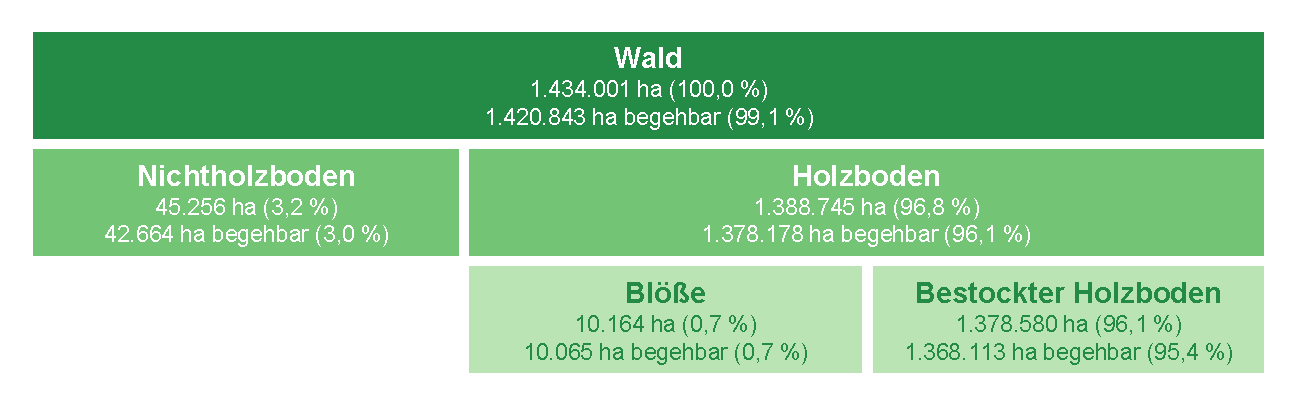
\includegraphics[width=\textwidth]{Grafiken/hzb/Abb_1_waldflaeche.pdf}
\caption{Waldkategorien in der Projektregion nach BWI-Definition \citep{ml_2014}. Dauerhaft unbestockte Waldfl�chen, wie Waldwege, Wildwiesen oder im Wald gelegene Moore, werden als Nichtholzboden bezeichnet. Bl��en sind vor�bergehend unbestockte Waldfl�chen.}
\label{fig:hzb:fig1_waldflaeche}
\end{figure}

Mit einer Waldfl�che von gut 1,4 Mio. ha liegt ca. 13 \% des deutschen Waldes \citep{ti_2014} in der untersuchten Projektregion (Abbildung \ref{fig:hzb:fig1_waldflaeche}). Der Bewaldungsanteil in der Projektregion betr�gt 31 \%. Dies entspricht in etwa dem Bundesdurchschnitt von 32 \% \citep{ti_2014}. Der Waldanteil ist jedoch regional unterschiedlich. Er liegt zwischen 17 \% im Westen Sachsen-Anhalts und 35 \% in S�dniedersachsen und Nordhessen.

Die W�lder der in weiten Teilen durch mesotrophe und eutrophe Lehmb�den gepr�gten Mittelgebirgslandschaft \citep{gauer_2012} zeichnen sich durch einen hohen Anteil von Laub- und Mischbest�nden aus. Mit 36 \% liegt der Laubwaldanteil deutlich �ber dem Nadelwaldanteil, welcher nur 14 \% betr�gt. Die H�lfte der Waldecken ist demnach mit Mischw�ldern bestockt. Lediglich 18 \% der Waldfl�che in der Region hat nur eine Baumart in der Hauptschicht. Ebenso zeichnen sich die W�lder der Region durch eine starke vertikale Differenzierung aus. Zwei Drittel der W�lder haben mindestens zwei Bestandesschichten.


\begin{figure}
\center
  \includegraphics[width=0.5\textwidth]{Grafiken/hzb/Abb_2_Buchenanteil.eps}
\caption{Buchenanteil an den BWI-Waldtrakten in der Projektregion. Die unterschiedlichen Punktgr��en ergeben sich aus den unterschiedlichen Traktabst�nden. Der Baumartenanteil bezieht sich auf den Hauptbestand, also die Bestandesschicht, auf der der wirtschaftliche Schwerpunkt liegt.}
\label{fig:hzb:fig2_buchenanteil}
\end{figure}


Im Rahmen der BWI wurden 86 Baumarten unterschieden. Um einen vertretbaren Sch�tzfehler und somit eine fundierte Aussage zu gew�hrleisten, wurden diese zu 8 Baumartengruppen (im Folgenden als Baumart bezeichnet) zusammengefasst. Wie aus Abbildung \ref{fig:hzb:fig2_buchenanteil} hervorgeht, ist die Rotbuche (\textit{Fagus sylvatica}) am Inventurzeitpunkt die am weitesten verbreitete Baumart in der Projektregion. Mit Ausnahme des Nordostens ist die Projektregion durch eine ganzfl�chige, homogene Buchenwaldverteilung ohne systematische Muster und ohne regionale Schwerpunkte charakterisiert. Mehr als jeder zweite Waldtrakt weist eine Buchenbeimischung von �ber 33 \% auf. Der Buchenanteil an der gesamten bestockten Holzbodenfl�che betr�gt 33 \%, was einer Fl�che von etwa 445.000 ha entspricht. Des Weiteren sind die Baumarten Fichte (\textit{Picea spec.} inkl. \textit{Abies spec.}, 22 \%), Eiche (\textit{Quercus robur}, \textit{Quercus petraea} und \textit{Quercus rubra}, 12 \%) und Kiefer (\textit{Pinus spec.}, 7 \%) in gr��eren Anteilen in der Projektregion vertreten. Andere Laubbaumarten mit hoher Produktionszeit (ALh), zu denen u. a. Ahorn (\textit{Acer spec.}) und Esche (\textit{Fraxinus excelsior}) z�hlen, sowie andere Laubbaumarten mit niedriger Produktionszeit (ALn), zu denen u. a. Birke (\textit{Betula spec.}) und Pappel (\textit{Populus spec.}) gerechnet werden, sind jeweils mit etwa 10 \% Fl�chenanteil vertreten. L�rche (\textit{Larix spec.}) und Douglasie (\textit{Pseudotsuga menziesii}) spielen demgegen�ber eine untergeordnete Rolle. Die Baumartenzusammensetzung findet sich in dieser Form in allen Eigentumsarten.

Das Mischungsverh�ltnis der Baumarten hat sich seit 2002 zugunsten der Laubbaumarten ver�ndert. Im Vergleich zur BWI 2 ist die Laubwaldfl�che bis 2012 um 52.000 ha angestiegen. Dem Anstieg der Laubwaldfl�che steht ein deutlicher R�ckgang der Nadelwaldfl�che von etwa 40.000 ha gegen�ber. Verantwortlich hierf�r ist der Fl�chenverlust der Fichte in H�he von etwa 35.000 ha und der Kiefer in H�he von etwa 10.000 ha. Fl�chenzunahmen (ca. 5.000 ha) sind beim Nadelholz nur bei der Douglasie zu verzeichnen.

%%------------------%%
%% Alter des Waldes %%
%%------------------%%
\subsection{Alter des Waldes}
\label{subsec:hzb:Ergebnisse:Alter}
Im Altersaufbau (Abbildung \ref{fig:hzb:fig3_altersklassen}) spiegelt sich die Nutzungsgeschichte und nat�rliche Entwicklung der W�lder in der Projektregion wider. Insbesondere gro�fl�chige Erst- und Wiederaufforstungen nach dem zweiten Weltkrieg sowie nach dem Orkan 1972 pr�gen die Altersklassenstruktur im Nadelwald, da f�r die Wiederbepflanzung der Freifl�chen zu der Zeit �berwiegend Nadelbaumarten verwendet wurden \citep{hmuklv_2014, ml_2014}. Aufgrund dessen ist mehr als die H�lfte des Nadelwaldes j�nger als 60 Jahre. In den Altersklassen 20 bis 60 Jahre dominieren die Nadelbaumarten, w�hrend in der Altersklasse 1 bis 20 Jahre sowie dem Jungwuchs unter Schirm die Laubbaumarten deutlich �berwiegen. Die Laubbaumanreicherung in den Jungbest�nden spiegelt das Umdenken im waldbaulichen Handeln Anfang der 1990er-Jahre nach den Erfahrungen des \textit{Waldsterbens} wider. Sie wurde relativ schnell fl�chenwirksam, weil die Orkane im ersten Jahrzehnt der 2000er-Jahre vor allem im S�den der Projektregion zu gr��eren Fl�chenverlusten im Nadelholz f�hrten, die h�ufig mit Laubbaumarten wieder aufgeforstet wurden \citep{hmuklv_2014}. Unter Ber�cksichtigung der Voranbauten unter Schirm weisen die Laubbaumarten Buche und Eiche einen sehr ausgeglichenen Altersklassenaufbau auf. Diese Verj�ngungsfl�che unter Schirm muss f�r eine vollst�ndige Darstellung der Ausgangssituation unbedingt mit ber�cksichtigt werden. Da in diesen F�llen zwei Bestandesschichten auf gleicher Fl�che stocken, werden die Jungwuchsbest�nde unter Schirm als �berschie�ende Fl�chen bezeichnet, welche nicht zum Hauptbestand z�hlen und somit nicht in die Berechnung der bestockten Waldfl�che eingehen. Andernfalls w�rde die tats�chliche Waldfl�che um die Fl�che des Jungwuchses �bersch�tzt werden.

\begin{figure}
\center
  \includegraphics[width=0.5\textwidth]{Grafiken/hzb/Abb_3_Altersklassen.eps}
\caption{Bestockte Holzbodenfl�che nach Altersklasse und Baumartengruppe in der Projektregion. Bei der Jungwuchsfl�che unter Schirm wurde kein Baumalter erhoben. Sie wird per Definition der ersten Altersklasse zugeordnet.}
\label{fig:hzb:fig3_altersklassen}
\end{figure}

%%--------------%%
%% Waldeigentum %%
%%--------------%%
\subsection{Waldeigentum}
\label{subsec:hzb:Ergebnisse:Waldeigentum}
Mit einem Fl�chenanteil von jeweils 35 \% an der Waldfl�che dominieren Privat- (inkl. privatrechtlicher Organisationen) und Landeswald vor dem K�rperschaftswald (24 \%), also Wald im Eigentum von St�dten oder Gemeinden sowie K�rperschaften, Anstalten oder Stiftungen �ffentlichen Rechts. Bundes- und Treuhandwald spielen eine untergeordnete Rolle. Wald im Landesbesitz, der von Anstalten oder K�rperschaften �ffentlichen Rechts bewirtschaftet wird, ist als Landeswald definiert. Die Betriebsgr��e ist ein wichtiges Strukturmerkmal zur n�heren Beschreibung des Privatwaldes, da sie Hinweise auf Organisationsgrad und Leistungsf�higkeit eines Forstbetriebes gibt. Etwa ein Drittel der Privatwaldfl�che, also ca. 11 \% der Gesamtwaldfl�che, ist kleinen Privatforstbetrieben mit einer Betriebsgr��e unter 20 ha Betriebsfl�che zuzuordnen. Demgegen�ber entfallen 60 \% des Privatwaldes auf gr��ere Forstbetriebe �ber 100 ha. Im Vergleich zum Bundesschnitt \citep{ti_2014} sind die Privatforstbetriebe der Projektregion damit tendenziell gr��er. In der r�umlichen Verteilung der 3 Haupteigentumsarten sowie der Gr��enklassen im Privatwald bestehen keine regionalen Unterschiede. Jede Eigentumsart und jede Gr��enklasse im Privatwald ist n�herungsweise homogen in der gesamten Projektregion vertreten.

%%----------------------------------------------%%
%% Nachhaltiges, kontinuierliches Holzpotenzial %%
%%----------------------------------------------%%
\subsection{Nachhaltiges, kontinuierliches Holzpotenzial}
\label{subsec:hzb:Ergebnisse:Nachhaltig}
Nach \citet{speidel_1972} ist die nachhaltige Forstwirtschaft als "F�higkeit eines Forstbetriebes, kontinuierlich und optimal Holznutzungen, Infrastrukturleistungen und sonstige G�ter zum Nutzen der gegenw�rtigen und zuk�nftigen Generationen hervorzubringen" definiert. W�hrend sich die Eingriffe in den j�ngeren Altersklassen auf die Pflege der Best�nde beschr�nken, die Zuw�chse nur teilweise abgesch�pft und die Holzvorr�te dementsprechend aufgebaut werden, f�hren die Hauptnutzungen in den �lteren Altersklassen zu einem mehr oder weniger schnellen Vorratsabbau, um die h�herwertigen Stammholzsortimente zu nutzen und die Verj�ngung einzuleiten bzw. um �ber der neuen Waldgeneration den Altholzschirm schrittweise zu r�umen. Dieses Nutzungsverhalten spiegelt sich in den zwischen BWI 2 und BWI 3 beobachteten Relationen von Holznutzung zu Holzzuwachs bei der Buche wider (Abbildung \ref{fig:hzb:fig4_zuw_nutz}). W�hrend der Holzzuwachs die Nutzung bis zu einem Bestandesalter von 120 Jahren �bersteigt, �berwiegt die Nutzung ab 140 Jahren deutlich.


\begin{figure}
\center
  \includegraphics[width=0.8\textwidth]{Grafiken/hzb/Abb_4_Zuwachs_Nutzung_nach_Baumalter.eps}
\caption{Durchschnittlicher j�hrlicher Vorratszuwachs und durchschnittliche j�hrliche Holznutzung der Buche nach Altersklasse in der gesamten Projektregion f�r den Zeitraum 2002 bis 2012. Die Holznutzung beinhaltet sowohl gewerbliche als auch private Nutzungen.}
\label{fig:hzb:fig4_zuw_nutz}
\end{figure}


Durch das multifunktionale Nachhaltigkeitsverst�ndnis der deutschen Forstbetriebe, wie es auch in den Waldgesetzen verankert ist, werden auf derselben Fl�che grunds�tzlich Nutz-, Schutz- und Erholungsfunktionen gleichzeitig, aber mit lokal unterschiedlicher Gewichtung verfolgt \citep{moller_2007}. Dieser integrative Ansatz erfordert, die Wechselwirkungen zwischen Nutzungs- und Naturschutzaspekten fl�chendeckend abzuw�gen und in Einklang zu bringen. In der Projektregion unterliegen ann�hernd 75 \% der Waldfl�che mehr oder weniger restriktiven Schutzgebietsauflagen (Abbildung \ref{fig:hzb:fig5_schutzgebiet}). Davon sind ca. 10.000 ha der strengsten Schutzkategorie Nationalpark zuzuordnen, wobei die BWI nicht zwischen Kernzonen ohne Nutzung und Entwicklungszonen mit Nutzung unterscheidet. Die Nutzung ist demnach nicht auf der gesamten Fl�che ausgeschlossen, jedoch zumindest sehr stark eingeschr�nkt. Ein Drittel der Waldfl�che unterliegt hohen Schutzgebietsauflagen. In diese Kategorie fallen Biosph�renreservate, Naturschutzgebiete und Natura 2000-Fl�chen. Auf diesen Fl�chen kann je nach Schutzgebietsart mit einer verminderten Holznutzung gerechnet werden. Ein Nutzungsausschluss ist jedoch in der Regel nicht zu erwarten. Hinzu kommen 560.000 ha auf denen Erholung, Erhaltung des Landschaftsbildes oder Wasserschutz im Vordergrund stehen. Auf diesen Fl�chen ist nicht von Nutzungseinschr�nkungen aufgrund des Schutzstatus auszugehen, es muss jedoch teilweise mit erschwerten Erntebedingungen gerechnet werden.


\begin{figure}
\center
  \includegraphics[width=0.9\textwidth]{Grafiken/hzb/Abb_5_Schutzgebietsauflagen.eps}
\caption{Schutzgebietsauflagen der Waldfl�chen in der Projektregion.}
\label{fig:hzb:fig5_schutzgebiet}
\end{figure}


Unter Ber�cksichtigung der Schutzgebietskulisse sowie der Altersausstattung des Waldes in der Projektregion betrug der j�hrliche Holzzuwachs der Buche nach BWI-Be"-rech"-nung"-en in der Periode 2002 bis 2012 durchschnittlich 3,9 Mio. Vfm Jahr$^{-1}$. Demgegen�ber stand die durchschnittliche j�hrliche Nutzung, welche ebenfalls �ber die BWI-Daten berechnet werden konnte, von 3,8 Mio. Vfm Jahr$^{-1}$. Trotz des rechnerischen Abzugs des nicht-nutzbaren Holzzuwachses vom Gesamt"-zuwachs lag der Zuwachs in der Bilanz der 10-j�hrigen Periode von 2002 bis 2012 noch leicht �ber der Nutzung. Der Gesamtzuwachs inkl. aller Altersklassen und Schutzgebietskategorien betrug 4,8 Mio. Vfm Jahr$^{-1}$. Das durchschnittlich genutzte Holzvolumen von 3,8 Mio. Vfm Jahr$^{-1}$ entspricht, nach Abzug von Rinde und Ernter�ckst�nden, einem Rohholzvolumen von 3,5 Mio. Efm Jahr$^{-1}$. Dieses l�sst sich mit BWI Daten nicht nach Sortimenten f�r bestimmte Holzverwendungen aufschl�sseln. Aus diesem Grunde fand im Rahmen des Projektes eine Befragung und Einsch�tzung des Einschnitts der wichtigsten buchenholzverarbeitenden Betriebe statt, die ihr Rohholz aus der Projektregion beziehen. Dar�ber hinaus wurden die Exportmengen eingesch�tzt. Die Analyse zeigte, dass durch die buchenholzverarbeitenden Betriebe sowie den nationalen und  internationalen Holzexport j�hrlich ca. 1 Mio. Efm Jahr$^{-1}$ Stammholz (inkl. Palettenholz) und 1 Mio. Efm Jahr$^{-1}$ Industrieholz aus der Projektregion aufgenommen wurden. Dies entsprach etwa 60 \% der tats�chlichen j�hrlich eingeschlagenen Rohholzmenge. Es ist davon auszugehen, dass die restlichen 1,5 Mio. Efm Jahr$^{-1}$ nahezu komplett energetisch verwendet wurden. Diese Einsch�tzung deckt sich in etwa mit den Ergebnissen einer Umfrage von knapp 10.000 Haushalten in ganz Deutschland durch die Universit�t Hamburg \citep{mantau_2012}, wonach deutschlandweit im Jahr 2010 knapp ein Drittel des Waldlaubholzaufkommens im Durchschnitt direkt energetisch genutzt wurde.

%%-----------------------------------------------------------%%
%% Entwicklung des Rohholzvorrates und des Rohholzpotenzials %%
%%-----------------------------------------------------------%%
\subsection{Entwicklung des Rohholzvorrates und des Rohholzpotenzials}
\label{subsec:hzb:Ergebnisse:Entwicklung}
Im Folgenden wird nicht nur das Rohholzpotenzial, sondern auch die prognostizierte Waldentwicklung in Vorratsfestemetern angegeben. Dies hat gegen�ber einer reinen fl�chigen Betrachtung den Vorteil, dass B�ume aller Bestandesschichten ber�cksichtigt sind und sich keine rechnerischen Schwierigkeiten durch �berschie�ende Fl�chen ergeben. Ferner bewirkt jeder Vorratsaufbau und -abbau auch eine Ver�nderung der Bestandesdichte und somit des Gesamtvorrates. Bei einer fl�chigen Betrachtung w�ren Ver�nderungen der Bestandesdichte nicht ersichtlich. Der Gesamtholzvorrat der Projektregion ist demnach eine abstrakte Kennzahl, aus welcher sich wesentliche R�ckschl�sse auf Produktivit�t, nachhaltige Nutzungsm�glichkeiten und die wirtschaftliche Leistungsf�higkeit der Forstbetriebe in der Projektregion ableiten lassen. Die Vorratsberechnungen 2002 und 2012 basieren auf BWI Daten, die Vorratsprognosen ab 2022 auf Waldentwicklungssimulationen.

Zwischen 2002 bis 2012 nahm der Buchenvorrat in allen L�ndern der Projektregion um insgesamt ca. 13 Mio. Vfm zu. Der Vorratsaufbau war im Landeswald st�rker ausgepr�gt als im Privat- und K�rperschaftswald. Im Vergleich der Baumarten Fichte und Kiefer ergab sich ein inhomogenes Bild. In Niedersachsen und Th�ringen gab es, bedingt durch den j�ngeren Altersaufbau, einen Vorratsaufbau, in Hessen und Nordrhein-Westfalen einen etwa gleichstarken Vorratsabbau. Obwohl es nennenswerte Fl�chenverluste bei diesen Baumarten gab (siehe Kapitel Waldfl�che), blieb der Vorrat der Fichte und Kiefer zwischen 2002 und 2012 aufgrund des hohen Fl�chenanteils der zuwachsstarken Altersklassen unver�ndert.

Die Simulationsergebnisse (Abbildung \ref{fig:hzb:fig6_prognose_vorrat_aus}) lassen einen kontinuierlichen Anstieg des Gesamtvorrates bei der Buche erwarten. Er ist im Jahr 2042 unter der Annahme unver�nderter waldbaulicher Vorgaben voraussichtlich etwa 25 \% h�her als 2002. W�hrend die Vorr�te der Eiche und der ALn stagnieren, steigt der Vorrat bei den ALh stetig an. Der Gesamtvorrat von Fichte und Kiefer nimmt bis einschlie�lich 2022 leicht ab. Ab 2022 w�chst ein Gro�teil dieser Nadelholzbest�nde in die Hiebsreife und der Vorrat nimmt ab diesem Zeitpunkt bis zum Ende der Simulation stetig ab. Bis zum Jahr 2042 wird der Holzvorrat der Fichten- und Kiefernbest�nde voraussichtlich um jeweils ein Drittel zur�ckgehen. Trotz einer Verdreifachung ihres Vorrates spielt die von einem niedrigen Ausgangsvorrat kommende Douglasie auch 2042 weiterhin nur eine untergeordnete Rolle in der Projektregion. Dieser Vorratszuwachs ist fast ausschlie�lich durch den hohen Zuwachs der bereits etablierten, zum Start der Simulation �berwiegend jungen Best�nde begr�ndet. Die L�rche spielt ebenfalls nur eine untergeordnete Rolle in der Region. Ihr Vorrat stagniert auf einem relativ niedrigen Niveau. Der Gesamtholzvorrat wird in den kommenden Jahren voraussichtlich zun�chst stagnieren und ab 2032 leicht sinken.


\begin{figure}
\center
  \includegraphics[width=0.5\textwidth]{Grafiken/hzb/Abb_6_Prognose_Vorrat.eps}
\caption{Entwicklung des Gesamtvorrates nach Baumartengruppe in der Projektregion. Die Gesamtvorr�te der Jahre 2002 und 2012 wurden aus den BWI Daten berechnet. Die Vorr�te ab 2022 wurden mit der Waldwachstumssimulationssoftware \textit{WaldPlaner} prognostiziert.}
\label{fig:hzb:fig6_prognose_vorrat}
\end{figure}


Der laufende j�hrliche Holzzuwachs je ha der Fichte liegt im bundesdeutschen Durchschnitt �ber alle Altersklassen etwa 50 \% �ber dem laufenden j�hrlichen Zuwachs der Buche \citep{ti_2014}. Die Waldumwandlung von Fichten- in Buchen- und in Mischbest�nde wird demnach nicht nur zu einer Verringerung der durchschnittlichen Bevorratung in der Projektregion f�hren, sondern langfristig auch das Zuwachsniveau und somit das Rohholzpotenzial insgesamt senken. Das voraussichtliche Nutzungspotenzial der Buche stagniert zun�chst bis 2031 auf einem Niveau von ca. 4 Mio. Vfm und steigt danach auf 4,8 Mio. Vfm an. Der Vorratsabbau in den vorratsreichen Nadelholzaltbest�nden wird im Simulationszeitraum zu einer Erh�hung des Fichten Rohholzaufkommens f�hren. Hierbei wird vor allem hiebsreifes Stammholz aus den Endnutzungen anfallen.

Das gesamte Nutzungspotenzial in der Projektregion steigt deshalb in der Simulationsperiode stetig um etwa 3 \% je Jahrzehnt an. Hierbei werden neben unver�nderten waldbaulichen Konzepten auch das Ausbleiben von Gro�schadereignissen oder Ausweitungen der Schutzgebietskulisse unterstellt.

%%%%%%%%%%%%%%%%%%%%%%%%%%%%%%%%%%%%%%%%%%%%%%%%%
%% Konsequenzen f�r die Nutzung von Buchenholz %%
%%%%%%%%%%%%%%%%%%%%%%%%%%%%%%%%%%%%%%%%%%%%%%%%%
\section{Konsequenzen f�r die Nutzung von Buchenholz}
\label{sec:hzb:Konsequenzen}
In der vorgestellten Projektregion hat die Laubholzwirtschaft eine gro�e Bedeutung. Das Buchenrohholzpotenzial ist nicht nur hoch, sondern aufgrund des hohen Buchenwaldanteils (Abbildung \ref{fig:hzb:fig2_buchenanteil}) und dessen relativ ausgeglichenen Altersklassenaufbaus (Abbildung \ref{fig:hzb:fig3_altersklassen}) gut sortiert. Ohne lange Transportwege sind alle holzwirtschaftlich relevanten Rohholzdimensionen verf�gbar.


\begin{figure}
\center
  \includegraphics[width=0.5\textwidth]{Grafiken/hzb/Abb_7_Prognose_aus_Bestand.eps}
\caption{Simulierte Entwicklung des Rohholzeinschlags nach Baumartengruppe in der Projektregion. Die Vorr�te wurden mit der Waldwachstumssimulationssoftware \textit{WaldPlaner} prognostiziert.}
\label{fig:hzb:fig6_prognose_vorrat_aus}
\end{figure}


Da die Wertsch�pfung beim Stammholz am h�chsten ist, zielt die Buchenwirtschaft auf eine m�glichst hohe Stammholzausbeute ab \citep{nagel_2008}. Dieses Stammholzpotenzial steht in den vorratsreichen Altholzbest�nden der Projektregion zur Verf�gung und ein nachhaltiger Nachschub ist durch die ausreichenden Fl�chen der mittleren Altersklassen zwischen 81 und 100 Jahren auch in Zukunft sichergestellt. Des Weiteren ist das Potenzial der schw�cheren Holzsortimente, insbesondere bei der Buche, nicht zu untersch�tzen. Industrieholz als Koppelprodukt der Stammholzernte und als Vornutzungsmaterial aus den j�ngeren Best�nden unter 80 Jahren gew�hrleistet die Rohstoffversorgung der Zellstoff- und Holzwerkstoffindustrie sowie der Heizkraftwerke und des Hausbrandes mit schw�cher dimensionierten Sortimenten. Die homogene r�umliche Verteilung der Eigentumsarten mit relativ gro�en Privatwaldbetrieben l�sst auf eine effektive Laubrohholzbereitstellung mit geringen regionalen Unterschieden schlie�en. Nicht zuletzt aus diesem Grund sind auch viele der deutschen Laubholzs�gewerke in dieser laubbaumreichen Region konzentriert \citep{ochs_2007}.

Das um alters- und schutzstatusbedingte Nutzungseinschr�nkungen bereinigte, nachhaltig nutzbare Buchenrohholzpotenzial der Projektregion wurde zwischen 2002 und 2012 fast komplett genutzt, wobei knapp drei Viertel der anfallenden Menge von der S�ge- und Holzwerkstoffindustrie aufgenommen wurde. Die Unternehmen der Holzindustrie nutzen den zur Verf�gung stehenden Holzzuwachs im Laubholz demnach zurzeit sehr effektiv. Gr��ere zus�tzliche Nutzungspotenziale lassen sich bei der Buche kurzfristig allenfalls durch eine Intensivierung der Holznutzung in den Best�nden �ber 140 Jahren erschlie�en. In diesen Altholzbest�nden ist oft kein weiterer Anstieg der Wertsch�pfung zu erwarten. Jedoch muss gerade in diesen Altholzbest�nden ber�cksichtigt werden, dass die Verj�ngung der n�chsten Waldgeneration sichergestellt ist und dass naturschutzfachliche Aspekte beachtet werden. Weitere Nutzungspotenziale f�r die Holzwerkstoff- und ggf. die Chemieindustrie liegen im Energieholzbereich. Wenn die Wertsch�pfungskette einen konkurrenzf�higen Holzpreis oberhalb des lokal sehr unterschiedlichen Energieholzpreises erlaubt, k�nnten Teile des bisher direkt energetisch genutzten Holzvolumens einer h�herwertigeren Verwendung zugef�hrt werden und je nach Nutzungsform durch Kaskadennutzung teilweise am Ende der Produktlebensdauer energetisch verwendet werden \citep{ruther_2007}. Die angespannte Konkurrenzsituation beim Buchenindustrieholz, welche sich durch die hohe Nachfrage nach Holz als Energietr�ger \citep{mantau_2012} und der Etablierung neuer Gesch�ftsfelder, wie der Bio�konomie \citep{mccormick_2013}, begr�ndet, spiegelt sich in der Verdopplung des j�hrlich durchschnittlichen Buchenindustrieholzpreises in Deutschland seit 2005 wider \citep{destatis_2016}. Aufgrund dieses stetigen Anstiegs setzen die Industrieholzverbraucher in der Projektregion immer st�rker auf internationalen Holzimport und Altholzankauf. Der milde Winter, die Verf�gbarkeit von Landschaftspflegeholz und die niedrigen �l- und Gaspreise f�hren aktuell zu einer Verringerung der Nachfrage nach Industrieholz als Energietr�ger. Zurzeit ist neben einer Entspannung auch ein �berhang an heimischem Buchenindustrieholz zu beobachten. Dieses spiegelt sich jedoch noch nicht im Jahresdurchschnitt der Holzpreisstatistiken wider.

Viele der erntereifen Kiefern- und Fichtenreinbest�nde werden im Simulationszeitraum voraussichtlich zu Laubbaum- oder Mischbest�nden �berf�hrt. Dieser Trend l�sst sich seit 2002 aus den BWI Daten ablesen \citep{fischer_2016} und wird voraussichtlich in der Simulationsperiode noch andauern \citep{ml_2004, bmel_2011}. Die prognostizierte Verschiebung des Vorrates hin zu mehr Laubbaumarten (Abbildung \ref{fig:hzb:fig6_prognose_vorrat_aus}) spiegelt also die Konsequenzen aus der aktuellen Waldpolitik wider. Da der Volumenzuwachs in Laubbaumbest�nden meist deutlich geringer als in Nadelbaumbest�nden ist, tragen die neubegr�ndeten Laub- und Mischw�lder im Durchschnitt weniger zum Vorratsaufbau bei als die reinen Nadelw�lder, aus denen sie hervorgegangen sind. In der Projektregion verl�uft der Vorratsaufbau der Buche deshalb langsamer als der Vorratsabbau der Fichte und Kiefer, was zur Stagnation und letztlich zur leichten Abnahme des gesamten Holzvorrates in der Projektregion f�hren wird.

Da sich die Struktur des Holzmarkts in der Vergangenheit stetig ver�ndert hat \citep{ochs_2007} und durch die Etablierung neuer Gesch�ftsfelder auch aktuell im Wandel ist \citep{mccormick_2013}, gestalten sich Prognosen �ber die Zukunft des Holzmarktes sehr schwierig. Aus diesem Grunde wurden keine Annahmen zur Entwicklung der Holznachfragemenge getroffen. Aus den Auswertungen wurde lediglich klar, dass das Holzpotenzial zwischen 2002 und 2012 weitestgehend ausgesch�pft wurde. Durch die mittelfristige Erh�hung des Nadelholzangebots wird sich das Gesamtrohholzpotenzial zun�chst erh�hen. Bedingt durch den fortschreitenden Umbau der Nadelholzbest�nde in Misch- oder Laubholzbest�nden folgt diesem voraussichtlichen mittelfristigen Anstieg jedoch ein stetiger R�ckgang des Rohholzangebotes. In der Projektregion Bei zuk�nftigen Investitionen oder F�rderma�nahmen muss deshalb unbedingt beachtet werden, dass die sich abzeichnende Erh�hung des gesamten Rohholzangebots nur eine zeitlich begrenzte Phase ist. Die Implementation zus�tzlicher Schutzgebiete w�rde das Rohholzpotenzial zus�tzlich reduzieren.

%%%%%%%%%%%%%%%%%%%%%%
%% Acknowledgements %%
%%%%%%%%%%%%%%%%%%%%%%
\section*{Danksagung}
\label{sec:hzb:Danksagung}
Dem Bundesministerium f�r Bildung und Forschung danken wir f�r die F�rderung des Projektes im Rahmen des Spitzenclusters \textit{BioEconomy}. Die Nutzung der BWI Daten wurde uns dankenswerterweise von den zust�ndigen Ministerien der L�nder Hessen, Niedersachsen, Nordrhein-Westfalen, Sachsen-Anhalt und Th�ringen bewilligt. F�r die Datenbereitstellung danken wir den Ministerien sowie dem Th�nen-Institut Eberswalde.
\end{otherlanguage}
	%\cleardoublepage
	\chapter{Biomass functions and nutrient contents of European beech, oak, sycamore maple and ash and their meaning for the biomass supply chain}
\label{chap:bm}
{\large Kai Husmann$^1$ - Sabine Rumpf$^2$ - J�rgen Nagel$^2$}\\

\vspace{3cm}
\noindent
$^1$University of G�ttingen, Department of Forest Economics and Forest Management,\\
B�sgenweg 3, 37077 G�ttingen, Germany \\

%\vspace{0.5cm}
\noindent
$^2$Northwest German Forest Research Institute, Department of Forest Growth, Section of Forest Growth Modeling and Computer Science,\\ Gr�tzelstra�e 2, 37079 G�ttingen, Germany\\

\vspace{\fill}
\noindent
Published in:\\
\textit{Journal of Cleaner Production} XXX (2017): X-Y\\
(DOI: 10.1016/j.jclepro.2017.03.019)

\newpage
\begin{itemize}
	\item Sabine Rumpf performed the nutrient efficiency analysis and coordinated the field work.
	\item J�rgen Nagel supported writing of the manuscript and the review process.
\end{itemize}

\clearpage
%%%%%%%%%%%%%%
%% Abstract %%
%%%%%%%%%%%%%%
\section*{Abstract}
\label{chap:bm:Abstract}
Woody biomass from forests has great potential to provide a continuous and largely carbon-neutral raw material supply for the bio-based industry. As the demand for forestry products is already very high and steadily increasing, the question arises how to match the limited available wood resources to the growing demand for raw materials. Thus, there is an initial need to properly estimate the available biomass from forests. The success of a bio-based industry depends on an accurate forecast of the raw material flow coming from the forests for the entire biomass supply chain up to the industrial processing stage. Using easily measured input data, e. g. the tree diameter at breast height, biomass functions allow for a reliable prediction of tree species- and tree fraction-specific single-tree biomasses. In combination with nutrient content data, the site specific ecologically sustainable level of forestry use can be assessed and the site-specific wood utilization potential can be fully exploited.

Biomass functions for the main tree species can be found in the literature. For other tree species, like sycamore or ash, however, there are only very specific studies available. As the wood potential of especially those species is recently often unused, goal of this study is to develop biomass functions and nutrient contents for European beech, oak, ash and sycamore for the fractions stem wood, bark, branches, and twigs.

For this purpose 139 trees were destructively sampled. Their single tree biomasses and nutrient contents were examined. This data was then used in a regression analysis to build generalized tree species- and tree fraction-specific biomass functions and nutrient contents for northern and central Germany.
We showed that the sycamore and ash biomass functions differed significantly from those of European beech and oak. Using oak biomass functions for the biomass estimation of sycamore and ash, as it is practiced today, leads to a massive overestimation of the standing biomass in a test site up to 11 \% (21 tons / ha respectively).

The share of species-rich broadleaf forest stands, and thereby the importance of tree specific biomass functions, is increasing. The introduced models can help to exploit the huge biomass potential of those deciduous stands.

\subsection*{Keywords}
Biomass function - Nutrient content - Long-living tree species - Biomass supply chain - Site sustainability

\subsection*{Highlights}
\begin{itemize}
\item Effectivity of biomass supply chains depend on reliable biomass estimation.
\item The wood potential of long-living tree species is recently often unused.
\item Biomass models for sycamore maple and ash can help gathering this potential.
\end{itemize}
%%%%%%%%%%%%%%%%%%
%% Introduction %%
%%%%%%%%%%%%%%%%%%
\section{Introduction}
\label{sec:bm:Introduction}

Biomass from forests has real potential to provide a continuous and largely carbon-neutral supply of material to the bio-based industry sector and can therefore make a significant contribution to a clean bio-based industry. Especially small dimensioned wood has huge potential for use in bio-refineries. \citet{ekman_2013} showed in Sweden that previously unused scrap wood can be used for the extraction of high quality chemical substances, such as bio-oils or antioxidants for use in the food or cosmetics industries. Supply of biomass from forestry can drive the economic growth of the entire bio-based chemical industry and make it competitive in the long-term, especially if wood fractions that have up to now been used as fuel wood are included. Innovative industries, such as the nanofiber or biochemistry industries, are increasing the demands on the forestry product-pool. The forest-based bio-economy is already an integral part of the global forestry sector \citep{hurmekoski_2013}. The European bio-based industry is currently a growing sector, with Germany playing a leading role \citep{hennig_2016}.

The global forestry industry is currently undergoing a process of change. The use of wood as raw materials in Germany has increased considerably in the last decades \citet{mantau_2012}. Changes in government energy policy and the development of new technology led to development of new markets, in particular for small dimensioned wood \citep{geldermann_2016, mccormick_2013}. The demand for forestry products is steadily rising, increasing the competition for raw timber. The question then is how to match the available wood resource to the demand for raw materials.

Just as it is for classical forestry \citep{mohring_1997}, knowledge of the available potential biomass is the main prerequisite for a functioning bio-based industry \citep{hennig_2016}. Using wood means that the nutrients bound in the wood are removed from the forest ecosystem. The biomass potential of a forest can only be utilized to an extent that, in the long-term, won�t deplete the supply of plant available nutrients in the forest ecosystem. In order to be able to exploit the woody biomass potential for the bio-based industry, the limit of the utilisation extend from the forests stands must be known \citep{block_2013, pretzsch_2014}. Therefore, reliable estimates of the quantity of biomass to be harvested, as well as reliable estimates of the amount of nutrients contained in these biomasses are required.

Using easily measured input data, such as diameter at breast height (dbh) or tree height, biomass functions enable the prediction of single-tree biomasses. Tree species and tree-fraction specific estimations of the forest biomass supply can be made. Using these biomass functions coupled with nutrient content data, the nutrient export can be estimated. In this way an ecologically sustainable level of forestry use can be calculated and the site specific wood utilization potential can be fully exploited.

The success of the bio-based industry depends to a great extent on the ability to accurately forecast the flow of raw materials in the integrated biomass supply chain \citep{geldermann_2016, how_2016}. Using biomass functions the relevant information for strategic operational decision-making can be generated for the entire biomass supply chain - from the forest stand to the industrial processing stage. Detailed biomass calculations can improve planning certainty along the entire value chain because the masses to be transported and those due at the factory gate can be forecasted very accurately. Biomass functions can therefore make an important contribution to increasing the planning capability, and thereby to cost reductions, in operative planning for forestry enterprises, wood logistics and wood industry firms.

Wood industry cluster studies on the availability of raw materials and on the market situation of the wood industry are the bases for the strategic orientation of the bio-economy industries \citep{mccormick_2013}. By using supply analyses and material flow simulations together with biomass functions decision support models can be parameterised which enable, for example, the computing of a continuous biomass supply chain (e.g. \citet{ruther_2007, wordehoff_2011, mantau_2012}).

Responsible biomass usage from forests has, next to its economic relevance, also very important social impacts. In 2006, under the terms of the Kyoto protocol, reporting of the carbon sequestration performance of forests became mandatory in Germany. The use of biomass functions is an integral part of this reporting process \citep{vallet_2006, tabacchi_2011, wordehoff_2011}.

In the literature there are numerous biomass functions (e.g. \citet{grote_2003, cienciala_2005, pretzsch_2014}) and nutrient content figures (e.g. \citep{augusto_2000, jacobsen_2003, weis_2012, pretzsch_2014}) available for the tree species European beech (\textit{Fagus sylvatica} [L.]), common oak (\textit{Quercus robur} [L.]) and sessile oak (\textit{Quercus petraea} [Matt.]). For sycamore maple (\textit{Acer pseudoplatanus} [L.]) and ash (\textit{Fraxinus excelsior} [L.]) however, there are only few functions available. All literature functions found either do not cover the entire relevant diameter spectrum (e.g. \citet{albert_2014, alberti_2005}) or do not allow fraction specific biomass estimation \citep{bunce_1968}.

The wood increment of long-term deciduous trees, which is the species group sycamore and ash belong to, was only used by 38 \% between 2002 and 2012 \citep{ti_2014}. This is certainly partially reasoned by the fact that reliable planning methods for long-term deciduous species are not available. The question then arises if the predictions of the woody biomass in these stands could be improved by using specific biomass functions and nutrient contents for sycamore and ash. Specific biomass functions for these species could help making the recently unused potential available for the bio-based industry.

The goal of this study is to develop biomass functions for European beech, oak, sycamore and ash by means of regression analysis, using data gathered in northern and central Germany. Functions are developed for the tree fractions stem wood (diameter > 7cm without bark), bark of stem wood, branches (1 - 7cm with bark), and twigs (< 1cm with bark). The differences in these biomass functions are examined at single-tree and stand level by means of a sensitivity analysis in an exemplary test stand. The nutrient content in the different tree fractions of the tree species studied are determined and used as the basis for quantifying the nutrient removal by harvesting. The amount of nutrients that are removed from the forest ecosystem is then determined by multiplying the nutrient content with the biomass.

%%%%%%%%%%%%%%%%%%%%%%%%%%%
%% Materials and Methods %%
%%%%%%%%%%%%%%%%%%%%%%%%%%%
\section{Materials and Methods}
\label{sec:bm:methods}
With the goal of quantifying biomass and nutrient content 139 vital trees were studied (Table \ref{tab:bm:tab1}). The sample plots for beech and oak represented as many different growing areas and site conditions as possible. The high nutrient requirements of sycamore and ash meant that the sample plots for these species were exclusively on nutrient-rich, calcareous substrates. Per plot 2 - 4 trees were chosen (Figure \ref{fig:bm:fig1}). Both within each sample site, and across the plots as a whole, the aim was to collect trees from a wide and evenly distributed diameter range.

\begin{figure}
	\center
	\includegraphics[width=0.7\textwidth]{Grafiken/bm/Fig_1_Locations.eps}
	\caption{Locations of the 54 sampled plots. Source of the background map: \citet{facg_2014}.}
	\label{fig:bm:fig1}
\end{figure}

% Please add the following required packages to your document preamble:
% \usepackage{multirow}
\begin{table}[]
	\centering
	\caption{Descriptive statistics of the sampled trees.}
	\label{tab:bm:tab1}
	\begin{tabular}{cccccc}
		\cline{1-6}
		\multicolumn{1}{l}{}    &                          & oak   & \begin{tabular}[c]{@{}c@{}}European\\ beech\end{tabular} & ash   & sycamore \\ \cline{1-6}
		\multicolumn{1}{l}{}    &     number of trees             & 40   & 37 & 37   & 25 \\ \cline{1-6}
		
		\multirow{4}{*}{dbh {[}cm{]}}    & minimum     & 8.00  & 8.00                                                    & 9.10  & 12.00    \\
		&  mean        & 35.40 & 32.50                                                   & 31.90 & 28.20    \\
		&  std. dev.   & 23.70 & 17.14                                                   & 17.30 & 10.40    \\
		&  maximum     & 95.40 & 66.40                                                   & 75.60 & 56.10    \\ \cline{1-6} 
		\multirow{4}{*}{height {[}m{]}} &  minimum   & 9.60  & 15.30                                                   & 14.40 & 15.20    \\
		&  mean      & 22.10 & 24.90                                                   & 25.60 & 22.60    \\
		& std. dev. & 6.90  & 6.65                                                    & 6.70  & 4.25     \\
		&  maximum   & 32.00 & 35.25                                                   & 38.50 & 31.80    \\ \cline{1-6} 
		\multirow{4}{*}{age {[}a{]}}    &  minimum      & 25    & 21                                                      & 34    & 33       \\
		&  mean         & 86    & 84                                                      & 74    & 51       \\
		&  std. dev.    & 54    & 44                                                      & 37    & 23       \\
		& maximum      & 190   & 180                                                     & 153   & 118      \\ \cline{1-6} 
	\end{tabular}
\end{table}
%%-------------------------------------%%
%% Data sampling and sample processing %%
%%-------------------------------------%%
\subsection{Data sampling and sample processing}
\label{subsec:bm:methods:sampling}

Dbh, height at crown base and tree height were measured for each tree. The fraction volumes of the trees were determined using randomized branch sampling (RBS). RBS is an efficient and bias free sampling method for estimating tree fractions \citep{saborowski_1999, Gregoire_2008}. Since this method was firstly described \citet{jessen_1955} it has been used in other studies, including those from \citet{valentine_1984}, \citet{gaffrey_1999} and \citet{affleck_2015}. This multi-stage sampling method assumes proportionality between the target quantity and an easily measurable proxy. Because an allometric relationship exists between branch volume and branch base diameter \citep{west_1999}, the RBS method makes it possible to estimate the wood volume by measuring only a subset of branch lengths and branch diameters in the tree crowns. The stem form was assessed by section-wise diameter measurements at certain tree heights up to the crown base. In order to determine the specific bulk density and nutrient contents, up to 12 samples, covering all diameters of the tree, were collected per tree using the Importance Sampling \citep{Gregoire_2008}.

Half of the samples were measured and weighted in fresh state and, after several days drying at 103 �C, in absolute dry condition in order to determine the bulk density [kg biomass (dry) / m$^3$ wood volume (fresh)] \citep{rademacher_2011}. For all stem wood samples (diameter > 7cm) the bark was separated from the wood before drying. From this samples tree species and tree fraction specific bulk density coefficients were calculated. The fraction volumes, which were previously estimated using the RBS method, could then be converted into biomasses using these bulk density coefficients. The other half of the samples underwent a chemical analysis in order to determine their nutrient concentrations. In our sample preparation and analysis we followed the widely used method by \citet{konig_2012a, konig_2012b}. In order to ensure comparability between all studied tree species, only European beech and oak samples from sample plots on nutrient-rich substrates were considered for the chemical analysis.

%%-------------------%%
%% Biomass functions %%
%%-------------------%%
\subsection{Biomass functions}
\label{subsec:bm:methods:bm_functions}

In order to parameterize tree species and tree fraction dependent biomass functions the single-tree biomass information was analyzed by regression analysis. The biomass functions were estimated using nonlinear Generalized Least Squares Estimation. The exponential function used in \citet{hochbichler_2006} (Equation \ref{eq:bm:eq1}) was chosen as the model type \citep{rumpf_2011}. The validity of each model was tested via visual analysis of the weighted model residuals including a comparison with theoretical residuals (quantile-quantile-analysis). Furthermore the bias of each model was calculated as the mean of the model residuals.

\begin{equation}
\label{eq:bm:eq1}
\hat{Y}_i=\exp{\left(\alpha+\beta \, ln(dbh_i)+\gamma \, ln(h_i)\right)}\,\varepsilon_i
\end{equation}

One general assumption in regression analysis is the independence of the model errors $\varepsilon_i$. Because this assumption is probably not met for the tree fractions within a tree species, a model distortion due to correlation between the covariates (collinearity) is possible. Not taking this collinearity into account can influence the results of a regression and thereby limit the model validity \citep{graham_2003}. In order to estimate the magnitude of the error resulting from collinearity, in addition to the single model variances $var(\hat{y}_i)$, combined model variances per tree species $\hat{\bar{y}}$ were calculated \citep{parresol_2001}. This combined model variance per tree species consists of the single model variances $var(\hat{y}_i)$ and the model co-variances $cov(\hat{y}_i, \hat{y}_j)$ between the fraction functions for a respective tree species (Equation \ref{eq:bm:eq2}). The correlation between two fractions  was estimated using a linear correlation coefficient of the measured biomasses.

\begin{equation}
\label{eq:bm:eq2}
\begin{aligned}
var\left(\operatorname{\hat{\bar{y}}\hspace{0.25em}}\right) &=\sum_{i=1}^c var\left(\operatorname{\hat{y}_i\hspace{0.25em}}\right)+2\sum_{i<j}\sum cov\left(\operatorname{\hat{y}_i\hspace{0.25em}}, \operatorname{\hat{y}_j\hspace{0.25em}}\right)\\
\text{Where}\hspace{0.25em}c&=\text{Number of biomass functions,}\\
cov\left(\operatorname{\hat{y}_i},\operatorname{\hat{y}_j}\right)&=\operatorname{\hat{\rho}}_{\operatorname{\hat{y}_i},\operatorname{\hat{y}_j}}\sqrt{var\left(\operatorname{\hat{y}_i\hspace{0.25em}}\right)\hspace{0.25em}var\left(\operatorname{\hat{y}_j\hspace{0.25em}}\right)},\\
\text{and}\hspace{0.25em}\operatorname{\hat{\rho}}_{\operatorname{\hat{y}_i},\operatorname{\hat{y}_j}}&=\text{estimated correlation between fractions $y_i$ and $y_j$.}
\end{aligned}
\end{equation}

The multiplicative error term $\varepsilon_i$ of the nonlinear biomass function (Equation \ref{eq:bm:eq2}) implies an increasing variance with increasing covariate dimension. We quantified the resulting heteroscedasticity by parameterizing a power function with the model residuals over the fitted values. This function was then used to weight the residuals of the actual fit. Thus, neither the variances of the distinct biomass functions $var(\hat{y}_i)$ nor the combined model variance $var(\hat{\bar{y}}_i)$ showed heteroscedasticity.

In order to make the single model variances $var(\hat{y}_i)$ comparable to each other, to the variances of other biomass functions in the literature and to the combined model variances per tree species $var(\hat{\bar{y}}_i)$, dimensionless coefficients of variation for each model $i$ were calculated (Equation \ref{eq:bm:eq3}), where $j$ is the index for the observed tree. These coefficients of variation were also calculated for the combined model error $v(\hat{\bar{y}}_i)$. $v(\hat{y}_i)$ and $v(\hat{\bar{y}}_i)$ thus represent the normalized deviation of the models. They are calculated as the quotient of the deviation and the estimated response. This normalization is advantageous since it scales every residuum by its expected dimension thereby making it easily interpretable and comparable. The absolute deviation would, due to the heteroscedasticity, increase with increasing dimension of the response $y_{ij}$.

\begin{equation}
\label{eq:bm:eq3}
v\left(\operatorname{\hat{y}_i}\right)=\frac{1}{N_i-1}\sqrt{
\sum_{j=1}^{N_i}\left(\frac{\operatorname{y_{ij}}-\operatorname{\hat{y}_{ij}}}{\operatorname{\hat{y}_{ij}}}\right)^2}
\end{equation}

where $i$ denotes the fraction and $j$ the observed tree. $N_i$ is the number of observations in fraction $i$. The entire regression analysis was performed using with the R package \textit{nlme} \citep{venables_2002}. Additionally, we calculated the likelihood-ratio based pseudo-r-squared for each model using \textit{MuMIn} \citep{barton_2016}.

To enable a comparison between the biomass functions for the different tree species 95 \% confidence intervals were computed for European beech and oak using bootstrapping \citep{diciccio_1996}. To do this every regression model for these two species was repeated 1,000 times using sub-samples of the original data which were selected randomly by drawing with replacement. In order to prevent the sample size influencing the width of the confidence intervals, the number of samples in every repetition matched the actual number of samples. All analyses were performed using the R software \citep{r_core_team_2016}.

%%----------------------%%
%% Sensitivity analysis %%
%%----------------------%%
\subsection{Sensitivity analysis}
\label{subsec:bm:methods:sensitivity}
To analyze the behavior of our models, the biomass functions were applied on a real forest site. This site was chosen for testing purposes only. The trees of the site were not included in the regression analyses. The research site is located ca. 15 km east of the city of G�ttingen. It is a mixed stand with European beech, sycamore and ash, which is typical for this region. The site is on a sun exposed slope with a stony substrate consisting of the products of limestone weathering overlain by a thin layer of loess (Table \ref{tab:bm:tab2}). It has a good nutrient and a good water supply.

\begin{table}[]
	\centering
	\caption{Tree layer specific parameters of the test site. Growth region: Middle German Trias High and Hill Land. Growth district: G�ttingen Forest. Altitude: 340 m. hm: Height of stem of mean basal area. dm: Diameter of stem of mean basal area.}
	\label{tab:bm:tab2}
	\begin{tabular}{ccccc}
		\hline
		tree species   & age & \begin{tabular}[c]{@{}c@{}}hm \\ {[}m{]}\end{tabular} & \begin{tabular}[c]{@{}c@{}}dm \\ {[}cm{]}\end{tabular} & \begin{tabular}[c]{@{}c@{}}stand volume \\ {[}m$^3$ ha$^{-1}${]}\end{tabular} \\ \hline
		European beech & 76  & 23.3                                                  & 27.6                                                   & 164.0                                                               \\
		European beech & 20  & 14.9                                                  & 11.2                                                   & 4.8                                                                 \\
		ash            & 71  & 28.7                                                  & 35.2                                                   & 73.3                                                                \\
		sycamore       & 76  & 24.3                                                  & 23.6                                                   & 18.7                                                                \\ \hline
	\end{tabular}
\end{table}

Based on this test site, 5 simulated test sites, differing in their species composition, were generated. For this, the proportions of the 3 tree species in the real stand were modified using the \textit{WaldPlaner} forest simulator \citep{hansen_2014}. With this software we randomly cloned original trees from the test site until the target mix ratio was achieved.
%%-------------------%%
%% Nutrient contents %%
%%-------------------%%
\subsection{Nutrient contents}
\label{subsec:bm:methods:nutrients}
To consider site sustainability is to ask the question - how to best manage the scarce nutrient resources available? To do this, the nutrient response efficiencies of the distinct species and fractions appear to be a reasonable \citep{henderson_2012}. The nutrient response efficiency \citep{vitousek_1982} tells us how much carbon [kg] can be bound by a plant per 1 kg of applied nutrients. According to \citet{vitousek_1982}, we define the response efficiency as the inverse of the element concentration of the biomass. It is the ratio of carbon to the other mineral nutrients. The tree and fraction specific nutrient response efficiency of each nutrient is thus calculated by dividing the carbon concentration by the respective nutrient concentration in the tree fractions. It determines how much nutrient must be assimilated to grow a certain amount of biomass. Trees with high nutrient response efficiency need less nutrients to grow the same amount of biomass in the respective fraction than a plant with lower nutrient response efficiency. The total tree nutrient response efficiency was calculated by dividing the total tree concentration of carbon, the sum of all 4 fractions, by the total concentration of the respective nutrient. From the samples that were chemically tested, the average nutrient response efficiencies per tree species and were calculated. This was achieved by calculating the mean nutrient response efficiencies per tree species from the single-tree values.

%%%%%%%%%%%%%
%% Results %%
%%%%%%%%%%%%%
\section{Results}
\label{sec:bm:results}

%%-------------------%%
%% Biomass functions %%
%%-------------------%%
\subsection{Biomass functions}
\label{subsec:bm:results:bm_functions}

The numbers of parameters in the biomass functions were determined by Akaike Information Criterion (AIC) \citet{akaike_1981}. By including tree height in the models for stem wood and bark the AIC scores were lowered markedly. This was observed for all species. In those cases, where tree height had a significant influence on the biomass, additional models were calculated with the dbh as the only independent variable. As a consequence of this, for each of the tree species there is an easily applicable dbh model available for each function. The coefficients of variation $v(\hat{\bar{y}}_i)$ and $v(\hat{y}_i)$ allowed a direct comparison of the single and the combined variances. In those cases in which the tree height coefficient was significant the model coefficients of variation were markedly reduced by its inclusion. The coefficients of variation fall into two groups (Table \ref{tab:bm:tab3}). The coefficients of variation for the functions of stem wood and bark of the stem wood are clearly smaller than those for branches and twigs. Even if the height is not included $v(\hat{y}_i)$ of the stem wood and bark models is substantially smaller than $v(\hat{y}_i)$ of the branches and twigs.

\begin{table}[]
	\centering
	\caption{Coefficients and standard deviation of the biomass functions (Equation \ref{eq:bm:eq1}) for the tree species European beech, oak, ash and sycamore including a combined model error (Equation \ref{eq:bm:eq2}) for each species. $v(\hat{y}_i)$: Coefficient of variation. $r^{2}_{LR}$: likelihood-ratio based pseudo-r-squared.}
	\label{tab:bm:tab3}
	\begin{tabular}{ccccccccc}
		\hline
		species  & N  & fraction          & $\alpha$             & $\beta$      & $\gamma$     & AIC   & $v(\hat{y}_i)$     & $r^{2}_{LR}$     \\ \hline
		oak      & 41 & \multicolumn{2}{c}{combined model error} &              &              &       & 0.040 &       \\ \hline
		&    & stem wood         & -5.6509              & 1.9222       & 1.6316       & 435.9 & 0.039 & 0.998 \\
		&    &                   & ($\pm$0.354)         & ($\pm$0.102) & ($\pm$0.211) &       &       &       \\
		&    & bark              & -6.3130              & 1.7037       & 1.5738       & 310.3 & 0.039 & 0.997 \\
		&    &                   & ($\pm$0.348)         & ($\pm$0.102) & ($\pm$0.209) &       &       &       \\ \cline{3-9} 
		&    & stem wood         & -2.8992              & 2.5924       &              & 468.2 & 0.050 & 0.997 \\
		&    &                   & ($\pm$0.205)         & ($\pm$0.057) &              &       &       &       \\
		&    & bark              & -3.6611              & 2.3505       &              & 340.7 & 0.049 & 0.995 \\
		&    &                   & ($\pm$0.201)         & ($\pm$0.056) &              &       &       &       \\
		&    & branch            & -1.3987              & 1.5827       &              & 377.1 & 0.131 & 0.975 \\
		&    &                   & ($\pm$0.332)         & ($\pm$0.114) &              &       &       &       \\
		&    & twig              & -3.1298              & 1.6758       &              & 307.9 & 0.201 & 0.891 \\
		&    &                   & ($\pm$0.657)         & ($\pm$0.201) &              &       &       &       \\ \hline
		beech    & 38 & \multicolumn{2}{c}{Combined model error} &              &              &       & 0.036 &       \\ \hline
		&    & stem wood         & -4.5238              & 2.1778       & 1.0373       & 414.5 & 0.037 & 0.996 \\
		&    &                   & ($\pm$0.393)         & ($\pm$0.088) & ($\pm$0.196) &       &       &       \\
		&    & bark              & -6.0328              & 1.9511       & 0.9515       & 221.1 & 0.035 & 0.995 \\
		&    &                   & ($\pm$0.362)         & ($\pm$0.080) & ($\pm$0.183) &       &       &       \\ \cline{3-9} 
		&    & stem wood         & -2.5687              & 2.5852       &              & 438.1 & 0.049 & 0.993 \\
		&    &                   & ($\pm$0.193)         & ($\pm$0.056) &              &       &       &       \\
		&    & bark              & -4.2350              & 2.3230       &              & 242.2 & 0.043 & 0.992 \\
		&    &                   & ($\pm$0.175)         & ($\pm$0.051) &              &       &       &       \\
		&    & branch            & -1.1673              & 1.5580       &              & 349.5 & 0.117 & 0.897 \\
		&    &                   & ($\pm$0.340)         & ($\pm$0.110) &              &       &       &       \\
		&    & twig              & -3.4372              & 1.6993       &              & 282.5 & 0.283 & 0.802 \\
		&    &                   & ($\pm$0.839)         & ($\pm$0.271) &              &       &       &       \\ \hline
		ash      & 37 & \multicolumn{2}{c}{Combined model error} &              &              &       & 0.026 &       \\ \hline
		&    & stem wood         & -4.3728              & 1.9730       & 1.1765       & 374.2 & 0.023 & 0.999 \\
		&    &                   & ($\pm$0.157)         & ($\pm$0.050) & ($\pm$0.092) &       &       &       \\
		&    & bark              & -6.8483              & 1.9737       & 1.2909       & 256.8 & 0.032 & 0.997 \\
		&    &                   & ($\pm$0.341)         & ($\pm$0.092) & ($\pm$0.180) &       &       &       \\ \cline{3-9} 
		&    & stem wood         & -2.4182              & 2.5144       &              & 426.9 & 0.039 & 0.996 \\
		&    &                   & ($\pm$0.189)         & ($\pm$0.053) &              &       &       &       \\
		&    & bark              & -4.3601              & 2.4730       &              & 289.4 & 0.045 & 0.994 \\
		&    &                   & ($\pm$0.237)         & ($\pm$0.064) &              &       &       &       \\
		&    & branch            & -2.1015              & 1.8858       &              & 330.7 & 0.074 & 0.969 \\
		&    &                   & ($\pm$0.286)         & ($\pm$0.087) &              &       &       &       \\
		&    & twig              & -3.3426              & 1.6436       &              & 242.0 & 0.174 & 0.857 \\
		&    &                   & ($\pm$0.657)         & ($\pm$0.204) &              &       &       &       \\ \hline
		\multicolumn{9}{l}{Continued on next page}
	\end{tabular}
\end{table}

\begin{table*}[]
	\centering
	%%\caption*{Table \ref{tab:bm:tab3} (continued)}
	\begin{tabular}{ccccccccc}
		\hline
		species  & N  & fraction          & $\alpha$             & $\beta$      & $\gamma$     & AIC   & $v(\hat{y}_i)$     & $r^{2}_{LR}$     \\\hline
		sycamore & 25 & \multicolumn{2}{c}{Combined model error} &              &              &       & 0.039 &       \\ \hline
		&    & stem wood         & -4.1220              & 2.0364       & 0.9797       & 225.1 & 0.029 & 0.997 \\
		&    &                   & ($\pm$0.274)         & ($\pm$0.082) & ($\pm$0.163) &       &       &       \\
		&    & bark              & -5.8308              & 1.8880       & 0.9918       & 118.2 & 0.030 & 0.996 \\
		&    &                   & ($\pm$0.274)         & ($\pm$0.083) & ($\pm$0.165) &       &       &       \\ \cline{3-9} 
		&    & stem wood         & -2.4235              & 2.4461       &              & 249.5 & 0.046 & 0.992 \\
		&    &                   & ($\pm$0.215)         & ($\pm$0.064) &              &       &       &       \\
		&    & bark              & -4.1984              & 2.3299       &              & 141.9 & 0.047 & 0.991 \\
		&    &                   & ($\pm$0.212)         & ($\pm$0.064) &              &       &       &       \\
		&    & branch            & -3.5005              & 2.1777       &              & 211.7 & 0.160 & 0.916 \\
		&    &                   & ($\pm$0.593)         & ($\pm$0.190) &              &       &       &       \\
		&    & twig              & -5.6275              & 2.3005       &              & 147.9 & 0.252 & 0.893 \\
		&    &                   & ($\pm$0.932)         & ($\pm$0.298) &              &       &       &       \\ \hline
		
\end{tabular}
\end{table*}

Altogether $v(\hat{y}_i)$ ranged from 0.02 to 0.28. With values between 0.03 and 0.04, the combined model coefficients of variation when collinearity is taken into account (Equation \ref{eq:bm:eq2}) were always small. The combined $v(\hat{\bar{y}}_i)$ were calculated from the respective best models (the models with height parameter for stem wood and bark). The combined model coefficients for the European beech, oak and ash models were very close to the coefficients for stem wood and stem wood bark. Although there were correlations between fractions, these were higher for models with low variance. Accordingly the combined model coefficients of variation for European beech, oak and ash were low. Only the sycamore model showed considerable difference between the combined model variation coefficients and the variation coefficients of stem wood and bark of the stem wood. This is explained by the relatively high correlation between the stem wood biomass with the branch and twig biomasses. Despite this, because the coefficients of variation for the sycamore stem wood and bark models are relatively low, the combined model coefficients of variation are approximately the same as those for European beech and oak. As the residuals of each model as well as all biases were not trending and each bias was near 0, it can be assumed that all models are valid. The highest relative bias found amounted only 1.8 \% of the mean expectation.

\begin{figure}
	\center
	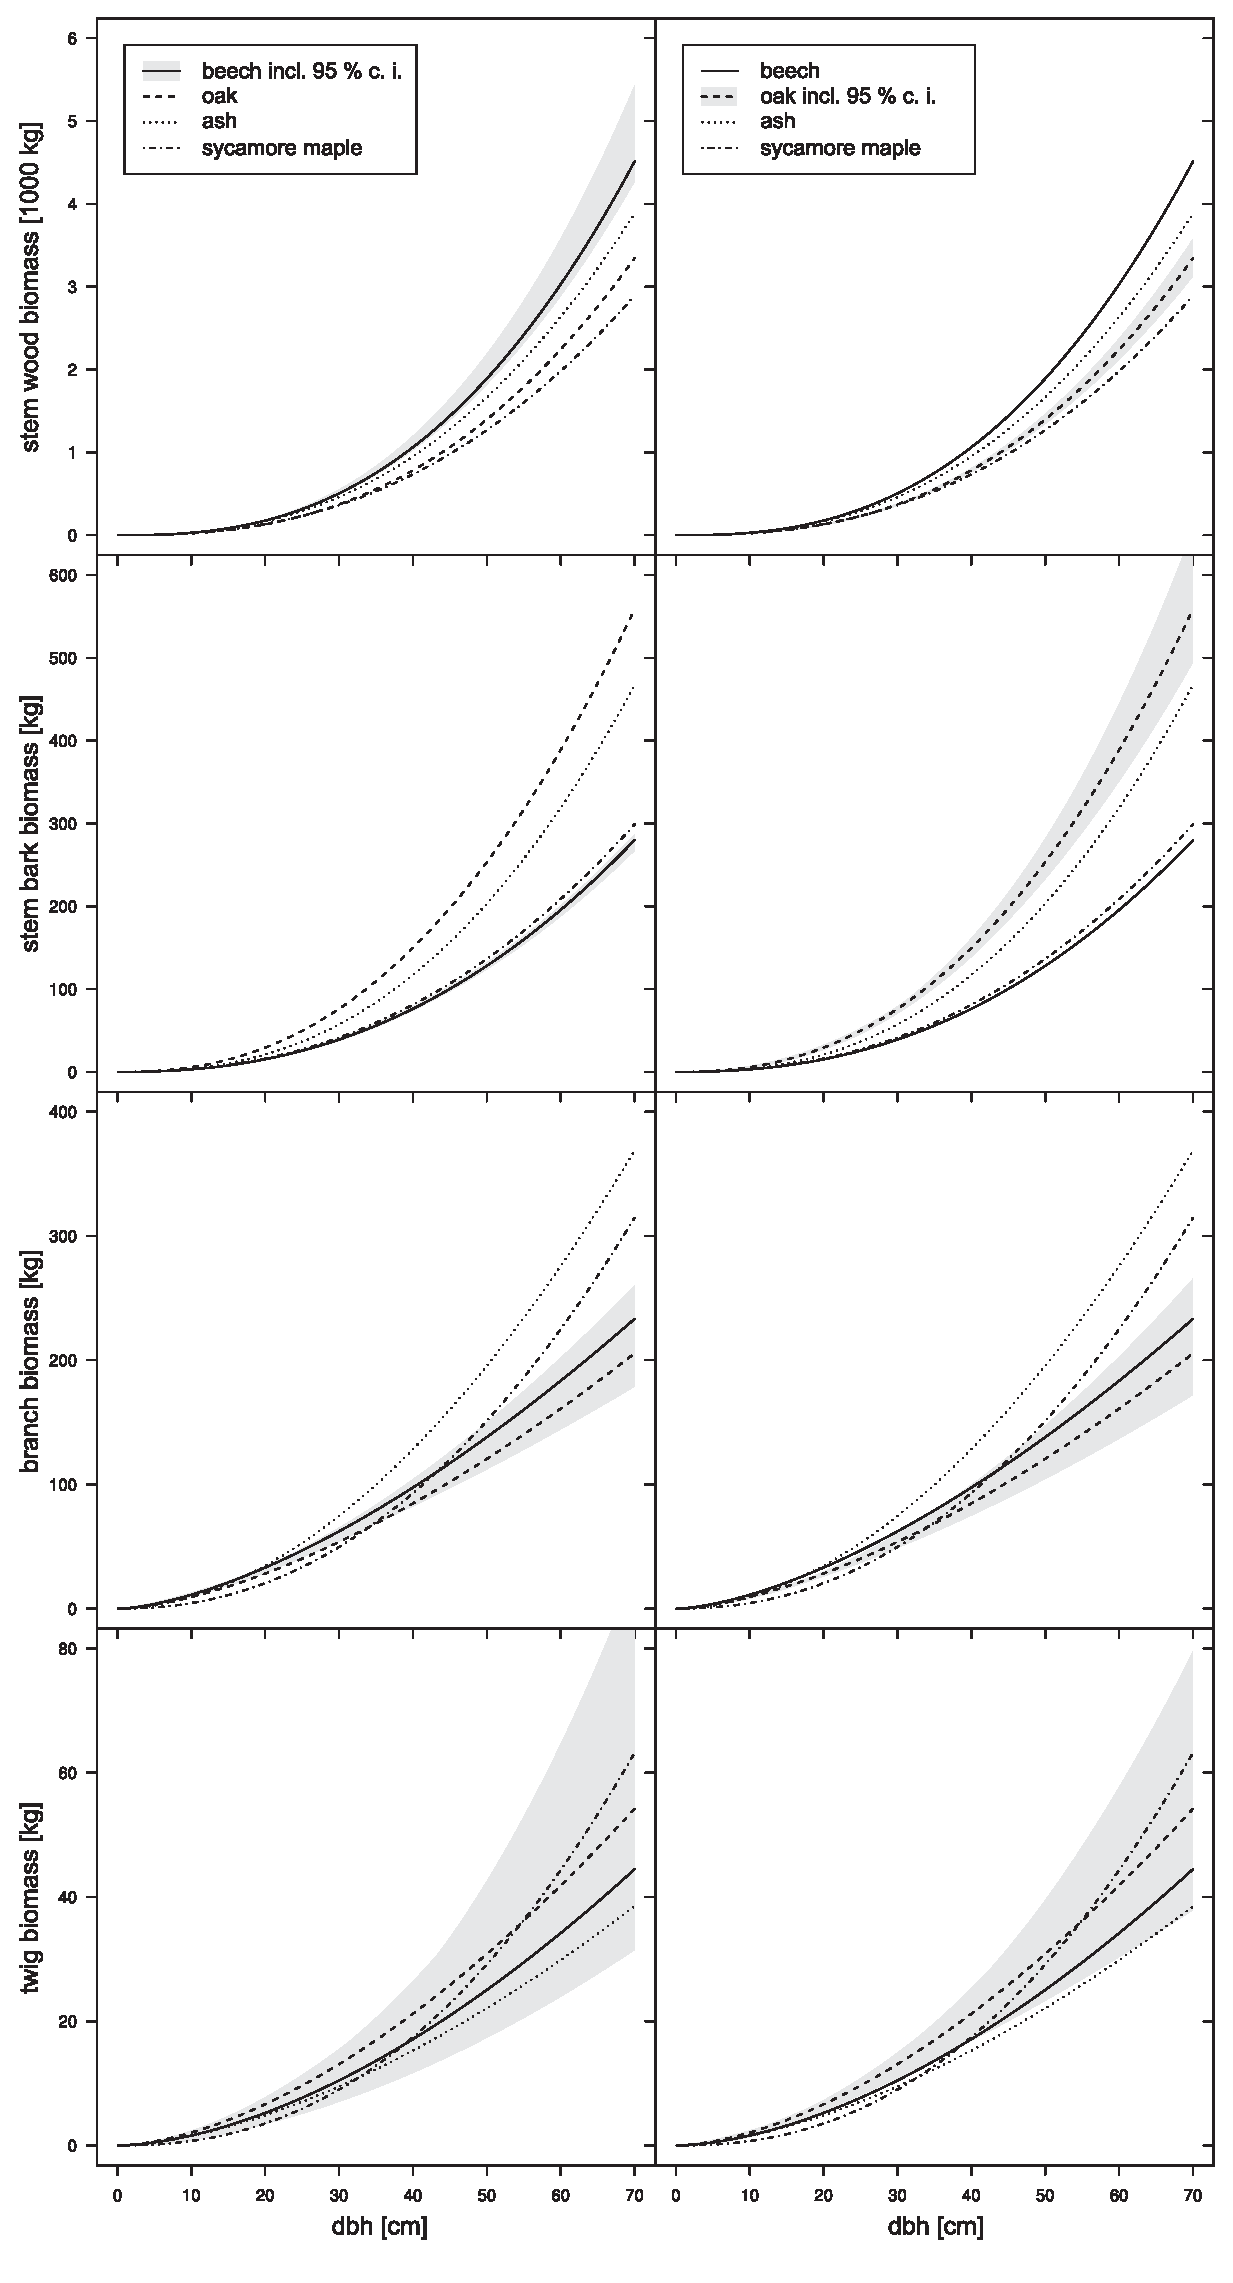
\includegraphics[width=0.7\textwidth]{Grafiken/bm/Fig_2_Regression_curves.eps}
	\caption{Regression of the biomass functions for European beech, oak, ash and sycamore over dbh. The left column includes a 95 \% confidence interval for the European beech regression function. The right column shows the same regression functions including a 95 \% confidence interval for the oak function.}
	\label{fig:bm:fig2}
\end{figure}

A comparison of the biomass models should show whether separate biomass functions for sycamore and ash are necessary. For this purpose confidence intervals were generated for the European beech and oak functions (Figure \ref{fig:bm:fig2}). We chose the 2-parametric functions with dbh as only descriptive variable for the model comparison. For stem wood there was no overlap across the whole spectrum of dbh. The curves of the stem wood functions of the 4 tree species ran more or less equidistant from one-another, with the European beech stem wood function lying above those of all other species. The lower confidence limit for the European beech stem wood function lay very near to the expected value. The European beech confidence interval had therefore no overlap with the other biomass functions. Although the oak stem wood function ran between the sycamore and ash functions, there was also no overlap with the other stem wood functions because the confidence intervals were comparatively narrow.

For the bark models there were also no areas of overlap between the graphs. The bark biomass functions could be separated into 2 groups. The graph of the sycamore bark biomass function ran very near to that of European beech. Due to the relatively large data pool and the small data variance, the confidence intervals for the European beech models were very narrow so, despite the proximity on the graph, there was no overlap with the sycamore function. The bark biomass functions for ash and oak lay almost twice as high on the graph as those of European beech and sycamore. The confidence interval of the oak function was much wider than the European beech confidence interval. The distance between the oak and ash functions is, however, so large that there was no overlap between the two.

The confidence intervals of the branch functions were altogether much wider than those of the stem wood and bark functions. The confidence interval of the European beech branch model enclosed the oak function and vice-versa. The sycamore function for branch biomass overlapped with the European beech confidence interval in the dbh range between 35 - 50 cm and with the oak function confidence interval in the range 30 - 45 cm. The graphs of the sycamore and ash branch biomass functions were, however, much steeper. Consequently there is a clear difference between the sycamore and ash branch models to the European beech and oak models.

The graphs of the 4 twig biomass models were indistinguishable over most of the value range. The confidence intervals of these functions were very asymmetric and even wider than the branch function confidence intervals. The confidence interval of the European beech function was the widest and enclosed all the other functions across the whole diameter range. The confidence interval of the oak function was slightly narrower and enclosed the European beech and sycamore functions from a dbh of ca. 40 cm and higher. The function graph of the sycamore function ran within the confidence intervals of both European beech and oak over much of the dbh value range. It was, however, much steeper than all other models. The graph of the ash function lies close under that of the European beech function. Consequently, the twig functions are mostly indistinguishable by means of the confidence interval analysis although their curvature is partially different.

The proportion of stem wood in the tree biomass increased disproportionately high with increasing dbh. For the oak functions the stem wood percentage increased sharply at first, from 56 \% by dbh 10 cm to 68 \% by dbh 20 cm. By dbh 60 cm the stem wood share of the biomass was 79 \% but did not increase much further after that. On average the stem wood share was 72 \%. The proportion of the bark biomass was more or less constant at ca. 14 \%. The share of branch as well as twig biomasses decreased with increasing dbh. The share reduced from 26 \% to 5 \% for branch and 4 \% to 1 \% for the twig biomass in the observed diameter range. The relationships between the tree fractions of the other tree species were comparable. The stem wood percentage for European beech increased from 78 \% to 89 \% in the diameter range 20 cm to 60 cm, that of sycamore from 77 \% to 81 \% and ash from 73 \% to 81 \%. For each tree species the stem wood share increases digressively and nears an asymptote. Above a dbh of ca. 60 cm the stem wood share in the tree species studied did not change much. The share of bark in the total biomass for European beech (6 \%) sycamore (9 \%), and ash (10 \%) remained relatively constant. The share of biomasses in branches and twigs thus also decreased with increasing dbh for those 3 tree species.

\begin{figure}
	\center
	\includegraphics[width=0.7\textwidth]{Grafiken/bm/Fig_3_Fraction_Biomass.eps}
	\caption{Biomass of the tree fractions in absolute scale (left) and relative to the total aboveground biomass (right) over dbh for oak.}
	\label{fig:bm:fig3}
\end{figure}

%%----------------------%%
%% Sensitivity analysis %%
%%----------------------%%
\subsection{Sensitivity analysis}
\label{subsec:bm:results:sensitivity}

In order to assess the magnitude of the effect that different biomass functions can have on results at the stand level, real and simulated test stands were used (Tables \ref{tab:bm:tab2} and \ref{tab:bm:tab4}). The sum of the total aboveground biomasses for all trees in these stands was firstly calculated with the tree species specific biomass functions. Then, secondly, the sum of the total aboveground biomasses was again calculated using only the oak biomass functions for estimating biomasses of sycamore and ash trees. The full tree biomass at the stand level for the first test stand (proportion European beech: 75 \%) was calculated to be ca. 200 t ha$^{-1}$ when using tree specific biomass functions. Using oak biomass functions for sycamore and ash led to a 4 \% overestimation of the stand biomass (ca. 7 t ha-1). The difference between the two calculation methods increased steadily with a decreasing proportion of European beech, reaching a maximum overestimation of 11 \% (21 t ha$^{-1}$) for a stand with an equal tree species mixture. If the proportion of European beech was held constant, then the difference of the total aboveground biomass on stand level increased with a decreasing ash percentage in the stand. In every case the estimated total biomass at the stand level was lower when separate, species specific, biomass functions were used.

\begin{table}[]
	\centering
	\caption{Sum of total aboveground biomass on stand level for stands with differing share of species. The biomass is calculated with distinct tree species specific biomass functions and also with oak biomass functions for ash and sycamore.}
	\label{tab:bm:tab4}
	\begin{tabular}{cccccc}
		\cline{1-3} \cline{5-6}
		\multicolumn{3}{c}{share {[}\%{]}}                                        &  & \multicolumn{2}{c}{total aboveground biomass {[}t ha$^{-1}${]}}                                                                                  \\ \cline{1-3} \cline{5-6} 
		\begin{tabular}[c]{@{}c@{}}European\\ beech\end{tabular} & ash & sycamore &  & \begin{tabular}[c]{@{}c@{}}tree specific\\ functions\end{tabular} & \begin{tabular}[c]{@{}c@{}}oak functions for\\ ash and sycamore\end{tabular} \\ \cline{1-3} \cline{5-6} 
		75                                                       & 12  & 12       &  & 199.4                                                             & 206.8                                                                        \\
		68                                                       & 25  & 7$^*$    &  & 201.6                                                             & 208.6                                                                        \\
		68                                                       & 16  & 16       &  & 199.0                                                             & 210.1                                                                        \\
		68                                                       & 7   & 25       &  & 194.5                                                             & 206.9                                                                        \\
		50                                                       & 25  & 25       &  & 197.3                                                             & 213.1                                                                        \\
		33                                                       & 33  & 33       &  & 188.1                                                             & 208.8                                                                        \\ \cline{1-3} \cline{5-6}
		\multicolumn{6}{l}{*Original test site (Table \ref{tab:bm:tab2})}
	\end{tabular}
\end{table}

%%-------------------%%
%% Nutrient contents %%
%%-------------------%%
\subsection{Nutrient contents}
\label{subsec:bm:results:nutrients}

In our analysis, the nutrient contents differed particularly between the tree species. In order to examine significant differences, we performed a parametric one-way analysis of variance for each nutrient and fraction combination with 5 \% significance level. The mean nutrients contents are listed in Table \ref{tab:bm:tab5}. All of the nutrient content data in the fraction and species groups were approximately normally distributed. For this, simple arithmetic group means are sufficient for data description and model building. This mean nutrients contents allows the tree and fraction specific calculation of the nutrients by multiplying its biomass with the respective element content from Table \ref{tab:bm:tab5}.

% Please add the following required packages to your document preamble:
% \usepackage{multirow}
\begin{table}[]
	\centering
	\caption{Group mean and standard deviation of nutrient content [g kg$^{-1}$] for the tree species European beech, oak, ash and sycamore. N: Observed number of trees.}
	\label{tab:bm:tab5}
	\begin{tabular}{ccccccccc}
		\hline
		spec.                                                                        & frac.                                                                & Ca           & Mg           & K            & C             & N            & P            & S            \\ \hline
		\multirow{8}{*}{\begin{tabular}[c]{@{}c@{}}oak\\ N=8\end{tabular}}           & \multirow{2}{*}{\begin{tabular}[c]{@{}c@{}}stem\\ wood\end{tabular}} & 0.729        & 0.100        & 1.131        & 495.898       & 1.895        & 0.087        & 0.126        \\
		&                                                                      & ($\pm$0.592) & ($\pm$0.090) & ($\pm$0.362) & ($\pm$6.515)  & ($\pm$0.736) & ($\pm$0.060) & ($\pm$0.038) \\
		& \multirow{2}{*}{bark}                                                & 26.350       & 0.768        & 2.363        & 484.346       & 6.518        & 0.276        & 0.622        \\
		&                                                                      & ($\pm$6.787) & ($\pm$0.401) & ($\pm$0.789) & ($\pm$45.123) & ($\pm$1.602) & ($\pm$0.090) & ($\pm$0.237) \\
		& \multirow{2}{*}{branch}                                              & 6.347        & 0.522        & 1.954        & 492.667       & 5.165        & 0.323        & 0.333        \\
		&                                                                      & ($\pm$2.882) & ($\pm$0.169) & ($\pm$0.223) & ($\pm$5.918)  & ($\pm$1.362) & ($\pm$0.091) & ($\pm$0.115) \\
		& \multirow{2}{*}{twig}                                                & 7.368        & 0.813        & 3.050        & 504.286       & 10.531       & 0.769        & 0.621        \\
		&                                                                      & ($\pm$2.727) & ($\pm$0.379) & ($\pm$0.395) & ($\pm$7.683)  & ($\pm$1.285) & ($\pm$0.089) & ($\pm$0.103) \\ \hline
		\multirow{8}{*}{\begin{tabular}[c]{@{}c@{}}beech\\ N=18\end{tabular}}        & \multirow{2}{*}{\begin{tabular}[c]{@{}c@{}}stem\\ wood\end{tabular}} & 0.968        & 0.302        & 1.135        & 493.686       & 1.492        & 0.100        & 0.091        \\
		&                                                                      & ($\pm$0.156) & ($\pm$0.132) & ($\pm$0.248) & ($\pm$6.100)  & ($\pm$0.520) & ($\pm$0.056) & ($\pm$0.016) \\
		& \multirow{2}{*}{bark}                                                & 22.738       & 0.517        & 2.351        & 487.684       & 6.855        & 0.351        & 0.331        \\
		&                                                                      & ($\pm$7.651) & ($\pm$0.191) & ($\pm$0.413) & ($\pm$22.248) & ($\pm$1.370) & ($\pm$0.093) & ($\pm$0.053) \\
		& \multirow{2}{*}{branch}                                              & 3.150        & 0.371        & 1.559        & 493.113       & 2.805        & 0.243        & 0.148        \\
		&                                                                      & ($\pm$1.536) & ($\pm$0.140) & ($\pm$0.309) & ($\pm$7.705)  & ($\pm$0.520) & ($\pm$0.124) & ($\pm$0.019) \\
		& \multirow{2}{*}{twig}                                                & 6.883        & 0.524        & 2.989        & 508.817       & 8.427        & 0.791        & 0.479        \\
		&                                                                      & ($\pm$2.839) & ($\pm$0.266) & ($\pm$0.569) & ($\pm$8.408)  & ($\pm$1.039) & ($\pm$0.297) & ($\pm$0.054) \\ \hline
		\multirow{8}{*}{\begin{tabular}[c]{@{}c@{}}ash\\ N=37\end{tabular}}          & \multirow{2}{*}{\begin{tabular}[c]{@{}c@{}}stem\\ wood\end{tabular}} & 0.823        & 0.193        & 1.654        & 493.495       & 1.448        & 0.092        & 0.113        \\
		&                                                                      & ($\pm$0.148) & ($\pm$0.08)  & ($\pm$0.313) & ($\pm$5.497)  & ($\pm$0.342) & ($\pm$0.036) & ($\pm$0.044) \\
		& \multirow{2}{*}{bark}                                                & 25.505       & 0.657        & 5.067        & 477.649       & 5.312        & 0.291        & 0.469        \\
		&                                                                      & ($\pm$7.428) & ($\pm$0.165) & ($\pm$1.397) & ($\pm$10.354) & ($\pm$0.644) & ($\pm$0.065) & ($\pm$0.071) \\
		& \multirow{2}{*}{branch}                                              & 4.815        & 0.319        & 2.524        & 492.675       & 2.988        & 0.228        & 0.245        \\
		&                                                                      & ($\pm$2.138) & ($\pm$0.079) & ($\pm$0.521) & ($\pm$5.58)   & ($\pm$0.647) & ($\pm$0.075) & ($\pm$0.061) \\
		& \multirow{2}{*}{twig}                                                & 8.691        & 0.83         & 6.344        & 491.191       & 8.359        & 0.769        & 0.73         \\
		&                                                                      & ($\pm$1.689) & ($\pm$0.202) & ($\pm$0.775) & ($\pm$5.982)  & ($\pm$1.175) & ($\pm$0.202) & ($\pm$0.091) \\ \hline
		\multirow{8}{*}{\begin{tabular}[c]{@{}c@{}}syca-\\ more\\ N=25\end{tabular}} & \multirow{2}{*}{\begin{tabular}[c]{@{}c@{}}stem\\ wood\end{tabular}} & 1.068        & 0.322        & 1.403        & 497.572       & 1.467        & 0.111        & 0.118        \\
		&                                                                      & ($\pm$0.26)  & ($\pm$0.129) & ($\pm$0.268) & ($\pm$3.725)  & ($\pm$0.186) & ($\pm$0.021) & ($\pm$0.021) \\
		& \multirow{2}{*}{bark}                                                & 25.184       & 0.861        & 3.784        & 474.982       & 7.737        & 0.57         & 0.772        \\
		&                                                                      & ($\pm$7.479) & ($\pm$0.21)  & ($\pm$1.027) & ($\pm$10.544) & ($\pm$1.502) & ($\pm$0.144) & ($\pm$0.134) \\
		& \multirow{2}{*}{branch}                                              & 4.089        & 0.491        & 2.394        & 493.285       & 3.403        & 0.318        & 0.283        \\
		&                                                                      & ($\pm$1.673) & ($\pm$0.122) & ($\pm$0.335) & ($\pm$4.084)  & ($\pm$0.654) & ($\pm$0.068) & ($\pm$0.059) \\
		& \multirow{2}{*}{twig}                                                & 9.668        & 0.815        & 3.889        & 495.799       & 9.948        & 0.898        & 0.709        \\
		&                                                                      & ($\pm$3.011) & ($\pm$0.227) & ($\pm$0.79)  & ($\pm$6.299)  & ($\pm$2.602) & ($\pm$0.268) & ($\pm$0.137) \\ \hline
	\end{tabular}
\end{table}

With ca. 500 g kg$^{-1}$ (dry biomass) in stem wood, as well as in bark, carbon has the greatest share of any element content in the entire dry weight. The average carbon content lies between 475 g kg$^{-1}$ and 509 g kg$^{-1}$, with slight differences between the tree species and fractions. In the stem wood sycamore differs significantly from beech while the carbon contents of other combinations do not differ significantly. In the bark fraction, ash and sycamore differ significantly from oak and beech. For sycamore and ash, the carbon content in the stem bark is a little lower than in the stem wood. The average nutrient contents, with the exception of a few calcium contents in the branches of sycamore and ash, were < 25 g kg-1. With few exceptions, the content of the various nutrients in wood can be ranked as follows: N > K > Ca > Mg > P = S. Ash has the largest potassium content (1.65 g kg$^{-1}$) of all 4 tree species. The potassium content in ash is throughout significantly higher than in all other examined species. In terms of the magnesium content, the trees can be separated into two groups. The mean content is significantly higher for sycamore and European beech than for oak and ash. Generally, the nutrient contents in bark are between 3 (N, P and K) and 25 (Ca) times higher than in wood. The concentrations of nitrogen, phosphor and sulfur in sycamore bark are always significantly higher than those of European beech and than those in the bark of oak and ash. The bark of ash has significantly lower nitrogen concentrations than the other species but higher potassium content.

\begin{figure}
	\center
	\includegraphics[width=1\textwidth]{Grafiken/bm/Fig_4_nutrient_eff_1.eps}
	\caption{Nitrogen (N), calcium (Ca) and potassium (K) nutrient response efficiency for European beech, ash and sycamore when harvesting stem wood (including bark) only in comparison to a full tree usage.}
	\label{fig:bm:fig4}
\end{figure}

The nutrient response efficiency per tree species was calculated for the European beech - broad leaf mixed test stand (Table \ref{tab:bm:tab2}). In Figures \ref{fig:bm:fig4} and \ref{fig:bm:fig5}, the results for the respective tree species and tree fractions are shown. The nutrient response efficiencies for stem wood usage were calculated by dividing the carbon concentrations in the fractions stem wood and bark by the respective nutrient concentrations. Analogously, the nutrient response efficiencies for full tree usage were achieved by dividing the carbon concentrations of all 4 fractions by the particular nutrient concentrations. With reference to potassium, calcium and sulfur, European beech had the most efficient biomass production and, therefore, the most efficient carbon sequestration rate. Ash had the lowest nutrient efficiency for calcium and potassium, while phosphorus was used just as efficiently by ash as by European beech. With reference to magnesium, ash was the most efficient species and sycamore the least, while there was no real difference in efficiency between the 4 tree species with regard to nitrogen.

\begin{figure}
	\center
	\includegraphics[width=1\textwidth]{Grafiken/bm/Fig_5_nutrient_eff_2.eps}
	\caption{Phosphor (P), sulphur (S) and magnesium (Mg) nutrient response efficiency for European beech, ash and sycamore when harvesting stem wood (including bark) only in comparison to a full tree usage.}
	\label{fig:bm:fig5}
\end{figure}

Because the branches and twigs are only used if the full tree is harvested, it seemed worth comparing the nutrient response efficiency of the stem wood biomass with that of the total aboveground biomass. The comparison revealed that the nutrient response efficiency of the total above ground biomass was always between 5 \% and 10 \% lower than that of the stem wood biomass. This trend can be observed for all examined tree species.



%%%%%%%%%%%%%%%%
%% Discussion %%
%%%%%%%%%%%%%%%%
\section{Discussion}
\label{sec:bm:discussion}

%%-------------------%%
%% Biomass functions %%
%%-------------------%%
\subsection{Biomass functions}
\label{subsec:bm:discussion:bm_functions}
In comparison to other existing function types, such as those of \citet{ledermann_2006}, \citet{eckmullner_2006} and \citet{marklund_1988}, the biomass model from \citet{hochbichler_2006} (Equation \ref{eq:bm:eq1}) proved, after extensive AIC and residual analyses, to be the most suitable. The model was fitted directly nonlinear without data transformation. There was thus no need for a subsequent bias correction \citep{baskerville_1972, smith_1993}. Due to the sufficiently large data pool the entire bandwidth of forestry relevant tree dimensions is covered by our biomass functions. A mixed effect regression model with distinct error structure for regional clusters did not improve our models. We therefore did not consider any mixed effect.

In large parts, the quality of the models depended on the tree fraction being examined (Table \ref{tab:bm:tab3}). The branch and twig models showed a higher variation in comparison with the stem wood and bark models. The accuracy of estimation of all stem wood and bark models could, though, be improved by including tree height in the models. If the appropriate data is available, then these more complex models are preferable. This was confirmed performing analysis of AIC, $v(\hat{y})$ and $r_{LR}^{2}$ (Table \ref{tab:bm:tab3}).

The nonlinear pseudo-r-squared can be interpreted as the proportion of explained variation. There are, nevertheless, unlike the linear r-squared, several possibilities of calculating it \citep{magee_1990}. The likelihood-ratio pseudo-r-squared $r_{LR}^2$ are thus often not directly comparable to the r-squared of other studies. It, however, becomes apparent that our r-squared are roughly in line with all r-squared found in literature (see e.g. \citet{zianis_2005} for a broad overview). In most other studies the r-squared of the stem and bark models amount at least to 0.9. The same appears for the branch and twig models. With values ranging from 0.6 to 0.8, the r-squared are much smaller.

Other studies \citep{ledermann_2006, pretzsch_2014} have shown that other variables could also improve model accuracy. Including tree height, tree height at crown base, crown width, tree age and a dummy code for forked tree lowered model standard error for the European beech biomass model by ca. 6 \% and the oak model by ca. 13 \%, when compared to the dbh-only model in a study of \citet{ledermann_2006}. These results couldn�t be replicated in this study. Only tree age led, in a few cases, to a significant, though very small, model improvement. The age of individual trees is, however, seldom surveyed in the practice, so age was not further considered in creating the models. \citet{hochbichler_2006}, who developed branch biomass functions for oak and European beech, observed a slight model improvement of the beech model when using the crown ratio as additional independent variable. We were not able to reproduce this result with our data. The crown ratio was not significant in any model. The same was found for the tree height to tree diameter ratio. As we collected our data in pure stands under standard regimes, the influence of the mixture and concurrence on the allometry, as it was e.g. observed by \citet{pretzsch_2012}, could not be analysed.

Using a simple nonlinear regression for the tree fractions meant that any within-species correlation (collinearity) between fractions was not taken into account. This is of course a simplification. Since collinearity would have led to a huge difference between the distinct coefficients of variation and the combined coefficients of variation and we observed only minor differences (Table \ref{tab:bm:tab3}), it becomes clear that collinearity in the model had no considerably negative effect on any model. The combined model coefficients of variation were primarily influenced by the stem wood and bark models, variation in the branch and twig models had very little influence. There was thus only high correlation between fractions with comparatively low variation. The highest impact of collinearity was found for the sycamore biomass functions. The dimension of the combined coefficient of variation, however, was still very small. It can therefore be assumed that collinearity did not limit the validity of any model. Further analyses with simultaneous regression methods, such as a Seemingly Unrelated Regression \citep{henningsen_2007} or Restricted Regression, could establish whether the model error could be further reduced by considering collinearity during the regression. At any rate, the results of the analyses undertaken here indicate a valid estimation of the model parameters. Simultaneous methods could probably reduce the model variance significantly. Other studies, for instance \citet{sanquetta_2015}, came to the same conclusion. Using tree growth data they were able to show that the parameter estimations were close to the results when using both separate and simultaneous estimations, whereas the variance, and with it the model efficiency, could be improved by using simultaneous methods.

Due to the relatively small variance in the raw data, the confidence intervals for the stem wood and stem wood bark functions were, as expected, narrower than the confidence intervals for the branch and twig models in the model comparison (Figure \ref{fig:bm:fig2}). Owing to the very wide confidence interval calculated for the European beech twig function, it is only for the twig models that the biomass functions of other species overlapped with the European beech confidence interval. Because of the relatively large scattering of the twig (see also Table \ref{tab:bm:tab3}), the sycamore and ash twig functions could be substituted by the European beech function. The curve of the sycamore function, however, differed markedly from the other function curves. It should also be noted, that the twig biomass makes up only a small proportion of the total biomass.

The functions were compared using the 2-parameter models, with dbh as the single covariate, revealing clear differences in the biomass models. Using 3-parameter models, with tree height included as an additional variable, would reveal at least the same model differences. The addition of other significant variables would narrow the confidence bands even further, due to the reduced variance (Table \ref{tab:bm:tab3}). In conclusion, the comparison of the biomass functions obviously underlines the need for separate sycamore and ash functions. The biomass functions of these species differ clearly from the beech and oak functions. The estimation of single tree biomass for sycamore and ash using biomass functions for other tree species, which up to now has been the norm, certainly leads to biomass estimation errors.

The proportion of stem wood increases with increasing dbh (Figure \ref{fig:bm:fig3}). This increase in the stem wood proportion with increasing dbh could also be documented for European beech in the diameter range 6 - 16 cm by \citet{grote_2003}. They observed an increase of the average stem wood proportion from 30 \% to 80 \%, which is very close to the results from this study (Figure \ref{fig:bm:fig3}) for that diameter range. The data used by \citet{grote_2003} were sampled in a mixed oak - pine stand, which indicates that the relationship of stem wood biomass is similar in these stands, at least in the diameter range 6 - 16 cm. \citet{konopka_2015} also recorded an increase in the stem volume of young European beech up to 4 cm dbh, while \citet{cienciala_2005} and \citet{pretzsch_2014} observed a stem wood share between 70 \% and 90 \%, with a mean of 82 \%. This mean share is also similar to the data from this study (Figure \ref{fig:bm:fig3}), though neither of these 2 studies found a significant diameter trend. \citet{genet_2011} observed a shifting of the stem wood share from 60 \% to 75 \% in trees between 13 and 81 years old, which is also consistent with the results of this study. The stem wood bark percentage from our study of 6 \% is consistent with all values found in the literature \citep{altherr_1978, grote_2003, pretzsch_2014}. The fraction proportions of oak also showed a diameter trend. The stem wood proportion has a rising tendency, but lies clearly under the stem wood proportion of European beech. The stem wood percentage of 68 \% to 80 \% in the 20 cm to 60 cm diameter range corresponds well with the data from \citet{pretzsch_2014}, who observed a mean percentage of 75 \%. \citet{grote_2003} observed an increase of the stem wood percentage from 61 \% to 71 \% in the dbh range 10 cm to 30 cm, which is again very close to the results presented here. The bark proportion is also consistent with the literature values \citep{altherr_1978, pretzsch_2014}, whereby \citet{altherr_1978} found a site dependency. Comparison of the fractions relations of ash and sycamore with literature functions were, due to differing fractionations, not possible. Comparison of the total aboveground biomass reinforces the validity as well as the importance of our models. It could be seen that our functions were slightly different to all other models found in the literature \citep{albert_2014, alberti_2005, bunce_1968}. As an example, our ash as well as our sycamore functions lay in between the functions of \citet{albert_2014}, who parameterized distinct functions with trees from a rich and a poor coppice stand. Although there are differences in the parameter estimations between the new parameterized functions in our study to former studies, the general proportions seem to be consistent with other biomass functions for all 4 tree species. This was expected as biomass functions are known to have regional differences \citep{cerny_1990, thurnher_2013}. Publishing specific biomass function for the northern and central part of Germany seems thus to be worthwhile for all 4 species.

%%----------------------%%
%% Sensitivity analysis %%
%%----------------------%%
\subsection{Sensitivity analysis}
\label{subsec:bm:discussion:sensitivity}
Biomass of ash and sycamore must recently be estimated by biomass function of other species. To assess the magnitude of the effect these false estimations can have on biomass estimations in the praxis, test stands were generated (Tables \ref{tab:bm:tab2} and \ref{tab:bm:tab4}). The oak biomass function was preferred to the European beech function for these analyses, because the curve of the oak function was a better fit with the sycamore and ash function curves (Figure \ref{fig:bm:fig2}). The results reinforce the need for separate biomass functions. As observed before, especially the sycamore functions were different to the oak biomass functions. In particular for sycamore the estimate was substantially improved with a separate species specific biomass function. In stands with a high proportion of sycamore, estimating biomass using oak functions led to massive overestimation of the biomass and the sequestered carbon (Table \ref{tab:bm:tab4}). The same effect would also be evident in the products of forestry use and the downstream transport chain. The actual biomass potential would be considerably lower than the predicted potential. With respect to the fact that accurate biomass predictions are mandatory for a reliable biomass potential estimation, this underestimation, as it was obligatory until now, seems not to be acceptable.

%%-------------------%%
%% Nutrient contents %%
%%-------------------%%
\subsection{Nutrient contents}
\label{subsec:bm:discussion:nutrients}
Varying nutrient contents, not only between tree species but also between tree fractions, has been demonstrated in many studies for European beech and oak before (e.g. \citet{augusto_2000, muller-using_2004, pretzsch_2014}). In this study these differences in nutrient content were also shown for sycamore and ash (Table \ref{tab:bm:tab5}). In comparison to European beech and oak, ash and sycamore species have significantly higher calcium and potassium contents and significantly less carbon contents. Export of sycamore and ash biomass will thus be underestimated, if European beech or oak contents are used for their estimation. In other studies (e.g. \citet{joosten_2003}), it was shown that nutrient contents also significantly depended on the site quality. As sycamore and ash only grow on sites of relatively high quality, our sample for the chemical analysis comprised rich stands only. The stand quality thus had of course no significant explanatory content in our study. The nutrient contents are generally higher in the bark than in the wood and this applies to all 4 studied tree species. Because the proportion of bark within a tree decreases with increasing branch diameter, small diameter wood fractions (branches and twigs) have higher nutrient concentrations.

This is reflected in lower nutrient response efficiencies for these fractions \citet{vitousek_1982, rumpf_2011, meiwes_2012}. A greater amount of nutrients has been used in building biomass in these smaller fractions than are needed to build the same biomass in stem wood. Except for nitrogen, the calculated nutrient response efficiencies were substantially different for the observed tree species. This again reinforces the need for distinct biomass and nutrient content models. It must, however, be considered that our definition of the nutrient efficiency is slightly different to the original definition by \citet{vitousek_1982}. He stated that in long-living perennial plants the nutrient efficiency calculates as the inverse of the nutrient concentration in the wood increment, the litterfall and the root turnover. As none of those variables was measured in our study and because the litterfall as well as the root turnover remain in the stand, their efficiency is not relevant for the calculation of the biomass potential. We thus only focused on the nutrient content of the aboveground biomass. The use of small dimensioned wood leads to a disproportionately high nutrient loss and has a greater negative effect on the nutrient supply of the site than stem wood harvest alone \citep{block_2012, meiwes_2012, pretzsch_2014}. On the other hand, in times of modern processing methods, in precisely those recently often unused wood fractions there is a huge potential for the bio-based industry.

%%%%%%%%%%%%%%%%%
%% Conclusions %%
%%%%%%%%%%%%%%%%%
\section{Conclusions}
\label{sec:bm:conclusions}
When coupled with individual site information, the results of this study help determining the optimal biomass potential of mixed stands with European beech, oak, sycamore and ash. In forest stands with homogeneous tree species and age distributions the biomass and nutrient quantities could certainly be estimated with sufficient accuracy using stand parameters such as mean basal tree area \citep{pretzsch_2014}. As is made clear by the example in Table \ref{tab:bm:tab4}, this is not possible in mixed broadleaf stands. The use of the oak biomass function for all tree species would lead to overestimating both biomass and nutrient quantities. Because the share of multiple layer, species-rich stands in forests is increasing \citep{ti_2014}, and will probably continue to increase \citep{bmel_2014}, the need for species specific biomass functions becomes ever more urgent. For estimating the optimal site specific harvest quantities, biomass functions, and knowledge of tree fraction nutrient content, for the tree species sycamore and ash are a useful addition to already existing functions, and could help to enable the full biomass potential of the forest to be exploited in the future. They improve the planning security of forestry activities and of all further processes in the biomass supply chain and help to analyse the trade-off between usage intensity and site sustainability. All further analyses that require reliable biomass estimations, for example supply analysis for operative and strategic planning or carbon inventories, will also profit from the biomass functions introduced here. The introduced models can help gathering the huge biomass potential from long-term broadleaf stands that was unused till now \citep{ti_2014}.

%%%%%%%%%%%%%%%%%%%%%%
%% Acknowledgements %%
%%%%%%%%%%%%%%%%%%%%%%
\section*{Acknowledgements}
\label{sec:bm:acknowledgements}
The authors are grateful to the Project Management J�lich of the Federal Ministry of Education and Research for funding this research through the projects \textit{BEST} (003L033F) and Cluster \textit{Bio-Economy} (031A294) as well as to the Agency for Renewable Resources of the Federal Ministry for Consumer Protection, Food and Agriculture for funding the project \textit{M�glichkeiten und Grenzen der Vollbaumnutzung} (22015407). We would like to thank the anonymous reviewers for their helpful and constructive revision of the manuscript.

	%\cleardoublepage
	\chapter{Modelling the economically viable wood in the crown of European beech trees}
\label{chap:beech_crowns}
{\large Kai Husmann$^1$ - Bernhard M�hring$^1$}\\

\vspace{3cm}
\noindent
$^1$Department of Forest Economics and Forest Management,\\ University of G�ttingen, B�sgenweg 3, 37077 G�ttingen, Germany \\

\vspace{\fill}
\noindent
Published in:\\
\textit{Forest Policy and Economics} 78 (2017): 67-77 \\(DOI: 10.1016/j.forpol.2017.01.009)

\newpage
\begin{itemize}
	\item Bernhard M�hring supported analysis of the results, writing of the manuscript and the review process.
\end{itemize}

\cleardoublepage
%%%%%%%%%%%%%%
%% Abstract %%
%%%%%%%%%%%%%%
\section*{Abstract}
\label{chap:beech_crowns:Abstract}
Long-term forest development programs in Germany aim on an increase of close-to-nature broadleaf forest stands. This means that the economic importance of European beech is expected to increase. The economic potential of a tree basically consists of the stem as well as the economically viable wood volume in the crown. Due to the high morphological variability of European beech crowns, taper models are often not satisfactory for predicting the economically viable wood volume arising from crowns. Prediction models with a higher precision are recently still lacking. Aim of this study is thus the development of prediction model for the economically viable crown wood volume of European beech trees.

We determined the distribution of the wood volume in the crown over the branch diameters using the multistage \textit{randomized branch sampling} method (RBS). The tree-specific wood volume distribution on the branch diameters were used to cluster all sampled trees into 3 groups. Additionally, we developed a method able to distinguish between economically viable and unviable crown branches. Basing on the RBS measurements as well as revenues and processing costs, we modeled the economically viable wood volume from the crown for each tree. To calculate the wood volume under bark, we parameterized a bark thickness function from disk samples of the trees.

We showed that the European beech crowns could be clustered into 3 groups differing in their wood volume distribution. The economically viable wood volume in the crown significantly depended on this grouping parameter as well as diameter at breast height (DBH). By contrast, the total amount of wood in the crown only depended on DBH. The differing viable wood volumes in the crowns were thus explained by different wood distributions and not by differing total crown wood volume. To make the results applicable in practice forestry, the modeling results were used to develop a regression formula able to predict the economically viable wood volume in the crown depending on the DBH and the crown type. As the crown type can also be predicted via measurable tree covariates, the regression model of the viable wood volume in the crown can be used as a support tool for the management of European beech stands. Sensitivity analysis quantifies how harvest revenues and costs translate into different viable tree volume.

\subsection*{Keywords}
Economically optimal wood cut, Crown morphology, European beech, viable crown wood, wood allocation, forest management

\subsection*{Highlights}
\begin{itemize}
\item Morphological measurements of 163 European beech tree crowns via \textit{RBS} method.
\item Distinguishing the economically viable from the whole crown wood.
\item Categorization of European beech crowns into morphological types.
\item Development of a viable crown timber prediction model for forest management.
\end{itemize}

%%%%%%%%%%%%%%%%%%
%% Introduction %%
%%%%%%%%%%%%%%%%%%
\section{Introduction}
\label{sec:beech_crowns:Introduction}
Although European beech (\textit{Fagus sylvatica L.}) forests have been identified as the dominant forest communities in the potential natural vegetation of Germany \citep{fanc_2010}, with 1,680,072 ha, they currently only account for 15 \% of Germany's forest stand cover \citep{ti_2014}. Long-term ecological forest development programs result in a general increase in deciduous tree species with a focus on European beech \citep{mfacp_2004}. The economic importance of European beech will thus further increase.

Traditionally the objective of European beech management is to maximize valuable stem wood \citep{nagel_2008}. Especially under the perspective of modern utilization methods like bio-economics \citep{hildebrandt_2014} and the increasing demand for fuel wood \citep{mantau_2012}, the economic importance of smaller branches of European beech is expected to increase. Thus a large proportion of the economic potential lies in smaller branches. Under certain conditions, further economic potential can be found in the tree stump and foliage \citep{miettinen_2014}. For a suitable management of European beech stands, it is necessary to assess the economically viable wood cut fully \citep{mohring_1997}. Therefore, as well as predicting the wood from the sympodial stem, it is also necessary to predict the economically viable wood cut in the sympodial crown. In the complex crowns of broadleaf trees, the economically viable wood can be substantially smaller than the whole wood volume. For this purpose, a model able to distinguish the economically viable wood volume from the whole wood volume in the crown is needed. For the stem volume prediction, there are many different and sophisticated tariff and other functions available. Cubic taper models exist, providing an adequate prediction of the economic potential of coniferous trees and the stems of deciduous trees \citep{kuzelka_2012}. However, those taper functions do not account for the complex sympodial form above the crown base of broadleaf tree species where the wood volume is not allocated around a throughout stem axis. They are therefore imprecise in predicting the wood volume arising above the crown base. They are usually calibrated for a minimum small-end diameter threshold of 7 cm. This small-end diameter can lack economic interpretation.

The aim of this study is to develop a parametric, practically usable prediction model of the economically viable wood volume in the crown of European beech trees. For this purpose, 163 beech trees were felled. Using the multistage \textit{Randomized Branch Sampling} (RBS) method \citep{gaffrey_1999}, a sound sample of branches was measured from each tree. The measurements were taken to examine the tree individual distribution of the wood volume in the crown on the crown branches. To develop tree individual morphological covariates, the sampled trees were clustered into groups with differing wood volume distribution. A multinomial regression model enables the prediction of this covariate via measurable tree attributes. We additionally developed a model, which predicts the viable wood volume from the measured wood volume distribution. This viable wood volume does not depend on freely selected but on economically justified small-end diameters. We developed a method to classify economically viable and unviable branches in European beech crowns via a break-even analysis. Then only the wood volumes of viable branches were estimated via RBS. The modeled economically viable wood volume thus depends on the size of the tree and the volume distribution in the crown. To calculate the wood volume under bark, we parameterized a new bark thickness function from disk samples of the trees.
To make the results applicable in forest practice, we performed a regression analysis with the modeled economically viable wood volume and further tree covariates. To ensure the applicability, we only used practically measurable tree attributes. The regression model represents a new approach for modeling the economic potential of European beech crowns and therefore a novel decision support tool for forest management operations.

%%%%%%%%%%%%%%%%%%%%%%%%%%%
%% Materials and Methods %%
%%%%%%%%%%%%%%%%%%%%%%%%%%%
\section{Materials and Methods}
\label{sec:beech_crowns:methods}
The dataset for this study comprised measurements from a destructive sample of 163 European beech trees sampled using the multistage RBS method \citep{gaffrey_1999, jessen_1955}. These data were compiled from 2 existing databases at the Northwest German Forest Research Station and the Baden-W�rttemberg Forest Research Centre.
%%-------------------------------------%%
%% Data sampling and sample processing %%
%%-------------------------------------%%
\subsection{Selection of trees}
\label{subsec:beech_crowns:methods:tree_selection}
The data were collected during 2009 and 2014. Altogether 163 trees were destructively sampled. In order to cover as many growth zones as possible, the sample plots were distributed throughout Germany (Figure \ref{fig:beech_crowns:fig1}). To ensure representation of the entire relevant diameter range, we chose up to 3 forest sites with different stand ages within these growth zones. All selected sites were high forests under standard management regimes. Depending on the area size of the plot, 2 - 4 sample trees were selected. In addition to the morphological measurements via RBS, DBH and tree height were measured (Table \ref{tab:beech_crowns:tab1}).

\begin{figure}
	\center
	\includegraphics[width=0.7\textwidth]{Grafiken/beech_crowns/Fig_1_plot_locations.eps}
	\caption{Sample site locations. Source of the background map: \citet{facg_2014}.}
	\label{fig:beech_crowns:fig1}
\end{figure}

\begin{table}[]
	\centering
	\caption{Summary statistics of the sampled trees. The sample size was 163.}
	\label{tab:beech_crowns:tab1}
	\begin{tabular}{cccc}
		\hline
		             &DBH             & height  & age \\ 
		             &[cm]            & [m]         &  [a] \\ \hline
		min          & 8.0            & 13.1        & 21      \\
		mean         & 35.4           & 25.3        & 85      \\
		median       & 34.8           & 26.0        & 80      \\
		max          & 78.3           & 38.5        & 180     \\ \hline
	\end{tabular}
\end{table}

%%--------------------%%
%% Selection of disks %%
%%--------------------%%
\subsection{Selection of disks}
\label{subsec:beech_crowns:methods:disk_selection}

To subtract bark from the wood volume, stem and branch disks for bark thickness measurement were taken from 37 trees of the NW-FVA study (Table \ref{tab:beech_crowns:tab2}). Up to 6 disks were randomly selected using the importance sampling method \citep{Gregoire_2008}. The proxy function, which is necessary for calculation of the sampling probability, was derived by the volume distribution of the branch diameters over the approximated tree height (which were both measured for volume estimation via RBS anyway). The selection probability of the disks was thus proportional to their disk diameter. Diameter and the bark thickness of the disks were measured at 4 directions of the selected disks directly after extraction.

\begin{table}[]
	\centering
	\caption{Summary statistics of disks for bark thickness measurements.}
	\label{tab:beech_crowns:tab2}
	\begin{tabular}{ccccccccccc}
		\cline{3-6} \cline{8-11}
		&  & \multicolumn{4}{c}{single bark thickness {[}mm{]}} &  & \multicolumn{4}{c}{disk diameter over bark {[}cm{]}} \\ \cline{1-1} \cline{3-6} \cline{8-11} 
		N   &  & min        & mean       & median       & max       &  & min        & mean        & median       & max        \\ \cline{1-1} \cline{3-6} \cline{8-11} 
		149 &  & 0.6        & 3.0        & 2.4          & 9.0       &  & 1.0        & 18.0        & 12.0         & 64.2       \\ \cline{1-1} \cline{3-6} \cline{8-11} 
	\end{tabular}
\end{table}

%%-----------------------%%
%% Selection of branches %%
%%-----------------------%%
\subsection{Selection of branches}
\label{subsec:beech_crowns:methods:branch_selection}
The estimation of the wood volume in the crown was based on the RBS method of multistage probability sampling. RBS is an unbiased method of probability sampling used for estimating specific tree parameters by measurable auxiliary variables \citep{jessen_1955,gaffrey_1999}. In our application, RBS enables estimation of the wood volume in the crown or in specific parts of the crown by measuring only a sample of branch segments instead of measuring all branch segments in the crown. Only relatively few measurements of branch diameters and branch segment lengths have to be taken for an accurate estimate of the whole wood volume in the crown or the wood volume of specific crown parts.

RBS is based on the knowledge of the conditional probability $q_{lj}$ of choosing the $j$-th out of n \textit{branches} at a \textit{node} $l$ in the crown instead of choosing another branch of this node. The probability $q_{lj}$ can be calculated by an auxiliary variable instead of the (complicated measurable) target variable itself \citep{gregoire_1995,Gregoire_2008,valentine_1984}. Instead of measuring the volume of all branches at a node, in our case, we only had to measure the base diameters $d_{lj}$ of the branches to calculate $q_{lj}$ and the volume of one branch. As \citet{west_1999} examined an allometric coefficient of 2.67 between branch volume and branch base diameter, the branch base diameter to the power of 2.67 is expected to provide efficient estimates. In our study, the conditional probability has been selected to be

\begin{equation}
	\label{eq:beech_crowns:eq1}
	q_{lj}(d)=d_{lj}^{2.67}/ \sum_{j=1}^{n_l} d_{lj}^{2.67}
\end{equation}

Thus once all branch base diameters $d_{li}$ at a node were recorded, one of the branches can be randomly chosen with probability $q_{lj}$. Only the \textit{segment} volume of this chosen branch has to be measured, where a \textit{segment} is defined as the part of the branch between 2 nodes \citep{Gregoire_2008}. We chose the formula for a conical frustum (Equation \ref{eq:beech_crowns:eq2}) to calculate the segment volume $v_{lj}$ via the branch base diameter $d_{lj}$, the base diameter at the following node $d_{lj+1}$ and the segment length $h_{lj}$. The volume of the following node $d_{lj+1}$ was also measured and added to the segment volume $v_{lj}$.

\begin{equation}
	\label{eq:beech_crowns:eq2}
	v_\mathit{lj}=\frac{h_{lj}\pi}{12}\left(d_{lj}^2+d_{lj}d_{{lj}+1}+d_{{lj}+1}^2\right)
\end{equation}

The crown base, which is the height where the throughout stem ends and the sympodial crown starts, represented the first node of the RBS procedure. To have a measurable criterion, we defined the crown base to be the tree height where a branch base diameter was > 1/5 of the stem diameter at that height. A whole RBS path thus consisted of a succession of randomly selected branch segments from the crown base up to one shoot bud. Along the path all branch base diameters and all segment volumes were measured. In order to get an idea of the variation, 3 random and distinct RBS paths were obtained for each of the 163 sampled trees.

%%--------------------------------------------------------%%
%% Estimation of wood volume in the stem and in the crown %%
%%--------------------------------------------------------%%
\subsection{Estimation of wood volume in the stem and in the crown}
\label{subsec:beech_crowns:methods:crown_vol_est}
The calculation method for the point estimates of the volumes as well as for the estimated variance is described in the literature \citep[e. g.][]{Gregoire_2008}. The stem form was assessed by section-wise diameter measurements at certain tree heights up to the crown base. The sum of these section volumes, also calculated by the conical frustum formula (Equation 2), gave the whole stem volume from the ground up to the crown base.

%%----------------------------------------------%%
%% Economically viable wood volume in the crown %%
%%----------------------------------------------%%
\subsection{Economically viable wood volume in the crown}
\label{subsec:beech_crowns:methods:viable}

%%++++++++++++++++++++++++++++%%
%% Crown type differentiation %%
%%++++++++++++++++++++++++++++%%
\subsubsection{Crown type differentiation}
\label{subsubsec:beech_crowns:methods:viable:crown_types}
To calculate the volume distribution according to the branch diameters in individual tree crowns, the cumulative wood volume amount $\hat{V}_i(d)$ in the crown was calculated from the crown base up to each recorded branch base diameter $(d)$ along each RBS path. This distribution was normalized by dividing the predicted cumulative crown volume below $\hat{V}_i(d)$ [m3] by the whole wood volume from the crown $\hat{V}_i(0)$ [m3] (Equation \ref{eq:beech_crowns:eq3}) and by dividing the base diameter of every branch $d_{ij}$ by the maximum diameter found $d_{max}$. $F(d)$ thus denotes the wood volume amount over branch diameter in the crown.

\begin{equation}
\label{eq:beech_crowns:eq3}
F\left(d\right)=\frac{{\widehat V}_i\left(d\right)}{\widehat V}
\end{equation}

The diameter where half of the wood volume amount was located above (below respectively) was interpreted as the median branch diameter of a tree crown. This median volume branch diameter $F(d_{0.5})$ was easily interpolated from the generated diameter distribution for every RBS path, where $d_{0.5}$ denotes the branch diameter for which $F(d_{0.5})=0.5*F(d_{max})$. The same appears for the lower $F(d_{0.25})$ and upper quantile $F(d_{0.75})$. The curve trend of $F(d)$ over branch diameter thus indicates whether most of the wood volume is located in relatively small or in larger branches. Generally, there were 3 types of volume distribution in the data (Figure \ref{fig:beech_crowns:fig2}). The first type showed a high share of volume in relatively small branch dimensions (left). The median branch diameter of these trees was close to the lower quantile. In the balanced type (center), half of the wood volume was found above a branch diameter that was approximately half the size of the largest diameter of the respective tree. In the third type (right), major part of wood volume was allocated in the larger branch diameter range. The median diameter was close to the upper quantile.

\begin{figure}
	\center
	\includegraphics[width=1\textwidth]{Grafiken/beech_crowns/Fig_2_relative_volume_amount.eps}
	\caption{Cumulative crown wood volume over relative branch diameter for 3 exemplary trees. For each tree all 3 RBS paths are displayed. The diameters where half of the timber volume is located above, respective below (the median relative branch diameter) are marked by vertical lines.}
	\label{fig:beech_crowns:fig2}
\end{figure}

As there were 3 paths per tree, the tree individual median diameter was calculated by the median of the 3 median branch diameters. The lower and upper quartiles were created in the same way. We thus generated 3 tree individual continuous variables. These enabled a clustering of the trees into 3 crown types which differ in their wood volume amount. As the crown types based on the volume distribution in the crowns, they should represent groups with different economically viable wood volumes. We chose the \textit{k-means} cluster algorithm \citep{r_core_team_2016}, which minimizes the within-cluster Euclidean distance among observations and group means by the sum-of-squares method \citep{wagstaff_2001}, to cluster the data into 3 morphological crown types.

The median tree diameter as well as the quantile tree diameters are not measurable in practice. To differentiate a beach crown into 1 of the 3 mentioned groups in forest management, it is thus necessary to predict the crown type by other tree attributes. A multinomial logistic regression method \citep{hutcheson_2008} was parameterized to predict the crown type clusters from practically measurable morphological tree variables $x_i$ (equation 4). In this case, the $x_i$ are the DBH, the tree height, the tree height at crown base and the ratio of the base diameters at crown base. The ratios of the branch diameters at crown base were calculated by dividing the 2nd largest base diameter at the crown base by the respective largest branch diameter.

We fitted a log odd model with $J=3$ categories to a probability function which predicts the probability that an individual tree is belonging to a crown type category $j$ rather than to the reference category $j^{'}= 1$ by $i=4$ variables.

\begin{equation}
\label{eq:beech_crowns:eq4}
\operatorname{log}\left(\frac{P\left(Y=j\right)}{P\left(Y=j^{'}\right)}\right)=\beta_{j0}+\beta_{j1}x_{1}+\beta_{j2}x_{2}+\dots+\beta_{ji}x_{i}
\end{equation}

The probability of an individual to belong to group j in relation to the reference is therefore calculated as

\begin{equation*}
P\left(Y=j\right)=\frac{\operatorname{exp}\left(\beta_{0}+\beta_{j1}x_{1}+\beta_{j2}x_{2}+\dots+\beta_{jk}x_{k}\right)}{1+\operatorname{exp}\left(\beta_{0}+\beta_{j1}x_1+\beta_{j2}x_{2}+\dots+\beta_{jk}x_{k}\right)}=\frac{exp(\boldsymbol{x}_i^{'}\boldsymbol{\beta}_j)}{1+exp(\boldsymbol{x}_i^{'}\boldsymbol{\beta}_j)}
\end{equation*}

and the probability of an individual to belong to group j considering all groups calculates as

\begin{equation*}
P\left(Y=j\right)=\frac{exp(\boldsymbol{x}_i^{'}\boldsymbol{\beta}_j)}{1+\sum_{s=1,s\neq j'}^{J} exp(\boldsymbol{x}_i^{'}\boldsymbol{\beta}_s)}
\end{equation*}

where crown type 1 represented the reference category $j^{'}$. The model was fitted with the R package \textit{NNET} \citep{venables_2002}. The significance of a variable was examined by linear discriminant analysis. For model quality testing we predicted the crown type with our model and compared the result with the actual crown classification by the k-means analysis. This classification was performed by a leave-one-out cross-validation \citep[R package \textit{MASS};][]{venables_2002} and an in-sample reclassification.
%%++++++++++++++++++++++++++++++++++++++++++++++++++++++++++++%%
%% Modelling the economically viable wood volume in the crown %%
%%++++++++++++++++++++++++++++++++++++++++++++++++++++++++++++%%
\subsubsection{Modelling the economically viable wood volume in the crown}
\label{subsubsec:beech_crowns:methods:viable:econ_viable}
As biasedness of the point and the variance estimate do not depend on the number of stages, RBS also allows the volume estimation of specific parts in the crown \citep{cancino_2005}. We used this property to estimate the tree individual viable wood volume in the crown only. For this, we programmed a model that distinguished the economically viable from economically unviable branches in the RBS sample (Algorithm 1). After running the algorithm, only the economically viable branches were then used to estimate the wood volume via the RBS method. The predicted wood volume after application of the separation algorithm thus reflected the economically viable wood volume in the crown.

To distinguish viable from unviable branches, each RBS node and subsequent selected branch segment were aggregated into one \textit{branch structure}. In the event that many nodes occurred in close succession (no branch segments in between), they were regarded as one large node and aggregated with the following node and branch segment to form a large branch structure.

Each of the branch structures were then, starting at the crown base, successively rated in terms of revenue and cost. The revenue was calculated by multiplying wood volume [$\text{m}^3$] (under bark) by timber price [$\text{\euro} \text{m}^{-3}$]. The cost associated with any one branch structure was assumed to be constant per processing step and was interpreted as marginal cost \citep{mohring_1997} of processing this branch structure. Whenever a branch structure had a positive marginal return, it was additionally proofed if the former branch structure was viable. If this was the case, the branch structure was labeled to be economically viable. A branch segment is thus only considered as economically viable if its piece-volume is large enough to have a positive marginal return. If a former branch structure was unviable, the processing costs doubled, because the continuation of processing thereafter would require an additional cut. Each RBS path of every crown thus had a specific break-even point \citep{starr_1975} after which further processing would result in lower marginal returns. The small-end diameter of this last viable branch structure was recorded. The model was programmed in the statistical programming language R \citep{r_core_team_2016}.

After neglecting the unviable branch structures, the tree individual viable wood volume from the crown as well as the variance were estimated by means of RBS. The final small-end diameter of an individual tree was defined as the mean of the end diameter of all 3 paths.

\RestyleAlgo{boxruled}
\begin{algorithm}[H]
	initialization of processing $costs$ and $revenue$ by the user\\
	aggregation of the RBS $knots$ and $branch$ $segments$ into $structures$ \\
	\hfill \\
	\For{i in (1 : $N_{paths}$)}{
		\For{j in (1 : $N_{structures}$)}{
			\eIf{volume of $structure_{ij}*revenue > processing$ costs}
			{\eIf{$economical$ $viability$ $of$ $structure_{ij-1}$==TRUE}
				{$economical$ $viability$ $of$ $structure_{ij} \leftarrow TRUE$ \\
					$small-end$ $diameter_j$ $\leftarrow$ $end$ $diameter$ $of$ $structure_{ij}$}{
					\eIf{volume of $structure_{ij}*revenue > processing$ $costs*2$}
					{$economical$ $viability$ $of$ $structure_{ij} \leftarrow TRUE$ \\
						$small-end$ $diameter_j$ $\leftarrow$ $end$ $diameter$ $of$ $structure_{ij}$}
					{$economical$ $viability$ $of$ $structure_{ij} \leftarrow FALSE$}}
			}
			{$economical$ $viability$ $of$ $structure_{ij} \leftarrow FALSE$}
		}
	}
	\hfill \\
	$crown$ $timber$ $volume$ $\leftarrow$ RBS estimation of the viable structures \\
	$variance$ $\leftarrow$ RBS estimation of the viable structures\\
	$small$-$end$ $diameter$ $\leftarrow$ mean($small$-$end$ $diameter_1$, $...$, $small$-$end$ $diameter_{N_{paths}}$)
	\\
	\hfill \\
	
	\textbf{return} ($crown$ $timber$ $volume$, $variance$, $small$-$end$ $diameter$) \\
	\caption{Pseudocode of the of the economically viable wood volume distinguishing model where $N_{paths}$ is the number of paths per tree (in this study always 3) and $N_{structures}$ is the number of branch structures per path.}
	\label{alg:beech_crowns:alg1}
\end{algorithm}

The model (Algorithm \ref{alg:beech_crowns:alg1}) thus needed timber price [$\text{\euro} \; \text{m}^{-3}$] (under bark) and marginal costs [$\text{\euro} \; \text{processing step}^{-1}$] as input parameters. It was parameterized with commonly used values to ensure realistic results. The revenue was set to 50 $\text{\euro} \; \text{m}^{-3}$ (under bark) to reflect the common price for industrial wood in Germany in 2016 \citep{degenhard_2016}. The fixed cost parameter was based on the European beech wages table from the forest entrepreneurs association \citep{haarhaus_2012}, which assumes an 125 \% entrepreneur fee and 19 \% value added tax. Based on the assumptions that each node occurring represented one processing step and that the costs of each were constant, the costs amounted to 0.35 $\text{\euro} \; \text{processing step}^{-1}$. The model outputs were the economically viable wood from the crown (under bark) [$\text{m}^3$] and small-end diameter [mm].

\begin{equation}
\label{eq:beech_crowns:eq5}
\begin{aligned}y&=\beta\prod_{i=1}^kx_i^{\alpha_i}\\\leftrightarrow\operatorname{log}\left(y\right)&=\operatorname{log}\left(\beta\right)+\sum_{i=1}^k\alpha_i\operatorname{log}\left(x_i\right)\end{aligned}
\end{equation}

The modeled viable wood volumes were used to parameterize an allometric growth model (Equation \ref{eq:beech_crowns:eq5}) with $k$ covariates. This parametric regression model allows forecasting of the economically viable crown wood volume by measurable covariates and is therefore easily applicable in forest management. For this purpose, sets of results, differing in their parameterization of input variables, were generated with the viable wood volume prediction model (Algorithm \ref{alg:beech_crowns:alg1}). The revenue as well as the cost input parameters were firstly set to the common parameter combination (50 $\text{\euro} \; \text{m}^{-3}$, 0.35 \euro \; $\text{step}^{-1}$) and then separately changed by 20 \%. Altogether, there were 9 result sets generated where each set of results involved 163 datasets. Because there were void datasets, whenever the algorithm assigned no viable wood volume in the crown, the data reduced to 1347 datasets. The regression analysis was composed of the covariates DBH, tree height, tree height at crown base, crown width, diameter ration at crown base and tree age as well as crown type, revenue scenario and cost scenario, which both functioned as dummy variable. The dependent variable was the modeled economically viable wood volume in the crown. The significance analysis and the model parameterization were performed by a \textit{generalized linear model} \citep[R Package \textit{stats};][]{r_core_team_2016}. Proof of the significant impact of the covariates on $\alpha$ was not possible due to insufficient crown type 3 observations in larger DBH dimensions. The significance analysis was thus performed on $\beta$. Linearity and homoscedasticity were achieved by a Gamma distributed log-link function \citep{wood_2006}.
%%--------------------------%%
%% Allometric relationships %%
%%--------------------------%%
\subsection{Allometric relationships}
\label{subsec:beech_crowns:methods:allo}
In the metabolic scaling theory, the relationship between two plant organs ($y$ and $x$, see also Equation \ref{eq:beech_crowns:eq5}) can be described by a power law \citep{huxley_1932,niklas_1994}. This power law interprets the intraspecific relationship between plant organs for a given species. The variability of the relationship describes the strength of the allometry \citep{pretzsch_2010,west_1997}. Allometric model are thus useful to investigate the relationship between variables of economic interest and further tree attributes.

To consider the assumption of allometric regressions \citep{stumpf_2012}, we transformed the data by taking the natural logarithm. The relationships were regressed with the \textit{standardized major axis} method \citep[R package \textit{SMATR};][]{warton_2012}. The retransformation bias was estimated and corrected from the residual standard error of the log linear model \citep{sprugel_1983}.
%%%%%%%%%%%%%
%% Results %%
%%%%%%%%%%%%%
\section{Results}
\label{sec:beech_crowns:results}

%%------------------------------%%
%% Estimation of bark thickness %%
%%------------------------------%%
\subsection{Prediction of bark thickness}
\label{subsec:beech_crowns:results:bark}
To subtract the bark from the wood volume, models for the double bark thickness over branch diameter are necessary. The predicted double bark thickness enabled the bark subtraction from both sides of the RBS diameter measurements. The commonly used double bark thickness model of \citet{altherr_1978} was parameterized with stem and branch disks of diameters above 7 cm. As the wood volume model in this study should be able to predict smaller branches as well, parameterization of an own bark thickness model became necessary. In addition, comparison of the observed bark thickness to the predicted bark thickness with the equation by \citet{altherr_1978} revealed that application of the Altherr model would have led to an overestimation of the bark thickness. The estimated double bark thickness with the function by \citet{altherr_1978} was 1.4 mm higher than with the new parameterized function for branches with a diameter of 10 cm. For branches with diameter of 30 cm, the difference amounted to 3.1 mm.

The double bark thickness regression equation was calculated via a \textit{Generalized Additive Mixed Model} \citep{wood_2006} using the untransformed normally distributed identity link function. A linear curve trend was found in the bark thickness model (Fig \ref{fig:beech_crowns:fig3}). There were multiple measurements in one tree (see section \ref{subsec:beech_crowns:methods:disk_selection}). To exclude regional as well as tree specific influences, the tree id was considered a random effect. As we found heteroscedasticity, we weighted our data by a power function, which was parameterized by the model residuals over the fitted values.

\begin{figure}
	\center
	\includegraphics[width=0.5\textwidth]{Grafiken/beech_crowns/Fig_3_bark_thickness.eps}
	\caption{Double bark thickness over disk diameter (over bark) and the fitted linear bark thickness model.}
	\label{fig:beech_crowns:fig3}
\end{figure}

The model (Table \ref{tab:beech_crowns:tab3}) represented a valid method for subtracting bark from both sides of every morphological RBS diameter measurement. The volume calculation after bark subtraction via RBS thus predicts the volume under bark. This was also done for the section-wise stem diameter measurements to predict the stem wood volume under bark.

\begin{table}[]
	\centering
	\caption{Summary statistics of the linear double bark thickness [mm] regression model. Independent variable is the diameter over bark [cm] (fresh).}
	\label{tab:beech_crowns:tab3}
	\begin{tabular}{ccccc}
		\hline
		variable             & coefficient & standard error & t-value & p-value          \\ \hline
		intercept            & 1.87804     & 0.25           & 7.42    & \textless2*10-16 \\
		diameter             & 0.23253     & 0.01           & 16.06   & \textless2*10-16 \\ \hline
		observations         & 149         &                &         &                  \\
		AIC                  & 565.0       &                &         &                  \\
		model range {[}cm{]} & 0 - 65      &                &         &                  \\ \hline
	\end{tabular}
\end{table}

%%----------------------------------------------%%
%% Economically viable wood volume in the crown %%
%%----------------------------------------------%%
\subsection{Economically viable wood volume in the crown}
\label{subsec:beech_crowns:results:viable}

%%++++++++++++++++++++++++++++%%
%% Crown type differentiation %%
%%++++++++++++++++++++++++++++%%
\subsubsection{Crown type differentiation}
\label{subsubsec:beech_crowns:results:viable:crown_types}
All calculated and measured crown morphology variables and tree metadata, including mean coefficient of variation for the data estimated by the RBS method, are summarized in Table \ref{tab:beech_crowns:tab4}. The crown type classification analyses were based on the median branch diameter and the branch diameter quartiles. The other tree variables were then used to parameterize a prediction model for the crown type classes.

\begin{table}[]
	\centering
	\caption{Summary statistics of all used variables, c. v. = coefficient of variation.}
	\label{tab:beech_crowns:tab4}
	\begin{tabular}{cccccccc}
		\hline
		variable                       &                            & unit     & min   & median & mean  & max    & c. v. \\ \hline
		diameter at breast height      & $DBH$                        & {[}cm{]} & 8.0   & 34.8   & 35.4  & 78.3   & -     \\
		tree height                    & $H$                          & {[}m{]}  & 13.1  & 26.0   & 25.3  & 38.5   & -     \\
		whole tree wood volume         & $V_t$                       & [$\text{m}^3$] & 0.05 & 1.46  & 2.25 & 11.70 & 0.07 \\
		crown wood volume              & $\hat{V}_i(0)$ & [$\text{m}^3$] & 0.01 & 0.64  & 1.21 & 9.20  & 0.22 \\
		tree wood volume (u. b.) & $V_{tub}$                     & [$\text{m}^3$] & 0.04 & 1.36  & 2.11 & 10.98 & 0.07 \\
		crown wood volume (u. b.)      & $V_{cub}$                    & [$\text{m}^3$] & 0.01 & 0.59  & 1.12 & 8.62  & 0.22 \\
		median branch diameter         & $F(d_{0.5})$                 & [$\text{m}^3$] & 23  & 138  & 152 & 406  & -     \\
		height at crown base           & $CB$                         & {[}m{]}  & 1.6   & 10.9   & 10.8  & 21.1   & -     \\
		diameter ratio at crown base   & $DR$                         & -        & 0.2   & 0.4    & 0.4   & 0.9    & -     \\ \hline
	\end{tabular}
\end{table}

The trees were clustered into 3 groups, where 50 trees were assigned to the first (bulk of volume in smaller branches), 69 to the second (balanced volume allocation) and 44 to the third (bulk of volume in larger branches) crown type. As median and quantile tree diameters cannot be measured practically but the model shall be applicable in forest management, the influence of measurable variables on the crown types was assessed. The influence of tree attributes on the crown type was tested by linear discriminant analysis \citep{venables_2002}, analysis of variance and deviance \citep{chambers_1992} as well as analysis of Akaike Information Criterion \citep{akaike_1981}. Only significant variables and interactions were chosen as regression parameters (Table 5). The analysis of variance revealed the significance of the diameter ratio at crown base $DR$. Deviance of the residuals (310.3 without $DR$) as well as AIC (330.0 without $DR$) were also substantially improved by this variable. Due to their high linear correlation with the significant variables, tree age and crown width were insignificant. The model is applied by plugging the coefficients of Table \ref{tab:beech_crowns:tab5} into Equation \ref{eq:beech_crowns:eq4}.

\begin{table}[]
	\centering
	\caption{Summary statistics of the multi-nominal logistic crown type prediction model with independent variables DBH [cm], tree height (H) [m], height at crown base (CB) [m] and branch diameter ratio at crown base (DR) including the results of the leave-one-out cross-validation (c.-v.) and the within-model reclassification (w.-m.).}
	\label{tab:beech_crowns:tab5}
	\begin{tabular}{ccccccc}
		\cline{3-4} \cline{6-7}
		&   & \multicolumn{2}{c}{crown type 2}   &   & \multicolumn{2}{c}{crown type 3}  \\ \cline{1-1} \cline{3-4} \cline{6-7} 
		variable   &   & coefficient    & standard error    &   & coefficient    & standard error   \\ \cline{1-1} \cline{3-4} \cline{6-7} 
		intercept  &   & 10.3679421     & 0.005             &   & 20.39087       & 0.011            \\
		DBH        &   & -0.4522104     & 0.105             &   & -0.8534910     & 0.164            \\
		H          &   & -0.2423880     & 0.096             &   & -0.3248841     & 0.130            \\
		CB         &   & -0.1208192     & 0.083             &   & -0.2971321     & 0.108            \\
		DR         &   & -20.1534122    & 0.006             &   & -31.3965027    & 0.005            \\
		DBH*H      &   & 0.0156519      & 0.003             &   & 0.0244615      & 0.004            \\
		DBH*DR     &   & 0.7159227      & 0.179             &   & 0.5762532      & 0.368            \\
		H*DR       &   & 0.6833604      & 0.143             &   & 1.0091659      & 0.242            \\
		DBH*H*DR   &   & -0.0266986     & 0.005             &   & -0.0218313     & 0.007            \\ \hline
		\multicolumn{6}{c}{number of observations}                               & 163              \\
		\multicolumn{6}{c}{AIC}                                                  & 312.0            \\
		\multicolumn{6}{c}{residual deviance}                                    & 276.9            \\
		\multicolumn{6}{c}{proportion of correct classified crown types (c.-v.)} & 0.50             \\
		\multicolumn{6}{c}{proportion of correct classified crown types (w.-m.)} & 0.56             \\ \hline
	\end{tabular}
\end{table}

%%++++++++++++++++++++++++++++++++++++++++++++++++++++++++++++%%
%% Modelling the economically viable wood volume in the crown %%
%%++++++++++++++++++++++++++++++++++++++++++++++++++++++++++++%%
\subsubsection{Modelling the economically viable wood volume in the crown}
\label{subsubsec:beech_crowns:results:viable:econ_viable}
Table \ref{tab:beech_crowns:tab6} shows that crown type 3 crowns yielded more economically viable wood volume than the other two types for trees with similar DBH. The percentage volume of economically viable wood modeled in relation to the whole wood volume from the crown was considerably different among the crown types. Especially crowns of type 3 differed from the other 2 types. The small-end diameter of the trees did not differ between the diameter-crown type-groups from Table 6. In all DBH-crown type-groups, except for the groups below 20 cm, the group mean of the small-end diameter was randomly scattering around 10 cm. Trees in the groups below 20 cm DBH usually don't show crown branches with a base diameter of 10 cm. Their group mean small-end diameter was not calculated.

\begin{table}[]
	\centering
	\caption{Proportion of economically viable crown wood in beech crowns according to the whole crown wood (each under bark). n. d. = no data.}
	\label{tab:beech_crowns:tab6}
	\begin{tabular}{ccccccccc}
		\cline{2-9}
		\multicolumn{1}{l}{} & \multicolumn{8}{c}{DBH-interval {[}cm{]}}                                                    \\ \cline{2-9} 
		crown type           & {[}0-10) & {[}10-20) & {[}20-30) & {[}30-40) & {[}40-50) & {[}50-60) & {[}60-70) & {[}70-80) \\ \hline
		1                    & n .d.    & 0.19      & 0.35      & 0.57      & 0.71      & 0.74      & 0.84      & 0.80      \\
		2                    & 0.00     & 0.25      & 0.42      & 0.65      & 0.72      & 0.71      & 0.84      & 0.80      \\
		3                    & 0.08     & 0.27      & 0.57      & 0.77      & 0.88      & 0.86      & 0.89      & n. d.     \\ \hline
	\end{tabular}
\end{table}

The model output data revealed that the return per $\text{m}^3$ substantially differs between the crown types (Figure \ref{fig:beech_crowns:fig4}). Trees with crowns of the type 3 showed in mean highest returns per $\text{m}^3$ while crowns of the type 1 were by trend lowest marginal returns over the entire observed diameter range.

\begin{figure}
	\center
	\includegraphics[width=0.5\textwidth]{Grafiken/beech_crowns/Fig_4_marginal_return.eps}
	\caption{Marginal return divided by volume (under bark) versus DBH differentiated by crown types.}
	\label{fig:beech_crowns:fig4}
\end{figure}

For sensitivity analysis of the model, the arithmetic mean of the economically viable wood volume from the crown (under bark) was calculated with all 163 trees (Figure \ref{fig:beech_crowns:fig5}, left). The reference was the common scenario (revenue: 50 $\text{\euro} \; \text{m}^{-3}$, costs: 0.35 $\text{\euro} \; \text{processing step}^{-1}$). Changes in costs as well as changes in revenues of 20 \% led to a change of the mean predicted crown wood volume up to 5 \%. Decreasing of revenues and costs affected the economically viable crown wood volume slightly more than respective increasing. The small-end diameter (at which cutting was stopped) was influenced by changing costs and revenues as well (Figure \ref{fig:beech_crowns:fig5}, right). With values ranging from 5 to 16 cm, the median small-end diameter of the common scenario was ca. 10 cm. 20 \% increasing costs increased the small-end diameter to a median of 11 cm with values ranging from 6 to 16 cm. 20 \% decreasing costs led to small-end diameters ranging from 5 to 15 cm with median 9 cm. By 20 \% increasing revenues decreased the median of the small-end diameters to 9 cm. Respective increasing of the costs led to a median small-end diameter of 11 cm. While differing costs as well as differing revenues led to a substantial change of the median small-end diameters, the distributions of the small-end diameters around the median were always approximately unchanged. The distribution of each scenario was symmetric with 1.5 quantiles ranging ca. 6 cm around the median. It additionally became obvious that simultaneous changing of costs and revenues did not change the median small-end diameter as well as the distribution around the median (Figure \ref{fig:beech_crowns:fig5}, right). The economically viable wood volume as well as the median small-end diameter thus only changed when one of the input variable changes while the respective other stays constant or changes in the opposite direction.

\begin{figure}
	\center
	\includegraphics[width=0.49\textwidth]{Grafiken/beech_crowns/Fig_5_left_elasticity_cost_revenue.eps}
	\includegraphics[width=0.49\textwidth]{Grafiken/beech_crowns/Fig_5_right_small-end_diameter_boxplot.eps}
	\caption{Relative change in the predicted economically viable crown timber volume over relative changes in costs and revenues (left) and the distribution of the small-end diameters at cost and revenue changes of 20 \% (right).}
	\label{fig:beech_crowns:fig5}
\end{figure}

The economically viable crown wood volume of European beech [m$^3$] (under bark) $V_v$, modeled with the introduced algorithm, was fitted to the exponential growth function (see Equation \ref{eq:beech_crowns:eq5}). The regression depended only on the covariate DBH $d$ [cm] and the crown type, which functions as dummy variable $ct_i$. Following Equation \ref{eq:beech_crowns:eq5}, the growth function can be written as

\begin{equation}
\label{eq:beech_crowns:eq6}
V_v = exp \left( log \left( \beta \right) + d_{\mathit{ct}1} \gamma_{\mathit{ct}1}+d_{\mathit{ct}3}\gamma_{\mathit{ct}3}\right)\mathrm{DBH}^\alpha
\end{equation}

The parameters values are shown in Table \ref{tab:beech_crowns:tab7}. $d_{ct1}$ and $d_{ct2}$ are dummy-variables. They are 1, if the volume of the respective crown type is to be predicted. If the volume of crown type 2 is to be predicted, both dummy variables must be set to 0. All further continuous covariates did not lead to a significant model improvement. Cost as well as revenue changes of 20 \% were partially significant. However, the dimension of these variables in comparison to the crown type dummy variables were low and the improvement of the AIC (-1027.3) was thus only very slight. Altogether, the slight model improvement does not justify consideration of the abstract and non-measurable cost and revenue change dummy variables. They were not chosen as model parameters. The same was found for cost and revenue changes up to 30 \%.

The difference between economically viable wood volume of crown type 1 and 2 was comparatively low (Table \ref{tab:beech_crowns:tab7}), whereas the difference between crown type 2 and 3 was approximately 20 \%.

\begin{table}[]
	\centering
	\caption{Summary of the economically viable crown wood volume regression model. The data was fitted to a natural exponential function by the generalized nonlinear regression method with the independent variables DBH and the crown type.}
	\label{tab:beech_crowns:tab7}
	\begin{tabular}{cccc}
		\hline
		variable               & coefficient & standard error & t-value \\ \hline
		log($\beta$)           & -13.30117   & 0.114          & -116.57 \\
		$\gamma_1$             & -0.06699    & 0.031          & -2.19   \\
		$\gamma_3$             & 0.19360     & 0.034          & 5.73    \\
		$\alpha$               & 3.48463     & 0.031          & 112.7   \\ \hline
		number of observations & \multicolumn{3}{c}{1347}               \\
		deviance explained     & \multicolumn{3}{c}{0.89}               \\
		model range {[}cm{]}   & \multicolumn{3}{c}{0-78 }              \\
		AIC                    & \multicolumn{3}{c}{-1022.9}            \\ \hline
	\end{tabular}
\end{table}

%%--------------------------%%
%% Allometric relationships %%
%%--------------------------%%
\subsection{Allometric relationships}
\label{subsec:beech_crowns:results:allo}
The whole tree and crown wood volume both revealed an allometric relationship to DBH (Figure \ref{fig:beech_crowns:fig6}a and b). Both relationships showed heteroscedasticity in the untransformed, and homoscedasticity on the double log transformed scale. The coefficients of determination of the relationships were very high, whereby the coefficient of determination of the crown wood volume-DBH relationship was slightly lower. There were no differences between the clustered crown types. The whole crown volume did not depend on the crown type (Table \ref{tab:beech_crowns:tab7}).

\begin{figure}
	\center
	\includegraphics[width=1\textwidth]{Grafiken/beech_crowns/Fig_6_allometric_relationships.eps}
	\caption{Allometric relationships of the whole aboveground wood volume (a), the crown wood volume (b) and the median branch diameter (d) over DBH as well as crown wood volume over total aboveground timber volume (c) incl. the back transformed regression function. The small windows show the logarithmic transformed data and the log linear regression function.}
	\label{fig:beech_crowns:fig6}
\end{figure}

Crown wood volume was found to increase disproportionally high with whole aboveground wood volume (c). Further, relationships like tree height-DBH and median branch diameter-DBH (d) showed a lower coefficient of determination and thus a higher variance than the former relationships (Figure \ref{fig:beech_crowns:fig6}a, b and c).

\begin{table}[]
	\centering
	\caption{Summary of the log linear regression models, fitted by the SMA method. $\alpha$ and log($\beta$) are the model coefficients; l.ci.lim is the lower, u.ci.lim the upper limit of the 95 \% confidence interval; r$^2$ is the linear coefficient of determination.}
	\label{tab:beech_crowns:tab8}
	\begin{tabular}{cccccc}
		\hline
		allometry                  & $\alpha$ & l.ci.lim & u.ci.lim & log($\beta$) & r$^2$ \\ \hline
		$V_f \propto DBH^{\alpha}$ & 2.492    & 2.444    & 2.541    & -8.408       & 0.98  \\
		$V_c \propto DBH^{\alpha}$ & 2.915    & 2.812    & 3.022    & -10.661      & 0.95  \\
		$V_c \propto V_f^{\alpha}$ & 1.170    & 1.131    & 1.209    & -0.821       & 0.95  \\
		$H \propto DBH^{\alpha}$   & 0.490    & 0.448    & 0.536    & 1.519        & 0.67  \\
		$MB \propto DBH^{\alpha}$  & 1.179    & 1.091    & 1.275    & 0.842        & 0.74  \\ \hline
	\end{tabular}
\end{table}


%%%%%%%%%%%%%%%%
%% Discussion %%
%%%%%%%%%%%%%%%%
\section{Discussion}
\label{sec:beech_crowns:discussion}

%%------------------------------%%
%% Estimation of bark thickness %%
%%------------------------------%%
\subsection{Estimation of bark thickness}
\label{subsec:beech_crowns:discussion:bark}
The most commonly used linear bark thickness function by \citet{altherr_1978} is only valid for branches with diameter > 7 cm. Since our viable wood volume should be able to predict smaller branches as well, the function by Altherr et al. was not applicable for our purposes. Furthermore, biomass thickness is known to have regional differences \citep{bonyad_2012}. As Alterr et al. collected their data in the southwest of Germany only, application of their model could lead to wrong predictions. Actually the function by Altherr et al. would have let to an overestimation of our measured bark thicknesses. 
Application of our new parametrized bark thickness model in further studies appears to be useful whenever regionalized functions are not available or when bark thicknesses of smaller branches (diameter < 7 cm) have to be predicted.

%%----------------------------------------------%%
%% Economically viable wood volume in the crown %%
%%----------------------------------------------%%
\subsection{Economically viable wood volume in the crown}
\label{subsec:beech_crowns:discussion:viable}
The mains advantage of the RBS method are its unbiasedness, its efficiency and its flexibility. Based on the morphologic measurements, it is possible to estimate the volume of various parts of the crown. In our approach, we focused on the economically viable branch structures. Although the measurements for this study were relatively time and cost expensive they represent an efficient trade-off between accuracy and measuring costs.

%%++++++++++++++++++++++++++++%%
%% Crown type differentiation %%
%%++++++++++++++++++++++++++++%%
\subsubsection{Crown type differentiation}
\label{subsubsec:beech_crowns:discussion:viable:crown_types}
The different types of volume distributions according to the branch diameters in the crowns $F(d)$ (Figure \ref{fig:beech_crowns:fig2}) indicate that different harvesting volumes in the tree crowns can be caused by the wood allocation. It is, from a practical perspective, immediately apparent that crowns with more wood volume in relatively large branch dimensions lead to higher yields than crowns with a lot of wood volume in relatively small branch dimensions. Branches with larger dimensions lead to lower procession costs per cubic meter \citep{neumann-spallart_1952}. While the variability in the cumulative volume is high, the general curve tends to be uniform over all trees (Figure \ref{fig:beech_crowns:fig2}).

To create a variable which is able to describe this economically relevant branch dimension numerically, the median and quantile diameter were calculated from the volume distribution of the branch diameter $F(d)$. Since a major part of the wood volume in type 1 crowns is allocated to relatively small branches and twigs, this crown type is the economically unfavorable in comparison to the other types. Classification of crown type appears to be a great advantage in forest planning as it enables a more accurate evaluation of the expectable wood amount from the crown of a tree.

The median and the quartiles of branch diameters are suitable for crown type classification but, unfortunately, they are not practically measurable. For this purpose, after the classification via median and quantile branch diameters, further relationships between tree parameters and the crown types were examined. The prediction model (Table \ref{tab:beech_crowns:tab5}) enables a crown type classification as part of the forest inventory. When applying the crown type prediction model, there is no need to measure the branch diameter ratio at crown base. A visual suggestion of the ratio in discrete steps of 0.1 from 0.2 to 0.9 is adequate. Plugging in the actual measured diameter ratio and the discrete diameter ratio that was rounded to 1 digit leads to the same crown type classification.

%%++++++++++++++++++++++++++++++++++++++++++++++++++++++++++++%%
%% Modelling the economically viable wood volume in the crown %%
%%++++++++++++++++++++++++++++++++++++++++++++++++++++++++++++%%
\subsubsection{Modelling the economically viable wood volume in the crown}
\label{subsubsec:beech_crowns:discussion:viable:econ_viable}
The model (Algorithm \ref{alg:beech_crowns:alg1}) provides an approach for separating the economically viable wood volume from the whole wood volume in the crown. The advantage of the model lies in the type of data that is used in its parameterization. Instead of taper functions, the model bases on the actual morphological form of the crown. The economically viable wood volume model does not consider external factors like log quality or processing restrictions (e. g. fixed log lengths or minimum/ maximum log diameters). Therefore, the predicted wood volume represents the maximum economically viable wood volume of a European beech tree crown. More, or less processed wood volume would lead to a lower marginal return.

For model simplification, we assumed the marginal processing costs of per piece to be equal. They were interpreted as fixed costs per processed branch structure. In practice, however, processing costs also depend on variable factors like branch diameter and branch length. As reliable time studies for this specific working progress are lacking, average costs were derived from the wages tables of the forest entrepreneur association. The model basically combines the RBS estimation method with a break-even analysis. Further costs, which not directly affect the procession of the crown were thus not relevant for the break-even analysis \citep{starr_1975,varian_2010}. Costs for felling and logging, for instance, were thus not implemented.

The absolute marginal return increases with DBH. Since the marginal return depends on costs and revenues, the variance in marginal return over DBH is influenced by tree wood volume distribution (which is directly linked to the revenue) and branching intensity (which is directly linked to the costs). It is thus evident, that type 3 crowns result in lower costs at constant volume, or significantly more volume at constant costs and, finally, in a higher marginal return, respectively (Figure \ref{fig:beech_crowns:fig4}, Table \ref{tab:beech_crowns:tab7}).

Figure \ref{fig:beech_crowns:fig5} (right) reveals one of the main advantages of our model. It can be seen that there is no general threshold diameter where processing ends but tree specific small-end diameters. Over all scenarios of the sensitivity analysis, these small-end diameters range from ca. 5 to ca. 17 cm. It becomes obvious that the median small-end diameter changes with differing costs or revenues but the distribution around the median does not. This means that changes in revenue or costs affect each small-end diameter in approximately the same amount. Extreme small-end diameters thus react similar to changes as small-end diameters near the median. The fact that simultaneously changing costs and revenues do neither change the median nor the distribution of the small-end diameters (Figure \ref{fig:beech_crowns:fig5}, right) was expectable. The economically viable wood volume model in principle compares the revenues of one wood structure with its processing costs. As simultaneous changes of both variables do not change the result of the comparison (Algorithm \ref{alg:beech_crowns:alg1}), the output of the model is unchanged. With view to a future application of our model, this is advantageous. The model output will be valid in future as long as costs and revenues develop in similar amount.

The small-end diameters do not differ between the crown types. This is not surprising since the break-even point (Algorithm \ref{alg:beech_crowns:alg1}) is determined by piece-volume of the last branch structure (the last viable branch structure). This piece volume is similar in all 3 crown types. The economically viable wood volume is nevertheless different between the crown types since the volume distribution up to this last economically viable branch structure (Figure \ref{fig:beech_crowns:fig2}) is substantially different. The viable wood volume is thus less dependent on the small-end diameter than on the wood volume distribution up to this diameter.

The regression analyses translated the output of the economically viable crown wood model into an applicable regression model (Table \ref{tab:beech_crowns:tab7}). Only DBH and crown type were significant. This is not surprising as the information of morphological variables are encompassed in the crown type dummy variable. The significant crown type dummy represents the difference in crown type 1 or 3 to crown type 2. Due to insufficient number of observations the interaction between crown types dummy and $\beta$ cannot be clarified ultimately. Since residual analyses did not reveal systematic errors, the model validity was not compromised.

Changes in processing costs as well as changes in revenue changes in the timber price had by far less explanatory content than the crown morphology dummy variable. The economically viable wood from beech crowns changes, even for a small increase of harvesting costs, but the change may be small. Consideration of the crown type was therefore much more important for models accuracy than consideration of the costs and revenue changes. The viable wood volume from complex crowns of European beech is thus driven by the morphological variable. The absence of the cost and revenue parameter was not surprising since it was shown that simultaneous development of costs and revenue do not affect the small-end diameter (Figure \ref{fig:beech_crowns:fig5}, right). It became clear that development of costs and revenues up to 20 \% would not lead to remarkably different harvesting volumes. Only if either the processing costs or the timber price changes > 30 \% whereat the other variable does not change, the introduced regression model would lead to wrong predictions of the economically viable wood volume.

%%--------------------------%%
%% Allometric relationships %%
%%--------------------------%%
\subsection{Allometric relationships}
\label{subsec:beech_crowns:discussion:allo}
Since all relationships showed a log linear trend and an homogeneous variance (Figure \ref{fig:beech_crowns:fig6}), all assumptions for allometric regressions were met (Stumpf and Porter, 2012). The strong relationship between the crown wood volume and the DBH as well as between the crown wood volume and the tree wood volume (Table \ref{tab:beech_crowns:tab8}) was expectable, as this was already observed in further studies \citep[e. g.][]{niklas_1994,pretzsch_2012}. However, it must be considered that all our sample plots were high forests under standard regimes, their intra- and interspecific competition were thus similar. The influence of the competition on the allometric relationships, as it was observed by \citet{pretzsch_2012}, can neither be confirmed or declined with the data of this study.

The coefficients of determination of the log linear models between two variables (Table \ref{tab:beech_crowns:tab8}) were interpreted as the expression of their natural variability. Variables with high coefficients of determination have a very close relationship and show slight natural variation. The whole aboveground wood volume as well as the crown wood volume relationships over DBH were strongest. It is therefore evident that neither of those two variables was influenced notably by other variables than the DBH. Because of these strong relations between the whole aboveground wood volume as well as the wood volume from the crown to the DBH, different harvesting volumes from beech trees with similar DBH, as they can be observed in forest practice, cannot be caused by different absolute wood volumes of those trees. Differences in the harvesting volumes must be driven by other factors affecting the amount of harvestable wood from beech crowns.

Relationships like the median branch diameter over DBH showed substantially lower coefficients of variation. As the median branch diameter is an auxiliary variable for the morphological appearance of the crown, it is evident that the morphological form of the crown is comparatively volatile over DBH. The median branch diameter affects the economically viable wood volume significantly (Table \ref{tab:beech_crowns:tab7}). The relationship of the economically viable wood volume in the crown over DBH is thus not as strong as the relationship between the whole wood in the crown. It is, to conclude, not the absolute wood volume in the crown but the viability of this wood volume, which is driven by morphological patterns, that explains different harvesting wood volumes for European beech trees with similar DBH. Volume models, able to differentiate between the whole and the actually viable wood volume, are thus of high practical importance.

%%%%%%%%%%%%%%%%%%%%%%%%%%%%%
%% Conclusions and outlook %%
%%%%%%%%%%%%%%%%%%%%%%%%%%%%%
\section{Conclusions and outlook}
\label{sec:beech_crowns:conclusions}
Analysis of the allometric relationships shows that the proportion of wood from the crown, in relation to wood from the stem, grows with increasing DBH (Figure \ref{fig:beech_crowns:fig6}). It is therefore essential to consider the predicted wood volume from the crown as a by-product of stem wood production in the operational planning. It was shown that prediction of the whole wood volume from the crown of European beech trees is relatively simple (Table \ref{tab:beech_crowns:tab8}, r$^{2}$ = 0.95) and that additional information is needed to differentiate the economically viable wood from the whole wood volume in the crown (Table \ref{tab:beech_crowns:tab7}, pseudo-r$^{2}$ = 0.89).

One of the main functions of the crown is to optimize the position of the leaves in relation to light radiation \citep{mitscherlich_1970}. Crown appearance depends on various influences, like atmospheric conditions \citep{gruber_2004}, competition \citep{umeki_1995,pretzsch_2012} and genetically-determined apical control \citep{wilson_2000}. This leads to a high morphological variability in crown appearance \citep{roloff_1986,schroter_2012}. While the whole wood volume in the crown can be predicted via DBH \citep{pretzsch_2012}, the economically viable wood volume is highly dependent on the crown morphology. Because of this strong relationship between DBH and crown wood volume (Table \ref{tab:beech_crowns:tab8}, r$^2$ = 0.95), prediction of branch volume or biomass from the crown via existing function (see e. g. \citet{zianis_2005} for a broad overview of existing functions) is certainly valid and effective. Most of the recent literature functions, however, provide prediction of the wood volume or biomass up to certain small-end branch diameters (often 7 cm). The choice of those diameters appears to lack economically interpretation. We observed that every tree had a specific individual small-end diameter (Figure \ref{fig:beech_crowns:fig5}, right). Our approach thus appears to be advantageous over classical functions as it is not driven by a specific, not interpretable diameter but by the measured and economically rated actual branch structure of the crown. It thus enables, in contrast to classical approaches, a sophisticated prediction of the effectively expectable wood volume from the crown. It was further shown that the tree specific, economically justified small-end diameters do not further change with differing processing costs or revenues. Every tree has a specific small-end diameter where reasonable processing ends. This specific small-end diameter is relatively robust against cost and revenue changes.

Our morphological approach for modelling the economically viable wood volume of deciduous tree crowns has to be classified as a scientific \textit{deductive-nomological} model \citep{hempel_1948} that is able to describe the causal connection between crown morphology and economic considerations theoretically. However, as we parameterized our model with realistic and recent processing costs and timber prices, the predicted viable wood volume reflects realistic dimensions. It must be kept in mind that our model underlies simplifications. Firstly, all our sample stands were silviculturally managed high forests. Secondly, further influences on the actually harvested wood volume (e. g. fixed log lengths or diameters) are not respected by our model. The modeled viable wood volume must be interpreted as the effectively expectable wood volume assuming absence of further exogenous restrictions.

The presented model assesses the optimal crown utilization intensity from an economically point of view only. As shown in \citet{miettinen_2014}, tree stump and foliage usage are worthwhile when climate impacts are respected in the net benefit. Future studies could examine whether stump or foliage usage can improve the presented model and if the model is able to consider of further impacts like nutrient load damage, biodiversity benefits and climate impacts.
%%%%%%%%%%%%%%%%%%%%%%
%% Acknowledgements %%
%%%%%%%%%%%%%%%%%%%%%%
\section*{Acknowledgements}
\label{sec:beech_crowns:acknowledgements}
The authors are grateful to the Project Management J�lich of the Federal Ministry of Education and Research for funding this research through the projects BEST (003L033F) and Cluster Bio-Economy (031A294). We would like to thank Dr. Gerald K�ndler and his colleagues from the FVA Baden-W�rttemberg for the quick and uncomplicated providing of the RBS datasets, Dr. Helen Desmond Bauhus and also the anonymous reviewers for the helpful and constructive revision of the manuscript.
	%\cleardoublepage
	\chapter{Flexible Global Optimization with Simulated-Annealing}
\label{chap:opt}
{\large Kai Husmann$^1$, Alexander Lange$^2$, Elmar Spiegel$^3$}\\

\vspace{3cm}
\noindent
$^1$University of G�ttingen\\Department of Forest Economics and Forest Management, B�sgenweg 3, 37077 G�ttingen, Germany \\

\noindent
$^2$University of G�ttingen\\Chair of Econometrics, Humboldtallee 3, 37073 G�ttingen, Germany\\


%\vspace{0.5cm}
\noindent
$^3$University of G�ttingen\\Chair of Statistics, Humboldtallee 3, 37073 G�ttingen, Germany\\

\vspace{\fill}
\noindent
Submitted to:\\
\textit{The R Journal.}

\newpage
\renewcommand{\labelitemi}{--}
\begin{itemize}
	\item Alexander Lange is co-author of the R package and performed the SVAR example.
	\item Elmar Spiegel reviewed the code of the package, supported writing of the manuscript and the review process.
\end{itemize}

\clearpage
%%%%%%%%%%%%%%
%% Abstract %%
%%%%%%%%%%%%%%
\section*{Abstract}
\label{chap:opt:Abstract}
Standard numerical optimization approaches require several restrictions. So do exact optimization methods such as the Linear Programming approach appeal for linearity and Nelder-Mead for unimodality of the loss function. One method to relax these assumptions is the Simulated Annealing approach, which reduces the risk of getting trapped in a local optimum. However, the standard implementation still requires regular parameter spaces and continuous loss functions. To address this issue, we implemented a version of the Simulated Annealing method that is able to deal with irregular and complex parameter spaces as well as with non-continuous and sophisticated loss functions. Moreover, in order to gain fast but reliable solutions, we included steps to shrink the parameter space during the iterations. All these steps are summarized in the R package \textit{optimization}, which we will introduce in the following article. We also included generic and real world applications in order to test our approach.

%%%%%%%%%%%%%%%%%%
%% Introduction %%
%%%%%%%%%%%%%%%%%%
\section{Introduction}
\label{sec:opt:Introduction}
As early computer-based optimization methods developed simultaneously with the first digital computers \citep{corana_1987}, numerous optimization methods for various purposes are available today \citep{wegener_2005}. One of the main challenges in Operations Research is therefore to match the optimization problem with a reasonable method. The complexity of the problem determines possible methods. Optimization procedures in general can be distinguished into exact methods and heuristics \citep{kirkpatrick_1983}. For simple optimization problems, exact methods are often meaningful tools of choice. If all assumptions on model loss and restrictions are met, these methods will obligatorily find the exact solution without need for further parameters. They are the easiest way of solving optimization problems. The \textit{Linear Simplex-Method} \citep{dantzig_1959} is one example that only needs the loss-function and optional restrictions as model input. If, however, any of the model assumptions, e.g. linearity, is violated, exact methods are unable to solve problems in a valid way. With developing computer power, heuristics like the \textit{Savings-Algorithm} \citep{clarke_1964} and metaheuristics like \textit{Simulated Annealing} (SA) \citep{kirkpatrick_1983} became popular. They enable solving more complex optimization problems. Metaheuristics are a generalization of heuristics with aim to be even more flexible and efficient \citep{blum_2003} so that they can solve complex optimization problems, such as nonlinear problems. Direct search methods like the \textit{Nelder-Mead} (NM) algorithm are comparatively efficient methods which directly converge to the functions optimum and need relatively fewer settings \citep{geiger_1999}. Random search methods are able to cope with multimodal objective functions. On the one hand, depending on the method of choice, more or fewer assumptions on the loss function can be neglected. On the other hand, heuristics and metaheuristics will always solve problems approximately. Precision of the solution depends on the optimization method and further parameters. There is even no guarantee of approximating the actual optimum since the solution also depends, contrary to exact methods, on parameterization \citep{blum_2003}. Defining proper parameters is thus a crucial point of those methods. The complexity of parameterization will by trend increase with the flexibility of the method while efficiency tends to decrease. The efficiency and accuracy of such models is strongly sensitive to their parameter specification \citep{corana_1987}. Heuristics are often programmed for multi-purpose usage such that there is a suitable method for many optimization problems. For complex optimization problems, however, multi-purpose optimizers often fail to find solutions. Additionally, multi-purpose optimizers are usually not suitable or not efficient for highly complex problems like problems with restricted parameter space. Whenever general-purpose optimizers are too restrictive or inflexible to solve a problem properly, specific methods are advantageous. They offer many variable parameters and can thus be parameterized in a way that is very specific to the optimization problem. They represent the most flexible and the most complex optimization methods \citep{blum_2003}.

SA \citep{kirkpatrick_1983} is known to be one of the oldest and most flexible metaheuristic methods, though the term metaheuristic was established after initial publication of SA \citep{blum_2003}. It is known to be better suited to multimodal loss functions with a very high number of covariates than many other methods \citep{corana_1987}. The method has been applied in many studies of several fields such as chemistry \citep{agostini_2006}, econometrics \citep{ingber_1993} or forest sciences \citep{baskent_2002, boston_1999}. Since its first implementation by \citet{kirkpatrick_1983}, many authors have modified the algorithm in order to adopt it for specific problems \citep[e.g.][]{desarbo_1989, goffe_1996} or more general applications \citep[e.g.][]{xiang_2013}. It combines systematic and stochastic components, and thus enables escaping local optima. It is hence typically used for global optimization of multimodal functions. As it offers many options, SA can be seen a hybrid method between a general optimizer (when default values are chosen) and a problem specific optimization algorithm \citep{wegener_2005}. \citet{corana_1987} developed a dynamic adoption method for the variation of the stochastic component during the optimization process. Their modification affects the efficiency as well as the accuracy of the SA algorithm. It has potential to substantially improve the method. \citet{pronzato_1984} suggests decreasing the search-domain of the stochastic component with increasing number of iterations. The stochastic component in general is the most sensitive part of the method since it determines the loss variables modification during the iterations.

The R software environment provides a platform for the simple and effective distribution of statistical models to a large user community \citep{xiang_2013}. Thus, not surprisingly, several optimization packages of high quality can currently be purchased via \textit{Comprehensive R Archive Network} \citep{theussl_2016}, where even the SA method is recently listed five times. However, we believe that there is need for a specific stochastic optimization package for complex optimization problems. A package coping with very flexible user definable loss functions with multiple options could be an advantageous extension for R. There is demand for specifically definable optimization problems. We therefore present the package \textit{optimization} which is basically a modified version of SA. We used the properties of SA to program a stochastic optimization method for specific purposes. We therefore focused on flexibility and implemented many user specifiable parameters. Our method is, in its default configuration, usually not immediately efficient but flexibly adoptable to specific purposes. The main advantages of the package are the possibilities to specifically adjust covariate changing rules as well as the robustness of the loss function. For example, the changing rule allows the user to define an integer parameter space. The loss function can return any value; even \texttt{NA} or \texttt{NaN} are possible. Several further user specifications help to parameterize the model in a problem-specific way, so that the user can influence accuracy and speed in very detailed ways. It is also the first R function where the improvements of \citet{corana_1987} and \citet{pronzato_1984} are implemented into an SA based optimization software. This means that the search domain of the stochastic component of SA dynamically shrinks with increasing iterations. We also implemented a generic plot function for post-hoc inspection of the model convergence assessment and the solution quality.

In the following, we briefly introduce the algorithm methodologically and explain the most relevant parameters. We show in four examples in which ways our model is favorable against standard methods and explain how it can be parameterized. We develop two examples illustrating the basic model behavior with a focus on the covariate changing rule. Additionally, we include suggestions on how to adopt the numerous options to specific problems. Two practical examples where our function is recently used underpin the relevance of our specific-purpose optimization method. One of them, the optimization of forest harvesting schedules, is a relatively complex example which cannot be solved with any other optimization function in the R framework.

%%%%%%%%%%%%%
%% Package %%
%%%%%%%%%%%%%
\section{The package optimization}
\label{sec:opt:package}
In this section, we explain the theory of our SA interpretation and the resulting parameters.

\subsection{Method}
\label{subsec:opt:package:method}
Since the basic idea of classic SA is derived from the physical process of metal annealing, the nomenclature of SA comes particularly from metallurgy. Just as the classic SA, our function is composed of an inner for loop and an outer while loop \citep{kirkpatrick_1983}. The number of iterations in both loops can be defined by the user. To enhance performance, the loops are written in C++ using \textit{Rcpp} \citep{eddelbuettel_2013}. For better overview, we displayed the important steps of our function in a pseudocode (Algorithm~\ref{alg:opt:alg1}).

\subsubsection{Inner loop}
The function of the inner for loop (Algorithm~\ref{alg:opt:alg1}, lines 4 to 29) is to draw covariate combinations stochastically and to compare the returns. The loop repeats $n_{inner}$ times. The first operation of the inner loop (line 5) is saving the covariate combinations of the last inner iteration as $x_j$. In the first iteration $x_j$ is the vector with user defined initial covariates.

In the second step (line 6), the covariates are changed. This changing process marks an essential difference between our approach and the other SA based method in the R framework. The shape and behavior of the variation process may be defined by the user and may be dynamic. Suggestions and examples for specifying this variation, which is a user defined R function, will be given in the following sections. The variation function \textit{vf} is used to create a temporary vector of covariates $x_{i*}$. Besides the former covariate combination $x_j$, the variation function can depend on a vector with random factors \textit{rf} and the temperature \textit{t}. Since \textit{rf} and \textit{t} change over time, the variation function can have dynamic components. Adjustment of \textit{rf} and \textit{t} is done in the outer loop which will be explained explicitly in the following subsection. In the classical SA approach, the covariates $x_{i*}$ are generated by adding or subtracting a uniformly distributed random number to $x_j$ \citep{kirkpatrick_1983}. The range of the uniform random number is, in our function, determined by \textit{rf} whereas \textit{rf} is relative to $x_j$. A random factor of 0.1 and a covariate expression of three e.g. leads to a uniform random number between 2.7 and 3.3. This standard variation function is also default in our approach. A very simple exemplary modification of the variation function could be a normally distributed random number with mean $x_j$ and standard deviation \textit{rf}.

\SetAlCapSkip{2ex}
\begin{algorithm}[h]
	initialize \textit{t}, \textit{vf} with user specifications\\
	calculate $f(x_0)$ with initial parameter vector $x_0$\\
	\While{\textit{t} $>$ $t_{min}$}{
		\For{i in 1: $n_{inner}$}{
			$x_j \gets x_{i-1}$\\
			call the variation function to generate $x_{i*}$ in dependence of $x_{j}$, \textit{rf} and \textit{t}\\
			check if all entries in $x_{i*}$ are within the boundaries\\
			\eIf{all $x_i$ valid}{calculate $f(x_{i*})$}{
				\While{any($x_{i*}$ invalid)}{
					call the variation function again\\
					count and store invalid combinations}
			}
			\eIf{$f(x_{i*}) < f(x_j)$}{
				$x_{i} \gets x_{i*}; f(x_{i}) \gets f(x_{i*})$
			}{calculate Metropolis Probability \textit{M} (Equation~\ref{eq:opt:eq1})\\ \eIf{uniformly distributed random number [0,1] $<$ \textit{M}}{$x_{i} \gets x_{i*}; f(x_{i}) \gets f(x_{i*})$}{$x_{i} \gets x_j; f(x_{i}) \gets f(x_j)$}}
			\If{threshold accepting criterion fulfilled}{break inner loop}
		}
		
		{
			reduce \textit{t} for the next iteration\\
			\textit{rf} adaptation for the next iteration\\
		}
	}
	\textbf{return} optimized parameter vector, function value and some additional information \\
	\caption{Pseudocode of the \texttt{optim\_sa} function in the optimization package exemplary for a minimization.}
	\label{alg:opt:alg1}
\end{algorithm}

After generating $x_{i*}$, the boundaries are checked (lines 7 to 15). If all entries in $x_{i*}$ are within their respective boundaries, the response is calculated. Otherwise the invalid entries of $x_{i*}$ are drawn again until all entries are valid. According to \citet{corana_1987}, the number of invalid trials can be useful information in order to assess the quality of the search domain. The numbers of invalid trials are thus counted and stored (line 13) in order to make this information accessible for the outer loop. The count of valid and invalid trials is not reset after each inner loop repetition. Both are only initialized in iteration one of the inner loop and increase until the last iteration.

Next step is the comparison of loss function returns (lines 16 and 17). If the return of current variables combination $f(x_{i*})$ is better than $f(x_j)$, $x_{i*}$ and $f(x_{i*})$ are stored into $x_{i}$ and $f(x_{i})$, so $x_{i}$ are the initial covariates for the next iteration. The core idea of the classical SA approach is to cope with the problem of local optima. Thus, even if $f(x_{i*})$ is worse than $f(x_{j})$, there is a chance of storing $x_{i*}$ into $x_i$ (lines 18 to 25). The likelihood of keeping worse responses depends on the Metropolis probability \textit{M} \citep{metropolis_1953}.
\begin{equation}
\label{eq:opt:eq1}
M = exp \left(-\frac{\mid f(i_*)-f(j)\mid}{kt}\right),
\end{equation}
% No line between eq. and text
with \textit{k} being a user definable constant. We adopted this strategy from classic SA without modifications. \textit{M} decreases with decreasing temperature \textit{t}. The likelihood of keeping worse responses thus depends on the same parameters for the whole inner loop (lines 19 and 24). \textit{t} does not change during the entire inner loop. The likelihood of keeping worse values is thus equal for each response until the inner loop is completed. Modification of \textit{t} is part of the outer loop which will be explained in the next paragraph. If a worse result is chosen the former optimal covariate combination is, of course, stored before it is overwritten since otherwise there is a sound chance of overwriting the actual global optimum. More details of the Metropolis probability can i.a. be found in \citet{kirkpatrick_1983} and \citet{metropolis_1953}.

Storing the information on development of covariates and response can help improving the performance of SA \citep{lin_1995, hansen_2012}. We implemented a threshold accepting strategy \citep{dueck_1990} into our SA interpretation (lines 26 to 28). This criterion is the only module that allows reducing the inner loop repetitions without direct user influence. It is simply a vector where the absolute differences of $f(x_{i})$ and $f(x_j)$ are stored. If the response oscillates for a user defined number of repetitions within a user defined threshold, the inner loop breaks.

\subsubsection{Outer loop}
The main functions of the outer while loop (Algorithm \ref{alg:opt:alg1}, lines 3 to 32) are calling the inner loop (lines 4 to 29) and modifying the parameters that are needed in the inner loop (lines 30 and 31). Therefore \textit{t} and \textit{rf} only change after completely finishing an inner loop. The outer loop repeats until \textit{t} is smaller than the user defined minimum temperature $t_0$.

After finishing the inner loop, firstly \textit{t} is adjusted (line 30). \textit{t} is necessary for the stochastic part in the inner loop (line 19, Equation~\ref{eq:opt:eq1}). In our function, \textit{t} decreases per definition as it is calculated by multiplying the temperature of the current iteration by \textit{r} which is a user defined real number between 0 and 1. The number of outer loop repetitions is thus implied by initial temperature $t_0$, $t_{min}$ and \textit{r}.

Afterwards \textit{rf} changes (line 31). The dynamic adaption of \textit{rf} after \citet{corana_1987} and \citet{pronzato_1984} is another major novelty of our function. As each covariate can have its own random factor, \textit{rf} is a vector of the same size as $x_i$. \textit{rf} is needed for the covariate variation in the inner loop (lines 6 and 12). Dividing the numbers of invalid trials distinctively for each covariate by the total number of trials of the respective covariate gives the ratio of invalid trials for each covariate. The numbers of invalid trials are counted in line 13. According to \citet{corana_1987}, this ratio of invalid trials can be used to find a trade-off between accuracy and the size of the search domain. They argue that if only valid covariate combinations are drawn, the search domain could be too small for multimodal problems. For this, the ratio of invalid trials in the current iteration is used to generate the \textit{rf} for the following outer loop repetition. They suggest ratios between 0.4 and 0.6. If any observed ratio of invalid trials is < 0.4 or > 0.6, the respective random factors are modified following the suggested equation by \citet{corana_1987}. This strategy allows an adjustment of \textit{rf} for the next iteration. \citet{pronzato_1984} who developed the \textit{Adaptive Random Search method}, propose a time decreasing search domain. Thus they suggest a search domain adjustment that does not depend on former information, as \citet{corana_1987} did, but on the number of iterations. They argue that the search domain should be wide at the beginning to give the algorithm the chance to cope with local optima, and small in the end to allow higher precisions. Later iterations thus require smaller search domains than earlier iterations. We integrated the idea of \citet{pronzato_1984} into the dynamic search domain adjustment of \citep{corana_1987} by linearly shrinking the favorable range of ratios from the suggested ratios from {0.4,0.6} to {0.04,0.06}. As mentioned in the inner loop explanations, the variation function can be user defined (lines 6 and 12). The user thus has the option to define flexibly in which way \textit{t} and \textit{rf} influence the covariate variation. Per default, the search domain around the covariates shrinks by trend as the number of outer loop iterations increases.

%%-----------------------%%
%% The function optim_sa %%
%%-----------------------%%

\subsection{The function optim\_sa}

\label{subsec:opt:package:fun}
As \texttt{optim\_sa} shall be able to solve very specific optimization problems, several parameters can be defined by the user. The quality of solution and speed of convergence will thus substantially depend on accurate parametrization. In the following, we will explain the most important parameters briefly and make suggestions for useful specification. A complete parameter list can be found in the vignette of the optimization package \citep{husmann_2017}.
\begin{itemize}
	\item \texttt{fun}: Loss function to be optimized. The statement is without default. The function must depend on a vector of covariates and return one numeric value. There are no assumptions on covariates and return. The covariates do not even need to be continuous. Missing (\texttt{NA}) or undefined (\texttt{NaN}) returns are also allowed. Any restriction on the parameter space, e.g. specific invalid covariate values within the boundaries, can be directly integrated into the loss function by simply returning \texttt{NA}. We will include more specific information on this in the practical examples.
	\item \texttt{start}: Numeric vector with initial covariate combination. This statement has no default. It must be ensured that at least the initial covariate combination leads to a defined numeric response. The loss function at the initial variables combination must therefore return a defined numeric value. This might be relevant when the starting values are determined stochastically.
	\item \texttt{trace}: If \texttt{TRUE}, the last inner loop iteration of each outer loop iteration is stored as a row in the trace matrix. This might help evaluating the solutions quality. However, storing interim results increases calculation time by up to 10 \%. Disabling \texttt{trace} can thus improve efficiency when the convergence of an optimization problem is known to be stable.
	\item \texttt{lower, upper}: Numeric vector with lower boundaries of the covariates. The boundaries are needed since the dynamic \texttt{rf} adjustment \citep{corana_1987, pronzato_1984} depends on the number of invalid covariate combinations.
	\item \texttt{control}: A list with optional further parameters.
\end{itemize}
All parameters in the list with \texttt{control} arguments have a default value. They are pre-parameterized for loss functions of medium complexity. \texttt{control} arguments are:
\begin{itemize}
	\item \texttt{vf}: Variation function that allows the user to restrict the parameter space. This is one of the most important differences to classic SA. The function determines the variation of covariates during the iterations. It is allowed to depend on \texttt{rf}, \texttt{temperature} and the vector of covariates of the current iteration. The variation function is a crucial element of \texttt{optim\_sa} which enables flexible programming. It is (next to the loss function itself) the second possibility to define restrictions. The parameter space of the optimization program can be defined by \texttt{vf}. Per default, the covariates are changed by a continuous, uniformly distributed random number. It must be considered that defining specific \texttt{rf} can increase the calculation time. The default \texttt{rf} is a compiled C++ function whereas user specified \texttt{rf} must be defined as R functions. User specified \texttt{rf} are useful for optimization problems with non-continuous parameter space.
	\item \texttt{rf}: Numeric vector with random factors. The random factors determine the range of the random number in the variation function \texttt{vf} relative to the dimension of the function variables. The \texttt{rf} can be stated separately for each variable. Default is a vector of ones. If \texttt{dyn\_rf} is enabled, the entries in \texttt{rf} change dynamically over time.
	\item \texttt{dyn\_rf}: Boolean variable that indicates if the \texttt{rf} shall change dynamically over time to ensure increasing precision with increasing numbers of iterations. \texttt{rf} determines whether the adjustments of \citet{corana_1987} and \citet{pronzato_1984} are enabled (see method section for theoretical background). \texttt{dyn\_rf} ensures a relatively wide search domain at the beginning of the optimization process that shrinks over time. Disabling \texttt{dyn\_rf} can be useful when \texttt{rf} with high performance are known. The development of \texttt{rf} is documented in the \texttt{trace} matrix. Evaluation of former optimizations with dynamic \texttt{rf} can thus help finding efficient and reasonable fixed \texttt{rf}. Self-specified \texttt{vf} may not depend on \texttt{rf}. In this cases activating \texttt{dyn\_rf} will not have any advantage.
	\item \texttt{t0}: Initial temperature. The temperature directly influences the likelihood of accepting worse responses and thus the stochastic part of the optimization. \texttt{t0} should be adopted to the loss function complexity. Higher temperatures lead to a higher ability of coping with local optima but also to more time-consuming function calls.
	\item \texttt{t\_min}: Numeric value that determines the temperature where outer loop stops. As there is practically no chance of leaving local optima in iterations with low temperature \texttt{t\_min} mainly affects accuracy of the solution. Higher \texttt{t\_min} yields to lower accuracy and fewer function calls.
	\item \texttt{nlimit}: Integer value which determines the maximum number of inner loop iterations. If the break criterion in the inner loop is not fulfilled, \texttt{nlimit} is the exact number of inner loop repetitions. It is therefore an important parameter for determining the number of iterations.
	\item \texttt{r}: Numeric value that determines the reduction of the temperature at the end of each outer loop. Slower temperature reduction leads to an increasing number of function calls. It should be parameterized with respect to \texttt{nlimit}. High \texttt{nlimit} in combination with low \texttt{r} lead to many iterations with the same acceptance likelihood of worse responses. Low \texttt{nlimit} in combination with \texttt{r} near 1, by contrast, lead to a continuously decreasing acceptance likelihood of worse responses. It is thus the second crucial parameter for determining the number of iterations.
\end{itemize}

%%%%%%%%%%%%%%
%% Examples %%
%%%%%%%%%%%%%%
\section{Examples}
\label{sec:opt:examples}
To show the benefits of our optimization package we build four examples explaining where the \texttt{optim\_sa} function can be advantageous.

%%-------------------%%
%% Himmelblau, cont. %%
%%-------------------%%
\subsection{Himmelblau Function with continuous parameter space}
\label{subsec:opt:examples:hbcont}
Himmelblau's function (Equation~\ref{eq:opt:eq2}) \citep{himmelblau_1972} was chosen as an initial example since it is a very simple multimodal equation and widely known in operations research. It has four equal minimum values ($min(f(x_1,x_2))=0)$) at \{-2.8, 3.1\}, \{3.0, 2.0\}, \{3.6, -1.8\} and \{-3.8, -3.3\}. In order to display the basic behavior of \texttt{optim\_sa}, it was compared with two other SA methods from the \textit{stats} package \citep{r_core_team_2016}. Himmelblau's function is relatively simple. Therefore we also included the NM optimization method \citep{nelder_1965} which is a default of \texttt{optim} from the stats package, to examine the advantages of stochastic search against direct search.

\begin{equation}
\label{eq:opt:eq2}
f(x_1,x_2)=(x_1^2+x_2-11)^2+(x_1+x_2^2-7)^2
\end{equation}

We performed 10,000 repetitions with each function in order to investigate the quality and speed of the solutions using parameters for relatively simple optimization problems for all examined methods. The optimizations were performed having the following parameters:
\begin{example}
# Example 5.1: Solving the Himmelblau Function (hi) with continuous parameter 
  space.

# stats package: optim (NM)
stats::optim(fn = hi, par = c(10, 10), method = "Nelder-Mead")
	
# optimization package: optim_sa
optimization::optim_sa(fun = hi, start = (c(10, 10)), trace = TRUE, 
	lower = c(-40, -40), upper = c(40, 40),
	control = list(t0 = 500, nlimit = 50, r = 0.85,
		rf = 3, ac_acc = 0.1, dyn_rf = TRUE))

# stats package optim (SA)
stats::optim(fn = hi, par = c(10, 10), method = "SANN",
	control = list(tmax = 500, reltol = 0.1, temp = 50, trace = TRUE))
\end{example}
%% No line break
Since we have a multimodal optimization problem with multiple equal solutions, the evaluation of solutions quality is composed of response accuracy and covariate combination. With fixed starting parameters, the methods should be able to find all possible solutions. We parameterized the functions from the example such that thy fulfill a defined accuracy threshold. We defined the optimization problem to be solved properly when the responses of the 10,000 repetitions were in mean $\leq$ 0.01. We also looked at the frequency distribution of the covariate combination after minimization. Subsequent to the investigation of quality, we also compared the efficiencies by measuring calculation times using \textit{microbenchmark} \citep{mersmann_2015} and the iterations frequencies.

It became clear that parameterization of NM was quite simple. It only needed a vector with starting values. The other functions required a larger number of settings. With view to accuracy each method performed well. All functions returned in mean of 10,000 calls responses with values $\leq$ 0.01. Regarding frequency distribution, the functions performed differently (Table~\ref{tab:opt:tab1}). \texttt{optim\_sa} and \texttt{optim (SA)} returned all possible solutions. The combination \{-3.8, -3.3\} was consistently least frequent. As \texttt{optim (NM)} is a direct search method, it only returned one solution \{-3.8, -3.3\}. Further investigation revealed the solutions of \texttt{optim (NM)} to be sensitive to the starting values. If \texttt{optim (NM)} was parameterized with randomly drawn starting values, all four results would have been possible. Thus one advantage of \texttt{optim\_sa} and \texttt{optim (SA)} against direct search methods, like \texttt{optim (NM)}, is its independence from starting values. Random search methods are advantageous for solving multimodal optimization problems.

% latex table generated in R 3.2.3 by xtable 1.8-2 package - Modified after pasting
% Tue Mar 7 14:26:30 2017
\begin{table}[]
	\centering
	\caption{Relative frequencies of covariate combinations in \% after optimization of Example 5.1 for the four examined methods. Number of repetitions: 10,000. We used the parameters given in the example, only the \texttt{trace} options was deactivated.}
	\label{tab:opt:tab1}
	\begin{tabular}{cccccc} \cline{3-6}
		& \multicolumn{1}{c}{} & \multicolumn{4}{c}{result (rounded)}                    \\ \cline{3-6} 
		&                      & \{-2.8, 3.1\} & \{3.0, 2.0\} & \{3.6, -1.8\} & \{-3.8, -3.3\} \\ \cline{2-6} 
		\multirow{4}{*}{method} & optim\_sa          & 22.19     & 33.49    & 28.05     & 16.27      \\
		& optim (SA)            & 25.91     & 30.89    & 24.08     & 19.12      \\
		& optim (NM)          & 0.00      & 0.00     & 0.00      & 100.00     \\ \cline{2-6} 
	\end{tabular}
\end{table}


As all functions were practically able to minimize Equation~\ref{eq:opt:eq2}, comparison of calculation times appears to be another important point for quality assessment. As expected, the direct search method \texttt{optim (NM)} was by far faster than all stochastic methods (Figure \ref{fig:opt:fig1}, left). The two functions able to cope with equally valued optima (\texttt{optim (SA)} and \texttt{optim\_sa}; Table~\ref{tab:opt:tab1}) were significantly slower (Figure~\ref{fig:opt:fig1}, left). We parameterized the functions such that they fulfill our accuracy requirements. The parameterizations in the examples should thus be near to the most efficient parameterizations for the given problem with the expected accuracy.

Another way of comparing algorithms' efficiency is to examine the frequency of necessary iterations solving the optimization problem. Again, \texttt{optim (NM)} performed best (Figure~\ref{fig:opt:fig1}, right). \texttt{optim (SA)} required the most repetitions by far. Only \texttt{optim\_sa} showed varying frequencies because \texttt{optim\_sa} was, given the displayed parameters, the only function where the inner loop broke due to the threshold accepting criterion. \texttt{optim (SA)} always iterated till the user specified limit. It could be seen that \texttt{optim\_sa} performed well when compared to established SA based optimization function. \texttt{optim\_sa} is slower but it requires less iterations. The calculation of valid parameter combinations (Algorithm~\ref{alg:opt:alg1}, lines 7 to 15) leads to multiple function calls within one iteration. For this, one iteration of \texttt{optim\_sa} can last longer than one iteration of the other methods. The number of function calls is not necessarily equal to the number of iterations when \texttt{dyn\_rf} is activated. The \texttt{dyn\_rf} which adopts the search domain dynamically to specific loss functions on the one hand thus leads to longer calculation times on the other hand. Improved flexibility therefore again corresponds with longer calculation time.

To conclude, all functions were generally able to solve the problem. The flexible stochastic search-grid of \texttt{optim (SA)} and \texttt{optim\_sa} enabled archiving each of the four solutions. Practically, if users are in doubt whether a problem has multiple solutions with equal responses, \texttt{optim (SA)} and \texttt{optim\_sa} can simply be repeated without re-parameterization. If well-specified, they will return all possible solutions. They thus have advantages for complex multimodal problems of that kind but are also slower. Due to the multiple additional options, which all have to be called in the code, \texttt{optim\_sa} is slowest. This example clearly reveals that higher flexibility and generality leads to significantly higher calculation times. Specific algorithms have advantages for more complex problems while more general functions are useful for optimization problems with simple responses.

\textsc{\begin{figure}[htbp]
		\centering
		\resizebox{1.04\linewidth}{!}{% Created by tikzDevice version 0.10.1 on 2017-03-23 16:58:38
% !TEX encoding = UTF-8 Unicode
\begin{tikzpicture}[x=1pt,y=1pt]
\definecolor{fillColor}{RGB}{255,255,255}
\path[use as bounding box,fill=fillColor,fill opacity=0.00] (0,0) rectangle (1011.78,505.89);
\begin{scope}
\path[clip] ( 61.20, 73.20) rectangle (456.69,480.69);
\definecolor{drawColor}{RGB}{0,0,0}

\path[draw=drawColor,line width= 1.2pt,line join=round] ( 85.00, 89.61) -- (158.24, 89.61);

\path[draw=drawColor,line width= 0.4pt,dash pattern=on 4pt off 4pt ,line join=round,line cap=round] (121.62, 89.42) -- (121.62, 89.56);

\path[draw=drawColor,line width= 0.4pt,dash pattern=on 4pt off 4pt ,line join=round,line cap=round] (121.62, 90.19) -- (121.62, 89.81);

\path[draw=drawColor,line width= 0.4pt,line join=round,line cap=round] (103.31, 89.42) -- (139.93, 89.42);

\path[draw=drawColor,line width= 0.4pt,line join=round,line cap=round] (103.31, 90.19) -- (139.93, 90.19);

\path[draw=drawColor,line width= 0.4pt,line join=round,line cap=round] ( 85.00, 89.56) --
	(158.24, 89.56) --
	(158.24, 89.81) --
	( 85.00, 89.81) --
	( 85.00, 89.56);

\path[draw=drawColor,line width= 0.4pt,line join=round,line cap=round] (121.62, 91.24) circle (  2.25);

\path[draw=drawColor,line width= 0.4pt,line join=round,line cap=round] (121.62, 90.27) circle (  2.25);

\path[draw=drawColor,line width= 0.4pt,line join=round,line cap=round] (121.62, 90.19) circle (  2.25);

\path[draw=drawColor,line width= 0.4pt,line join=round,line cap=round] (121.62, 90.20) circle (  2.25);

\path[draw=drawColor,line width= 0.4pt,line join=round,line cap=round] (121.62, 90.45) circle (  2.25);

\path[draw=drawColor,line width= 0.4pt,line join=round,line cap=round] (121.62, 90.41) circle (  2.25);

\path[draw=drawColor,line width= 0.4pt,line join=round,line cap=round] (121.62, 90.21) circle (  2.25);

\path[draw=drawColor,line width= 0.4pt,line join=round,line cap=round] (121.62, 90.30) circle (  2.25);

\path[draw=drawColor,line width= 0.4pt,line join=round,line cap=round] (121.62, 90.34) circle (  2.25);

\path[draw=drawColor,line width= 0.4pt,line join=round,line cap=round] (121.62, 90.46) circle (  2.25);

\path[draw=drawColor,line width= 0.4pt,line join=round,line cap=round] (121.62, 90.24) circle (  2.25);

\path[draw=drawColor,line width= 0.4pt,line join=round,line cap=round] (121.62, 90.22) circle (  2.25);

\path[draw=drawColor,line width= 0.4pt,line join=round,line cap=round] (121.62, 90.22) circle (  2.25);

\path[draw=drawColor,line width= 0.4pt,line join=round,line cap=round] (121.62, 90.20) circle (  2.25);

\path[draw=drawColor,line width= 0.4pt,line join=round,line cap=round] (121.62, 90.24) circle (  2.25);

\path[draw=drawColor,line width= 0.4pt,line join=round,line cap=round] (121.62, 90.29) circle (  2.25);

\path[draw=drawColor,line width= 0.4pt,line join=round,line cap=round] (121.62, 90.21) circle (  2.25);

\path[draw=drawColor,line width= 0.4pt,line join=round,line cap=round] (121.62, 90.23) circle (  2.25);

\path[draw=drawColor,line width= 0.4pt,line join=round,line cap=round] (121.62, 90.31) circle (  2.25);

\path[draw=drawColor,line width= 0.4pt,line join=round,line cap=round] (121.62, 90.35) circle (  2.25);

\path[draw=drawColor,line width= 0.4pt,line join=round,line cap=round] (121.62, 90.33) circle (  2.25);

\path[draw=drawColor,line width= 0.4pt,line join=round,line cap=round] (121.62, 90.32) circle (  2.25);

\path[draw=drawColor,line width= 0.4pt,line join=round,line cap=round] (121.62, 90.27) circle (  2.25);

\path[draw=drawColor,line width= 0.4pt,line join=round,line cap=round] (121.62, 90.30) circle (  2.25);

\path[draw=drawColor,line width= 0.4pt,line join=round,line cap=round] (121.62, 90.33) circle (  2.25);

\path[draw=drawColor,line width= 0.4pt,line join=round,line cap=round] (121.62, 90.25) circle (  2.25);

\path[draw=drawColor,line width= 0.4pt,line join=round,line cap=round] (121.62, 90.32) circle (  2.25);

\path[draw=drawColor,line width= 0.4pt,line join=round,line cap=round] (121.62, 90.34) circle (  2.25);

\path[draw=drawColor,line width= 0.4pt,line join=round,line cap=round] (121.62, 90.65) circle (  2.25);

\path[draw=drawColor,line width= 0.4pt,line join=round,line cap=round] (121.62, 90.32) circle (  2.25);

\path[draw=drawColor,line width= 0.4pt,line join=round,line cap=round] (121.62, 90.21) circle (  2.25);

\path[draw=drawColor,line width= 0.4pt,line join=round,line cap=round] (121.62, 90.31) circle (  2.25);

\path[draw=drawColor,line width= 0.4pt,line join=round,line cap=round] (121.62, 90.21) circle (  2.25);

\path[draw=drawColor,line width= 0.4pt,line join=round,line cap=round] (121.62, 90.22) circle (  2.25);

\path[draw=drawColor,line width= 0.4pt,line join=round,line cap=round] (121.62, 90.35) circle (  2.25);

\path[draw=drawColor,line width= 0.4pt,line join=round,line cap=round] (121.62, 97.54) circle (  2.25);

\path[draw=drawColor,line width= 0.4pt,line join=round,line cap=round] (121.62, 94.74) circle (  2.25);

\path[draw=drawColor,line width= 0.4pt,line join=round,line cap=round] (121.62, 93.73) circle (  2.25);

\path[draw=drawColor,line width= 0.4pt,line join=round,line cap=round] (121.62, 93.49) circle (  2.25);

\path[draw=drawColor,line width= 0.4pt,line join=round,line cap=round] (121.62, 94.16) circle (  2.25);

\path[draw=drawColor,line width= 0.4pt,line join=round,line cap=round] (121.62, 94.24) circle (  2.25);

\path[draw=drawColor,line width= 0.4pt,line join=round,line cap=round] (121.62, 94.15) circle (  2.25);

\path[draw=drawColor,line width= 0.4pt,line join=round,line cap=round] (121.62, 94.17) circle (  2.25);

\path[draw=drawColor,line width= 0.4pt,line join=round,line cap=round] (121.62, 94.00) circle (  2.25);

\path[draw=drawColor,line width= 0.4pt,line join=round,line cap=round] (121.62, 94.04) circle (  2.25);

\path[draw=drawColor,line width= 0.4pt,line join=round,line cap=round] (121.62, 94.04) circle (  2.25);

\path[draw=drawColor,line width= 0.4pt,line join=round,line cap=round] (121.62, 94.33) circle (  2.25);

\path[draw=drawColor,line width= 0.4pt,line join=round,line cap=round] (121.62, 94.30) circle (  2.25);

\path[draw=drawColor,line width= 0.4pt,line join=round,line cap=round] (121.62, 94.14) circle (  2.25);

\path[draw=drawColor,line width= 0.4pt,line join=round,line cap=round] (121.62, 94.18) circle (  2.25);

\path[draw=drawColor,line width= 0.4pt,line join=round,line cap=round] (121.62, 94.12) circle (  2.25);

\path[draw=drawColor,line width= 0.4pt,line join=round,line cap=round] (121.62, 94.80) circle (  2.25);

\path[draw=drawColor,line width= 0.4pt,line join=round,line cap=round] (121.62, 94.32) circle (  2.25);

\path[draw=drawColor,line width= 0.4pt,line join=round,line cap=round] (121.62, 94.12) circle (  2.25);

\path[draw=drawColor,line width= 0.4pt,line join=round,line cap=round] (121.62, 93.25) circle (  2.25);

\path[draw=drawColor,line width= 0.4pt,line join=round,line cap=round] (121.62, 93.39) circle (  2.25);

\path[draw=drawColor,line width= 0.4pt,line join=round,line cap=round] (121.62, 93.36) circle (  2.25);

\path[draw=drawColor,line width= 0.4pt,line join=round,line cap=round] (121.62,110.85) circle (  2.25);

\path[draw=drawColor,line width= 0.4pt,line join=round,line cap=round] (121.62, 94.57) circle (  2.25);

\path[draw=drawColor,line width= 0.4pt,line join=round,line cap=round] (121.62, 93.58) circle (  2.25);

\path[draw=drawColor,line width= 0.4pt,line join=round,line cap=round] (121.62, 93.37) circle (  2.25);

\path[draw=drawColor,line width= 0.4pt,line join=round,line cap=round] (121.62, 93.48) circle (  2.25);

\path[draw=drawColor,line width= 0.4pt,line join=round,line cap=round] (121.62, 93.32) circle (  2.25);

\path[draw=drawColor,line width= 0.4pt,line join=round,line cap=round] (121.62, 93.42) circle (  2.25);

\path[draw=drawColor,line width= 0.4pt,line join=round,line cap=round] (121.62, 93.28) circle (  2.25);

\path[draw=drawColor,line width= 0.4pt,line join=round,line cap=round] (121.62, 93.54) circle (  2.25);

\path[draw=drawColor,line width= 0.4pt,line join=round,line cap=round] (121.62, 93.37) circle (  2.25);

\path[draw=drawColor,line width= 0.4pt,line join=round,line cap=round] (121.62, 93.40) circle (  2.25);

\path[draw=drawColor,line width= 0.4pt,line join=round,line cap=round] (121.62, 93.16) circle (  2.25);

\path[draw=drawColor,line width= 0.4pt,line join=round,line cap=round] (121.62, 97.26) circle (  2.25);

\path[draw=drawColor,line width= 0.4pt,line join=round,line cap=round] (121.62, 90.40) circle (  2.25);

\path[draw=drawColor,line width= 0.4pt,line join=round,line cap=round] (121.62, 90.49) circle (  2.25);

\path[draw=drawColor,line width= 0.4pt,line join=round,line cap=round] (121.62, 90.61) circle (  2.25);

\path[draw=drawColor,line width= 0.4pt,line join=round,line cap=round] (121.62, 97.17) circle (  2.25);

\path[draw=drawColor,line width= 0.4pt,line join=round,line cap=round] (121.62, 90.24) circle (  2.25);

\path[draw=drawColor,line width= 0.4pt,line join=round,line cap=round] (121.62, 90.51) circle (  2.25);

\path[draw=drawColor,line width= 0.4pt,line join=round,line cap=round] (121.62, 90.77) circle (  2.25);

\path[draw=drawColor,line width= 0.4pt,line join=round,line cap=round] (121.62, 90.46) circle (  2.25);

\path[draw=drawColor,line width= 0.4pt,line join=round,line cap=round] (121.62, 90.21) circle (  2.25);

\path[draw=drawColor,line width= 0.4pt,line join=round,line cap=round] (121.62, 90.79) circle (  2.25);

\path[draw=drawColor,line width= 0.4pt,line join=round,line cap=round] (121.62, 97.58) circle (  2.25);

\path[draw=drawColor,line width= 0.4pt,line join=round,line cap=round] (121.62, 90.21) circle (  2.25);

\path[draw=drawColor,line width= 0.4pt,line join=round,line cap=round] (121.62, 90.20) circle (  2.25);

\path[draw=drawColor,line width= 0.4pt,line join=round,line cap=round] (121.62, 90.23) circle (  2.25);

\path[draw=drawColor,line width= 0.4pt,line join=round,line cap=round] (121.62, 90.43) circle (  2.25);

\path[draw=drawColor,line width= 0.4pt,line join=round,line cap=round] (121.62, 90.26) circle (  2.25);

\path[draw=drawColor,line width= 0.4pt,line join=round,line cap=round] (121.62, 90.33) circle (  2.25);

\path[draw=drawColor,line width= 0.4pt,line join=round,line cap=round] (121.62, 90.49) circle (  2.25);

\path[draw=drawColor,line width= 0.4pt,line join=round,line cap=round] (121.62, 90.40) circle (  2.25);

\path[draw=drawColor,line width= 0.4pt,line join=round,line cap=round] (121.62, 90.38) circle (  2.25);

\path[draw=drawColor,line width= 0.4pt,line join=round,line cap=round] (121.62, 90.32) circle (  2.25);

\path[draw=drawColor,line width= 0.4pt,line join=round,line cap=round] (121.62, 90.21) circle (  2.25);

\path[draw=drawColor,line width= 0.4pt,line join=round,line cap=round] (121.62, 90.33) circle (  2.25);

\path[draw=drawColor,line width= 0.4pt,line join=round,line cap=round] (121.62, 91.05) circle (  2.25);

\path[draw=drawColor,line width= 0.4pt,line join=round,line cap=round] (121.62, 90.95) circle (  2.25);

\path[draw=drawColor,line width= 0.4pt,line join=round,line cap=round] (121.62, 91.06) circle (  2.25);

\path[draw=drawColor,line width= 0.4pt,line join=round,line cap=round] (121.62, 91.33) circle (  2.25);

\path[draw=drawColor,line width= 0.4pt,line join=round,line cap=round] (121.62, 91.12) circle (  2.25);

\path[draw=drawColor,line width= 0.4pt,line join=round,line cap=round] (121.62,106.17) circle (  2.25);

\path[draw=drawColor,line width= 0.4pt,line join=round,line cap=round] (121.62, 91.65) circle (  2.25);

\path[draw=drawColor,line width= 0.4pt,line join=round,line cap=round] (121.62, 90.28) circle (  2.25);

\path[draw=drawColor,line width= 0.4pt,line join=round,line cap=round] (121.62, 90.96) circle (  2.25);

\path[draw=drawColor,line width= 0.4pt,line join=round,line cap=round] (121.62, 91.51) circle (  2.25);

\path[draw=drawColor,line width= 0.4pt,line join=round,line cap=round] (121.62, 90.81) circle (  2.25);

\path[draw=drawColor,line width= 0.4pt,line join=round,line cap=round] (121.62, 90.87) circle (  2.25);

\path[draw=drawColor,line width= 0.4pt,line join=round,line cap=round] (121.62, 91.06) circle (  2.25);

\path[draw=drawColor,line width= 0.4pt,line join=round,line cap=round] (121.62, 90.45) circle (  2.25);

\path[draw=drawColor,line width= 0.4pt,line join=round,line cap=round] (121.62, 90.42) circle (  2.25);

\path[draw=drawColor,line width= 0.4pt,line join=round,line cap=round] (121.62, 90.20) circle (  2.25);

\path[draw=drawColor,line width= 0.4pt,line join=round,line cap=round] (121.62, 90.26) circle (  2.25);

\path[draw=drawColor,line width= 0.4pt,line join=round,line cap=round] (121.62, 90.21) circle (  2.25);

\path[draw=drawColor,line width= 0.4pt,line join=round,line cap=round] (121.62, 90.63) circle (  2.25);

\path[draw=drawColor,line width= 0.4pt,line join=round,line cap=round] (121.62, 90.94) circle (  2.25);

\path[draw=drawColor,line width= 0.4pt,line join=round,line cap=round] (121.62, 90.56) circle (  2.25);

\path[draw=drawColor,line width= 0.4pt,line join=round,line cap=round] (121.62, 90.95) circle (  2.25);

\path[draw=drawColor,line width= 0.4pt,line join=round,line cap=round] (121.62, 90.88) circle (  2.25);

\path[draw=drawColor,line width= 0.4pt,line join=round,line cap=round] (121.62, 91.40) circle (  2.25);

\path[draw=drawColor,line width= 0.4pt,line join=round,line cap=round] (121.62, 90.93) circle (  2.25);

\path[draw=drawColor,line width= 0.4pt,line join=round,line cap=round] (121.62, 90.47) circle (  2.25);

\path[draw=drawColor,line width= 0.4pt,line join=round,line cap=round] (121.62, 90.77) circle (  2.25);

\path[draw=drawColor,line width= 0.4pt,line join=round,line cap=round] (121.62, 91.10) circle (  2.25);

\path[draw=drawColor,line width= 0.4pt,line join=round,line cap=round] (121.62, 91.06) circle (  2.25);

\path[draw=drawColor,line width= 0.4pt,line join=round,line cap=round] (121.62,102.08) circle (  2.25);

\path[draw=drawColor,line width= 0.4pt,line join=round,line cap=round] (121.62, 90.29) circle (  2.25);

\path[draw=drawColor,line width= 0.4pt,line join=round,line cap=round] (121.62, 90.23) circle (  2.25);

\path[draw=drawColor,line width= 0.4pt,line join=round,line cap=round] (121.62, 91.18) circle (  2.25);

\path[draw=drawColor,line width= 0.4pt,line join=round,line cap=round] (121.62, 90.29) circle (  2.25);

\path[draw=drawColor,line width= 0.4pt,line join=round,line cap=round] (121.62, 90.56) circle (  2.25);

\path[draw=drawColor,line width= 0.4pt,line join=round,line cap=round] (121.62, 90.75) circle (  2.25);

\path[draw=drawColor,line width= 0.4pt,line join=round,line cap=round] (121.62, 90.71) circle (  2.25);

\path[draw=drawColor,line width= 0.4pt,line join=round,line cap=round] (121.62, 90.62) circle (  2.25);

\path[draw=drawColor,line width= 0.4pt,line join=round,line cap=round] (121.62, 90.54) circle (  2.25);

\path[draw=drawColor,line width= 0.4pt,line join=round,line cap=round] (121.62, 90.29) circle (  2.25);

\path[draw=drawColor,line width= 0.4pt,line join=round,line cap=round] (121.62, 90.39) circle (  2.25);

\path[draw=drawColor,line width= 0.4pt,line join=round,line cap=round] (121.62, 90.79) circle (  2.25);

\path[draw=drawColor,line width= 0.4pt,line join=round,line cap=round] (121.62, 90.88) circle (  2.25);

\path[draw=drawColor,line width= 0.4pt,line join=round,line cap=round] (121.62, 90.92) circle (  2.25);

\path[draw=drawColor,line width= 0.4pt,line join=round,line cap=round] (121.62, 91.18) circle (  2.25);

\path[draw=drawColor,line width= 0.4pt,line join=round,line cap=round] (121.62, 91.16) circle (  2.25);

\path[draw=drawColor,line width= 0.4pt,line join=round,line cap=round] (121.62, 90.54) circle (  2.25);

\path[draw=drawColor,line width= 0.4pt,line join=round,line cap=round] (121.62, 90.33) circle (  2.25);

\path[draw=drawColor,line width= 0.4pt,line join=round,line cap=round] (121.62, 90.26) circle (  2.25);

\path[draw=drawColor,line width= 0.4pt,line join=round,line cap=round] (121.62, 90.30) circle (  2.25);

\path[draw=drawColor,line width= 0.4pt,line join=round,line cap=round] (121.62, 90.27) circle (  2.25);

\path[draw=drawColor,line width= 0.4pt,line join=round,line cap=round] (121.62, 91.09) circle (  2.25);

\path[draw=drawColor,line width= 0.4pt,line join=round,line cap=round] (121.62, 90.71) circle (  2.25);

\path[draw=drawColor,line width= 0.4pt,line join=round,line cap=round] (121.62, 90.76) circle (  2.25);

\path[draw=drawColor,line width= 0.4pt,line join=round,line cap=round] (121.62, 91.22) circle (  2.25);

\path[draw=drawColor,line width= 0.4pt,line join=round,line cap=round] (121.62, 91.15) circle (  2.25);

\path[draw=drawColor,line width= 0.4pt,line join=round,line cap=round] (121.62, 91.04) circle (  2.25);

\path[draw=drawColor,line width= 0.4pt,line join=round,line cap=round] (121.62, 90.41) circle (  2.25);

\path[draw=drawColor,line width= 0.4pt,line join=round,line cap=round] (121.62, 90.21) circle (  2.25);

\path[draw=drawColor,line width= 0.4pt,line join=round,line cap=round] (121.62, 99.26) circle (  2.25);

\path[draw=drawColor,line width= 0.4pt,line join=round,line cap=round] (121.62, 90.52) circle (  2.25);

\path[draw=drawColor,line width= 0.4pt,line join=round,line cap=round] (121.62, 90.56) circle (  2.25);

\path[draw=drawColor,line width= 0.4pt,line join=round,line cap=round] (121.62, 90.84) circle (  2.25);

\path[draw=drawColor,line width= 0.4pt,line join=round,line cap=round] (121.62, 90.79) circle (  2.25);

\path[draw=drawColor,line width= 0.4pt,line join=round,line cap=round] (121.62, 90.99) circle (  2.25);

\path[draw=drawColor,line width= 0.4pt,line join=round,line cap=round] (121.62, 90.87) circle (  2.25);

\path[draw=drawColor,line width= 0.4pt,line join=round,line cap=round] (121.62, 90.72) circle (  2.25);

\path[draw=drawColor,line width= 0.4pt,line join=round,line cap=round] (121.62, 90.48) circle (  2.25);

\path[draw=drawColor,line width= 0.4pt,line join=round,line cap=round] (121.62, 90.44) circle (  2.25);

\path[draw=drawColor,line width= 0.4pt,line join=round,line cap=round] (121.62, 90.52) circle (  2.25);

\path[draw=drawColor,line width= 0.4pt,line join=round,line cap=round] (121.62, 90.92) circle (  2.25);

\path[draw=drawColor,line width= 0.4pt,line join=round,line cap=round] (121.62, 91.78) circle (  2.25);

\path[draw=drawColor,line width= 0.4pt,line join=round,line cap=round] (121.62, 90.92) circle (  2.25);

\path[draw=drawColor,line width= 0.4pt,line join=round,line cap=round] (121.62, 90.28) circle (  2.25);

\path[draw=drawColor,line width= 0.4pt,line join=round,line cap=round] (121.62, 90.80) circle (  2.25);

\path[draw=drawColor,line width= 0.4pt,line join=round,line cap=round] (121.62, 90.94) circle (  2.25);

\path[draw=drawColor,line width= 0.4pt,line join=round,line cap=round] (121.62, 91.24) circle (  2.25);

\path[draw=drawColor,line width= 0.4pt,line join=round,line cap=round] (121.62, 91.70) circle (  2.25);

\path[draw=drawColor,line width= 0.4pt,line join=round,line cap=round] (121.62, 90.77) circle (  2.25);

\path[draw=drawColor,line width= 0.4pt,line join=round,line cap=round] (121.62, 90.32) circle (  2.25);

\path[draw=drawColor,line width= 0.4pt,line join=round,line cap=round] (121.62, 90.36) circle (  2.25);

\path[draw=drawColor,line width= 0.4pt,line join=round,line cap=round] (121.62, 90.20) circle (  2.25);

\path[draw=drawColor,line width= 0.4pt,line join=round,line cap=round] (121.62, 91.06) circle (  2.25);

\path[draw=drawColor,line width= 0.4pt,line join=round,line cap=round] (121.62, 90.60) circle (  2.25);

\path[draw=drawColor,line width= 0.4pt,line join=round,line cap=round] (121.62, 90.94) circle (  2.25);

\path[draw=drawColor,line width= 0.4pt,line join=round,line cap=round] (121.62, 91.66) circle (  2.25);

\path[draw=drawColor,line width= 0.4pt,line join=round,line cap=round] (121.62, 91.24) circle (  2.25);

\path[draw=drawColor,line width= 0.4pt,line join=round,line cap=round] (121.62, 91.12) circle (  2.25);

\path[draw=drawColor,line width= 0.4pt,line join=round,line cap=round] (121.62, 90.29) circle (  2.25);

\path[draw=drawColor,line width= 0.4pt,line join=round,line cap=round] (121.62, 97.07) circle (  2.25);

\path[draw=drawColor,line width= 0.4pt,line join=round,line cap=round] (121.62, 90.22) circle (  2.25);

\path[draw=drawColor,line width= 0.4pt,line join=round,line cap=round] (121.62, 90.59) circle (  2.25);

\path[draw=drawColor,line width= 0.4pt,line join=round,line cap=round] (121.62, 90.70) circle (  2.25);

\path[draw=drawColor,line width= 0.4pt,line join=round,line cap=round] (121.62, 90.62) circle (  2.25);

\path[draw=drawColor,line width= 0.4pt,line join=round,line cap=round] (121.62, 90.94) circle (  2.25);

\path[draw=drawColor,line width= 0.4pt,line join=round,line cap=round] (121.62, 91.42) circle (  2.25);

\path[draw=drawColor,line width= 0.4pt,line join=round,line cap=round] (121.62, 90.43) circle (  2.25);

\path[draw=drawColor,line width= 0.4pt,line join=round,line cap=round] (121.62, 90.23) circle (  2.25);

\path[draw=drawColor,line width= 0.4pt,line join=round,line cap=round] (121.62, 90.24) circle (  2.25);

\path[draw=drawColor,line width= 0.4pt,line join=round,line cap=round] (121.62, 90.21) circle (  2.25);

\path[draw=drawColor,line width= 0.4pt,line join=round,line cap=round] (121.62, 90.38) circle (  2.25);

\path[draw=drawColor,line width= 0.4pt,line join=round,line cap=round] (121.62, 91.13) circle (  2.25);

\path[draw=drawColor,line width= 0.4pt,line join=round,line cap=round] (121.62, 90.48) circle (  2.25);

\path[draw=drawColor,line width= 0.4pt,line join=round,line cap=round] (121.62, 90.88) circle (  2.25);

\path[draw=drawColor,line width= 0.4pt,line join=round,line cap=round] (121.62, 91.08) circle (  2.25);

\path[draw=drawColor,line width= 0.4pt,line join=round,line cap=round] (121.62, 91.19) circle (  2.25);

\path[draw=drawColor,line width= 0.4pt,line join=round,line cap=round] (121.62, 90.88) circle (  2.25);

\path[draw=drawColor,line width= 0.4pt,line join=round,line cap=round] (121.62, 90.42) circle (  2.25);

\path[draw=drawColor,line width= 0.4pt,line join=round,line cap=round] (121.62, 90.44) circle (  2.25);

\path[draw=drawColor,line width= 0.4pt,line join=round,line cap=round] (121.62, 90.29) circle (  2.25);

\path[draw=drawColor,line width= 0.4pt,line join=round,line cap=round] (121.62, 90.71) circle (  2.25);

\path[draw=drawColor,line width= 0.4pt,line join=round,line cap=round] (121.62, 91.01) circle (  2.25);

\path[draw=drawColor,line width= 0.4pt,line join=round,line cap=round] (121.62, 90.97) circle (  2.25);

\path[draw=drawColor,line width= 0.4pt,line join=round,line cap=round] (121.62, 91.93) circle (  2.25);

\path[draw=drawColor,line width= 0.4pt,line join=round,line cap=round] (121.62, 91.09) circle (  2.25);

\path[draw=drawColor,line width= 0.4pt,line join=round,line cap=round] (121.62, 90.21) circle (  2.25);

\path[draw=drawColor,line width= 0.4pt,line join=round,line cap=round] (121.62, 90.20) circle (  2.25);

\path[draw=drawColor,line width= 0.4pt,line join=round,line cap=round] (121.62, 99.05) circle (  2.25);

\path[draw=drawColor,line width= 0.4pt,line join=round,line cap=round] (121.62, 90.43) circle (  2.25);

\path[draw=drawColor,line width= 0.4pt,line join=round,line cap=round] (121.62, 90.38) circle (  2.25);

\path[draw=drawColor,line width= 0.4pt,line join=round,line cap=round] (121.62, 90.63) circle (  2.25);

\path[draw=drawColor,line width= 0.4pt,line join=round,line cap=round] (121.62, 90.49) circle (  2.25);

\path[draw=drawColor,line width= 0.4pt,line join=round,line cap=round] (121.62, 90.39) circle (  2.25);

\path[draw=drawColor,line width= 0.4pt,line join=round,line cap=round] (121.62, 90.59) circle (  2.25);

\path[draw=drawColor,line width= 0.4pt,line join=round,line cap=round] (121.62, 90.55) circle (  2.25);

\path[draw=drawColor,line width= 0.4pt,line join=round,line cap=round] (121.62, 90.59) circle (  2.25);

\path[draw=drawColor,line width= 0.4pt,line join=round,line cap=round] (121.62, 90.41) circle (  2.25);

\path[draw=drawColor,line width= 0.4pt,line join=round,line cap=round] (121.62, 90.64) circle (  2.25);

\path[draw=drawColor,line width= 0.4pt,line join=round,line cap=round] (121.62, 90.30) circle (  2.25);

\path[draw=drawColor,line width= 0.4pt,line join=round,line cap=round] (121.62, 90.26) circle (  2.25);

\path[draw=drawColor,line width= 0.4pt,line join=round,line cap=round] (121.62, 90.20) circle (  2.25);

\path[draw=drawColor,line width= 0.4pt,line join=round,line cap=round] (121.62, 90.63) circle (  2.25);

\path[draw=drawColor,line width= 0.4pt,line join=round,line cap=round] (121.62, 90.83) circle (  2.25);

\path[draw=drawColor,line width= 0.4pt,line join=round,line cap=round] (121.62, 91.28) circle (  2.25);

\path[draw=drawColor,line width= 0.4pt,line join=round,line cap=round] (121.62, 91.16) circle (  2.25);

\path[draw=drawColor,line width= 0.4pt,line join=round,line cap=round] (121.62, 91.06) circle (  2.25);

\path[draw=drawColor,line width= 0.4pt,line join=round,line cap=round] (121.62, 90.58) circle (  2.25);

\path[draw=drawColor,line width= 0.4pt,line join=round,line cap=round] (121.62, 90.29) circle (  2.25);

\path[draw=drawColor,line width= 0.4pt,line join=round,line cap=round] (121.62, 90.19) circle (  2.25);

\path[draw=drawColor,line width= 0.4pt,line join=round,line cap=round] (121.62, 90.31) circle (  2.25);

\path[draw=drawColor,line width= 0.4pt,line join=round,line cap=round] (121.62, 90.59) circle (  2.25);

\path[draw=drawColor,line width= 0.4pt,line join=round,line cap=round] (121.62, 90.98) circle (  2.25);

\path[draw=drawColor,line width= 0.4pt,line join=round,line cap=round] (121.62, 90.43) circle (  2.25);

\path[draw=drawColor,line width= 0.4pt,line join=round,line cap=round] (121.62, 90.75) circle (  2.25);

\path[draw=drawColor,line width= 0.4pt,line join=round,line cap=round] (121.62, 91.12) circle (  2.25);

\path[draw=drawColor,line width= 0.4pt,line join=round,line cap=round] (121.62, 91.08) circle (  2.25);

\path[draw=drawColor,line width= 0.4pt,line join=round,line cap=round] (121.62, 91.45) circle (  2.25);

\path[draw=drawColor,line width= 0.4pt,line join=round,line cap=round] (121.62, 90.20) circle (  2.25);

\path[draw=drawColor,line width= 0.4pt,line join=round,line cap=round] (121.62, 90.36) circle (  2.25);

\path[draw=drawColor,line width= 0.4pt,line join=round,line cap=round] (121.62, 90.23) circle (  2.25);

\path[draw=drawColor,line width= 0.4pt,line join=round,line cap=round] (121.62,105.96) circle (  2.25);

\path[draw=drawColor,line width= 0.4pt,line join=round,line cap=round] (121.62, 90.27) circle (  2.25);

\path[draw=drawColor,line width= 0.4pt,line join=round,line cap=round] (121.62, 90.20) circle (  2.25);

\path[draw=drawColor,line width= 0.4pt,line join=round,line cap=round] (121.62, 90.29) circle (  2.25);

\path[draw=drawColor,line width= 0.4pt,line join=round,line cap=round] (121.62, 90.93) circle (  2.25);

\path[draw=drawColor,line width= 0.4pt,line join=round,line cap=round] (121.62, 90.36) circle (  2.25);

\path[draw=drawColor,line width= 0.4pt,line join=round,line cap=round] (121.62, 90.40) circle (  2.25);

\path[draw=drawColor,line width= 0.4pt,line join=round,line cap=round] (121.62, 90.70) circle (  2.25);

\path[draw=drawColor,line width= 0.4pt,line join=round,line cap=round] (121.62, 90.62) circle (  2.25);

\path[draw=drawColor,line width= 0.4pt,line join=round,line cap=round] (121.62, 90.71) circle (  2.25);

\path[draw=drawColor,line width= 0.4pt,line join=round,line cap=round] (121.62, 90.84) circle (  2.25);

\path[draw=drawColor,line width= 0.4pt,line join=round,line cap=round] (121.62, 90.63) circle (  2.25);

\path[draw=drawColor,line width= 0.4pt,line join=round,line cap=round] (121.62, 90.24) circle (  2.25);

\path[draw=drawColor,line width= 0.4pt,line join=round,line cap=round] (121.62, 90.25) circle (  2.25);

\path[draw=drawColor,line width= 0.4pt,line join=round,line cap=round] (121.62, 90.48) circle (  2.25);

\path[draw=drawColor,line width= 0.4pt,line join=round,line cap=round] (121.62, 91.45) circle (  2.25);

\path[draw=drawColor,line width= 0.4pt,line join=round,line cap=round] (121.62, 91.05) circle (  2.25);

\path[draw=drawColor,line width= 0.4pt,line join=round,line cap=round] (121.62, 91.13) circle (  2.25);

\path[draw=drawColor,line width= 0.4pt,line join=round,line cap=round] (121.62, 91.31) circle (  2.25);

\path[draw=drawColor,line width= 0.4pt,line join=round,line cap=round] (121.62, 90.67) circle (  2.25);

\path[draw=drawColor,line width= 0.4pt,line join=round,line cap=round] (121.62, 90.19) circle (  2.25);

\path[draw=drawColor,line width= 0.4pt,line join=round,line cap=round] (121.62, 90.25) circle (  2.25);

\path[draw=drawColor,line width= 0.4pt,line join=round,line cap=round] (121.62, 90.86) circle (  2.25);

\path[draw=drawColor,line width= 0.4pt,line join=round,line cap=round] (121.62, 90.74) circle (  2.25);

\path[draw=drawColor,line width= 0.4pt,line join=round,line cap=round] (121.62, 90.93) circle (  2.25);

\path[draw=drawColor,line width= 0.4pt,line join=round,line cap=round] (121.62, 91.56) circle (  2.25);

\path[draw=drawColor,line width= 0.4pt,line join=round,line cap=round] (121.62, 91.25) circle (  2.25);

\path[draw=drawColor,line width= 0.4pt,line join=round,line cap=round] (121.62, 91.06) circle (  2.25);

\path[draw=drawColor,line width= 0.4pt,line join=round,line cap=round] (121.62, 90.43) circle (  2.25);

\path[draw=drawColor,line width= 0.4pt,line join=round,line cap=round] (121.62, 98.94) circle (  2.25);

\path[draw=drawColor,line width= 0.4pt,line join=round,line cap=round] (121.62, 90.25) circle (  2.25);

\path[draw=drawColor,line width= 0.4pt,line join=round,line cap=round] (121.62, 90.26) circle (  2.25);

\path[draw=drawColor,line width= 0.4pt,line join=round,line cap=round] (121.62, 90.81) circle (  2.25);

\path[draw=drawColor,line width= 0.4pt,line join=round,line cap=round] (121.62, 90.97) circle (  2.25);

\path[draw=drawColor,line width= 0.4pt,line join=round,line cap=round] (121.62, 90.81) circle (  2.25);

\path[draw=drawColor,line width= 0.4pt,line join=round,line cap=round] (121.62, 90.80) circle (  2.25);

\path[draw=drawColor,line width= 0.4pt,line join=round,line cap=round] (121.62, 90.69) circle (  2.25);

\path[draw=drawColor,line width= 0.4pt,line join=round,line cap=round] (121.62, 90.93) circle (  2.25);

\path[draw=drawColor,line width= 0.4pt,line join=round,line cap=round] (121.62, 90.50) circle (  2.25);

\path[draw=drawColor,line width= 0.4pt,line join=round,line cap=round] (121.62, 90.78) circle (  2.25);

\path[draw=drawColor,line width= 0.4pt,line join=round,line cap=round] (121.62, 91.73) circle (  2.25);

\path[draw=drawColor,line width= 0.4pt,line join=round,line cap=round] (121.62, 91.50) circle (  2.25);

\path[draw=drawColor,line width= 0.4pt,line join=round,line cap=round] (121.62, 90.60) circle (  2.25);

\path[draw=drawColor,line width= 0.4pt,line join=round,line cap=round] (121.62, 90.27) circle (  2.25);

\path[draw=drawColor,line width= 0.4pt,line join=round,line cap=round] (121.62, 90.22) circle (  2.25);

\path[draw=drawColor,line width= 0.4pt,line join=round,line cap=round] (121.62, 90.23) circle (  2.25);

\path[draw=drawColor,line width= 0.4pt,line join=round,line cap=round] (121.62, 90.66) circle (  2.25);

\path[draw=drawColor,line width= 0.4pt,line join=round,line cap=round] (121.62, 90.86) circle (  2.25);

\path[draw=drawColor,line width= 0.4pt,line join=round,line cap=round] (121.62, 90.95) circle (  2.25);

\path[draw=drawColor,line width= 0.4pt,line join=round,line cap=round] (121.62, 91.23) circle (  2.25);

\path[draw=drawColor,line width= 0.4pt,line join=round,line cap=round] (121.62, 91.21) circle (  2.25);

\path[draw=drawColor,line width= 0.4pt,line join=round,line cap=round] (121.62, 90.32) circle (  2.25);

\path[draw=drawColor,line width= 0.4pt,line join=round,line cap=round] (121.62, 90.21) circle (  2.25);

\path[draw=drawColor,line width= 0.4pt,line join=round,line cap=round] (121.62, 90.40) circle (  2.25);

\path[draw=drawColor,line width= 0.4pt,line join=round,line cap=round] (121.62, 91.20) circle (  2.25);

\path[draw=drawColor,line width= 0.4pt,line join=round,line cap=round] (121.62, 90.71) circle (  2.25);

\path[draw=drawColor,line width= 0.4pt,line join=round,line cap=round] (121.62, 91.08) circle (  2.25);

\path[draw=drawColor,line width= 0.4pt,line join=round,line cap=round] (121.62, 91.10) circle (  2.25);

\path[draw=drawColor,line width= 0.4pt,line join=round,line cap=round] (121.62, 91.25) circle (  2.25);

\path[draw=drawColor,line width= 0.4pt,line join=round,line cap=round] (121.62, 91.05) circle (  2.25);

\path[draw=drawColor,line width= 0.4pt,line join=round,line cap=round] (121.62, 97.47) circle (  2.25);

\path[draw=drawColor,line width= 0.4pt,line join=round,line cap=round] (121.62, 90.23) circle (  2.25);

\path[draw=drawColor,line width= 0.4pt,line join=round,line cap=round] (121.62, 94.56) circle (  2.25);

\path[draw=drawColor,line width= 0.4pt,line join=round,line cap=round] (121.62, 93.98) circle (  2.25);

\path[draw=drawColor,line width= 0.4pt,line join=round,line cap=round] (121.62, 93.65) circle (  2.25);

\path[draw=drawColor,line width= 0.4pt,line join=round,line cap=round] (121.62, 93.76) circle (  2.25);

\path[draw=drawColor,line width= 0.4pt,line join=round,line cap=round] (121.62, 93.60) circle (  2.25);

\path[draw=drawColor,line width= 0.4pt,line join=round,line cap=round] (121.62, 93.56) circle (  2.25);

\path[draw=drawColor,line width= 0.4pt,line join=round,line cap=round] (121.62, 93.49) circle (  2.25);

\path[draw=drawColor,line width= 0.4pt,line join=round,line cap=round] (121.62, 93.55) circle (  2.25);

\path[draw=drawColor,line width= 0.4pt,line join=round,line cap=round] (121.62, 93.43) circle (  2.25);

\path[draw=drawColor,line width= 0.4pt,line join=round,line cap=round] (121.62, 93.61) circle (  2.25);

\path[draw=drawColor,line width= 0.4pt,line join=round,line cap=round] (121.62, 93.54) circle (  2.25);

\path[draw=drawColor,line width= 0.4pt,line join=round,line cap=round] (121.62, 93.53) circle (  2.25);

\path[draw=drawColor,line width= 0.4pt,line join=round,line cap=round] (121.62, 93.64) circle (  2.25);

\path[draw=drawColor,line width= 0.4pt,line join=round,line cap=round] (121.62, 93.57) circle (  2.25);

\path[draw=drawColor,line width= 0.4pt,line join=round,line cap=round] (121.62, 93.44) circle (  2.25);

\path[draw=drawColor,line width= 0.4pt,line join=round,line cap=round] (121.62, 93.50) circle (  2.25);

\path[draw=drawColor,line width= 0.4pt,line join=round,line cap=round] (121.62, 93.45) circle (  2.25);

\path[draw=drawColor,line width= 0.4pt,line join=round,line cap=round] (121.62, 93.47) circle (  2.25);

\path[draw=drawColor,line width= 0.4pt,line join=round,line cap=round] (121.62, 93.52) circle (  2.25);

\path[draw=drawColor,line width= 0.4pt,line join=round,line cap=round] (121.62,334.79) circle (  2.25);

\path[draw=drawColor,line width= 0.4pt,line join=round,line cap=round] (121.62, 90.25) circle (  2.25);

\path[draw=drawColor,line width= 0.4pt,line join=round,line cap=round] (121.62, 90.30) circle (  2.25);

\path[draw=drawColor,line width= 0.4pt,line join=round,line cap=round] (121.62, 90.21) circle (  2.25);

\path[draw=drawColor,line width= 0.4pt,line join=round,line cap=round] (121.62, 90.27) circle (  2.25);

\path[draw=drawColor,line width= 0.4pt,line join=round,line cap=round] (121.62, 90.22) circle (  2.25);

\path[draw=drawColor,line width= 0.4pt,line join=round,line cap=round] (121.62, 94.76) circle (  2.25);

\path[draw=drawColor,line width= 0.4pt,line join=round,line cap=round] (121.62, 93.65) circle (  2.25);

\path[draw=drawColor,line width= 0.4pt,line join=round,line cap=round] (121.62, 94.14) circle (  2.25);

\path[draw=drawColor,line width= 0.4pt,line join=round,line cap=round] (121.62, 90.62) circle (  2.25);

\path[draw=drawColor,line width= 0.4pt,line join=round,line cap=round] (121.62, 97.19) circle (  2.25);

\path[draw=drawColor,line width= 0.4pt,line join=round,line cap=round] (121.62, 96.02) circle (  2.25);

\path[draw=drawColor,line width= 1.2pt,line join=round] (176.55,350.87) -- (249.79,350.87);

\path[draw=drawColor,line width= 0.4pt,dash pattern=on 4pt off 4pt ,line join=round,line cap=round] (213.17,262.94) -- (213.17,323.29);

\path[draw=drawColor,line width= 0.4pt,dash pattern=on 4pt off 4pt ,line join=round,line cap=round] (213.17,423.06) -- (213.17,363.54);

\path[draw=drawColor,line width= 0.4pt,line join=round,line cap=round] (194.86,262.94) -- (231.48,262.94);

\path[draw=drawColor,line width= 0.4pt,line join=round,line cap=round] (194.86,423.06) -- (231.48,423.06);

\path[draw=drawColor,line width= 0.4pt,line join=round,line cap=round] (176.55,323.29) --
	(249.79,323.29) --
	(249.79,363.54) --
	(176.55,363.54) --
	(176.55,323.29);

\path[draw=drawColor,line width= 0.4pt,line join=round,line cap=round] (213.17,448.21) circle (  2.25);

\path[draw=drawColor,line width= 0.4pt,line join=round,line cap=round] (213.17,451.15) circle (  2.25);

\path[draw=drawColor,line width= 0.4pt,line join=round,line cap=round] (213.17,454.11) circle (  2.25);

\path[draw=drawColor,line width= 0.4pt,line join=round,line cap=round] (213.17,426.11) circle (  2.25);

\path[draw=drawColor,line width= 0.4pt,line join=round,line cap=round] (213.17,430.74) circle (  2.25);

\path[draw=drawColor,line width= 0.4pt,line join=round,line cap=round] (213.17,430.44) circle (  2.25);

\path[draw=drawColor,line width= 0.4pt,line join=round,line cap=round] (213.17,432.96) circle (  2.25);

\path[draw=drawColor,line width= 0.4pt,line join=round,line cap=round] (213.17,430.04) circle (  2.25);

\path[draw=drawColor,line width= 0.4pt,line join=round,line cap=round] (213.17,431.94) circle (  2.25);

\path[draw=drawColor,line width= 0.4pt,line join=round,line cap=round] (213.17,429.24) circle (  2.25);

\path[draw=drawColor,line width= 0.4pt,line join=round,line cap=round] (213.17,427.63) circle (  2.25);

\path[draw=drawColor,line width= 0.4pt,line join=round,line cap=round] (213.17,431.57) circle (  2.25);

\path[draw=drawColor,line width= 0.4pt,line join=round,line cap=round] (213.17,436.28) circle (  2.25);

\path[draw=drawColor,line width= 0.4pt,line join=round,line cap=round] (213.17,241.97) circle (  2.25);

\path[draw=drawColor,line width= 0.4pt,line join=round,line cap=round] (213.17,241.47) circle (  2.25);

\path[draw=drawColor,line width= 0.4pt,line join=round,line cap=round] (213.17,258.62) circle (  2.25);

\path[draw=drawColor,line width= 0.4pt,line join=round,line cap=round] (213.17,253.53) circle (  2.25);

\path[draw=drawColor,line width= 0.4pt,line join=round,line cap=round] (213.17,261.19) circle (  2.25);

\path[draw=drawColor,line width= 0.4pt,line join=round,line cap=round] (213.17,255.39) circle (  2.25);

\path[draw=drawColor,line width= 0.4pt,line join=round,line cap=round] (213.17,260.63) circle (  2.25);

\path[draw=drawColor,line width= 0.4pt,line join=round,line cap=round] (213.17,246.53) circle (  2.25);

\path[draw=drawColor,line width= 0.4pt,line join=round,line cap=round] (213.17,241.48) circle (  2.25);

\path[draw=drawColor,line width= 0.4pt,line join=round,line cap=round] (213.17,248.10) circle (  2.25);

\path[draw=drawColor,line width= 0.4pt,line join=round,line cap=round] (213.17,504.85) circle (  2.25);

\path[draw=drawColor,line width= 0.4pt,line join=round,line cap=round] (213.17,258.54) circle (  2.25);

\path[draw=drawColor,line width= 0.4pt,line join=round,line cap=round] (213.17,259.51) circle (  2.25);

\path[draw=drawColor,line width= 0.4pt,line join=round,line cap=round] (213.17,257.81) circle (  2.25);

\path[draw=drawColor,line width= 0.4pt,line join=round,line cap=round] (213.17,219.77) circle (  2.25);

\path[draw=drawColor,line width= 0.4pt,line join=round,line cap=round] (213.17,247.82) circle (  2.25);

\path[draw=drawColor,line width= 0.4pt,line join=round,line cap=round] (213.17,247.85) circle (  2.25);

\path[draw=drawColor,line width= 0.4pt,line join=round,line cap=round] (213.17,253.70) circle (  2.25);

\path[draw=drawColor,line width= 0.4pt,line join=round,line cap=round] (213.17,233.07) circle (  2.25);

\path[draw=drawColor,line width= 0.4pt,line join=round,line cap=round] (213.17,252.79) circle (  2.25);

\path[draw=drawColor,line width= 0.4pt,line join=round,line cap=round] (213.17,226.95) circle (  2.25);

\path[draw=drawColor,line width= 0.4pt,line join=round,line cap=round] (213.17,237.33) circle (  2.25);

\path[draw=drawColor,line width= 0.4pt,line join=round,line cap=round] (213.17,245.61) circle (  2.25);

\path[draw=drawColor,line width= 0.4pt,line join=round,line cap=round] (213.17,246.39) circle (  2.25);

\path[draw=drawColor,line width= 0.4pt,line join=round,line cap=round] (213.17,251.93) circle (  2.25);

\path[draw=drawColor,line width= 0.4pt,line join=round,line cap=round] (213.17,262.26) circle (  2.25);

\path[draw=drawColor,line width= 0.4pt,line join=round,line cap=round] (213.17,231.23) circle (  2.25);

\path[draw=drawColor,line width= 0.4pt,line join=round,line cap=round] (213.17,238.98) circle (  2.25);

\path[draw=drawColor,line width= 0.4pt,line join=round,line cap=round] (213.17,244.63) circle (  2.25);

\path[draw=drawColor,line width= 0.4pt,line join=round,line cap=round] (213.17,256.72) circle (  2.25);

\path[draw=drawColor,line width= 0.4pt,line join=round,line cap=round] (213.17,233.17) circle (  2.25);

\path[draw=drawColor,line width= 0.4pt,line join=round,line cap=round] (213.17,252.39) circle (  2.25);

\path[draw=drawColor,line width= 0.4pt,line join=round,line cap=round] (213.17,254.59) circle (  2.25);

\path[draw=drawColor,line width= 0.4pt,line join=round,line cap=round] (213.17,254.86) circle (  2.25);

\path[draw=drawColor,line width= 0.4pt,line join=round,line cap=round] (213.17,260.73) circle (  2.25);

\path[draw=drawColor,line width= 0.4pt,line join=round,line cap=round] (213.17,246.13) circle (  2.25);

\path[draw=drawColor,line width= 0.4pt,line join=round,line cap=round] (213.17,242.33) circle (  2.25);

\path[draw=drawColor,line width= 0.4pt,line join=round,line cap=round] (213.17,253.05) circle (  2.25);

\path[draw=drawColor,line width= 0.4pt,line join=round,line cap=round] (213.17,258.33) circle (  2.25);

\path[draw=drawColor,line width= 0.4pt,line join=round,line cap=round] (213.17,251.35) circle (  2.25);

\path[draw=drawColor,line width= 0.4pt,line join=round,line cap=round] (213.17,233.66) circle (  2.25);

\path[draw=drawColor,line width= 0.4pt,line join=round,line cap=round] (213.17,239.12) circle (  2.25);

\path[draw=drawColor,line width= 0.4pt,line join=round,line cap=round] (213.17,260.77) circle (  2.25);

\path[draw=drawColor,line width= 0.4pt,line join=round,line cap=round] (213.17,231.02) circle (  2.25);

\path[draw=drawColor,line width= 0.4pt,line join=round,line cap=round] (213.17,239.22) circle (  2.25);

\path[draw=drawColor,line width= 0.4pt,line join=round,line cap=round] (213.17,258.95) circle (  2.25);

\path[draw=drawColor,line width= 0.4pt,line join=round,line cap=round] (213.17,261.85) circle (  2.25);

\path[draw=drawColor,line width= 0.4pt,line join=round,line cap=round] (213.17,258.86) circle (  2.25);

\path[draw=drawColor,line width= 0.4pt,line join=round,line cap=round] (213.17,258.59) circle (  2.25);

\path[draw=drawColor,line width= 0.4pt,line join=round,line cap=round] (213.17,240.29) circle (  2.25);

\path[draw=drawColor,line width= 0.4pt,line join=round,line cap=round] (213.17,252.32) circle (  2.25);

\path[draw=drawColor,line width= 0.4pt,line join=round,line cap=round] (213.17,262.74) circle (  2.25);

\path[draw=drawColor,line width= 0.4pt,line join=round,line cap=round] (213.17,239.50) circle (  2.25);

\path[draw=drawColor,line width= 0.4pt,line join=round,line cap=round] (213.17,237.09) circle (  2.25);

\path[draw=drawColor,line width= 0.4pt,line join=round,line cap=round] (213.17,241.18) circle (  2.25);

\path[draw=drawColor,line width= 0.4pt,line join=round,line cap=round] (213.17,240.98) circle (  2.25);

\path[draw=drawColor,line width= 0.4pt,line join=round,line cap=round] (213.17,249.82) circle (  2.25);

\path[draw=drawColor,line width= 0.4pt,line join=round,line cap=round] (213.17,237.88) circle (  2.25);

\path[draw=drawColor,line width= 0.4pt,line join=round,line cap=round] (213.17,259.83) circle (  2.25);

\path[draw=drawColor,line width= 0.4pt,line join=round,line cap=round] (213.17,237.39) circle (  2.25);

\path[draw=drawColor,line width= 0.4pt,line join=round,line cap=round] (213.17,225.44) circle (  2.25);

\path[draw=drawColor,line width= 0.4pt,line join=round,line cap=round] (213.17,246.45) circle (  2.25);

\path[draw=drawColor,line width= 0.4pt,line join=round,line cap=round] (213.17,243.43) circle (  2.25);

\path[draw=drawColor,line width= 0.4pt,line join=round,line cap=round] (213.17,260.81) circle (  2.25);

\path[draw=drawColor,line width= 0.4pt,line join=round,line cap=round] (213.17,241.17) circle (  2.25);

\path[draw=drawColor,line width= 0.4pt,line join=round,line cap=round] (213.17,241.02) circle (  2.25);

\path[draw=drawColor,line width= 0.4pt,line join=round,line cap=round] (213.17,262.70) circle (  2.25);

\path[draw=drawColor,line width= 0.4pt,line join=round,line cap=round] (213.17,262.39) circle (  2.25);

\path[draw=drawColor,line width= 0.4pt,line join=round,line cap=round] (213.17,253.35) circle (  2.25);

\path[draw=drawColor,line width= 0.4pt,line join=round,line cap=round] (213.17,261.45) circle (  2.25);

\path[draw=drawColor,line width= 0.4pt,line join=round,line cap=round] (213.17,258.35) circle (  2.25);

\path[draw=drawColor,line width= 0.4pt,line join=round,line cap=round] (213.17,259.41) circle (  2.25);

\path[draw=drawColor,line width= 0.4pt,line join=round,line cap=round] (213.17,258.14) circle (  2.25);

\path[draw=drawColor,line width= 0.4pt,line join=round,line cap=round] (213.17,251.97) circle (  2.25);

\path[draw=drawColor,line width= 0.4pt,line join=round,line cap=round] (213.17,252.20) circle (  2.25);

\path[draw=drawColor,line width= 0.4pt,line join=round,line cap=round] (213.17,262.32) circle (  2.25);

\path[draw=drawColor,line width= 0.4pt,line join=round,line cap=round] (213.17,206.91) circle (  2.25);

\path[draw=drawColor,line width= 0.4pt,line join=round,line cap=round] (213.17,211.28) circle (  2.25);

\path[draw=drawColor,line width= 0.4pt,line join=round,line cap=round] (213.17,262.09) circle (  2.25);

\path[draw=drawColor,line width= 0.4pt,line join=round,line cap=round] (213.17,243.30) circle (  2.25);

\path[draw=drawColor,line width= 0.4pt,line join=round,line cap=round] (213.17,243.09) circle (  2.25);

\path[draw=drawColor,line width= 0.4pt,line join=round,line cap=round] (213.17,254.79) circle (  2.25);

\path[draw=drawColor,line width= 0.4pt,line join=round,line cap=round] (213.17,244.83) circle (  2.25);

\path[draw=drawColor,line width= 0.4pt,line join=round,line cap=round] (213.17,244.50) circle (  2.25);

\path[draw=drawColor,line width= 0.4pt,line join=round,line cap=round] (213.17,260.02) circle (  2.25);

\path[draw=drawColor,line width= 0.4pt,line join=round,line cap=round] (213.17,251.21) circle (  2.25);

\path[draw=drawColor,line width= 0.4pt,line join=round,line cap=round] (213.17,258.62) circle (  2.25);

\path[draw=drawColor,line width= 0.4pt,line join=round,line cap=round] (213.17,229.03) circle (  2.25);

\path[draw=drawColor,line width= 0.4pt,line join=round,line cap=round] (213.17,241.94) circle (  2.25);

\path[draw=drawColor,line width= 0.4pt,line join=round,line cap=round] (213.17,236.96) circle (  2.25);

\path[draw=drawColor,line width= 0.4pt,line join=round,line cap=round] (213.17,240.76) circle (  2.25);

\path[draw=drawColor,line width= 0.4pt,line join=round,line cap=round] (213.17,262.27) circle (  2.25);

\path[draw=drawColor,line width= 0.4pt,line join=round,line cap=round] (213.17,251.24) circle (  2.25);

\path[draw=drawColor,line width= 0.4pt,line join=round,line cap=round] (213.17,242.07) circle (  2.25);

\path[draw=drawColor,line width= 0.4pt,line join=round,line cap=round] (213.17,247.32) circle (  2.25);

\path[draw=drawColor,line width= 0.4pt,line join=round,line cap=round] (213.17,241.08) circle (  2.25);

\path[draw=drawColor,line width= 0.4pt,line join=round,line cap=round] (213.17,260.65) circle (  2.25);

\path[draw=drawColor,line width= 0.4pt,line join=round,line cap=round] (213.17,257.00) circle (  2.25);

\path[draw=drawColor,line width= 0.4pt,line join=round,line cap=round] (213.17,248.58) circle (  2.25);

\path[draw=drawColor,line width= 0.4pt,line join=round,line cap=round] (213.17,262.87) circle (  2.25);

\path[draw=drawColor,line width= 0.4pt,line join=round,line cap=round] (213.17,236.36) circle (  2.25);

\path[draw=drawColor,line width= 0.4pt,line join=round,line cap=round] (213.17,253.31) circle (  2.25);

\path[draw=drawColor,line width= 0.4pt,line join=round,line cap=round] (213.17,258.41) circle (  2.25);

\path[draw=drawColor,line width= 0.4pt,line join=round,line cap=round] (213.17,257.68) circle (  2.25);

\path[draw=drawColor,line width= 0.4pt,line join=round,line cap=round] (213.17,257.74) circle (  2.25);

\path[draw=drawColor,line width= 0.4pt,line join=round,line cap=round] (213.17,254.93) circle (  2.25);

\path[draw=drawColor,line width= 0.4pt,line join=round,line cap=round] (213.17,243.89) circle (  2.25);

\path[draw=drawColor,line width= 0.4pt,line join=round,line cap=round] (213.17,230.95) circle (  2.25);

\path[draw=drawColor,line width= 0.4pt,line join=round,line cap=round] (213.17,251.94) circle (  2.25);

\path[draw=drawColor,line width= 0.4pt,line join=round,line cap=round] (213.17,236.57) circle (  2.25);

\path[draw=drawColor,line width= 0.4pt,line join=round,line cap=round] (213.17,256.19) circle (  2.25);

\path[draw=drawColor,line width= 0.4pt,line join=round,line cap=round] (213.17,249.58) circle (  2.25);

\path[draw=drawColor,line width= 0.4pt,line join=round,line cap=round] (213.17,246.50) circle (  2.25);

\path[draw=drawColor,line width= 0.4pt,line join=round,line cap=round] (213.17,257.49) circle (  2.25);

\path[draw=drawColor,line width= 0.4pt,line join=round,line cap=round] (213.17,260.26) circle (  2.25);

\path[draw=drawColor,line width= 0.4pt,line join=round,line cap=round] (213.17,245.43) circle (  2.25);

\path[draw=drawColor,line width= 0.4pt,line join=round,line cap=round] (213.17,242.78) circle (  2.25);

\path[draw=drawColor,line width= 0.4pt,line join=round,line cap=round] (213.17,242.43) circle (  2.25);

\path[draw=drawColor,line width= 0.4pt,line join=round,line cap=round] (213.17,250.17) circle (  2.25);

\path[draw=drawColor,line width= 0.4pt,line join=round,line cap=round] (213.17,259.29) circle (  2.25);

\path[draw=drawColor,line width= 0.4pt,line join=round,line cap=round] (213.17,250.89) circle (  2.25);

\path[draw=drawColor,line width= 0.4pt,line join=round,line cap=round] (213.17,261.35) circle (  2.25);

\path[draw=drawColor,line width= 0.4pt,line join=round,line cap=round] (213.17,251.40) circle (  2.25);

\path[draw=drawColor,line width= 0.4pt,line join=round,line cap=round] (213.17,257.80) circle (  2.25);

\path[draw=drawColor,line width= 0.4pt,line join=round,line cap=round] (213.17,248.10) circle (  2.25);

\path[draw=drawColor,line width= 0.4pt,line join=round,line cap=round] (213.17,253.70) circle (  2.25);

\path[draw=drawColor,line width= 0.4pt,line join=round,line cap=round] (213.17,247.92) circle (  2.25);

\path[draw=drawColor,line width= 0.4pt,line join=round,line cap=round] (213.17,210.12) circle (  2.25);

\path[draw=drawColor,line width= 0.4pt,line join=round,line cap=round] (213.17,252.02) circle (  2.25);

\path[draw=drawColor,line width= 0.4pt,line join=round,line cap=round] (213.17,243.87) circle (  2.25);

\path[draw=drawColor,line width= 0.4pt,line join=round,line cap=round] (213.17,235.86) circle (  2.25);

\path[draw=drawColor,line width= 0.4pt,line join=round,line cap=round] (213.17,259.41) circle (  2.25);

\path[draw=drawColor,line width= 0.4pt,line join=round,line cap=round] (213.17,258.89) circle (  2.25);

\path[draw=drawColor,line width= 0.4pt,line join=round,line cap=round] (213.17,262.49) circle (  2.25);

\path[draw=drawColor,line width= 0.4pt,line join=round,line cap=round] (213.17,228.51) circle (  2.25);

\path[draw=drawColor,line width= 0.4pt,line join=round,line cap=round] (213.17,256.32) circle (  2.25);

\path[draw=drawColor,line width= 0.4pt,line join=round,line cap=round] (213.17,261.64) circle (  2.25);

\path[draw=drawColor,line width= 0.4pt,line join=round,line cap=round] (213.17,225.74) circle (  2.25);

\path[draw=drawColor,line width= 0.4pt,line join=round,line cap=round] (213.17,249.91) circle (  2.25);

\path[draw=drawColor,line width= 0.4pt,line join=round,line cap=round] (213.17,244.03) circle (  2.25);

\path[draw=drawColor,line width= 0.4pt,line join=round,line cap=round] (213.17,249.78) circle (  2.25);

\path[draw=drawColor,line width= 0.4pt,line join=round,line cap=round] (213.17,254.44) circle (  2.25);

\path[draw=drawColor,line width= 0.4pt,line join=round,line cap=round] (213.17,252.49) circle (  2.25);

\path[draw=drawColor,line width= 0.4pt,line join=round,line cap=round] (213.17,258.13) circle (  2.25);

\path[draw=drawColor,line width= 0.4pt,line join=round,line cap=round] (213.17,260.60) circle (  2.25);

\path[draw=drawColor,line width= 0.4pt,line join=round,line cap=round] (213.17,262.02) circle (  2.25);

\path[draw=drawColor,line width= 0.4pt,line join=round,line cap=round] (213.17,252.55) circle (  2.25);

\path[draw=drawColor,line width= 0.4pt,line join=round,line cap=round] (213.17,230.36) circle (  2.25);

\path[draw=drawColor,line width= 0.4pt,line join=round,line cap=round] (213.17,252.47) circle (  2.25);

\path[draw=drawColor,line width= 0.4pt,line join=round,line cap=round] (213.17,194.96) circle (  2.25);

\path[draw=drawColor,line width= 0.4pt,line join=round,line cap=round] (213.17,238.65) circle (  2.25);

\path[draw=drawColor,line width= 0.4pt,line join=round,line cap=round] (213.17,231.40) circle (  2.25);

\path[draw=drawColor,line width= 0.4pt,line join=round,line cap=round] (213.17,254.59) circle (  2.25);

\path[draw=drawColor,line width= 0.4pt,line join=round,line cap=round] (213.17,259.07) circle (  2.25);

\path[draw=drawColor,line width= 0.4pt,line join=round,line cap=round] (213.17,503.48) circle (  2.25);

\path[draw=drawColor,line width= 0.4pt,line join=round,line cap=round] (213.17,248.22) circle (  2.25);

\path[draw=drawColor,line width= 0.4pt,line join=round,line cap=round] (213.17,258.56) circle (  2.25);

\path[draw=drawColor,line width= 0.4pt,line join=round,line cap=round] (213.17,262.30) circle (  2.25);

\path[draw=drawColor,line width= 0.4pt,line join=round,line cap=round] (213.17,253.94) circle (  2.25);

\path[draw=drawColor,line width= 0.4pt,line join=round,line cap=round] (213.17,425.50) circle (  2.25);

\path[draw=drawColor,line width= 0.4pt,line join=round,line cap=round] (213.17,425.43) circle (  2.25);

\path[draw=drawColor,line width= 0.4pt,line join=round,line cap=round] (213.17,431.31) circle (  2.25);

\path[draw=drawColor,line width= 0.4pt,line join=round,line cap=round] (213.17,262.31) circle (  2.25);

\path[draw=drawColor,line width= 0.4pt,line join=round,line cap=round] (213.17,242.51) circle (  2.25);

\path[draw=drawColor,line width= 0.4pt,line join=round,line cap=round] (213.17,252.61) circle (  2.25);

\path[draw=drawColor,line width= 0.4pt,line join=round,line cap=round] (213.17,235.45) circle (  2.25);

\path[draw=drawColor,line width= 0.4pt,line join=round,line cap=round] (213.17,208.79) circle (  2.25);

\path[draw=drawColor,line width= 0.4pt,line join=round,line cap=round] (213.17,226.28) circle (  2.25);

\path[draw=drawColor,line width= 0.4pt,line join=round,line cap=round] (213.17,242.12) circle (  2.25);

\path[draw=drawColor,line width= 0.4pt,line join=round,line cap=round] (213.17,260.03) circle (  2.25);

\path[draw=drawColor,line width= 0.4pt,line join=round,line cap=round] (213.17,262.45) circle (  2.25);

\path[draw=drawColor,line width= 0.4pt,line join=round,line cap=round] (213.17,223.08) circle (  2.25);

\path[draw=drawColor,line width= 0.4pt,line join=round,line cap=round] (213.17,259.13) circle (  2.25);

\path[draw=drawColor,line width= 0.4pt,line join=round,line cap=round] (213.17,259.41) circle (  2.25);

\path[draw=drawColor,line width= 0.4pt,line join=round,line cap=round] (213.17,232.44) circle (  2.25);

\path[draw=drawColor,line width= 0.4pt,line join=round,line cap=round] (213.17,259.51) circle (  2.25);

\path[draw=drawColor,line width= 0.4pt,line join=round,line cap=round] (213.17,228.71) circle (  2.25);

\path[draw=drawColor,line width= 0.4pt,line join=round,line cap=round] (213.17,237.16) circle (  2.25);

\path[draw=drawColor,line width= 0.4pt,line join=round,line cap=round] (213.17,247.12) circle (  2.25);

\path[draw=drawColor,line width= 0.4pt,line join=round,line cap=round] (213.17,238.26) circle (  2.25);

\path[draw=drawColor,line width= 0.4pt,line join=round,line cap=round] (213.17,252.31) circle (  2.25);

\path[draw=drawColor,line width= 0.4pt,line join=round,line cap=round] (213.17,250.30) circle (  2.25);

\path[draw=drawColor,line width= 0.4pt,line join=round,line cap=round] (213.17,254.98) circle (  2.25);

\path[draw=drawColor,line width= 0.4pt,line join=round,line cap=round] (213.17,261.00) circle (  2.25);

\path[draw=drawColor,line width= 0.4pt,line join=round,line cap=round] (213.17,252.34) circle (  2.25);

\path[draw=drawColor,line width= 0.4pt,line join=round,line cap=round] (213.17,251.70) circle (  2.25);

\path[draw=drawColor,line width= 0.4pt,line join=round,line cap=round] (213.17,251.71) circle (  2.25);

\path[draw=drawColor,line width= 0.4pt,line join=round,line cap=round] (213.17,249.86) circle (  2.25);

\path[draw=drawColor,line width= 0.4pt,line join=round,line cap=round] (213.17,255.38) circle (  2.25);

\path[draw=drawColor,line width= 0.4pt,line join=round,line cap=round] (213.17,262.01) circle (  2.25);

\path[draw=drawColor,line width= 0.4pt,line join=round,line cap=round] (213.17,251.00) circle (  2.25);

\path[draw=drawColor,line width= 0.4pt,line join=round,line cap=round] (213.17,233.17) circle (  2.25);

\path[draw=drawColor,line width= 0.4pt,line join=round,line cap=round] (213.17,235.52) circle (  2.25);

\path[draw=drawColor,line width= 0.4pt,line join=round,line cap=round] (213.17,194.76) circle (  2.25);

\path[draw=drawColor,line width= 0.4pt,line join=round,line cap=round] (213.17,252.63) circle (  2.25);

\path[draw=drawColor,line width= 0.4pt,line join=round,line cap=round] (213.17,250.15) circle (  2.25);

\path[draw=drawColor,line width= 0.4pt,line join=round,line cap=round] (213.17,252.84) circle (  2.25);

\path[draw=drawColor,line width= 0.4pt,line join=round,line cap=round] (213.17,260.74) circle (  2.25);

\path[draw=drawColor,line width= 0.4pt,line join=round,line cap=round] (213.17,250.08) circle (  2.25);

\path[draw=drawColor,line width= 0.4pt,line join=round,line cap=round] (213.17,221.32) circle (  2.25);

\path[draw=drawColor,line width= 0.4pt,line join=round,line cap=round] (213.17,229.22) circle (  2.25);

\path[draw=drawColor,line width= 0.4pt,line join=round,line cap=round] (213.17,261.88) circle (  2.25);

\path[draw=drawColor,line width= 0.4pt,line join=round,line cap=round] (213.17,224.65) circle (  2.25);

\path[draw=drawColor,line width= 0.4pt,line join=round,line cap=round] (213.17,259.96) circle (  2.25);

\path[draw=drawColor,line width= 0.4pt,line join=round,line cap=round] (213.17,239.30) circle (  2.25);

\path[draw=drawColor,line width= 0.4pt,line join=round,line cap=round] (213.17,259.45) circle (  2.25);

\path[draw=drawColor,line width= 0.4pt,line join=round,line cap=round] (213.17,255.36) circle (  2.25);

\path[draw=drawColor,line width= 0.4pt,line join=round,line cap=round] (213.17,249.03) circle (  2.25);

\path[draw=drawColor,line width= 0.4pt,line join=round,line cap=round] (213.17,250.94) circle (  2.25);

\path[draw=drawColor,line width= 0.4pt,line join=round,line cap=round] (213.17,253.87) circle (  2.25);

\path[draw=drawColor,line width= 0.4pt,line join=round,line cap=round] (213.17,257.32) circle (  2.25);

\path[draw=drawColor,line width= 0.4pt,line join=round,line cap=round] (213.17,228.72) circle (  2.25);

\path[draw=drawColor,line width= 0.4pt,line join=round,line cap=round] (213.17,253.88) circle (  2.25);

\path[draw=drawColor,line width= 0.4pt,line join=round,line cap=round] (213.17,244.50) circle (  2.25);

\path[draw=drawColor,line width= 0.4pt,line join=round,line cap=round] (213.17,236.09) circle (  2.25);

\path[draw=drawColor,line width= 0.4pt,line join=round,line cap=round] (213.17,245.81) circle (  2.25);

\path[draw=drawColor,line width= 0.4pt,line join=round,line cap=round] (213.17,260.36) circle (  2.25);

\path[draw=drawColor,line width= 0.4pt,line join=round,line cap=round] (213.17,241.06) circle (  2.25);

\path[draw=drawColor,line width= 0.4pt,line join=round,line cap=round] (213.17,250.30) circle (  2.25);

\path[draw=drawColor,line width= 0.4pt,line join=round,line cap=round] (213.17,251.80) circle (  2.25);

\path[draw=drawColor,line width= 0.4pt,line join=round,line cap=round] (213.17,220.04) circle (  2.25);

\path[draw=drawColor,line width= 0.4pt,line join=round,line cap=round] (213.17,241.02) circle (  2.25);

\path[draw=drawColor,line width= 0.4pt,line join=round,line cap=round] (213.17,260.70) circle (  2.25);

\path[draw=drawColor,line width= 0.4pt,line join=round,line cap=round] (213.17,258.74) circle (  2.25);

\path[draw=drawColor,line width= 0.4pt,line join=round,line cap=round] (213.17,253.59) circle (  2.25);

\path[draw=drawColor,line width= 0.4pt,line join=round,line cap=round] (213.17,250.93) circle (  2.25);

\path[draw=drawColor,line width= 0.4pt,line join=round,line cap=round] (213.17,261.47) circle (  2.25);

\path[draw=drawColor,line width= 0.4pt,line join=round,line cap=round] (213.17,250.12) circle (  2.25);

\path[draw=drawColor,line width= 0.4pt,line join=round,line cap=round] (213.17,244.97) circle (  2.25);

\path[draw=drawColor,line width= 0.4pt,line join=round,line cap=round] (213.17,255.66) circle (  2.25);

\path[draw=drawColor,line width= 0.4pt,line join=round,line cap=round] (213.17,262.56) circle (  2.25);

\path[draw=drawColor,line width= 0.4pt,line join=round,line cap=round] (213.17,251.10) circle (  2.25);

\path[draw=drawColor,line width= 0.4pt,line join=round,line cap=round] (213.17,223.58) circle (  2.25);

\path[draw=drawColor,line width= 0.4pt,line join=round,line cap=round] (213.17,260.84) circle (  2.25);

\path[draw=drawColor,line width= 0.4pt,line join=round,line cap=round] (213.17,250.45) circle (  2.25);

\path[draw=drawColor,line width= 0.4pt,line join=round,line cap=round] (213.17,255.33) circle (  2.25);

\path[draw=drawColor,line width= 0.4pt,line join=round,line cap=round] (213.17,260.92) circle (  2.25);

\path[draw=drawColor,line width= 0.4pt,line join=round,line cap=round] (213.17,242.27) circle (  2.25);

\path[draw=drawColor,line width= 0.4pt,line join=round,line cap=round] (213.17,250.45) circle (  2.25);

\path[draw=drawColor,line width= 0.4pt,line join=round,line cap=round] (213.17,258.83) circle (  2.25);

\path[draw=drawColor,line width= 0.4pt,line join=round,line cap=round] (213.17,261.31) circle (  2.25);

\path[draw=drawColor,line width= 0.4pt,line join=round,line cap=round] (213.17,234.44) circle (  2.25);

\path[draw=drawColor,line width= 0.4pt,line join=round,line cap=round] (213.17,258.57) circle (  2.25);

\path[draw=drawColor,line width= 0.4pt,line join=round,line cap=round] (213.17,243.93) circle (  2.25);

\path[draw=drawColor,line width= 0.4pt,line join=round,line cap=round] (213.17,255.19) circle (  2.25);

\path[draw=drawColor,line width= 0.4pt,line join=round,line cap=round] (213.17,246.55) circle (  2.25);

\path[draw=drawColor,line width= 0.4pt,line join=round,line cap=round] (213.17,260.76) circle (  2.25);

\path[draw=drawColor,line width= 0.4pt,line join=round,line cap=round] (213.17,251.87) circle (  2.25);

\path[draw=drawColor,line width= 0.4pt,line join=round,line cap=round] (213.17,233.81) circle (  2.25);

\path[draw=drawColor,line width= 0.4pt,line join=round,line cap=round] (213.17,243.67) circle (  2.25);

\path[draw=drawColor,line width= 0.4pt,line join=round,line cap=round] (213.17,257.92) circle (  2.25);

\path[draw=drawColor,line width= 0.4pt,line join=round,line cap=round] (213.17,255.56) circle (  2.25);

\path[draw=drawColor,line width= 0.4pt,line join=round,line cap=round] (213.17,213.73) circle (  2.25);

\path[draw=drawColor,line width= 0.4pt,line join=round,line cap=round] (213.17,255.26) circle (  2.25);

\path[draw=drawColor,line width= 0.4pt,line join=round,line cap=round] (213.17,236.53) circle (  2.25);

\path[draw=drawColor,line width= 0.4pt,line join=round,line cap=round] (213.17,252.75) circle (  2.25);

\path[draw=drawColor,line width= 0.4pt,line join=round,line cap=round] (213.17,237.31) circle (  2.25);

\path[draw=drawColor,line width= 0.4pt,line join=round,line cap=round] (213.17,255.23) circle (  2.25);

\path[draw=drawColor,line width= 0.4pt,line join=round,line cap=round] (213.17,259.44) circle (  2.25);

\path[draw=drawColor,line width= 0.4pt,line join=round,line cap=round] (213.17,247.16) circle (  2.25);

\path[draw=drawColor,line width= 0.4pt,line join=round,line cap=round] (213.17,247.09) circle (  2.25);

\path[draw=drawColor,line width= 0.4pt,line join=round,line cap=round] (213.17,251.98) circle (  2.25);

\path[draw=drawColor,line width= 0.4pt,line join=round,line cap=round] (213.17,248.76) circle (  2.25);

\path[draw=drawColor,line width= 0.4pt,line join=round,line cap=round] (213.17,238.18) circle (  2.25);

\path[draw=drawColor,line width= 0.4pt,line join=round,line cap=round] (213.17,240.68) circle (  2.25);

\path[draw=drawColor,line width= 0.4pt,line join=round,line cap=round] (213.17,255.99) circle (  2.25);

\path[draw=drawColor,line width= 0.4pt,line join=round,line cap=round] (213.17,253.14) circle (  2.25);

\path[draw=drawColor,line width= 0.4pt,line join=round,line cap=round] (213.17,259.39) circle (  2.25);

\path[draw=drawColor,line width= 0.4pt,line join=round,line cap=round] (213.17,235.06) circle (  2.25);

\path[draw=drawColor,line width= 0.4pt,line join=round,line cap=round] (213.17,220.98) circle (  2.25);

\path[draw=drawColor,line width= 0.4pt,line join=round,line cap=round] (213.17,209.75) circle (  2.25);

\path[draw=drawColor,line width= 0.4pt,line join=round,line cap=round] (213.17,247.81) circle (  2.25);

\path[draw=drawColor,line width= 0.4pt,line join=round,line cap=round] (213.17,247.44) circle (  2.25);

\path[draw=drawColor,line width= 0.4pt,line join=round,line cap=round] (213.17,245.91) circle (  2.25);

\path[draw=drawColor,line width= 0.4pt,line join=round,line cap=round] (213.17,248.47) circle (  2.25);

\path[draw=drawColor,line width= 0.4pt,line join=round,line cap=round] (213.17,236.62) circle (  2.25);

\path[draw=drawColor,line width= 0.4pt,line join=round,line cap=round] (213.17,238.48) circle (  2.25);

\path[draw=drawColor,line width= 0.4pt,line join=round,line cap=round] (213.17,261.81) circle (  2.25);

\path[draw=drawColor,line width= 0.4pt,line join=round,line cap=round] (213.17,262.51) circle (  2.25);

\path[draw=drawColor,line width= 0.4pt,line join=round,line cap=round] (213.17,252.69) circle (  2.25);

\path[draw=drawColor,line width= 0.4pt,line join=round,line cap=round] (213.17,255.81) circle (  2.25);

\path[draw=drawColor,line width= 0.4pt,line join=round,line cap=round] (213.17,196.28) circle (  2.25);

\path[draw=drawColor,line width= 0.4pt,line join=round,line cap=round] (213.17,244.90) circle (  2.25);

\path[draw=drawColor,line width= 0.4pt,line join=round,line cap=round] (213.17,252.16) circle (  2.25);

\path[draw=drawColor,line width= 0.4pt,line join=round,line cap=round] (213.17,246.80) circle (  2.25);

\path[draw=drawColor,line width= 0.4pt,line join=round,line cap=round] (213.17,256.46) circle (  2.25);

\path[draw=drawColor,line width= 0.4pt,line join=round,line cap=round] (213.17,196.57) circle (  2.25);

\path[draw=drawColor,line width= 0.4pt,line join=round,line cap=round] (213.17,219.03) circle (  2.25);

\path[draw=drawColor,line width= 0.4pt,line join=round,line cap=round] (213.17,259.47) circle (  2.25);

\path[draw=drawColor,line width= 0.4pt,line join=round,line cap=round] (213.17,246.51) circle (  2.25);

\path[draw=drawColor,line width= 0.4pt,line join=round,line cap=round] (213.17,245.51) circle (  2.25);

\path[draw=drawColor,line width= 0.4pt,line join=round,line cap=round] (213.17,247.59) circle (  2.25);

\path[draw=drawColor,line width= 0.4pt,line join=round,line cap=round] (213.17,240.62) circle (  2.25);

\path[draw=drawColor,line width= 0.4pt,line join=round,line cap=round] (213.17,230.33) circle (  2.25);

\path[draw=drawColor,line width= 0.4pt,line join=round,line cap=round] (213.17,234.11) circle (  2.25);

\path[draw=drawColor,line width= 0.4pt,line join=round,line cap=round] (213.17,260.39) circle (  2.25);

\path[draw=drawColor,line width= 0.4pt,line join=round,line cap=round] (213.17,248.33) circle (  2.25);

\path[draw=drawColor,line width= 0.4pt,line join=round,line cap=round] (213.17,254.65) circle (  2.25);

\path[draw=drawColor,line width= 0.4pt,line join=round,line cap=round] (213.17,239.95) circle (  2.25);

\path[draw=drawColor,line width= 0.4pt,line join=round,line cap=round] (213.17,245.53) circle (  2.25);

\path[draw=drawColor,line width= 0.4pt,line join=round,line cap=round] (213.17,261.75) circle (  2.25);

\path[draw=drawColor,line width= 0.4pt,line join=round,line cap=round] (213.17,257.32) circle (  2.25);

\path[draw=drawColor,line width= 0.4pt,line join=round,line cap=round] (213.17,250.40) circle (  2.25);

\path[draw=drawColor,line width= 0.4pt,line join=round,line cap=round] (213.17,214.39) circle (  2.25);

\path[draw=drawColor,line width= 0.4pt,line join=round,line cap=round] (213.17,243.73) circle (  2.25);

\path[draw=drawColor,line width= 0.4pt,line join=round,line cap=round] (213.17,223.11) circle (  2.25);

\path[draw=drawColor,line width= 0.4pt,line join=round,line cap=round] (213.17,256.06) circle (  2.25);

\path[draw=drawColor,line width= 0.4pt,line join=round,line cap=round] (213.17,259.23) circle (  2.25);

\path[draw=drawColor,line width= 0.4pt,line join=round,line cap=round] (213.17,246.76) circle (  2.25);

\path[draw=drawColor,line width= 0.4pt,line join=round,line cap=round] (213.17,244.87) circle (  2.25);

\path[draw=drawColor,line width= 0.4pt,line join=round,line cap=round] (213.17,255.37) circle (  2.25);

\path[draw=drawColor,line width= 0.4pt,line join=round,line cap=round] (213.17,260.78) circle (  2.25);

\path[draw=drawColor,line width= 0.4pt,line join=round,line cap=round] (213.17,262.80) circle (  2.25);

\path[draw=drawColor,line width= 0.4pt,line join=round,line cap=round] (213.17,227.91) circle (  2.25);

\path[draw=drawColor,line width= 0.4pt,line join=round,line cap=round] (213.17,113.54) circle (  2.25);

\path[draw=drawColor,line width= 0.4pt,line join=round,line cap=round] (213.17,229.43) circle (  2.25);

\path[draw=drawColor,line width= 0.4pt,line join=round,line cap=round] (213.17,259.08) circle (  2.25);

\path[draw=drawColor,line width= 0.4pt,line join=round,line cap=round] (213.17,254.42) circle (  2.25);

\path[draw=drawColor,line width= 0.4pt,line join=round,line cap=round] (213.17,236.02) circle (  2.25);

\path[draw=drawColor,line width= 0.4pt,line join=round,line cap=round] (213.17,260.35) circle (  2.25);

\path[draw=drawColor,line width= 0.4pt,line join=round,line cap=round] (213.17,237.64) circle (  2.25);

\path[draw=drawColor,line width= 0.4pt,line join=round,line cap=round] (213.17,251.84) circle (  2.25);

\path[draw=drawColor,line width= 0.4pt,line join=round,line cap=round] (213.17,243.70) circle (  2.25);

\path[draw=drawColor,line width= 0.4pt,line join=round,line cap=round] (213.17,247.76) circle (  2.25);

\path[draw=drawColor,line width= 0.4pt,line join=round,line cap=round] (213.17,256.43) circle (  2.25);

\path[draw=drawColor,line width= 0.4pt,line join=round,line cap=round] (213.17,258.85) circle (  2.25);

\path[draw=drawColor,line width= 0.4pt,line join=round,line cap=round] (213.17,235.52) circle (  2.25);

\path[draw=drawColor,line width= 0.4pt,line join=round,line cap=round] (213.17,259.49) circle (  2.25);

\path[draw=drawColor,line width= 0.4pt,line join=round,line cap=round] (213.17,258.71) circle (  2.25);

\path[draw=drawColor,line width= 0.4pt,line join=round,line cap=round] (213.17,234.32) circle (  2.25);

\path[draw=drawColor,line width= 0.4pt,line join=round,line cap=round] (213.17,254.56) circle (  2.25);

\path[draw=drawColor,line width= 0.4pt,line join=round,line cap=round] (213.17,257.43) circle (  2.25);

\path[draw=drawColor,line width= 0.4pt,line join=round,line cap=round] (213.17,233.86) circle (  2.25);

\path[draw=drawColor,line width= 0.4pt,line join=round,line cap=round] (213.17,236.03) circle (  2.25);

\path[draw=drawColor,line width= 0.4pt,line join=round,line cap=round] (213.17,240.40) circle (  2.25);

\path[draw=drawColor,line width= 0.4pt,line join=round,line cap=round] (213.17,242.62) circle (  2.25);

\path[draw=drawColor,line width= 0.4pt,line join=round,line cap=round] (213.17,242.78) circle (  2.25);

\path[draw=drawColor,line width= 0.4pt,line join=round,line cap=round] (213.17,253.06) circle (  2.25);

\path[draw=drawColor,line width= 0.4pt,line join=round,line cap=round] (213.17,233.17) circle (  2.25);

\path[draw=drawColor,line width= 0.4pt,line join=round,line cap=round] (213.17,262.28) circle (  2.25);

\path[draw=drawColor,line width= 0.4pt,line join=round,line cap=round] (213.17,247.63) circle (  2.25);

\path[draw=drawColor,line width= 0.4pt,line join=round,line cap=round] (213.17,255.61) circle (  2.25);

\path[draw=drawColor,line width= 0.4pt,line join=round,line cap=round] (213.17,246.22) circle (  2.25);

\path[draw=drawColor,line width= 0.4pt,line join=round,line cap=round] (213.17,215.69) circle (  2.25);

\path[draw=drawColor,line width= 0.4pt,line join=round,line cap=round] (213.17,259.21) circle (  2.25);

\path[draw=drawColor,line width= 0.4pt,line join=round,line cap=round] (213.17,221.32) circle (  2.25);

\path[draw=drawColor,line width= 0.4pt,line join=round,line cap=round] (213.17,233.65) circle (  2.25);

\path[draw=drawColor,line width= 0.4pt,line join=round,line cap=round] (213.17,251.20) circle (  2.25);

\path[draw=drawColor,line width= 0.4pt,line join=round,line cap=round] (213.17,228.81) circle (  2.25);

\path[draw=drawColor,line width= 0.4pt,line join=round,line cap=round] (213.17,259.15) circle (  2.25);

\path[draw=drawColor,line width= 0.4pt,line join=round,line cap=round] (213.17,241.41) circle (  2.25);

\path[draw=drawColor,line width= 0.4pt,line join=round,line cap=round] (213.17,255.46) circle (  2.25);

\path[draw=drawColor,line width= 0.4pt,line join=round,line cap=round] (213.17,228.29) circle (  2.25);

\path[draw=drawColor,line width= 0.4pt,line join=round,line cap=round] (213.17,261.13) circle (  2.25);

\path[draw=drawColor,line width= 0.4pt,line join=round,line cap=round] (213.17,246.64) circle (  2.25);

\path[draw=drawColor,line width= 0.4pt,line join=round,line cap=round] (213.17,257.59) circle (  2.25);

\path[draw=drawColor,line width= 0.4pt,line join=round,line cap=round] (213.17,227.80) circle (  2.25);

\path[draw=drawColor,line width= 0.4pt,line join=round,line cap=round] (213.17,232.36) circle (  2.25);

\path[draw=drawColor,line width= 0.4pt,line join=round,line cap=round] (213.17,262.36) circle (  2.25);

\path[draw=drawColor,line width= 0.4pt,line join=round,line cap=round] (213.17,262.92) circle (  2.25);

\path[draw=drawColor,line width= 0.4pt,line join=round,line cap=round] (213.17,242.06) circle (  2.25);

\path[draw=drawColor,line width= 0.4pt,line join=round,line cap=round] (213.17,249.72) circle (  2.25);

\path[draw=drawColor,line width= 0.4pt,line join=round,line cap=round] (213.17,247.22) circle (  2.25);

\path[draw=drawColor,line width= 0.4pt,line join=round,line cap=round] (213.17,218.45) circle (  2.25);

\path[draw=drawColor,line width= 0.4pt,line join=round,line cap=round] (213.17,246.31) circle (  2.25);

\path[draw=drawColor,line width= 0.4pt,line join=round,line cap=round] (213.17,247.56) circle (  2.25);

\path[draw=drawColor,line width= 0.4pt,line join=round,line cap=round] (213.17,216.15) circle (  2.25);

\path[draw=drawColor,line width= 0.4pt,line join=round,line cap=round] (213.17,219.97) circle (  2.25);

\path[draw=drawColor,line width= 0.4pt,line join=round,line cap=round] (213.17,255.43) circle (  2.25);

\path[draw=drawColor,line width= 0.4pt,line join=round,line cap=round] (213.17,255.16) circle (  2.25);

\path[draw=drawColor,line width= 0.4pt,line join=round,line cap=round] (213.17,236.00) circle (  2.25);

\path[draw=drawColor,line width= 0.4pt,line join=round,line cap=round] (213.17,247.72) circle (  2.25);

\path[draw=drawColor,line width= 0.4pt,line join=round,line cap=round] (213.17,467.73) circle (  2.25);

\path[draw=drawColor,line width= 0.4pt,line join=round,line cap=round] (213.17,430.25) circle (  2.25);

\path[draw=drawColor,line width= 0.4pt,line join=round,line cap=round] (213.17,440.17) circle (  2.25);

\path[draw=drawColor,line width= 0.4pt,line join=round,line cap=round] (213.17,429.54) circle (  2.25);

\path[draw=drawColor,line width= 0.4pt,line join=round,line cap=round] (213.17,426.89) circle (  2.25);

\path[draw=drawColor,line width= 0.4pt,line join=round,line cap=round] (213.17,436.73) circle (  2.25);

\path[draw=drawColor,line width= 0.4pt,line join=round,line cap=round] (213.17,426.41) circle (  2.25);

\path[draw=drawColor,line width= 0.4pt,line join=round,line cap=round] (213.17,431.64) circle (  2.25);

\path[draw=drawColor,line width= 0.4pt,line join=round,line cap=round] (213.17,435.80) circle (  2.25);

\path[draw=drawColor,line width= 0.4pt,line join=round,line cap=round] (213.17,431.35) circle (  2.25);

\path[draw=drawColor,line width= 0.4pt,line join=round,line cap=round] (213.17,434.62) circle (  2.25);

\path[draw=drawColor,line width= 0.4pt,line join=round,line cap=round] (213.17,430.86) circle (  2.25);

\path[draw=drawColor,line width= 0.4pt,line join=round,line cap=round] (213.17,439.04) circle (  2.25);

\path[draw=drawColor,line width= 0.4pt,line join=round,line cap=round] (213.17,436.40) circle (  2.25);

\path[draw=drawColor,line width= 0.4pt,line join=round,line cap=round] (213.17,437.78) circle (  2.25);

\path[draw=drawColor,line width= 0.4pt,line join=round,line cap=round] (213.17,437.88) circle (  2.25);

\path[draw=drawColor,line width= 0.4pt,line join=round,line cap=round] (213.17,428.10) circle (  2.25);

\path[draw=drawColor,line width= 0.4pt,line join=round,line cap=round] (213.17,433.27) circle (  2.25);

\path[draw=drawColor,line width= 0.4pt,line join=round,line cap=round] (213.17,436.34) circle (  2.25);

\path[draw=drawColor,line width= 0.4pt,line join=round,line cap=round] (213.17,438.96) circle (  2.25);

\path[draw=drawColor,line width= 0.4pt,line join=round,line cap=round] (213.17,439.36) circle (  2.25);

\path[draw=drawColor,line width= 0.4pt,line join=round,line cap=round] (213.17,434.01) circle (  2.25);

\path[draw=drawColor,line width= 0.4pt,line join=round,line cap=round] (213.17,437.41) circle (  2.25);

\path[draw=drawColor,line width= 0.4pt,line join=round,line cap=round] (213.17,429.58) circle (  2.25);

\path[draw=drawColor,line width= 0.4pt,line join=round,line cap=round] (213.17,438.21) circle (  2.25);

\path[draw=drawColor,line width= 0.4pt,line join=round,line cap=round] (213.17,426.47) circle (  2.25);

\path[draw=drawColor,line width= 0.4pt,line join=round,line cap=round] (213.17,258.02) circle (  2.25);

\path[draw=drawColor,line width= 0.4pt,line join=round,line cap=round] (213.17,252.24) circle (  2.25);

\path[draw=drawColor,line width= 0.4pt,line join=round,line cap=round] (213.17,226.38) circle (  2.25);

\path[draw=drawColor,line width= 0.4pt,line join=round,line cap=round] (213.17,251.99) circle (  2.25);

\path[draw=drawColor,line width= 0.4pt,line join=round,line cap=round] (213.17,241.67) circle (  2.25);

\path[draw=drawColor,line width= 0.4pt,line join=round,line cap=round] (213.17,241.49) circle (  2.25);

\path[draw=drawColor,line width= 0.4pt,line join=round,line cap=round] (213.17,248.40) circle (  2.25);

\path[draw=drawColor,line width= 0.4pt,line join=round,line cap=round] (213.17,256.35) circle (  2.25);

\path[draw=drawColor,line width= 0.4pt,line join=round,line cap=round] (213.17,247.01) circle (  2.25);

\path[draw=drawColor,line width= 0.4pt,line join=round,line cap=round] (213.17,261.27) circle (  2.25);

\path[draw=drawColor,line width= 0.4pt,line join=round,line cap=round] (213.17,237.05) circle (  2.25);

\path[draw=drawColor,line width= 0.4pt,line join=round,line cap=round] (213.17,252.59) circle (  2.25);

\path[draw=drawColor,line width= 0.4pt,line join=round,line cap=round] (213.17,220.37) circle (  2.25);

\path[draw=drawColor,line width= 0.4pt,line join=round,line cap=round] (213.17,232.40) circle (  2.25);

\path[draw=drawColor,line width= 0.4pt,line join=round,line cap=round] (213.17,255.31) circle (  2.25);

\path[draw=drawColor,line width= 0.4pt,line join=round,line cap=round] (213.17,230.52) circle (  2.25);

\path[draw=drawColor,line width= 0.4pt,line join=round,line cap=round] (213.17,262.55) circle (  2.25);

\path[draw=drawColor,line width= 0.4pt,line join=round,line cap=round] (213.17,246.01) circle (  2.25);

\path[draw=drawColor,line width= 0.4pt,line join=round,line cap=round] (213.17,252.02) circle (  2.25);

\path[draw=drawColor,line width= 0.4pt,line join=round,line cap=round] (213.17,447.38) circle (  2.25);

\path[draw=drawColor,line width= 0.4pt,line join=round,line cap=round] (213.17,437.60) circle (  2.25);

\path[draw=drawColor,line width= 0.4pt,line join=round,line cap=round] (213.17,434.11) circle (  2.25);

\path[draw=drawColor,line width= 0.4pt,line join=round,line cap=round] (213.17,431.52) circle (  2.25);

\path[draw=drawColor,line width= 0.4pt,line join=round,line cap=round] (213.17,428.21) circle (  2.25);

\path[draw=drawColor,line width= 0.4pt,line join=round,line cap=round] (213.17,430.69) circle (  2.25);

\path[draw=drawColor,line width= 0.4pt,line join=round,line cap=round] (213.17,434.42) circle (  2.25);

\path[draw=drawColor,line width= 0.4pt,line join=round,line cap=round] (213.17,430.14) circle (  2.25);

\path[draw=drawColor,line width= 0.4pt,line join=round,line cap=round] (213.17,439.39) circle (  2.25);

\path[draw=drawColor,line width= 0.4pt,line join=round,line cap=round] (213.17,428.88) circle (  2.25);

\path[draw=drawColor,line width= 0.4pt,line join=round,line cap=round] (213.17,437.84) circle (  2.25);

\path[draw=drawColor,line width= 0.4pt,line join=round,line cap=round] (213.17,459.69) circle (  2.25);

\path[draw=drawColor,line width= 0.4pt,line join=round,line cap=round] (213.17,238.25) circle (  2.25);

\path[draw=drawColor,line width= 0.4pt,line join=round,line cap=round] (213.17,238.78) circle (  2.25);

\path[draw=drawColor,line width= 0.4pt,line join=round,line cap=round] (213.17,255.91) circle (  2.25);

\path[draw=drawColor,line width= 0.4pt,line join=round,line cap=round] (213.17,256.34) circle (  2.25);

\path[draw=drawColor,line width= 0.4pt,line join=round,line cap=round] (213.17,248.63) circle (  2.25);

\path[draw=drawColor,line width= 0.4pt,line join=round,line cap=round] (213.17,256.31) circle (  2.25);

\path[draw=drawColor,line width= 0.4pt,line join=round,line cap=round] (213.17,247.21) circle (  2.25);

\path[draw=drawColor,line width= 0.4pt,line join=round,line cap=round] (213.17,256.06) circle (  2.25);

\path[draw=drawColor,line width= 0.4pt,line join=round,line cap=round] (213.17,245.52) circle (  2.25);

\path[draw=drawColor,line width= 0.4pt,line join=round,line cap=round] (213.17,247.00) circle (  2.25);

\path[draw=drawColor,line width= 0.4pt,line join=round,line cap=round] (213.17,242.87) circle (  2.25);

\path[draw=drawColor,line width= 0.4pt,line join=round,line cap=round] (213.17,249.71) circle (  2.25);

\path[draw=drawColor,line width= 0.4pt,line join=round,line cap=round] (213.17,244.53) circle (  2.25);

\path[draw=drawColor,line width= 0.4pt,line join=round,line cap=round] (213.17,249.25) circle (  2.25);

\path[draw=drawColor,line width= 0.4pt,line join=round,line cap=round] (213.17,259.84) circle (  2.25);

\path[draw=drawColor,line width= 0.4pt,line join=round,line cap=round] (213.17,219.00) circle (  2.25);

\path[draw=drawColor,line width= 0.4pt,line join=round,line cap=round] (213.17,261.08) circle (  2.25);

\path[draw=drawColor,line width= 0.4pt,line join=round,line cap=round] (213.17,259.50) circle (  2.25);

\path[draw=drawColor,line width= 0.4pt,line join=round,line cap=round] (213.17,230.46) circle (  2.25);

\path[draw=drawColor,line width= 0.4pt,line join=round,line cap=round] (213.17,260.28) circle (  2.25);

\path[draw=drawColor,line width= 0.4pt,line join=round,line cap=round] (213.17,255.78) circle (  2.25);

\path[draw=drawColor,line width= 0.4pt,line join=round,line cap=round] (213.17,258.45) circle (  2.25);

\path[draw=drawColor,line width= 0.4pt,line join=round,line cap=round] (213.17,251.70) circle (  2.25);

\path[draw=drawColor,line width= 0.4pt,line join=round,line cap=round] (213.17,234.67) circle (  2.25);

\path[draw=drawColor,line width= 0.4pt,line join=round,line cap=round] (213.17,246.66) circle (  2.25);

\path[draw=drawColor,line width= 0.4pt,line join=round,line cap=round] (213.17,259.18) circle (  2.25);

\path[draw=drawColor,line width= 0.4pt,line join=round,line cap=round] (213.17,218.30) circle (  2.25);

\path[draw=drawColor,line width= 0.4pt,line join=round,line cap=round] (213.17,249.27) circle (  2.25);

\path[draw=drawColor,line width= 0.4pt,line join=round,line cap=round] (213.17,229.00) circle (  2.25);

\path[draw=drawColor,line width= 0.4pt,line join=round,line cap=round] (213.17,254.62) circle (  2.25);

\path[draw=drawColor,line width= 0.4pt,line join=round,line cap=round] (213.17,242.91) circle (  2.25);

\path[draw=drawColor,line width= 0.4pt,line join=round,line cap=round] (213.17,246.10) circle (  2.25);

\path[draw=drawColor,line width= 0.4pt,line join=round,line cap=round] (213.17,237.88) circle (  2.25);

\path[draw=drawColor,line width= 0.4pt,line join=round,line cap=round] (213.17,260.86) circle (  2.25);

\path[draw=drawColor,line width= 0.4pt,line join=round,line cap=round] (213.17,247.61) circle (  2.25);

\path[draw=drawColor,line width= 0.4pt,line join=round,line cap=round] (213.17,244.51) circle (  2.25);

\path[draw=drawColor,line width= 0.4pt,line join=round,line cap=round] (213.17,257.56) circle (  2.25);

\path[draw=drawColor,line width= 0.4pt,line join=round,line cap=round] (213.17,247.51) circle (  2.25);

\path[draw=drawColor,line width= 0.4pt,line join=round,line cap=round] (213.17,235.56) circle (  2.25);

\path[draw=drawColor,line width= 0.4pt,line join=round,line cap=round] (213.17,238.75) circle (  2.25);

\path[draw=drawColor,line width= 0.4pt,line join=round,line cap=round] (213.17,260.38) circle (  2.25);

\path[draw=drawColor,line width= 0.4pt,line join=round,line cap=round] (213.17,245.99) circle (  2.25);

\path[draw=drawColor,line width= 0.4pt,line join=round,line cap=round] (213.17,260.30) circle (  2.25);

\path[draw=drawColor,line width= 0.4pt,line join=round,line cap=round] (213.17,258.83) circle (  2.25);

\path[draw=drawColor,line width= 0.4pt,line join=round,line cap=round] (213.17,257.58) circle (  2.25);

\path[draw=drawColor,line width= 0.4pt,line join=round,line cap=round] (213.17,217.99) circle (  2.25);

\path[draw=drawColor,line width= 0.4pt,line join=round,line cap=round] (213.17,248.68) circle (  2.25);

\path[draw=drawColor,line width= 0.4pt,line join=round,line cap=round] (213.17,251.69) circle (  2.25);

\path[draw=drawColor,line width= 0.4pt,line join=round,line cap=round] (213.17,245.74) circle (  2.25);

\path[draw=drawColor,line width= 0.4pt,line join=round,line cap=round] (213.17,256.02) circle (  2.25);

\path[draw=drawColor,line width= 0.4pt,line join=round,line cap=round] (213.17,232.94) circle (  2.25);

\path[draw=drawColor,line width= 0.4pt,line join=round,line cap=round] (213.17,257.84) circle (  2.25);

\path[draw=drawColor,line width= 0.4pt,line join=round,line cap=round] (213.17,247.60) circle (  2.25);

\path[draw=drawColor,line width= 0.4pt,line join=round,line cap=round] (213.17,233.70) circle (  2.25);

\path[draw=drawColor,line width= 0.4pt,line join=round,line cap=round] (213.17,254.23) circle (  2.25);

\path[draw=drawColor,line width= 0.4pt,line join=round,line cap=round] (213.17,226.81) circle (  2.25);

\path[draw=drawColor,line width= 0.4pt,line join=round,line cap=round] (213.17,255.07) circle (  2.25);

\path[draw=drawColor,line width= 0.4pt,line join=round,line cap=round] (213.17,253.89) circle (  2.25);

\path[draw=drawColor,line width= 0.4pt,line join=round,line cap=round] (213.17,254.21) circle (  2.25);

\path[draw=drawColor,line width= 0.4pt,line join=round,line cap=round] (213.17,236.41) circle (  2.25);

\path[draw=drawColor,line width= 0.4pt,line join=round,line cap=round] (213.17,247.79) circle (  2.25);

\path[draw=drawColor,line width= 0.4pt,line join=round,line cap=round] (213.17,249.66) circle (  2.25);

\path[draw=drawColor,line width= 0.4pt,line join=round,line cap=round] (213.17,242.80) circle (  2.25);

\path[draw=drawColor,line width= 0.4pt,line join=round,line cap=round] (213.17,254.41) circle (  2.25);

\path[draw=drawColor,line width= 0.4pt,line join=round,line cap=round] (213.17,234.18) circle (  2.25);

\path[draw=drawColor,line width= 0.4pt,line join=round,line cap=round] (213.17,260.66) circle (  2.25);

\path[draw=drawColor,line width= 0.4pt,line join=round,line cap=round] (213.17,251.24) circle (  2.25);

\path[draw=drawColor,line width= 0.4pt,line join=round,line cap=round] (213.17,215.05) circle (  2.25);

\path[draw=drawColor,line width= 0.4pt,line join=round,line cap=round] (213.17,244.86) circle (  2.25);

\path[draw=drawColor,line width= 0.4pt,line join=round,line cap=round] (213.17,208.28) circle (  2.25);

\path[draw=drawColor,line width= 0.4pt,line join=round,line cap=round] (213.17,248.41) circle (  2.25);

\path[draw=drawColor,line width= 0.4pt,line join=round,line cap=round] (213.17,239.66) circle (  2.25);

\path[draw=drawColor,line width= 0.4pt,line join=round,line cap=round] (213.17,233.41) circle (  2.25);

\path[draw=drawColor,line width= 0.4pt,line join=round,line cap=round] (213.17,224.28) circle (  2.25);

\path[draw=drawColor,line width= 0.4pt,line join=round,line cap=round] (213.17,262.72) circle (  2.25);

\path[draw=drawColor,line width= 0.4pt,line join=round,line cap=round] (213.17,239.58) circle (  2.25);

\path[draw=drawColor,line width= 0.4pt,line join=round,line cap=round] (213.17,242.11) circle (  2.25);

\path[draw=drawColor,line width= 0.4pt,line join=round,line cap=round] (213.17,246.21) circle (  2.25);

\path[draw=drawColor,line width= 0.4pt,line join=round,line cap=round] (213.17,261.95) circle (  2.25);

\path[draw=drawColor,line width= 0.4pt,line join=round,line cap=round] (213.17,245.14) circle (  2.25);

\path[draw=drawColor,line width= 0.4pt,line join=round,line cap=round] (213.17,223.39) circle (  2.25);

\path[draw=drawColor,line width= 0.4pt,line join=round,line cap=round] (213.17,243.72) circle (  2.25);

\path[draw=drawColor,line width= 0.4pt,line join=round,line cap=round] (213.17,243.00) circle (  2.25);

\path[draw=drawColor,line width= 0.4pt,line join=round,line cap=round] (213.17,261.58) circle (  2.25);

\path[draw=drawColor,line width= 0.4pt,line join=round,line cap=round] (213.17,262.44) circle (  2.25);

\path[draw=drawColor,line width= 0.4pt,line join=round,line cap=round] (213.17,245.28) circle (  2.25);

\path[draw=drawColor,line width= 0.4pt,line join=round,line cap=round] (213.17,224.54) circle (  2.25);

\path[draw=drawColor,line width= 0.4pt,line join=round,line cap=round] (213.17,231.90) circle (  2.25);

\path[draw=drawColor,line width= 0.4pt,line join=round,line cap=round] (213.17,236.78) circle (  2.25);

\path[draw=drawColor,line width= 0.4pt,line join=round,line cap=round] (213.17,431.25) circle (  2.25);

\path[draw=drawColor,line width= 0.4pt,line join=round,line cap=round] (213.17,426.24) circle (  2.25);

\path[draw=drawColor,line width= 0.4pt,line join=round,line cap=round] (213.17,426.09) circle (  2.25);

\path[draw=drawColor,line width= 0.4pt,line join=round,line cap=round] (213.17,449.37) circle (  2.25);

\path[draw=drawColor,line width= 0.4pt,line join=round,line cap=round] (213.17,428.04) circle (  2.25);

\path[draw=drawColor,line width= 0.4pt,line join=round,line cap=round] (213.17,436.66) circle (  2.25);

\path[draw=drawColor,line width= 0.4pt,line join=round,line cap=round] (213.17,428.63) circle (  2.25);

\path[draw=drawColor,line width= 0.4pt,line join=round,line cap=round] (213.17,232.27) circle (  2.25);

\path[draw=drawColor,line width= 0.4pt,line join=round,line cap=round] (213.17,251.92) circle (  2.25);

\path[draw=drawColor,line width= 0.4pt,line join=round,line cap=round] (213.17,259.43) circle (  2.25);

\path[draw=drawColor,line width= 0.4pt,line join=round,line cap=round] (213.17,241.01) circle (  2.25);

\path[draw=drawColor,line width= 0.4pt,line join=round,line cap=round] (213.17,252.22) circle (  2.25);

\path[draw=drawColor,line width= 0.4pt,line join=round,line cap=round] (213.17,236.85) circle (  2.25);

\path[draw=drawColor,line width= 0.4pt,line join=round,line cap=round] (213.17,248.40) circle (  2.25);

\path[draw=drawColor,line width= 0.4pt,line join=round,line cap=round] (213.17,224.77) circle (  2.25);

\path[draw=drawColor,line width= 0.4pt,line join=round,line cap=round] (213.17,247.46) circle (  2.25);

\path[draw=drawColor,line width= 0.4pt,line join=round,line cap=round] (213.17,235.01) circle (  2.25);

\path[draw=drawColor,line width= 0.4pt,line join=round,line cap=round] (213.17,207.45) circle (  2.25);

\path[draw=drawColor,line width= 0.4pt,line join=round,line cap=round] (213.17,245.08) circle (  2.25);

\path[draw=drawColor,line width= 0.4pt,line join=round,line cap=round] (213.17,249.47) circle (  2.25);

\path[draw=drawColor,line width= 0.4pt,line join=round,line cap=round] (213.17,238.90) circle (  2.25);

\path[draw=drawColor,line width= 0.4pt,line join=round,line cap=round] (213.17,258.13) circle (  2.25);

\path[draw=drawColor,line width= 0.4pt,line join=round,line cap=round] (213.17,251.24) circle (  2.25);

\path[draw=drawColor,line width= 0.4pt,line join=round,line cap=round] (213.17,249.47) circle (  2.25);

\path[draw=drawColor,line width= 0.4pt,line join=round,line cap=round] (213.17,258.46) circle (  2.25);

\path[draw=drawColor,line width= 1.2pt,line join=round] (268.10,247.22) -- (341.34,247.22);

\path[draw=drawColor,line width= 0.4pt,dash pattern=on 4pt off 4pt ,line join=round,line cap=round] (304.72,241.05) -- (304.72,245.99);

\path[draw=drawColor,line width= 0.4pt,dash pattern=on 4pt off 4pt ,line join=round,line cap=round] (304.72,258.89) -- (304.72,251.17);

\path[draw=drawColor,line width= 0.4pt,line join=round,line cap=round] (286.41,241.05) -- (323.03,241.05);

\path[draw=drawColor,line width= 0.4pt,line join=round,line cap=round] (286.41,258.89) -- (323.03,258.89);

\path[draw=drawColor,line width= 0.4pt,line join=round,line cap=round] (268.10,245.99) --
	(341.34,245.99) --
	(341.34,251.17) --
	(268.10,251.17) --
	(268.10,245.99);

\path[draw=drawColor,line width= 0.4pt,line join=round,line cap=round] (304.72,269.81) circle (  2.25);

\path[draw=drawColor,line width= 0.4pt,line join=round,line cap=round] (304.72,262.57) circle (  2.25);

\path[draw=drawColor,line width= 0.4pt,line join=round,line cap=round] (304.72,259.41) circle (  2.25);

\path[draw=drawColor,line width= 0.4pt,line join=round,line cap=round] (304.72,265.95) circle (  2.25);

\path[draw=drawColor,line width= 0.4pt,line join=round,line cap=round] (304.72,269.67) circle (  2.25);

\path[draw=drawColor,line width= 0.4pt,line join=round,line cap=round] (304.72,269.62) circle (  2.25);

\path[draw=drawColor,line width= 0.4pt,line join=round,line cap=round] (304.72,274.10) circle (  2.25);

\path[draw=drawColor,line width= 0.4pt,line join=round,line cap=round] (304.72,277.35) circle (  2.25);

\path[draw=drawColor,line width= 0.4pt,line join=round,line cap=round] (304.72,275.73) circle (  2.25);

\path[draw=drawColor,line width= 0.4pt,line join=round,line cap=round] (304.72,269.14) circle (  2.25);

\path[draw=drawColor,line width= 0.4pt,line join=round,line cap=round] (304.72,276.93) circle (  2.25);

\path[draw=drawColor,line width= 0.4pt,line join=round,line cap=round] (304.72,275.20) circle (  2.25);

\path[draw=drawColor,line width= 0.4pt,line join=round,line cap=round] (304.72,273.07) circle (  2.25);

\path[draw=drawColor,line width= 0.4pt,line join=round,line cap=round] (304.72,274.34) circle (  2.25);

\path[draw=drawColor,line width= 0.4pt,line join=round,line cap=round] (304.72,274.27) circle (  2.25);

\path[draw=drawColor,line width= 0.4pt,line join=round,line cap=round] (304.72,279.70) circle (  2.25);

\path[draw=drawColor,line width= 0.4pt,line join=round,line cap=round] (304.72,308.99) circle (  2.25);

\path[draw=drawColor,line width= 0.4pt,line join=round,line cap=round] (304.72,273.45) circle (  2.25);

\path[draw=drawColor,line width= 0.4pt,line join=round,line cap=round] (304.72,261.66) circle (  2.25);

\path[draw=drawColor,line width= 0.4pt,line join=round,line cap=round] (304.72,263.21) circle (  2.25);

\path[draw=drawColor,line width= 0.4pt,line join=round,line cap=round] (304.72,259.63) circle (  2.25);

\path[draw=drawColor,line width= 0.4pt,line join=round,line cap=round] (304.72,273.20) circle (  2.25);

\path[draw=drawColor,line width= 0.4pt,line join=round,line cap=round] (304.72,261.05) circle (  2.25);

\path[draw=drawColor,line width= 0.4pt,line join=round,line cap=round] (304.72,259.73) circle (  2.25);

\path[draw=drawColor,line width= 0.4pt,line join=round,line cap=round] (304.72,260.52) circle (  2.25);

\path[draw=drawColor,line width= 0.4pt,line join=round,line cap=round] (304.72,274.46) circle (  2.25);

\path[draw=drawColor,line width= 0.4pt,line join=round,line cap=round] (304.72,260.95) circle (  2.25);

\path[draw=drawColor,line width= 0.4pt,line join=round,line cap=round] (304.72,308.27) circle (  2.25);

\path[draw=drawColor,line width= 0.4pt,line join=round,line cap=round] (304.72,269.65) circle (  2.25);

\path[draw=drawColor,line width= 0.4pt,line join=round,line cap=round] (304.72,271.60) circle (  2.25);

\path[draw=drawColor,line width= 0.4pt,line join=round,line cap=round] (304.72,259.04) circle (  2.25);

\path[draw=drawColor,line width= 0.4pt,line join=round,line cap=round] (304.72,268.90) circle (  2.25);

\path[draw=drawColor,line width= 0.4pt,line join=round,line cap=round] (304.72,261.83) circle (  2.25);

\path[draw=drawColor,line width= 0.4pt,line join=round,line cap=round] (304.72,260.86) circle (  2.25);

\path[draw=drawColor,line width= 0.4pt,line join=round,line cap=round] (304.72,274.76) circle (  2.25);

\path[draw=drawColor,line width= 0.4pt,line join=round,line cap=round] (304.72,268.91) circle (  2.25);

\path[draw=drawColor,line width= 0.4pt,line join=round,line cap=round] (304.72,263.39) circle (  2.25);

\path[draw=drawColor,line width= 0.4pt,line join=round,line cap=round] (304.72,260.16) circle (  2.25);

\path[draw=drawColor,line width= 0.4pt,line join=round,line cap=round] (304.72,272.65) circle (  2.25);

\path[draw=drawColor,line width= 0.4pt,line join=round,line cap=round] (304.72,261.62) circle (  2.25);

\path[draw=drawColor,line width= 0.4pt,line join=round,line cap=round] (304.72,260.27) circle (  2.25);

\path[draw=drawColor,line width= 0.4pt,line join=round,line cap=round] (304.72,262.19) circle (  2.25);

\path[draw=drawColor,line width= 0.4pt,line join=round,line cap=round] (304.72,259.83) circle (  2.25);

\path[draw=drawColor,line width= 0.4pt,line join=round,line cap=round] (304.72,285.94) circle (  2.25);

\path[draw=drawColor,line width= 0.4pt,line join=round,line cap=round] (304.72,262.96) circle (  2.25);

\path[draw=drawColor,line width= 0.4pt,line join=round,line cap=round] (304.72,261.45) circle (  2.25);

\path[draw=drawColor,line width= 0.4pt,line join=round,line cap=round] (304.72,259.23) circle (  2.25);

\path[draw=drawColor,line width= 0.4pt,line join=round,line cap=round] (304.72,261.99) circle (  2.25);

\path[draw=drawColor,line width= 0.4pt,line join=round,line cap=round] (304.72,259.54) circle (  2.25);

\path[draw=drawColor,line width= 0.4pt,line join=round,line cap=round] (304.72,261.06) circle (  2.25);

\path[draw=drawColor,line width= 0.4pt,line join=round,line cap=round] (304.72,284.80) circle (  2.25);

\path[draw=drawColor,line width= 0.4pt,line join=round,line cap=round] (304.72,259.77) circle (  2.25);

\path[draw=drawColor,line width= 0.4pt,line join=round,line cap=round] (304.72,260.57) circle (  2.25);

\path[draw=drawColor,line width= 0.4pt,line join=round,line cap=round] (304.72,274.86) circle (  2.25);

\path[draw=drawColor,line width= 0.4pt,line join=round,line cap=round] (304.72,262.97) circle (  2.25);

\path[draw=drawColor,line width= 0.4pt,line join=round,line cap=round] (304.72,261.12) circle (  2.25);

\path[draw=drawColor,line width= 0.4pt,line join=round,line cap=round] (304.72,259.74) circle (  2.25);

\path[draw=drawColor,line width= 0.4pt,line join=round,line cap=round] (304.72,260.12) circle (  2.25);

\path[draw=drawColor,line width= 0.4pt,line join=round,line cap=round] (304.72,306.05) circle (  2.25);

\path[draw=drawColor,line width= 0.4pt,line join=round,line cap=round] (304.72,272.79) circle (  2.25);

\path[draw=drawColor,line width= 0.4pt,line join=round,line cap=round] (304.72,259.73) circle (  2.25);

\path[draw=drawColor,line width= 0.4pt,line join=round,line cap=round] (304.72,263.50) circle (  2.25);

\path[draw=drawColor,line width= 0.4pt,line join=round,line cap=round] (304.72,271.59) circle (  2.25);

\path[draw=drawColor,line width= 0.4pt,line join=round,line cap=round] (304.72,264.28) circle (  2.25);

\path[draw=drawColor,line width= 0.4pt,line join=round,line cap=round] (304.72,262.74) circle (  2.25);

\path[draw=drawColor,line width= 0.4pt,line join=round,line cap=round] (304.72,273.51) circle (  2.25);

\path[draw=drawColor,line width= 0.4pt,line join=round,line cap=round] (304.72,262.16) circle (  2.25);

\path[draw=drawColor,line width= 0.4pt,line join=round,line cap=round] (304.72,303.88) circle (  2.25);

\path[draw=drawColor,line width= 0.4pt,line join=round,line cap=round] (304.72,266.49) circle (  2.25);

\path[draw=drawColor,line width= 0.4pt,line join=round,line cap=round] (304.72,260.50) circle (  2.25);

\path[draw=drawColor,line width= 0.4pt,line join=round,line cap=round] (304.72,273.54) circle (  2.25);

\path[draw=drawColor,line width= 0.4pt,line join=round,line cap=round] (304.72,260.50) circle (  2.25);

\path[draw=drawColor,line width= 0.4pt,line join=round,line cap=round] (304.72,272.84) circle (  2.25);

\path[draw=drawColor,line width= 0.4pt,line join=round,line cap=round] (304.72,260.46) circle (  2.25);

\path[draw=drawColor,line width= 0.4pt,line join=round,line cap=round] (304.72,261.52) circle (  2.25);

\path[draw=drawColor,line width= 0.4pt,line join=round,line cap=round] (304.72,259.61) circle (  2.25);

\path[draw=drawColor,line width= 0.4pt,line join=round,line cap=round] (304.72,291.71) circle (  2.25);

\path[draw=drawColor,line width= 0.4pt,line join=round,line cap=round] (304.72,266.52) circle (  2.25);

\path[draw=drawColor,line width= 0.4pt,line join=round,line cap=round] (304.72,259.72) circle (  2.25);

\path[draw=drawColor,line width= 0.4pt,line join=round,line cap=round] (304.72,259.85) circle (  2.25);

\path[draw=drawColor,line width= 0.4pt,line join=round,line cap=round] (304.72,261.46) circle (  2.25);

\path[draw=drawColor,line width= 0.4pt,line join=round,line cap=round] (304.72,275.68) circle (  2.25);

\path[draw=drawColor,line width= 0.4pt,line join=round,line cap=round] (304.72,261.19) circle (  2.25);

\path[draw=drawColor,line width= 0.4pt,line join=round,line cap=round] (304.72,274.67) circle (  2.25);

\path[draw=drawColor,line width= 0.4pt,line join=round,line cap=round] (304.72,260.73) circle (  2.25);

\path[draw=drawColor,line width= 0.4pt,line join=round,line cap=round] (304.72,258.94) circle (  2.25);

\path[draw=drawColor,line width= 0.4pt,line join=round,line cap=round] (304.72,276.49) circle (  2.25);

\path[draw=drawColor,line width= 0.4pt,line join=round,line cap=round] (304.72,260.74) circle (  2.25);

\path[draw=drawColor,line width= 0.4pt,line join=round,line cap=round] (304.72,268.01) circle (  2.25);

\path[draw=drawColor,line width= 0.4pt,line join=round,line cap=round] (304.72,266.33) circle (  2.25);

\path[draw=drawColor,line width= 0.4pt,line join=round,line cap=round] (304.72,268.10) circle (  2.25);

\path[draw=drawColor,line width= 0.4pt,line join=round,line cap=round] (304.72,265.23) circle (  2.25);

\path[draw=drawColor,line width= 0.4pt,line join=round,line cap=round] (304.72,272.88) circle (  2.25);

\path[draw=drawColor,line width= 0.4pt,line join=round,line cap=round] (304.72,261.69) circle (  2.25);

\path[draw=drawColor,line width= 0.4pt,line join=round,line cap=round] (304.72,260.68) circle (  2.25);

\path[draw=drawColor,line width= 0.4pt,line join=round,line cap=round] (304.72,261.14) circle (  2.25);

\path[draw=drawColor,line width= 0.4pt,line join=round,line cap=round] (304.72,261.68) circle (  2.25);

\path[draw=drawColor,line width= 0.4pt,line join=round,line cap=round] (304.72,277.24) circle (  2.25);

\path[draw=drawColor,line width= 0.4pt,line join=round,line cap=round] (304.72,267.49) circle (  2.25);

\path[draw=drawColor,line width= 0.4pt,line join=round,line cap=round] (304.72,308.64) circle (  2.25);

\path[draw=drawColor,line width= 0.4pt,line join=round,line cap=round] (304.72,264.33) circle (  2.25);

\path[draw=drawColor,line width= 0.4pt,line join=round,line cap=round] (304.72,259.75) circle (  2.25);

\path[draw=drawColor,line width= 0.4pt,line join=round,line cap=round] (304.72,262.22) circle (  2.25);

\path[draw=drawColor,line width= 0.4pt,line join=round,line cap=round] (304.72,265.09) circle (  2.25);

\path[draw=drawColor,line width= 0.4pt,line join=round,line cap=round] (304.72,273.93) circle (  2.25);

\path[draw=drawColor,line width= 0.4pt,line join=round,line cap=round] (304.72,262.56) circle (  2.25);

\path[draw=drawColor,line width= 0.4pt,line join=round,line cap=round] (304.72,259.59) circle (  2.25);

\path[draw=drawColor,line width= 0.4pt,line join=round,line cap=round] (304.72,270.89) circle (  2.25);

\path[draw=drawColor,line width= 0.4pt,line join=round,line cap=round] (304.72,266.39) circle (  2.25);

\path[draw=drawColor,line width= 0.4pt,line join=round,line cap=round] (304.72,261.61) circle (  2.25);

\path[draw=drawColor,line width= 0.4pt,line join=round,line cap=round] (304.72,296.35) circle (  2.25);

\path[draw=drawColor,line width= 0.4pt,line join=round,line cap=round] (304.72,265.10) circle (  2.25);

\path[draw=drawColor,line width= 0.4pt,line join=round,line cap=round] (304.72,258.93) circle (  2.25);

\path[draw=drawColor,line width= 0.4pt,line join=round,line cap=round] (304.72,272.24) circle (  2.25);

\path[draw=drawColor,line width= 0.4pt,line join=round,line cap=round] (304.72,259.16) circle (  2.25);

\path[draw=drawColor,line width= 0.4pt,line join=round,line cap=round] (304.72,276.28) circle (  2.25);

\path[draw=drawColor,line width= 0.4pt,line join=round,line cap=round] (304.72,259.99) circle (  2.25);

\path[draw=drawColor,line width= 0.4pt,line join=round,line cap=round] (304.72,286.01) circle (  2.25);

\path[draw=drawColor,line width= 0.4pt,line join=round,line cap=round] (304.72,264.48) circle (  2.25);

\path[draw=drawColor,line width= 0.4pt,line join=round,line cap=round] (304.72,276.99) circle (  2.25);

\path[draw=drawColor,line width= 0.4pt,line join=round,line cap=round] (304.72,275.64) circle (  2.25);

\path[draw=drawColor,line width= 0.4pt,line join=round,line cap=round] (304.72,309.31) circle (  2.25);

\path[draw=drawColor,line width= 0.4pt,line join=round,line cap=round] (304.72,264.84) circle (  2.25);

\path[draw=drawColor,line width= 0.4pt,line join=round,line cap=round] (304.72,270.92) circle (  2.25);

\path[draw=drawColor,line width= 0.4pt,line join=round,line cap=round] (304.72,268.97) circle (  2.25);

\path[draw=drawColor,line width= 0.4pt,line join=round,line cap=round] (304.72,259.52) circle (  2.25);

\path[draw=drawColor,line width= 0.4pt,line join=round,line cap=round] (304.72,259.64) circle (  2.25);

\path[draw=drawColor,line width= 0.4pt,line join=round,line cap=round] (304.72,272.38) circle (  2.25);

\path[draw=drawColor,line width= 0.4pt,line join=round,line cap=round] (304.72,260.23) circle (  2.25);

\path[draw=drawColor,line width= 0.4pt,line join=round,line cap=round] (304.72,260.01) circle (  2.25);

\path[draw=drawColor,line width= 0.4pt,line join=round,line cap=round] (304.72,261.29) circle (  2.25);

\path[draw=drawColor,line width= 0.4pt,line join=round,line cap=round] (304.72,264.97) circle (  2.25);

\path[draw=drawColor,line width= 0.4pt,line join=round,line cap=round] (304.72,287.96) circle (  2.25);

\path[draw=drawColor,line width= 0.4pt,line join=round,line cap=round] (304.72,290.82) circle (  2.25);

\path[draw=drawColor,line width= 0.4pt,line join=round,line cap=round] (304.72,290.22) circle (  2.25);

\path[draw=drawColor,line width= 0.4pt,line join=round,line cap=round] (304.72,290.64) circle (  2.25);

\path[draw=drawColor,line width= 0.4pt,line join=round,line cap=round] (304.72,291.53) circle (  2.25);

\path[draw=drawColor,line width= 0.4pt,line join=round,line cap=round] (304.72,289.01) circle (  2.25);

\path[draw=drawColor,line width= 0.4pt,line join=round,line cap=round] (304.72,295.30) circle (  2.25);

\path[draw=drawColor,line width= 0.4pt,line join=round,line cap=round] (304.72,300.56) circle (  2.25);

\path[draw=drawColor,line width= 0.4pt,line join=round,line cap=round] (304.72,301.37) circle (  2.25);

\path[draw=drawColor,line width= 0.4pt,line join=round,line cap=round] (304.72,291.12) circle (  2.25);

\path[draw=drawColor,line width= 0.4pt,line join=round,line cap=round] (304.72,290.89) circle (  2.25);

\path[draw=drawColor,line width= 0.4pt,line join=round,line cap=round] (304.72,289.83) circle (  2.25);

\path[draw=drawColor,line width= 0.4pt,line join=round,line cap=round] (304.72,289.29) circle (  2.25);

\path[draw=drawColor,line width= 0.4pt,line join=round,line cap=round] (304.72,289.81) circle (  2.25);

\path[draw=drawColor,line width= 0.4pt,line join=round,line cap=round] (304.72,308.23) circle (  2.25);

\path[draw=drawColor,line width= 0.4pt,line join=round,line cap=round] (304.72,295.03) circle (  2.25);

\path[draw=drawColor,line width= 0.4pt,line join=round,line cap=round] (304.72,293.63) circle (  2.25);

\path[draw=drawColor,line width= 0.4pt,line join=round,line cap=round] (304.72,287.97) circle (  2.25);

\path[draw=drawColor,line width= 0.4pt,line join=round,line cap=round] (304.72,290.90) circle (  2.25);

\path[draw=drawColor,line width= 0.4pt,line join=round,line cap=round] (304.72,291.74) circle (  2.25);

\path[draw=drawColor,line width= 0.4pt,line join=round,line cap=round] (304.72,290.42) circle (  2.25);

\path[draw=drawColor,line width= 0.4pt,line join=round,line cap=round] (304.72,291.46) circle (  2.25);

\path[draw=drawColor,line width= 0.4pt,line join=round,line cap=round] (304.72,290.91) circle (  2.25);

\path[draw=drawColor,line width= 0.4pt,line join=round,line cap=round] (304.72,291.96) circle (  2.25);

\path[draw=drawColor,line width= 0.4pt,line join=round,line cap=round] (304.72,291.99) circle (  2.25);

\path[draw=drawColor,line width= 0.4pt,line join=round,line cap=round] (304.72,286.47) circle (  2.25);

\path[draw=drawColor,line width= 0.4pt,line join=round,line cap=round] (304.72,290.36) circle (  2.25);

\path[draw=drawColor,line width= 0.4pt,line join=round,line cap=round] (304.72,290.60) circle (  2.25);

\path[draw=drawColor,line width= 0.4pt,line join=round,line cap=round] (304.72,290.23) circle (  2.25);

\path[draw=drawColor,line width= 0.4pt,line join=round,line cap=round] (304.72,291.05) circle (  2.25);

\path[draw=drawColor,line width= 0.4pt,line join=round,line cap=round] (304.72,315.20) circle (  2.25);

\path[draw=drawColor,line width= 0.4pt,line join=round,line cap=round] (304.72,305.37) circle (  2.25);

\path[draw=drawColor,line width= 0.4pt,line join=round,line cap=round] (304.72,292.57) circle (  2.25);

\path[draw=drawColor,line width= 0.4pt,line join=round,line cap=round] (304.72,287.96) circle (  2.25);

\path[draw=drawColor,line width= 0.4pt,line join=round,line cap=round] (304.72,290.24) circle (  2.25);

\path[draw=drawColor,line width= 0.4pt,line join=round,line cap=round] (304.72,261.88) circle (  2.25);

\path[draw=drawColor,line width= 0.4pt,line join=round,line cap=round] (304.72,259.77) circle (  2.25);

\path[draw=drawColor,line width= 0.4pt,line join=round,line cap=round] (304.72,265.17) circle (  2.25);

\path[draw=drawColor,line width= 0.4pt,line join=round,line cap=round] (304.72,260.41) circle (  2.25);

\path[draw=drawColor,line width= 0.4pt,line join=round,line cap=round] (304.72,262.84) circle (  2.25);

\path[draw=drawColor,line width= 0.4pt,line join=round,line cap=round] (304.72,299.55) circle (  2.25);

\path[draw=drawColor,line width= 0.4pt,line join=round,line cap=round] (304.72,264.49) circle (  2.25);

\path[draw=drawColor,line width= 0.4pt,line join=round,line cap=round] (304.72,261.19) circle (  2.25);

\path[draw=drawColor,line width= 0.4pt,line join=round,line cap=round] (304.72,267.70) circle (  2.25);

\path[draw=drawColor,line width= 0.4pt,line join=round,line cap=round] (304.72,272.23) circle (  2.25);

\path[draw=drawColor,line width= 0.4pt,line join=round,line cap=round] (304.72,259.14) circle (  2.25);

\path[draw=drawColor,line width= 0.4pt,line join=round,line cap=round] (304.72,291.97) circle (  2.25);

\path[draw=drawColor,line width= 0.4pt,line join=round,line cap=round] (304.72,303.02) circle (  2.25);

\path[draw=drawColor,line width= 0.4pt,line join=round,line cap=round] (304.72,320.90) circle (  2.25);

\path[draw=drawColor,line width= 0.4pt,line join=round,line cap=round] (304.72,325.64) circle (  2.25);

\path[draw=drawColor,line width= 0.4pt,line join=round,line cap=round] (304.72,321.52) circle (  2.25);

\path[draw=drawColor,line width= 0.4pt,line join=round,line cap=round] (304.72,325.33) circle (  2.25);

\path[draw=drawColor,line width= 0.4pt,line join=round,line cap=round] (304.72,321.66) circle (  2.25);

\path[draw=drawColor,line width= 0.4pt,line join=round,line cap=round] (304.72,324.23) circle (  2.25);

\path[draw=drawColor,line width= 0.4pt,line join=round,line cap=round] (304.72,315.44) circle (  2.25);

\path[draw=drawColor,line width= 0.4pt,line join=round,line cap=round] (304.72,307.09) circle (  2.25);

\path[draw=drawColor,line width= 0.4pt,line join=round,line cap=round] (304.72,311.62) circle (  2.25);

\path[draw=drawColor,line width= 0.4pt,line join=round,line cap=round] (304.72,318.96) circle (  2.25);

\path[draw=drawColor,line width= 0.4pt,line join=round,line cap=round] (304.72,321.35) circle (  2.25);

\path[draw=drawColor,line width= 0.4pt,line join=round,line cap=round] (304.72,316.10) circle (  2.25);

\path[draw=drawColor,line width= 0.4pt,line join=round,line cap=round] (304.72,311.93) circle (  2.25);

\path[draw=drawColor,line width= 0.4pt,line join=round,line cap=round] (304.72,286.40) circle (  2.25);

\path[draw=drawColor,line width= 0.4pt,line join=round,line cap=round] (304.72,304.21) circle (  2.25);

\path[draw=drawColor,line width= 0.4pt,line join=round,line cap=round] (304.72,304.25) circle (  2.25);

\path[draw=drawColor,line width= 0.4pt,line join=round,line cap=round] (304.72,290.35) circle (  2.25);

\path[draw=drawColor,line width= 0.4pt,line join=round,line cap=round] (304.72,302.73) circle (  2.25);

\path[draw=drawColor,line width= 0.4pt,line join=round,line cap=round] (304.72,337.26) circle (  2.25);

\path[draw=drawColor,line width= 0.4pt,line join=round,line cap=round] (304.72,295.04) circle (  2.25);

\path[draw=drawColor,line width= 0.4pt,line join=round,line cap=round] (304.72,286.16) circle (  2.25);

\path[draw=drawColor,line width= 0.4pt,line join=round,line cap=round] (304.72,304.20) circle (  2.25);

\path[draw=drawColor,line width= 0.4pt,line join=round,line cap=round] (304.72,288.59) circle (  2.25);

\path[draw=drawColor,line width= 0.4pt,line join=round,line cap=round] (304.72,284.54) circle (  2.25);

\path[draw=drawColor,line width= 0.4pt,line join=round,line cap=round] (304.72,301.96) circle (  2.25);

\path[draw=drawColor,line width= 0.4pt,line join=round,line cap=round] (304.72,279.07) circle (  2.25);

\path[draw=drawColor,line width= 0.4pt,line join=round,line cap=round] (304.72,297.13) circle (  2.25);

\path[draw=drawColor,line width= 0.4pt,line join=round,line cap=round] (304.72,297.58) circle (  2.25);

\path[draw=drawColor,line width= 0.4pt,line join=round,line cap=round] (304.72,282.99) circle (  2.25);

\path[draw=drawColor,line width= 0.4pt,line join=round,line cap=round] (304.72,305.02) circle (  2.25);

\path[draw=drawColor,line width= 0.4pt,line join=round,line cap=round] (304.72,301.66) circle (  2.25);

\path[draw=drawColor,line width= 0.4pt,line join=round,line cap=round] (304.72,277.07) circle (  2.25);

\path[draw=drawColor,line width= 0.4pt,line join=round,line cap=round] (304.72,304.43) circle (  2.25);

\path[draw=drawColor,line width= 0.4pt,line join=round,line cap=round] (304.72,300.54) circle (  2.25);

\path[draw=drawColor,line width= 0.4pt,line join=round,line cap=round] (304.72,289.30) circle (  2.25);

\path[draw=drawColor,line width= 0.4pt,line join=round,line cap=round] (304.72,308.55) circle (  2.25);

\path[draw=drawColor,line width= 0.4pt,line join=round,line cap=round] (304.72,310.86) circle (  2.25);

\path[draw=drawColor,line width= 0.4pt,line join=round,line cap=round] (304.72,287.26) circle (  2.25);

\path[draw=drawColor,line width= 0.4pt,line join=round,line cap=round] (304.72,303.69) circle (  2.25);

\path[draw=drawColor,line width= 0.4pt,line join=round,line cap=round] (304.72,299.58) circle (  2.25);

\path[draw=drawColor,line width= 0.4pt,line join=round,line cap=round] (304.72,283.66) circle (  2.25);

\path[draw=drawColor,line width= 0.4pt,line join=round,line cap=round] (304.72,306.77) circle (  2.25);

\path[draw=drawColor,line width= 0.4pt,line join=round,line cap=round] (304.72,309.36) circle (  2.25);

\path[draw=drawColor,line width= 0.4pt,line join=round,line cap=round] (304.72,284.34) circle (  2.25);

\path[draw=drawColor,line width= 0.4pt,line join=round,line cap=round] (304.72,307.62) circle (  2.25);

\path[draw=drawColor,line width= 0.4pt,line join=round,line cap=round] (304.72,313.69) circle (  2.25);

\path[draw=drawColor,line width= 0.4pt,line join=round,line cap=round] (304.72,292.70) circle (  2.25);

\path[draw=drawColor,line width= 0.4pt,line join=round,line cap=round] (304.72,297.83) circle (  2.25);

\path[draw=drawColor,line width= 0.4pt,line join=round,line cap=round] (304.72,312.14) circle (  2.25);

\path[draw=drawColor,line width= 0.4pt,line join=round,line cap=round] (304.72,294.93) circle (  2.25);

\path[draw=drawColor,line width= 0.4pt,line join=round,line cap=round] (304.72,302.94) circle (  2.25);

\path[draw=drawColor,line width= 0.4pt,line join=round,line cap=round] (304.72,315.66) circle (  2.25);

\path[draw=drawColor,line width= 0.4pt,line join=round,line cap=round] (304.72,298.12) circle (  2.25);

\path[draw=drawColor,line width= 0.4pt,line join=round,line cap=round] (304.72,300.74) circle (  2.25);

\path[draw=drawColor,line width= 0.4pt,line join=round,line cap=round] (304.72,319.46) circle (  2.25);

\path[draw=drawColor,line width= 0.4pt,line join=round,line cap=round] (304.72,300.12) circle (  2.25);

\path[draw=drawColor,line width= 0.4pt,line join=round,line cap=round] (304.72,280.67) circle (  2.25);

\path[draw=drawColor,line width= 0.4pt,line join=round,line cap=round] (304.72,305.30) circle (  2.25);

\path[draw=drawColor,line width= 0.4pt,line join=round,line cap=round] (304.72,291.96) circle (  2.25);

\path[draw=drawColor,line width= 0.4pt,line join=round,line cap=round] (304.72,288.60) circle (  2.25);

\path[draw=drawColor,line width= 0.4pt,line join=round,line cap=round] (304.72,308.49) circle (  2.25);

\path[draw=drawColor,line width= 0.4pt,line join=round,line cap=round] (304.72,298.80) circle (  2.25);

\path[draw=drawColor,line width= 0.4pt,line join=round,line cap=round] (304.72,288.14) circle (  2.25);

\path[draw=drawColor,line width= 0.4pt,line join=round,line cap=round] (304.72,303.64) circle (  2.25);

\path[draw=drawColor,line width= 0.4pt,line join=round,line cap=round] (304.72,281.64) circle (  2.25);

\path[draw=drawColor,line width= 0.4pt,line join=round,line cap=round] (304.72,289.23) circle (  2.25);

\path[draw=drawColor,line width= 0.4pt,line join=round,line cap=round] (304.72,326.79) circle (  2.25);

\path[draw=drawColor,line width= 0.4pt,line join=round,line cap=round] (304.72,297.31) circle (  2.25);

\path[draw=drawColor,line width= 0.4pt,line join=round,line cap=round] (304.72,308.29) circle (  2.25);

\path[draw=drawColor,line width= 0.4pt,line join=round,line cap=round] (304.72,306.62) circle (  2.25);

\path[draw=drawColor,line width= 0.4pt,line join=round,line cap=round] (304.72,287.89) circle (  2.25);

\path[draw=drawColor,line width= 0.4pt,line join=round,line cap=round] (304.72,293.19) circle (  2.25);

\path[draw=drawColor,line width= 0.4pt,line join=round,line cap=round] (304.72,300.27) circle (  2.25);

\path[draw=drawColor,line width= 0.4pt,line join=round,line cap=round] (304.72,283.70) circle (  2.25);

\path[draw=drawColor,line width= 0.4pt,line join=round,line cap=round] (304.72,301.43) circle (  2.25);

\path[draw=drawColor,line width= 0.4pt,line join=round,line cap=round] (304.72,300.74) circle (  2.25);

\path[draw=drawColor,line width= 0.4pt,line join=round,line cap=round] (304.72,289.36) circle (  2.25);

\path[draw=drawColor,line width= 0.4pt,line join=round,line cap=round] (304.72,310.11) circle (  2.25);

\path[draw=drawColor,line width= 0.4pt,line join=round,line cap=round] (304.72,315.05) circle (  2.25);

\path[draw=drawColor,line width= 0.4pt,line join=round,line cap=round] (304.72,286.97) circle (  2.25);

\path[draw=drawColor,line width= 0.4pt,line join=round,line cap=round] (304.72,307.72) circle (  2.25);

\path[draw=drawColor,line width= 0.4pt,line join=round,line cap=round] (304.72,312.00) circle (  2.25);

\path[draw=drawColor,line width= 0.4pt,line join=round,line cap=round] (304.72,293.81) circle (  2.25);

\path[draw=drawColor,line width= 0.4pt,line join=round,line cap=round] (304.72,299.08) circle (  2.25);

\path[draw=drawColor,line width= 0.4pt,line join=round,line cap=round] (304.72,315.74) circle (  2.25);

\path[draw=drawColor,line width= 0.4pt,line join=round,line cap=round] (304.72,303.16) circle (  2.25);

\path[draw=drawColor,line width= 0.4pt,line join=round,line cap=round] (304.72,295.93) circle (  2.25);

\path[draw=drawColor,line width= 0.4pt,line join=round,line cap=round] (304.72,309.41) circle (  2.25);

\path[draw=drawColor,line width= 0.4pt,line join=round,line cap=round] (304.72,302.29) circle (  2.25);

\path[draw=drawColor,line width= 0.4pt,line join=round,line cap=round] (304.72,293.16) circle (  2.25);

\path[draw=drawColor,line width= 0.4pt,line join=round,line cap=round] (304.72,312.16) circle (  2.25);

\path[draw=drawColor,line width= 0.4pt,line join=round,line cap=round] (304.72,295.76) circle (  2.25);

\path[draw=drawColor,line width= 0.4pt,line join=round,line cap=round] (304.72,291.52) circle (  2.25);

\path[draw=drawColor,line width= 0.4pt,line join=round,line cap=round] (304.72,310.38) circle (  2.25);

\path[draw=drawColor,line width= 0.4pt,line join=round,line cap=round] (304.72,301.20) circle (  2.25);

\path[draw=drawColor,line width= 0.4pt,line join=round,line cap=round] (304.72,282.71) circle (  2.25);

\path[draw=drawColor,line width= 0.4pt,line join=round,line cap=round] (304.72,304.14) circle (  2.25);

\path[draw=drawColor,line width= 0.4pt,line join=round,line cap=round] (304.72,294.50) circle (  2.25);

\path[draw=drawColor,line width= 0.4pt,line join=round,line cap=round] (304.72,289.07) circle (  2.25);

\path[draw=drawColor,line width= 0.4pt,line join=round,line cap=round] (304.72,304.84) circle (  2.25);

\path[draw=drawColor,line width= 0.4pt,line join=round,line cap=round] (304.72,292.11) circle (  2.25);

\path[draw=drawColor,line width= 0.4pt,line join=round,line cap=round] (304.72,290.03) circle (  2.25);

\path[draw=drawColor,line width= 0.4pt,line join=round,line cap=round] (304.72,305.55) circle (  2.25);

\path[draw=drawColor,line width= 0.4pt,line join=round,line cap=round] (304.72,288.22) circle (  2.25);

\path[draw=drawColor,line width= 0.4pt,line join=round,line cap=round] (304.72,289.78) circle (  2.25);

\path[draw=drawColor,line width= 0.4pt,line join=round,line cap=round] (304.72,303.94) circle (  2.25);

\path[draw=drawColor,line width= 0.4pt,line join=round,line cap=round] (304.72,291.22) circle (  2.25);

\path[draw=drawColor,line width= 0.4pt,line join=round,line cap=round] (304.72,290.51) circle (  2.25);

\path[draw=drawColor,line width= 0.4pt,line join=round,line cap=round] (304.72,308.34) circle (  2.25);

\path[draw=drawColor,line width= 0.4pt,line join=round,line cap=round] (304.72,297.71) circle (  2.25);

\path[draw=drawColor,line width= 0.4pt,line join=round,line cap=round] (304.72,295.09) circle (  2.25);

\path[draw=drawColor,line width= 0.4pt,line join=round,line cap=round] (304.72,304.27) circle (  2.25);

\path[draw=drawColor,line width= 0.4pt,line join=round,line cap=round] (304.72,296.39) circle (  2.25);

\path[draw=drawColor,line width= 0.4pt,line join=round,line cap=round] (304.72,343.73) circle (  2.25);

\path[draw=drawColor,line width= 0.4pt,line join=round,line cap=round] (304.72,305.21) circle (  2.25);

\path[draw=drawColor,line width= 0.4pt,line join=round,line cap=round] (304.72,308.05) circle (  2.25);

\path[draw=drawColor,line width= 0.4pt,line join=round,line cap=round] (304.72,281.13) circle (  2.25);

\path[draw=drawColor,line width= 0.4pt,line join=round,line cap=round] (304.72,308.96) circle (  2.25);

\path[draw=drawColor,line width= 0.4pt,line join=round,line cap=round] (304.72,311.35) circle (  2.25);

\path[draw=drawColor,line width= 0.4pt,line join=round,line cap=round] (304.72,291.84) circle (  2.25);

\path[draw=drawColor,line width= 0.4pt,line join=round,line cap=round] (304.72,304.31) circle (  2.25);

\path[draw=drawColor,line width= 0.4pt,line join=round,line cap=round] (304.72,316.78) circle (  2.25);

\path[draw=drawColor,line width= 0.4pt,line join=round,line cap=round] (304.72,302.97) circle (  2.25);

\path[draw=drawColor,line width= 0.4pt,line join=round,line cap=round] (304.72,301.91) circle (  2.25);

\path[draw=drawColor,line width= 0.4pt,line join=round,line cap=round] (304.72,320.67) circle (  2.25);

\path[draw=drawColor,line width= 0.4pt,line join=round,line cap=round] (304.72,314.97) circle (  2.25);

\path[draw=drawColor,line width= 0.4pt,line join=round,line cap=round] (304.72,301.28) circle (  2.25);

\path[draw=drawColor,line width= 0.4pt,line join=round,line cap=round] (304.72,315.45) circle (  2.25);

\path[draw=drawColor,line width= 0.4pt,line join=round,line cap=round] (304.72,309.90) circle (  2.25);

\path[draw=drawColor,line width= 0.4pt,line join=round,line cap=round] (304.72,291.62) circle (  2.25);

\path[draw=drawColor,line width= 0.4pt,line join=round,line cap=round] (304.72,310.07) circle (  2.25);

\path[draw=drawColor,line width= 0.4pt,line join=round,line cap=round] (304.72,311.73) circle (  2.25);

\path[draw=drawColor,line width= 0.4pt,line join=round,line cap=round] (304.72,299.32) circle (  2.25);

\path[draw=drawColor,line width= 0.4pt,line join=round,line cap=round] (304.72,301.48) circle (  2.25);

\path[draw=drawColor,line width= 0.4pt,line join=round,line cap=round] (304.72,315.96) circle (  2.25);

\path[draw=drawColor,line width= 0.4pt,line join=round,line cap=round] (304.72,297.34) circle (  2.25);

\path[draw=drawColor,line width= 0.4pt,line join=round,line cap=round] (304.72,287.51) circle (  2.25);

\path[draw=drawColor,line width= 0.4pt,line join=round,line cap=round] (304.72,315.19) circle (  2.25);

\path[draw=drawColor,line width= 0.4pt,line join=round,line cap=round] (304.72,303.12) circle (  2.25);

\path[draw=drawColor,line width= 0.4pt,line join=round,line cap=round] (304.72,292.66) circle (  2.25);

\path[draw=drawColor,line width= 0.4pt,line join=round,line cap=round] (304.72,311.43) circle (  2.25);

\path[draw=drawColor,line width= 0.4pt,line join=round,line cap=round] (304.72,300.70) circle (  2.25);

\path[draw=drawColor,line width= 0.4pt,line join=round,line cap=round] (304.72,293.58) circle (  2.25);

\path[draw=drawColor,line width= 0.4pt,line join=round,line cap=round] (304.72,307.06) circle (  2.25);

\path[draw=drawColor,line width= 0.4pt,line join=round,line cap=round] (304.72,288.00) circle (  2.25);

\path[draw=drawColor,line width= 0.4pt,line join=round,line cap=round] (304.72,289.01) circle (  2.25);

\path[draw=drawColor,line width= 0.4pt,line join=round,line cap=round] (304.72,303.53) circle (  2.25);

\path[draw=drawColor,line width= 0.4pt,line join=round,line cap=round] (304.72,295.70) circle (  2.25);

\path[draw=drawColor,line width= 0.4pt,line join=round,line cap=round] (304.72,289.45) circle (  2.25);

\path[draw=drawColor,line width= 0.4pt,line join=round,line cap=round] (304.72,306.87) circle (  2.25);

\path[draw=drawColor,line width= 0.4pt,line join=round,line cap=round] (304.72,296.83) circle (  2.25);

\path[draw=drawColor,line width= 0.4pt,line join=round,line cap=round] (304.72,289.66) circle (  2.25);

\path[draw=drawColor,line width= 0.4pt,line join=round,line cap=round] (304.72,303.43) circle (  2.25);

\path[draw=drawColor,line width= 0.4pt,line join=round,line cap=round] (304.72,299.18) circle (  2.25);

\path[draw=drawColor,line width= 0.4pt,line join=round,line cap=round] (304.72,292.86) circle (  2.25);

\path[draw=drawColor,line width= 0.4pt,line join=round,line cap=round] (304.72,311.74) circle (  2.25);

\path[draw=drawColor,line width= 0.4pt,line join=round,line cap=round] (304.72,300.95) circle (  2.25);

\path[draw=drawColor,line width= 0.4pt,line join=round,line cap=round] (304.72,293.34) circle (  2.25);

\path[draw=drawColor,line width= 0.4pt,line join=round,line cap=round] (304.72,315.60) circle (  2.25);

\path[draw=drawColor,line width= 0.4pt,line join=round,line cap=round] (304.72,311.00) circle (  2.25);

\path[draw=drawColor,line width= 0.4pt,line join=round,line cap=round] (304.72,283.78) circle (  2.25);

\path[draw=drawColor,line width= 0.4pt,line join=round,line cap=round] (304.72,354.77) circle (  2.25);

\path[draw=drawColor,line width= 0.4pt,line join=round,line cap=round] (304.72,313.81) circle (  2.25);

\path[draw=drawColor,line width= 0.4pt,line join=round,line cap=round] (304.72,302.74) circle (  2.25);

\path[draw=drawColor,line width= 0.4pt,line join=round,line cap=round] (304.72,299.40) circle (  2.25);

\path[draw=drawColor,line width= 0.4pt,line join=round,line cap=round] (304.72,319.39) circle (  2.25);

\path[draw=drawColor,line width= 0.4pt,line join=round,line cap=round] (304.72,320.31) circle (  2.25);

\path[draw=drawColor,line width= 0.4pt,line join=round,line cap=round] (304.72,294.28) circle (  2.25);

\path[draw=drawColor,line width= 0.4pt,line join=round,line cap=round] (304.72,307.69) circle (  2.25);

\path[draw=drawColor,line width= 0.4pt,line join=round,line cap=round] (304.72,315.87) circle (  2.25);

\path[draw=drawColor,line width= 0.4pt,line join=round,line cap=round] (304.72,291.49) circle (  2.25);

\path[draw=drawColor,line width= 0.4pt,line join=round,line cap=round] (304.72,305.38) circle (  2.25);

\path[draw=drawColor,line width= 0.4pt,line join=round,line cap=round] (304.72,313.16) circle (  2.25);

\path[draw=drawColor,line width= 0.4pt,line join=round,line cap=round] (304.72,299.64) circle (  2.25);

\path[draw=drawColor,line width= 0.4pt,line join=round,line cap=round] (304.72,300.64) circle (  2.25);

\path[draw=drawColor,line width= 0.4pt,line join=round,line cap=round] (304.72,311.97) circle (  2.25);

\path[draw=drawColor,line width= 0.4pt,line join=round,line cap=round] (304.72,288.60) circle (  2.25);

\path[draw=drawColor,line width= 0.4pt,line join=round,line cap=round] (304.72,294.69) circle (  2.25);

\path[draw=drawColor,line width= 0.4pt,line join=round,line cap=round] (304.72,305.90) circle (  2.25);

\path[draw=drawColor,line width= 0.4pt,line join=round,line cap=round] (304.72,292.43) circle (  2.25);

\path[draw=drawColor,line width= 0.4pt,line join=round,line cap=round] (304.72,291.44) circle (  2.25);

\path[draw=drawColor,line width= 0.4pt,line join=round,line cap=round] (304.72,306.65) circle (  2.25);

\path[draw=drawColor,line width= 0.4pt,line join=round,line cap=round] (304.72,296.79) circle (  2.25);

\path[draw=drawColor,line width= 0.4pt,line join=round,line cap=round] (304.72,292.51) circle (  2.25);

\path[draw=drawColor,line width= 0.4pt,line join=round,line cap=round] (304.72,307.65) circle (  2.25);

\path[draw=drawColor,line width= 0.4pt,line join=round,line cap=round] (304.72,291.19) circle (  2.25);

\path[draw=drawColor,line width= 0.4pt,line join=round,line cap=round] (304.72,298.76) circle (  2.25);

\path[draw=drawColor,line width= 0.4pt,line join=round,line cap=round] (304.72,311.49) circle (  2.25);

\path[draw=drawColor,line width= 0.4pt,line join=round,line cap=round] (304.72,303.37) circle (  2.25);

\path[draw=drawColor,line width= 0.4pt,line join=round,line cap=round] (304.72,296.53) circle (  2.25);

\path[draw=drawColor,line width= 0.4pt,line join=round,line cap=round] (304.72,319.28) circle (  2.25);

\path[draw=drawColor,line width= 0.4pt,line join=round,line cap=round] (304.72,310.79) circle (  2.25);

\path[draw=drawColor,line width= 0.4pt,line join=round,line cap=round] (304.72,299.90) circle (  2.25);

\path[draw=drawColor,line width= 0.4pt,line join=round,line cap=round] (304.72,300.85) circle (  2.25);

\path[draw=drawColor,line width= 0.4pt,line join=round,line cap=round] (304.72,311.92) circle (  2.25);

\path[draw=drawColor,line width= 0.4pt,line join=round,line cap=round] (304.72,296.65) circle (  2.25);

\path[draw=drawColor,line width= 0.4pt,line join=round,line cap=round] (304.72,311.33) circle (  2.25);

\path[draw=drawColor,line width= 0.4pt,line join=round,line cap=round] (304.72,317.94) circle (  2.25);

\path[draw=drawColor,line width= 0.4pt,line join=round,line cap=round] (304.72,307.68) circle (  2.25);

\path[draw=drawColor,line width= 0.4pt,line join=round,line cap=round] (304.72,299.97) circle (  2.25);

\path[draw=drawColor,line width= 0.4pt,line join=round,line cap=round] (304.72,320.87) circle (  2.25);

\path[draw=drawColor,line width= 0.4pt,line join=round,line cap=round] (304.72,304.73) circle (  2.25);

\path[draw=drawColor,line width= 0.4pt,line join=round,line cap=round] (304.72,298.36) circle (  2.25);

\path[draw=drawColor,line width= 0.4pt,line join=round,line cap=round] (304.72,316.07) circle (  2.25);

\path[draw=drawColor,line width= 0.4pt,line join=round,line cap=round] (304.72,319.22) circle (  2.25);

\path[draw=drawColor,line width= 0.4pt,line join=round,line cap=round] (304.72,302.75) circle (  2.25);

\path[draw=drawColor,line width= 0.4pt,line join=round,line cap=round] (304.72,306.71) circle (  2.25);

\path[draw=drawColor,line width= 0.4pt,line join=round,line cap=round] (304.72,326.82) circle (  2.25);

\path[draw=drawColor,line width= 0.4pt,line join=round,line cap=round] (304.72,342.60) circle (  2.25);

\path[draw=drawColor,line width= 0.4pt,line join=round,line cap=round] (304.72,321.41) circle (  2.25);

\path[draw=drawColor,line width= 0.4pt,line join=round,line cap=round] (304.72,322.34) circle (  2.25);

\path[draw=drawColor,line width= 0.4pt,line join=round,line cap=round] (304.72,305.82) circle (  2.25);

\path[draw=drawColor,line width= 0.4pt,line join=round,line cap=round] (304.72,293.95) circle (  2.25);

\path[draw=drawColor,line width= 0.4pt,line join=round,line cap=round] (304.72,316.56) circle (  2.25);

\path[draw=drawColor,line width= 0.4pt,line join=round,line cap=round] (304.72,310.81) circle (  2.25);

\path[draw=drawColor,line width= 0.4pt,line join=round,line cap=round] (304.72,291.68) circle (  2.25);

\path[draw=drawColor,line width= 0.4pt,line join=round,line cap=round] (304.72,298.11) circle (  2.25);

\path[draw=drawColor,line width= 0.4pt,line join=round,line cap=round] (304.72,301.44) circle (  2.25);

\path[draw=drawColor,line width= 0.4pt,line join=round,line cap=round] (304.72,292.76) circle (  2.25);

\path[draw=drawColor,line width= 0.4pt,line join=round,line cap=round] (304.72,302.93) circle (  2.25);

\path[draw=drawColor,line width= 0.4pt,line join=round,line cap=round] (304.72,296.76) circle (  2.25);

\path[draw=drawColor,line width= 0.4pt,line join=round,line cap=round] (304.72,291.94) circle (  2.25);

\path[draw=drawColor,line width= 0.4pt,line join=round,line cap=round] (304.72,307.18) circle (  2.25);

\path[draw=drawColor,line width= 0.4pt,line join=round,line cap=round] (304.72,305.42) circle (  2.25);

\path[draw=drawColor,line width= 0.4pt,line join=round,line cap=round] (304.72,281.31) circle (  2.25);

\path[draw=drawColor,line width= 0.4pt,line join=round,line cap=round] (304.72,305.79) circle (  2.25);

\path[draw=drawColor,line width= 0.4pt,line join=round,line cap=round] (304.72,306.65) circle (  2.25);

\path[draw=drawColor,line width= 0.4pt,line join=round,line cap=round] (304.72,291.88) circle (  2.25);

\path[draw=drawColor,line width= 0.4pt,line join=round,line cap=round] (304.72,307.17) circle (  2.25);

\path[draw=drawColor,line width= 0.4pt,line join=round,line cap=round] (304.72,311.71) circle (  2.25);

\path[draw=drawColor,line width= 0.4pt,line join=round,line cap=round] (304.72,296.39) circle (  2.25);

\path[draw=drawColor,line width= 0.4pt,line join=round,line cap=round] (304.72,304.74) circle (  2.25);

\path[draw=drawColor,line width= 0.4pt,line join=round,line cap=round] (304.72,308.49) circle (  2.25);

\path[draw=drawColor,line width= 0.4pt,line join=round,line cap=round] (304.72,300.68) circle (  2.25);

\path[draw=drawColor,line width= 0.4pt,line join=round,line cap=round] (304.72,296.77) circle (  2.25);

\path[draw=drawColor,line width= 0.4pt,line join=round,line cap=round] (304.72,314.38) circle (  2.25);

\path[draw=drawColor,line width= 0.4pt,line join=round,line cap=round] (304.72,299.63) circle (  2.25);

\path[draw=drawColor,line width= 0.4pt,line join=round,line cap=round] (304.72,292.97) circle (  2.25);

\path[draw=drawColor,line width= 0.4pt,line join=round,line cap=round] (304.72,317.77) circle (  2.25);

\path[draw=drawColor,line width= 0.4pt,line join=round,line cap=round] (304.72,307.38) circle (  2.25);

\path[draw=drawColor,line width= 0.4pt,line join=round,line cap=round] (304.72,287.08) circle (  2.25);

\path[draw=drawColor,line width= 0.4pt,line join=round,line cap=round] (304.72,311.83) circle (  2.25);

\path[draw=drawColor,line width= 0.4pt,line join=round,line cap=round] (304.72,313.35) circle (  2.25);

\path[draw=drawColor,line width= 0.4pt,line join=round,line cap=round] (304.72,289.58) circle (  2.25);

\path[draw=drawColor,line width= 0.4pt,line join=round,line cap=round] (304.72,312.71) circle (  2.25);

\path[draw=drawColor,line width= 0.4pt,line join=round,line cap=round] (304.72,315.69) circle (  2.25);

\path[draw=drawColor,line width= 0.4pt,line join=round,line cap=round] (304.72,299.47) circle (  2.25);

\path[draw=drawColor,line width= 0.4pt,line join=round,line cap=round] (304.72,300.24) circle (  2.25);

\path[draw=drawColor,line width= 0.4pt,line join=round,line cap=round] (304.72,307.44) circle (  2.25);

\path[draw=drawColor,line width= 0.4pt,line join=round,line cap=round] (304.72,295.65) circle (  2.25);

\path[draw=drawColor,line width= 0.4pt,line join=round,line cap=round] (304.72,295.12) circle (  2.25);

\path[draw=drawColor,line width= 0.4pt,line join=round,line cap=round] (304.72,310.09) circle (  2.25);

\path[draw=drawColor,line width= 0.4pt,line join=round,line cap=round] (304.72,292.13) circle (  2.25);

\path[draw=drawColor,line width= 0.4pt,line join=round,line cap=round] (304.72,293.08) circle (  2.25);

\path[draw=drawColor,line width= 0.4pt,line join=round,line cap=round] (304.72,307.74) circle (  2.25);

\path[draw=drawColor,line width= 0.4pt,line join=round,line cap=round] (304.72,316.79) circle (  2.25);

\path[draw=drawColor,line width= 0.4pt,line join=round,line cap=round] (304.72,296.94) circle (  2.25);

\path[draw=drawColor,line width= 0.4pt,line join=round,line cap=round] (304.72,287.20) circle (  2.25);

\path[draw=drawColor,line width= 0.4pt,line join=round,line cap=round] (304.72,285.68) circle (  2.25);

\path[draw=drawColor,line width= 0.4pt,line join=round,line cap=round] (304.72,292.14) circle (  2.25);

\path[draw=drawColor,line width= 0.4pt,line join=round,line cap=round] (304.72,300.78) circle (  2.25);

\path[draw=drawColor,line width= 0.4pt,line join=round,line cap=round] (304.72,283.82) circle (  2.25);

\path[draw=drawColor,line width= 0.4pt,line join=round,line cap=round] (304.72,296.55) circle (  2.25);

\path[draw=drawColor,line width= 0.4pt,line join=round,line cap=round] (304.72,302.86) circle (  2.25);

\path[draw=drawColor,line width= 0.4pt,line join=round,line cap=round] (304.72,284.53) circle (  2.25);

\path[draw=drawColor,line width= 0.4pt,line join=round,line cap=round] (304.72,290.80) circle (  2.25);

\path[draw=drawColor,line width= 0.4pt,line join=round,line cap=round] (304.72,303.84) circle (  2.25);

\path[draw=drawColor,line width= 0.4pt,line join=round,line cap=round] (304.72,282.36) circle (  2.25);

\path[draw=drawColor,line width= 0.4pt,line join=round,line cap=round] (304.72,306.07) circle (  2.25);

\path[draw=drawColor,line width= 0.4pt,line join=round,line cap=round] (304.72,307.93) circle (  2.25);

\path[draw=drawColor,line width= 0.4pt,line join=round,line cap=round] (304.72,285.63) circle (  2.25);

\path[draw=drawColor,line width= 0.4pt,line join=round,line cap=round] (304.72,308.72) circle (  2.25);

\path[draw=drawColor,line width= 0.4pt,line join=round,line cap=round] (304.72,317.86) circle (  2.25);

\path[draw=drawColor,line width= 0.4pt,line join=round,line cap=round] (304.72,292.48) circle (  2.25);

\path[draw=drawColor,line width= 0.4pt,line join=round,line cap=round] (304.72,301.41) circle (  2.25);

\path[draw=drawColor,line width= 0.4pt,line join=round,line cap=round] (304.72,319.09) circle (  2.25);

\path[draw=drawColor,line width= 0.4pt,line join=round,line cap=round] (304.72,306.41) circle (  2.25);

\path[draw=drawColor,line width= 0.4pt,line join=round,line cap=round] (304.72,298.54) circle (  2.25);

\path[draw=drawColor,line width= 0.4pt,line join=round,line cap=round] (304.72,319.74) circle (  2.25);

\path[draw=drawColor,line width= 0.4pt,line join=round,line cap=round] (304.72,319.53) circle (  2.25);

\path[draw=drawColor,line width= 0.4pt,line join=round,line cap=round] (304.72,294.44) circle (  2.25);

\path[draw=drawColor,line width= 0.4pt,line join=round,line cap=round] (304.72,305.25) circle (  2.25);

\path[draw=drawColor,line width= 0.4pt,line join=round,line cap=round] (304.72,318.78) circle (  2.25);

\path[draw=drawColor,line width= 0.4pt,line join=round,line cap=round] (304.72,304.68) circle (  2.25);

\path[draw=drawColor,line width= 0.4pt,line join=round,line cap=round] (304.72,302.38) circle (  2.25);

\path[draw=drawColor,line width= 0.4pt,line join=round,line cap=round] (304.72,318.61) circle (  2.25);

\path[draw=drawColor,line width= 0.4pt,line join=round,line cap=round] (304.72,305.02) circle (  2.25);

\path[draw=drawColor,line width= 0.4pt,line join=round,line cap=round] (304.72,300.92) circle (  2.25);

\path[draw=drawColor,line width= 0.4pt,line join=round,line cap=round] (304.72,315.54) circle (  2.25);

\path[draw=drawColor,line width= 0.4pt,line join=round,line cap=round] (304.72,300.42) circle (  2.25);

\path[draw=drawColor,line width= 0.4pt,line join=round,line cap=round] (304.72,296.59) circle (  2.25);

\path[draw=drawColor,line width= 0.4pt,line join=round,line cap=round] (304.72,312.22) circle (  2.25);

\path[draw=drawColor,line width= 0.4pt,line join=round,line cap=round] (304.72,311.90) circle (  2.25);

\path[draw=drawColor,line width= 0.4pt,line join=round,line cap=round] (304.72,287.61) circle (  2.25);

\path[draw=drawColor,line width= 0.4pt,line join=round,line cap=round] (304.72,305.25) circle (  2.25);

\path[draw=drawColor,line width= 0.4pt,line join=round,line cap=round] (304.72,311.83) circle (  2.25);

\path[draw=drawColor,line width= 0.4pt,line join=round,line cap=round] (304.72,290.86) circle (  2.25);

\path[draw=drawColor,line width= 0.4pt,line join=round,line cap=round] (304.72,296.61) circle (  2.25);

\path[draw=drawColor,line width= 0.4pt,line join=round,line cap=round] (304.72,304.14) circle (  2.25);

\path[draw=drawColor,line width= 0.4pt,line join=round,line cap=round] (304.72,288.10) circle (  2.25);

\path[draw=drawColor,line width= 0.4pt,line join=round,line cap=round] (304.72,301.45) circle (  2.25);

\path[draw=drawColor,line width= 0.4pt,line join=round,line cap=round] (304.72,303.25) circle (  2.25);

\path[draw=drawColor,line width= 0.4pt,line join=round,line cap=round] (304.72,292.93) circle (  2.25);

\path[draw=drawColor,line width= 0.4pt,line join=round,line cap=round] (304.72,325.04) circle (  2.25);

\path[draw=drawColor,line width= 0.4pt,line join=round,line cap=round] (304.72,312.19) circle (  2.25);

\path[draw=drawColor,line width= 0.4pt,line join=round,line cap=round] (304.72,280.31) circle (  2.25);

\path[draw=drawColor,line width= 0.4pt,line join=round,line cap=round] (304.72,293.62) circle (  2.25);

\path[draw=drawColor,line width= 0.4pt,line join=round,line cap=round] (304.72,307.74) circle (  2.25);

\path[draw=drawColor,line width= 0.4pt,line join=round,line cap=round] (304.72,297.51) circle (  2.25);

\path[draw=drawColor,line width= 0.4pt,line join=round,line cap=round] (304.72,294.43) circle (  2.25);

\path[draw=drawColor,line width= 0.4pt,line join=round,line cap=round] (304.72,311.16) circle (  2.25);

\path[draw=drawColor,line width= 0.4pt,line join=round,line cap=round] (304.72,301.29) circle (  2.25);

\path[draw=drawColor,line width= 0.4pt,line join=round,line cap=round] (304.72,294.10) circle (  2.25);

\path[draw=drawColor,line width= 0.4pt,line join=round,line cap=round] (304.72,308.36) circle (  2.25);

\path[draw=drawColor,line width= 0.4pt,line join=round,line cap=round] (304.72,302.93) circle (  2.25);

\path[draw=drawColor,line width= 0.4pt,line join=round,line cap=round] (304.72,302.80) circle (  2.25);

\path[draw=drawColor,line width= 0.4pt,line join=round,line cap=round] (304.72,316.54) circle (  2.25);

\path[draw=drawColor,line width= 0.4pt,line join=round,line cap=round] (304.72,316.14) circle (  2.25);

\path[draw=drawColor,line width= 0.4pt,line join=round,line cap=round] (304.72,291.78) circle (  2.25);

\path[draw=drawColor,line width= 0.4pt,line join=round,line cap=round] (304.72,318.26) circle (  2.25);

\path[draw=drawColor,line width= 0.4pt,line join=round,line cap=round] (304.72,323.05) circle (  2.25);

\path[draw=drawColor,line width= 0.4pt,line join=round,line cap=round] (304.72,308.51) circle (  2.25);

\path[draw=drawColor,line width= 0.4pt,line join=round,line cap=round] (304.72,292.50) circle (  2.25);

\path[draw=drawColor,line width= 0.4pt,line join=round,line cap=round] (304.72,318.31) circle (  2.25);

\path[draw=drawColor,line width= 0.4pt,line join=round,line cap=round] (304.72,308.40) circle (  2.25);

\path[draw=drawColor,line width= 0.4pt,line join=round,line cap=round] (304.72,297.50) circle (  2.25);

\path[draw=drawColor,line width= 0.4pt,line join=round,line cap=round] (304.72,321.44) circle (  2.25);

\path[draw=drawColor,line width= 0.4pt,line join=round,line cap=round] (304.72,324.31) circle (  2.25);

\path[draw=drawColor,line width= 0.4pt,line join=round,line cap=round] (304.72,306.66) circle (  2.25);

\path[draw=drawColor,line width= 0.4pt,line join=round,line cap=round] (304.72,301.31) circle (  2.25);

\path[draw=drawColor,line width= 0.4pt,line join=round,line cap=round] (304.72,311.84) circle (  2.25);

\path[draw=drawColor,line width= 0.4pt,line join=round,line cap=round] (304.72,305.97) circle (  2.25);

\path[draw=drawColor,line width= 0.4pt,line join=round,line cap=round] (304.72,300.03) circle (  2.25);

\path[draw=drawColor,line width= 0.4pt,line join=round,line cap=round] (304.72,315.28) circle (  2.25);

\path[draw=drawColor,line width= 0.4pt,line join=round,line cap=round] (304.72,304.59) circle (  2.25);

\path[draw=drawColor,line width= 0.4pt,line join=round,line cap=round] (304.72,297.03) circle (  2.25);

\path[draw=drawColor,line width= 0.4pt,line join=round,line cap=round] (304.72,312.75) circle (  2.25);

\path[draw=drawColor,line width= 0.4pt,line join=round,line cap=round] (304.72,310.08) circle (  2.25);

\path[draw=drawColor,line width= 0.4pt,line join=round,line cap=round] (304.72,284.51) circle (  2.25);

\path[draw=drawColor,line width= 0.4pt,line join=round,line cap=round] (304.72,310.03) circle (  2.25);

\path[draw=drawColor,line width= 0.4pt,line join=round,line cap=round] (304.72,305.40) circle (  2.25);

\path[draw=drawColor,line width= 0.4pt,line join=round,line cap=round] (304.72,292.54) circle (  2.25);

\path[draw=drawColor,line width= 0.4pt,line join=round,line cap=round] (304.72,305.20) circle (  2.25);

\path[draw=drawColor,line width= 0.4pt,line join=round,line cap=round] (304.72,305.05) circle (  2.25);

\path[draw=drawColor,line width= 0.4pt,line join=round,line cap=round] (304.72,295.56) circle (  2.25);

\path[draw=drawColor,line width= 0.4pt,line join=round,line cap=round] (304.72,303.75) circle (  2.25);

\path[draw=drawColor,line width= 0.4pt,line join=round,line cap=round] (304.72,301.25) circle (  2.25);

\path[draw=drawColor,line width= 0.4pt,line join=round,line cap=round] (304.72,288.89) circle (  2.25);

\path[draw=drawColor,line width= 0.4pt,line join=round,line cap=round] (304.72,303.85) circle (  2.25);

\path[draw=drawColor,line width= 0.4pt,line join=round,line cap=round] (304.72,310.20) circle (  2.25);

\path[draw=drawColor,line width= 0.4pt,line join=round,line cap=round] (304.72,297.54) circle (  2.25);

\path[draw=drawColor,line width= 0.4pt,line join=round,line cap=round] (304.72,352.89) circle (  2.25);

\path[draw=drawColor,line width= 0.4pt,line join=round,line cap=round] (304.72,325.21) circle (  2.25);

\path[draw=drawColor,line width= 0.4pt,line join=round,line cap=round] (304.72,299.05) circle (  2.25);

\path[draw=drawColor,line width= 0.4pt,line join=round,line cap=round] (304.72,303.41) circle (  2.25);

\path[draw=drawColor,line width= 0.4pt,line join=round,line cap=round] (304.72,314.74) circle (  2.25);

\path[draw=drawColor,line width= 0.4pt,line join=round,line cap=round] (304.72,305.97) circle (  2.25);

\path[draw=drawColor,line width= 0.4pt,line join=round,line cap=round] (304.72,297.85) circle (  2.25);

\path[draw=drawColor,line width= 0.4pt,line join=round,line cap=round] (304.72,319.55) circle (  2.25);

\path[draw=drawColor,line width= 0.4pt,line join=round,line cap=round] (304.72,317.34) circle (  2.25);

\path[draw=drawColor,line width= 0.4pt,line join=round,line cap=round] (304.72,300.31) circle (  2.25);

\path[draw=drawColor,line width= 0.4pt,line join=round,line cap=round] (304.72,305.07) circle (  2.25);

\path[draw=drawColor,line width= 0.4pt,line join=round,line cap=round] (304.72,315.94) circle (  2.25);

\path[draw=drawColor,line width= 0.4pt,line join=round,line cap=round] (304.72,297.95) circle (  2.25);

\path[draw=drawColor,line width= 0.4pt,line join=round,line cap=round] (304.72,306.77) circle (  2.25);

\path[draw=drawColor,line width= 0.4pt,line join=round,line cap=round] (304.72,318.32) circle (  2.25);

\path[draw=drawColor,line width= 0.4pt,line join=round,line cap=round] (304.72,302.57) circle (  2.25);

\path[draw=drawColor,line width= 0.4pt,line join=round,line cap=round] (304.72,298.39) circle (  2.25);

\path[draw=drawColor,line width= 0.4pt,line join=round,line cap=round] (304.72,316.91) circle (  2.25);

\path[draw=drawColor,line width= 0.4pt,line join=round,line cap=round] (304.72,297.47) circle (  2.25);

\path[draw=drawColor,line width= 0.4pt,line join=round,line cap=round] (304.72,293.17) circle (  2.25);

\path[draw=drawColor,line width= 0.4pt,line join=round,line cap=round] (304.72,310.96) circle (  2.25);

\path[draw=drawColor,line width= 0.4pt,line join=round,line cap=round] (304.72,301.67) circle (  2.25);

\path[draw=drawColor,line width= 0.4pt,line join=round,line cap=round] (304.72,294.06) circle (  2.25);

\path[draw=drawColor,line width= 0.4pt,line join=round,line cap=round] (304.72,314.77) circle (  2.25);

\path[draw=drawColor,line width= 0.4pt,line join=round,line cap=round] (304.72,308.19) circle (  2.25);

\path[draw=drawColor,line width= 0.4pt,line join=round,line cap=round] (304.72,295.51) circle (  2.25);

\path[draw=drawColor,line width= 0.4pt,line join=round,line cap=round] (304.72,295.87) circle (  2.25);

\path[draw=drawColor,line width= 0.4pt,line join=round,line cap=round] (304.72,300.46) circle (  2.25);

\path[draw=drawColor,line width= 0.4pt,line join=round,line cap=round] (304.72,289.80) circle (  2.25);

\path[draw=drawColor,line width= 0.4pt,line join=round,line cap=round] (304.72,302.74) circle (  2.25);

\path[draw=drawColor,line width= 0.4pt,line join=round,line cap=round] (304.72,296.43) circle (  2.25);

\path[draw=drawColor,line width= 0.4pt,line join=round,line cap=round] (304.72,288.51) circle (  2.25);

\path[draw=drawColor,line width= 0.4pt,line join=round,line cap=round] (304.72,305.05) circle (  2.25);

\path[draw=drawColor,line width= 0.4pt,line join=round,line cap=round] (304.72,301.18) circle (  2.25);

\path[draw=drawColor,line width= 0.4pt,line join=round,line cap=round] (304.72,282.47) circle (  2.25);

\path[draw=drawColor,line width= 0.4pt,line join=round,line cap=round] (304.72,307.28) circle (  2.25);

\path[draw=drawColor,line width= 0.4pt,line join=round,line cap=round] (304.72,305.91) circle (  2.25);

\path[draw=drawColor,line width= 0.4pt,line join=round,line cap=round] (304.72,292.78) circle (  2.25);

\path[draw=drawColor,line width= 0.4pt,line join=round,line cap=round] (304.72,305.84) circle (  2.25);

\path[draw=drawColor,line width= 0.4pt,line join=round,line cap=round] (304.72,306.06) circle (  2.25);

\path[draw=drawColor,line width= 0.4pt,line join=round,line cap=round] (304.72,293.04) circle (  2.25);

\path[draw=drawColor,line width= 0.4pt,line join=round,line cap=round] (304.72,305.90) circle (  2.25);

\path[draw=drawColor,line width= 0.4pt,line join=round,line cap=round] (304.72,314.20) circle (  2.25);

\path[draw=drawColor,line width= 0.4pt,line join=round,line cap=round] (304.72,286.80) circle (  2.25);

\path[draw=drawColor,line width= 0.4pt,line join=round,line cap=round] (304.72,303.45) circle (  2.25);

\path[draw=drawColor,line width= 0.4pt,line join=round,line cap=round] (304.72,314.29) circle (  2.25);

\path[draw=drawColor,line width= 0.4pt,line join=round,line cap=round] (304.72,301.08) circle (  2.25);

\path[draw=drawColor,line width= 0.4pt,line join=round,line cap=round] (304.72,322.09) circle (  2.25);

\path[draw=drawColor,line width= 0.4pt,line join=round,line cap=round] (304.72,313.13) circle (  2.25);

\path[draw=drawColor,line width= 0.4pt,line join=round,line cap=round] (304.72,299.58) circle (  2.25);

\path[draw=drawColor,line width= 0.4pt,line join=round,line cap=round] (304.72,293.90) circle (  2.25);

\path[draw=drawColor,line width= 0.4pt,line join=round,line cap=round] (304.72,304.18) circle (  2.25);

\path[draw=drawColor,line width= 0.4pt,line join=round,line cap=round] (304.72,318.61) circle (  2.25);

\path[draw=drawColor,line width= 0.4pt,line join=round,line cap=round] (304.72,295.46) circle (  2.25);

\path[draw=drawColor,line width= 0.4pt,line join=round,line cap=round] (304.72,313.53) circle (  2.25);

\path[draw=drawColor,line width= 0.4pt,line join=round,line cap=round] (304.72,317.40) circle (  2.25);

\path[draw=drawColor,line width= 0.4pt,line join=round,line cap=round] (304.72,301.62) circle (  2.25);

\path[draw=drawColor,line width= 0.4pt,line join=round,line cap=round] (304.72,299.10) circle (  2.25);

\path[draw=drawColor,line width= 0.4pt,line join=round,line cap=round] (304.72,317.36) circle (  2.25);

\path[draw=drawColor,line width= 0.4pt,line join=round,line cap=round] (304.72,298.23) circle (  2.25);

\path[draw=drawColor,line width= 0.4pt,line join=round,line cap=round] (304.72,293.89) circle (  2.25);

\path[draw=drawColor,line width= 0.4pt,line join=round,line cap=round] (304.72,313.68) circle (  2.25);

\path[draw=drawColor,line width= 0.4pt,line join=round,line cap=round] (304.72,302.15) circle (  2.25);

\path[draw=drawColor,line width= 0.4pt,line join=round,line cap=round] (304.72,294.78) circle (  2.25);

\path[draw=drawColor,line width= 0.4pt,line join=round,line cap=round] (304.72,313.92) circle (  2.25);

\path[draw=drawColor,line width= 0.4pt,line join=round,line cap=round] (304.72,307.49) circle (  2.25);

\path[draw=drawColor,line width= 0.4pt,line join=round,line cap=round] (304.72,295.47) circle (  2.25);

\path[draw=drawColor,line width= 0.4pt,line join=round,line cap=round] (304.72,299.15) circle (  2.25);

\path[draw=drawColor,line width= 0.4pt,line join=round,line cap=round] (304.72,303.16) circle (  2.25);

\path[draw=drawColor,line width= 0.4pt,line join=round,line cap=round] (304.72,291.66) circle (  2.25);

\path[draw=drawColor,line width= 0.4pt,line join=round,line cap=round] (304.72,305.80) circle (  2.25);

\path[draw=drawColor,line width= 0.4pt,line join=round,line cap=round] (304.72,298.89) circle (  2.25);

\path[draw=drawColor,line width= 0.4pt,line join=round,line cap=round] (304.72,291.23) circle (  2.25);

\path[draw=drawColor,line width= 0.4pt,line join=round,line cap=round] (304.72,306.86) circle (  2.25);

\path[draw=drawColor,line width= 0.4pt,line join=round,line cap=round] (304.72,306.14) circle (  2.25);

\path[draw=drawColor,line width= 0.4pt,line join=round,line cap=round] (304.72,280.00) circle (  2.25);

\path[draw=drawColor,line width= 0.4pt,line join=round,line cap=round] (304.72,307.11) circle (  2.25);

\path[draw=drawColor,line width= 0.4pt,line join=round,line cap=round] (304.72,308.79) circle (  2.25);

\path[draw=drawColor,line width= 0.4pt,line join=round,line cap=round] (304.72,290.40) circle (  2.25);

\path[draw=drawColor,line width= 0.4pt,line join=round,line cap=round] (304.72,311.80) circle (  2.25);

\path[draw=drawColor,line width= 0.4pt,line join=round,line cap=round] (304.72,316.16) circle (  2.25);

\path[draw=drawColor,line width= 0.4pt,line join=round,line cap=round] (304.72,303.79) circle (  2.25);

\path[draw=drawColor,line width= 0.4pt,line join=round,line cap=round] (304.72,300.96) circle (  2.25);

\path[draw=drawColor,line width= 0.4pt,line join=round,line cap=round] (304.72,318.20) circle (  2.25);

\path[draw=drawColor,line width= 0.4pt,line join=round,line cap=round] (304.72,282.70) circle (  2.25);

\path[draw=drawColor,line width= 0.4pt,line join=round,line cap=round] (304.72,266.34) circle (  2.25);

\path[draw=drawColor,line width= 0.4pt,line join=round,line cap=round] (304.72,356.77) circle (  2.25);

\path[draw=drawColor,line width= 0.4pt,line join=round,line cap=round] (304.72,341.49) circle (  2.25);

\path[draw=drawColor,line width= 0.4pt,line join=round,line cap=round] (304.72,288.77) circle (  2.25);

\path[draw=drawColor,line width= 0.4pt,line join=round,line cap=round] (304.72,269.85) circle (  2.25);

\path[draw=drawColor,line width= 0.4pt,line join=round,line cap=round] (304.72,268.03) circle (  2.25);

\path[draw=drawColor,line width= 0.4pt,line join=round,line cap=round] (304.72,284.40) circle (  2.25);

\path[draw=drawColor,line width= 0.4pt,line join=round,line cap=round] (304.72,259.52) circle (  2.25);

\path[draw=drawColor,line width= 0.4pt,line join=round,line cap=round] (304.72,268.25) circle (  2.25);

\path[draw=drawColor,line width= 0.4pt,line join=round,line cap=round] (304.72,269.32) circle (  2.25);

\path[draw=drawColor,line width= 0.4pt,line join=round,line cap=round] (304.72,268.50) circle (  2.25);

\path[draw=drawColor,line width= 0.4pt,line join=round,line cap=round] (304.72,267.19) circle (  2.25);

\path[draw=drawColor,line width= 0.4pt,line join=round,line cap=round] (304.72,264.69) circle (  2.25);

\path[draw=drawColor,line width= 0.4pt,line join=round,line cap=round] (304.72,502.88) circle (  2.25);

\path[draw=drawColor,line width= 0.4pt,line join=round,line cap=round] (304.72,298.44) circle (  2.25);

\path[draw=drawColor,line width= 0.4pt,line join=round,line cap=round] (304.72,264.31) circle (  2.25);

\path[draw=drawColor,line width= 0.4pt,line join=round,line cap=round] (304.72,284.50) circle (  2.25);

\path[draw=drawColor,line width= 0.4pt,line join=round,line cap=round] (304.72,282.50) circle (  2.25);

\path[draw=drawColor,line width= 0.4pt,line join=round,line cap=round] (304.72,282.91) circle (  2.25);

\path[draw=drawColor,line width= 0.4pt,line join=round,line cap=round] (304.72,283.83) circle (  2.25);

\path[draw=drawColor,line width= 0.4pt,line join=round,line cap=round] (304.72,284.89) circle (  2.25);

\path[draw=drawColor,line width= 0.4pt,line join=round,line cap=round] (304.72,284.66) circle (  2.25);

\path[draw=drawColor,line width= 0.4pt,line join=round,line cap=round] (304.72,282.40) circle (  2.25);

\path[draw=drawColor,line width= 0.4pt,line join=round,line cap=round] (304.72,284.67) circle (  2.25);

\path[draw=drawColor,line width= 0.4pt,line join=round,line cap=round] (304.72,284.38) circle (  2.25);

\path[draw=drawColor,line width= 0.4pt,line join=round,line cap=round] (304.72,283.90) circle (  2.25);

\path[draw=drawColor,line width= 0.4pt,line join=round,line cap=round] (304.72,284.47) circle (  2.25);

\path[draw=drawColor,line width= 0.4pt,line join=round,line cap=round] (304.72,284.20) circle (  2.25);

\path[draw=drawColor,line width= 0.4pt,line join=round,line cap=round] (304.72,285.59) circle (  2.25);

\path[draw=drawColor,line width= 0.4pt,line join=round,line cap=round] (304.72,283.45) circle (  2.25);

\path[draw=drawColor,line width= 0.4pt,line join=round,line cap=round] (304.72,284.55) circle (  2.25);

\path[draw=drawColor,line width= 0.4pt,line join=round,line cap=round] (304.72,282.03) circle (  2.25);

\path[draw=drawColor,line width= 0.4pt,line join=round,line cap=round] (304.72,282.13) circle (  2.25);

\path[draw=drawColor,line width= 0.4pt,line join=round,line cap=round] (304.72,284.13) circle (  2.25);

\path[draw=drawColor,line width= 0.4pt,line join=round,line cap=round] (304.72,283.67) circle (  2.25);

\path[draw=drawColor,line width= 0.4pt,line join=round,line cap=round] (304.72,283.94) circle (  2.25);

\path[draw=drawColor,line width= 0.4pt,line join=round,line cap=round] (304.72,266.97) circle (  2.25);

\path[draw=drawColor,line width= 0.4pt,line join=round,line cap=round] (304.72,265.80) circle (  2.25);

\path[draw=drawColor,line width= 0.4pt,line join=round,line cap=round] (304.72,285.77) circle (  2.25);

\path[draw=drawColor,line width= 0.4pt,line join=round,line cap=round] (304.72,260.05) circle (  2.25);

\path[draw=drawColor,line width= 0.4pt,line join=round,line cap=round] (304.72,270.10) circle (  2.25);

\path[draw=drawColor,line width= 0.4pt,line join=round,line cap=round] (304.72,269.00) circle (  2.25);

\path[draw=drawColor,line width= 0.4pt,line join=round,line cap=round] (304.72,271.19) circle (  2.25);

\path[draw=drawColor,line width= 0.4pt,line join=round,line cap=round] (304.72,270.38) circle (  2.25);

\path[draw=drawColor,line width= 0.4pt,line join=round,line cap=round] (304.72,264.83) circle (  2.25);

\path[draw=drawColor,line width= 0.4pt,line join=round,line cap=round] (304.72,498.65) circle (  2.25);

\path[draw=drawColor,line width= 0.4pt,line join=round,line cap=round] (304.72,304.55) circle (  2.25);

\path[draw=drawColor,line width= 0.4pt,line join=round,line cap=round] (304.72,265.68) circle (  2.25);

\path[draw=drawColor,line width= 0.4pt,line join=round,line cap=round] (304.72,264.40) circle (  2.25);

\path[draw=drawColor,line width= 0.4pt,line join=round,line cap=round] (304.72,288.03) circle (  2.25);

\path[draw=drawColor,line width= 0.4pt,line join=round,line cap=round] (304.72,266.13) circle (  2.25);

\path[draw=drawColor,line width= 0.4pt,line join=round,line cap=round] (304.72,259.80) circle (  2.25);

\path[draw=drawColor,line width= 0.4pt,line join=round,line cap=round] (304.72,269.45) circle (  2.25);

\path[draw=drawColor,line width= 0.4pt,line join=round,line cap=round] (304.72,274.56) circle (  2.25);

\path[draw=drawColor,line width= 0.4pt,line join=round,line cap=round] (304.72,269.91) circle (  2.25);

\path[draw=drawColor,line width= 0.4pt,line join=round,line cap=round] (304.72,287.01) circle (  2.25);

\path[draw=drawColor,line width= 0.4pt,line join=round,line cap=round] (304.72,273.31) circle (  2.25);

\path[draw=drawColor,line width= 0.4pt,line join=round,line cap=round] (304.72,266.14) circle (  2.25);

\path[draw=drawColor,line width= 0.4pt,line join=round,line cap=round] (304.72,494.09) circle (  2.25);

\path[draw=drawColor,line width= 0.4pt,line join=round,line cap=round] (304.72,298.10) circle (  2.25);

\path[draw=drawColor,line width= 0.4pt,line join=round,line cap=round] (304.72,262.58) circle (  2.25);

\path[draw=drawColor,line width= 0.4pt,line join=round,line cap=round] (304.72,266.21) circle (  2.25);

\path[draw=drawColor,line width= 0.4pt,line join=round,line cap=round] (304.72,266.80) circle (  2.25);

\path[draw=drawColor,line width= 0.4pt,line join=round,line cap=round] (304.72,285.52) circle (  2.25);

\path[draw=drawColor,line width= 0.4pt,line join=round,line cap=round] (304.72,284.41) circle (  2.25);

\path[draw=drawColor,line width= 0.4pt,line join=round,line cap=round] (304.72,337.95) circle (  2.25);

\path[draw=drawColor,line width= 0.4pt,line join=round,line cap=round] (304.72,289.25) circle (  2.25);

\path[draw=drawColor,line width= 0.4pt,line join=round,line cap=round] (304.72,283.74) circle (  2.25);

\path[draw=drawColor,line width= 0.4pt,line join=round,line cap=round] (304.72,285.50) circle (  2.25);

\path[draw=drawColor,line width= 0.4pt,line join=round,line cap=round] (304.72,285.34) circle (  2.25);

\path[draw=drawColor,line width= 0.4pt,line join=round,line cap=round] (304.72,285.45) circle (  2.25);

\path[draw=drawColor,line width= 0.4pt,line join=round,line cap=round] (304.72,287.16) circle (  2.25);

\path[draw=drawColor,line width= 0.4pt,line join=round,line cap=round] (304.72,266.94) circle (  2.25);

\path[draw=drawColor,line width= 0.4pt,line join=round,line cap=round] (304.72,266.77) circle (  2.25);

\path[draw=drawColor,line width= 0.4pt,line join=round,line cap=round] (304.72,264.91) circle (  2.25);

\path[draw=drawColor,line width= 0.4pt,line join=round,line cap=round] (304.72,278.37) circle (  2.25);

\path[draw=drawColor,line width= 0.4pt,line join=round,line cap=round] (304.72,266.72) circle (  2.25);

\path[draw=drawColor,line width= 0.4pt,line join=round,line cap=round] (304.72,281.15) circle (  2.25);

\path[draw=drawColor,line width= 0.4pt,line join=round,line cap=round] (304.72,269.04) circle (  2.25);

\path[draw=drawColor,line width= 0.4pt,line join=round,line cap=round] (304.72,261.49) circle (  2.25);

\path[draw=drawColor,line width= 0.4pt,line join=round,line cap=round] (304.72,270.08) circle (  2.25);

\path[draw=drawColor,line width= 0.4pt,line join=round,line cap=round] (304.72,491.11) circle (  2.25);

\path[draw=drawColor,line width= 0.4pt,line join=round,line cap=round] (304.72,299.46) circle (  2.25);

\path[draw=drawColor,line width= 0.4pt,line join=round,line cap=round] (304.72,266.46) circle (  2.25);

\path[draw=drawColor,line width= 0.4pt,line join=round,line cap=round] (304.72,265.83) circle (  2.25);

\path[draw=drawColor,line width= 0.4pt,line join=round,line cap=round] (304.72,266.89) circle (  2.25);

\path[draw=drawColor,line width= 0.4pt,line join=round,line cap=round] (304.72,503.29) circle (  2.25);

\path[draw=drawColor,line width= 0.4pt,line join=round,line cap=round] (304.72,295.94) circle (  2.25);

\path[draw=drawColor,line width= 0.4pt,line join=round,line cap=round] (304.72,261.32) circle (  2.25);

\path[draw=drawColor,line width= 0.4pt,line join=round,line cap=round] (304.72,283.42) circle (  2.25);

\path[draw=drawColor,line width= 0.4pt,line join=round,line cap=round] (304.72,283.35) circle (  2.25);

\path[draw=drawColor,line width= 0.4pt,line join=round,line cap=round] (304.72,265.68) circle (  2.25);

\path[draw=drawColor,line width= 0.4pt,line join=round,line cap=round] (304.72,265.82) circle (  2.25);

\path[draw=drawColor,line width= 0.4pt,line join=round,line cap=round] (304.72,283.23) circle (  2.25);

\path[draw=drawColor,line width= 0.4pt,line join=round,line cap=round] (304.72,268.27) circle (  2.25);

\path[draw=drawColor,line width= 0.4pt,line join=round,line cap=round] (304.72,269.31) circle (  2.25);

\path[draw=drawColor,line width= 0.4pt,line join=round,line cap=round] (304.72,268.65) circle (  2.25);

\path[draw=drawColor,line width= 0.4pt,line join=round,line cap=round] (304.72,265.52) circle (  2.25);

\path[draw=drawColor,line width= 0.4pt,line join=round,line cap=round] (304.72,265.05) circle (  2.25);

\path[draw=drawColor,line width= 0.4pt,line join=round,line cap=round] (304.72,500.93) circle (  2.25);

\path[draw=drawColor,line width= 0.4pt,line join=round,line cap=round] (304.72,300.42) circle (  2.25);

\path[draw=drawColor,line width= 0.4pt,line join=round,line cap=round] (304.72,267.07) circle (  2.25);

\path[draw=drawColor,line width= 0.4pt,line join=round,line cap=round] (304.72,265.47) circle (  2.25);

\path[draw=drawColor,line width= 0.4pt,line join=round,line cap=round] (304.72,287.26) circle (  2.25);

\path[draw=drawColor,line width= 0.4pt,line join=round,line cap=round] (304.72,259.53) circle (  2.25);

\path[draw=drawColor,line width= 0.4pt,line join=round,line cap=round] (304.72,266.81) circle (  2.25);

\path[draw=drawColor,line width= 0.4pt,line join=round,line cap=round] (304.72,267.57) circle (  2.25);

\path[draw=drawColor,line width= 0.4pt,line join=round,line cap=round] (304.72,271.83) circle (  2.25);

\path[draw=drawColor,line width= 0.4pt,line join=round,line cap=round] (304.72,270.40) circle (  2.25);

\path[draw=drawColor,line width= 0.4pt,line join=round,line cap=round] (304.72,265.73) circle (  2.25);

\path[draw=drawColor,line width= 0.4pt,line join=round,line cap=round] (304.72,497.29) circle (  2.25);

\path[draw=drawColor,line width= 0.4pt,line join=round,line cap=round] (304.72,303.13) circle (  2.25);

\path[draw=drawColor,line width= 0.4pt,line join=round,line cap=round] (304.72,267.15) circle (  2.25);

\path[draw=drawColor,line width= 0.4pt,line join=round,line cap=round] (304.72,265.69) circle (  2.25);

\path[draw=drawColor,line width= 0.4pt,line join=round,line cap=round] (304.72,293.63) circle (  2.25);

\path[draw=drawColor,line width= 0.4pt,line join=round,line cap=round] (304.72,266.57) circle (  2.25);

\path[draw=drawColor,line width= 0.4pt,line join=round,line cap=round] (304.72,266.15) circle (  2.25);

\path[draw=drawColor,line width= 0.4pt,line join=round,line cap=round] (304.72,477.84) circle (  2.25);

\path[draw=drawColor,line width= 0.4pt,line join=round,line cap=round] (304.72,269.25) circle (  2.25);

\path[draw=drawColor,line width= 0.4pt,line join=round,line cap=round] (304.72,271.08) circle (  2.25);

\path[draw=drawColor,line width= 0.4pt,line join=round,line cap=round] (304.72,491.54) circle (  2.25);

\path[draw=drawColor,line width= 0.4pt,line join=round,line cap=round] (304.72,298.32) circle (  2.25);

\path[draw=drawColor,line width= 0.4pt,line join=round,line cap=round] (304.72,261.85) circle (  2.25);

\path[draw=drawColor,line width= 0.4pt,line join=round,line cap=round] (304.72,264.88) circle (  2.25);

\path[draw=drawColor,line width= 0.4pt,line join=round,line cap=round] (304.72,266.42) circle (  2.25);

\path[draw=drawColor,line width= 0.4pt,line join=round,line cap=round] (304.72,506.81) circle (  2.25);

\path[draw=drawColor,line width= 0.4pt,line join=round,line cap=round] (304.72,298.10) circle (  2.25);

\path[draw=drawColor,line width= 0.4pt,line join=round,line cap=round] (304.72,260.64) circle (  2.25);

\path[draw=drawColor,line width= 0.4pt,line join=round,line cap=round] (304.72,264.55) circle (  2.25);

\path[draw=drawColor,line width= 0.4pt,line join=round,line cap=round] (304.72,267.14) circle (  2.25);

\path[draw=drawColor,line width= 0.4pt,line join=round,line cap=round] (304.72,279.83) circle (  2.25);

\path[draw=drawColor,line width= 0.4pt,line join=round,line cap=round] (304.72,268.83) circle (  2.25);

\path[draw=drawColor,line width= 0.4pt,line join=round,line cap=round] (304.72,268.68) circle (  2.25);

\path[draw=drawColor,line width= 0.4pt,line join=round,line cap=round] (304.72,267.78) circle (  2.25);

\path[draw=drawColor,line width= 0.4pt,line join=round,line cap=round] (304.72,265.98) circle (  2.25);

\path[draw=drawColor,line width= 0.4pt,line join=round,line cap=round] (304.72,266.36) circle (  2.25);

\path[draw=drawColor,line width= 0.4pt,line join=round,line cap=round] (304.72,504.16) circle (  2.25);

\path[draw=drawColor,line width= 0.4pt,line join=round,line cap=round] (304.72,301.93) circle (  2.25);

\path[draw=drawColor,line width= 0.4pt,line join=round,line cap=round] (304.72,265.98) circle (  2.25);

\path[draw=drawColor,line width= 0.4pt,line join=round,line cap=round] (304.72,265.03) circle (  2.25);

\path[draw=drawColor,line width= 0.4pt,line join=round,line cap=round] (304.72,269.55) circle (  2.25);

\path[draw=drawColor,line width= 0.4pt,line join=round,line cap=round] (304.72,267.18) circle (  2.25);

\path[draw=drawColor,line width= 0.4pt,line join=round,line cap=round] (304.72,268.81) circle (  2.25);

\path[draw=drawColor,line width= 0.4pt,line join=round,line cap=round] (304.72,270.60) circle (  2.25);

\path[draw=drawColor,line width= 0.4pt,line join=round,line cap=round] (304.72,270.96) circle (  2.25);

\path[draw=drawColor,line width= 0.4pt,line join=round,line cap=round] (304.72,265.73) circle (  2.25);

\path[draw=drawColor,line width= 0.4pt,line join=round,line cap=round] (304.72,497.91) circle (  2.25);

\path[draw=drawColor,line width= 0.4pt,line join=round,line cap=round] (304.72,301.60) circle (  2.25);

\path[draw=drawColor,line width= 0.4pt,line join=round,line cap=round] (304.72,265.75) circle (  2.25);

\path[draw=drawColor,line width= 0.4pt,line join=round,line cap=round] (304.72,265.43) circle (  2.25);

\path[draw=drawColor,line width= 0.4pt,line join=round,line cap=round] (304.72,294.29) circle (  2.25);

\path[draw=drawColor,line width= 0.4pt,line join=round,line cap=round] (304.72,260.52) circle (  2.25);

\path[draw=drawColor,line width= 0.4pt,line join=round,line cap=round] (304.72,266.03) circle (  2.25);

\path[draw=drawColor,line width= 0.4pt,line join=round,line cap=round] (304.72,268.52) circle (  2.25);

\path[draw=drawColor,line width= 0.4pt,line join=round,line cap=round] (304.72,276.33) circle (  2.25);

\path[draw=drawColor,line width= 0.4pt,line join=round,line cap=round] (304.72,264.98) circle (  2.25);

\path[draw=drawColor,line width= 0.4pt,line join=round,line cap=round] (304.72,273.31) circle (  2.25);

\path[draw=drawColor,line width= 0.4pt,line join=round,line cap=round] (304.72,268.64) circle (  2.25);

\path[draw=drawColor,line width= 0.4pt,line join=round,line cap=round] (304.72,273.14) circle (  2.25);

\path[draw=drawColor,line width= 0.4pt,line join=round,line cap=round] (304.72,493.68) circle (  2.25);

\path[draw=drawColor,line width= 0.4pt,line join=round,line cap=round] (304.72,298.57) circle (  2.25);

\path[draw=drawColor,line width= 0.4pt,line join=round,line cap=round] (304.72,261.27) circle (  2.25);

\path[draw=drawColor,line width= 0.4pt,line join=round,line cap=round] (304.72,265.69) circle (  2.25);

\path[draw=drawColor,line width= 0.4pt,line join=round,line cap=round] (304.72,267.11) circle (  2.25);

\path[draw=drawColor,line width= 0.4pt,line join=round,line cap=round] (304.72,296.16) circle (  2.25);

\path[draw=drawColor,line width= 0.4pt,line join=round,line cap=round] (304.72,265.87) circle (  2.25);

\path[draw=drawColor,line width= 0.4pt,line join=round,line cap=round] (304.72,266.93) circle (  2.25);

\path[draw=drawColor,line width= 0.4pt,line join=round,line cap=round] (304.72,279.19) circle (  2.25);

\path[draw=drawColor,line width= 0.4pt,line join=round,line cap=round] (304.72,268.97) circle (  2.25);

\path[draw=drawColor,line width= 0.4pt,line join=round,line cap=round] (304.72,269.26) circle (  2.25);

\path[draw=drawColor,line width= 0.4pt,line join=round,line cap=round] (304.72,273.55) circle (  2.25);

\path[draw=drawColor,line width= 0.4pt,line join=round,line cap=round] (304.72,276.26) circle (  2.25);

\path[draw=drawColor,line width= 0.4pt,line join=round,line cap=round] (304.72,260.22) circle (  2.25);

\path[draw=drawColor,line width= 0.4pt,line join=round,line cap=round] (304.72,492.75) circle (  2.25);

\path[draw=drawColor,line width= 0.4pt,line join=round,line cap=round] (304.72,299.80) circle (  2.25);

\path[draw=drawColor,line width= 0.4pt,line join=round,line cap=round] (304.72,265.28) circle (  2.25);

\path[draw=drawColor,line width= 0.4pt,line join=round,line cap=round] (304.72,264.86) circle (  2.25);

\path[draw=drawColor,line width= 0.4pt,line join=round,line cap=round] (304.72,263.16) circle (  2.25);

\path[draw=drawColor,line width= 0.4pt,line join=round,line cap=round] (304.72,268.20) circle (  2.25);

\path[draw=drawColor,line width= 0.4pt,line join=round,line cap=round] (304.72,259.91) circle (  2.25);

\path[draw=drawColor,line width= 0.4pt,line join=round,line cap=round] (304.72,506.57) circle (  2.25);

\path[draw=drawColor,line width= 0.4pt,line join=round,line cap=round] (304.72,299.36) circle (  2.25);

\path[draw=drawColor,line width= 0.4pt,line join=round,line cap=round] (304.72,261.35) circle (  2.25);

\path[draw=drawColor,line width= 0.4pt,line join=round,line cap=round] (304.72,271.15) circle (  2.25);

\path[draw=drawColor,line width= 0.4pt,line join=round,line cap=round] (304.72,281.91) circle (  2.25);

\path[draw=drawColor,line width= 0.4pt,line join=round,line cap=round] (304.72,285.23) circle (  2.25);

\path[draw=drawColor,line width= 0.4pt,line join=round,line cap=round] (304.72,284.43) circle (  2.25);

\path[draw=drawColor,line width= 0.4pt,line join=round,line cap=round] (304.72,284.00) circle (  2.25);

\path[draw=drawColor,line width= 0.4pt,line join=round,line cap=round] (304.72,283.24) circle (  2.25);

\path[draw=drawColor,line width= 0.4pt,line join=round,line cap=round] (304.72,284.83) circle (  2.25);

\path[draw=drawColor,line width= 0.4pt,line join=round,line cap=round] (304.72,285.97) circle (  2.25);

\path[draw=drawColor,line width= 0.4pt,line join=round,line cap=round] (304.72,284.78) circle (  2.25);

\path[draw=drawColor,line width= 0.4pt,line join=round,line cap=round] (304.72,280.41) circle (  2.25);

\path[draw=drawColor,line width= 0.4pt,line join=round,line cap=round] (304.72,284.87) circle (  2.25);

\path[draw=drawColor,line width= 0.4pt,line join=round,line cap=round] (304.72,285.22) circle (  2.25);

\path[draw=drawColor,line width= 0.4pt,line join=round,line cap=round] (304.72,286.47) circle (  2.25);

\path[draw=drawColor,line width= 0.4pt,line join=round,line cap=round] (304.72,286.26) circle (  2.25);

\path[draw=drawColor,line width= 0.4pt,line join=round,line cap=round] (304.72,284.46) circle (  2.25);

\path[draw=drawColor,line width= 0.4pt,line join=round,line cap=round] (304.72,284.76) circle (  2.25);

\path[draw=drawColor,line width= 0.4pt,line join=round,line cap=round] (304.72,284.71) circle (  2.25);

\path[draw=drawColor,line width= 0.4pt,line join=round,line cap=round] (304.72,280.59) circle (  2.25);

\path[draw=drawColor,line width= 0.4pt,line join=round,line cap=round] (304.72,283.28) circle (  2.25);

\path[draw=drawColor,line width= 0.4pt,line join=round,line cap=round] (304.72,284.33) circle (  2.25);

\path[draw=drawColor,line width= 0.4pt,line join=round,line cap=round] (304.72,284.55) circle (  2.25);

\path[draw=drawColor,line width= 0.4pt,line join=round,line cap=round] (304.72,284.05) circle (  2.25);

\path[draw=drawColor,line width= 0.4pt,line join=round,line cap=round] (304.72,284.36) circle (  2.25);

\path[draw=drawColor,line width= 0.4pt,line join=round,line cap=round] (304.72,284.20) circle (  2.25);

\path[draw=drawColor,line width= 0.4pt,line join=round,line cap=round] (304.72,283.63) circle (  2.25);

\path[draw=drawColor,line width= 0.4pt,line join=round,line cap=round] (304.72,280.11) circle (  2.25);

\path[draw=drawColor,line width= 0.4pt,line join=round,line cap=round] (304.72,284.10) circle (  2.25);

\path[draw=drawColor,line width= 0.4pt,line join=round,line cap=round] (304.72,283.41) circle (  2.25);

\path[draw=drawColor,line width= 0.4pt,line join=round,line cap=round] (304.72,284.11) circle (  2.25);

\path[draw=drawColor,line width= 0.4pt,line join=round,line cap=round] (304.72,285.20) circle (  2.25);

\path[draw=drawColor,line width= 0.4pt,line join=round,line cap=round] (304.72,284.93) circle (  2.25);

\path[draw=drawColor,line width= 0.4pt,line join=round,line cap=round] (304.72,285.53) circle (  2.25);

\path[draw=drawColor,line width= 0.4pt,line join=round,line cap=round] (304.72,286.11) circle (  2.25);

\path[draw=drawColor,line width= 0.4pt,line join=round,line cap=round] (304.72,282.78) circle (  2.25);

\path[draw=drawColor,line width= 0.4pt,line join=round,line cap=round] (304.72,282.95) circle (  2.25);

\path[draw=drawColor,line width= 0.4pt,line join=round,line cap=round] (304.72,283.94) circle (  2.25);

\path[draw=drawColor,line width= 0.4pt,line join=round,line cap=round] (304.72,282.81) circle (  2.25);

\path[draw=drawColor,line width= 0.4pt,line join=round,line cap=round] (304.72,284.69) circle (  2.25);

\path[draw=drawColor,line width= 0.4pt,line join=round,line cap=round] (304.72,305.37) circle (  2.25);

\path[draw=drawColor,line width= 0.4pt,line join=round,line cap=round] (304.72,301.97) circle (  2.25);

\path[draw=drawColor,line width= 0.4pt,line join=round,line cap=round] (304.72,285.70) circle (  2.25);

\path[draw=drawColor,line width= 0.4pt,line join=round,line cap=round] (304.72,281.78) circle (  2.25);

\path[draw=drawColor,line width= 0.4pt,line join=round,line cap=round] (304.72,284.78) circle (  2.25);

\path[draw=drawColor,line width= 0.4pt,line join=round,line cap=round] (304.72,284.65) circle (  2.25);

\path[draw=drawColor,line width= 0.4pt,line join=round,line cap=round] (304.72,284.09) circle (  2.25);

\path[draw=drawColor,line width= 0.4pt,line join=round,line cap=round] (304.72,284.80) circle (  2.25);

\path[draw=drawColor,line width= 0.4pt,line join=round,line cap=round] (304.72,284.56) circle (  2.25);

\path[draw=drawColor,line width= 0.4pt,line join=round,line cap=round] (304.72,285.26) circle (  2.25);

\path[draw=drawColor,line width= 0.4pt,line join=round,line cap=round] (304.72,285.39) circle (  2.25);

\path[draw=drawColor,line width= 0.4pt,line join=round,line cap=round] (304.72,286.37) circle (  2.25);

\path[draw=drawColor,line width= 0.4pt,line join=round,line cap=round] (304.72,279.81) circle (  2.25);

\path[draw=drawColor,line width= 0.4pt,line join=round,line cap=round] (304.72,283.72) circle (  2.25);

\path[draw=drawColor,line width= 0.4pt,line join=round,line cap=round] (304.72,284.72) circle (  2.25);

\path[draw=drawColor,line width= 0.4pt,line join=round,line cap=round] (304.72,287.49) circle (  2.25);

\path[draw=drawColor,line width= 0.4pt,line join=round,line cap=round] (304.72,284.81) circle (  2.25);

\path[draw=drawColor,line width= 0.4pt,line join=round,line cap=round] (304.72,285.82) circle (  2.25);

\path[draw=drawColor,line width= 0.4pt,line join=round,line cap=round] (304.72,285.26) circle (  2.25);

\path[draw=drawColor,line width= 0.4pt,line join=round,line cap=round] (304.72,285.82) circle (  2.25);

\path[draw=drawColor,line width= 0.4pt,line join=round,line cap=round] (304.72,279.68) circle (  2.25);

\path[draw=drawColor,line width= 0.4pt,line join=round,line cap=round] (304.72,283.37) circle (  2.25);

\path[draw=drawColor,line width= 0.4pt,line join=round,line cap=round] (304.72,284.89) circle (  2.25);

\path[draw=drawColor,line width= 0.4pt,line join=round,line cap=round] (304.72,272.41) circle (  2.25);

\path[draw=drawColor,line width= 0.4pt,line join=round,line cap=round] (304.72,265.31) circle (  2.25);

\path[draw=drawColor,line width= 0.4pt,line join=round,line cap=round] (304.72,280.58) circle (  2.25);

\path[draw=drawColor,line width= 0.4pt,line join=round,line cap=round] (304.72,267.65) circle (  2.25);

\path[draw=drawColor,line width= 0.4pt,line join=round,line cap=round] (304.72,283.11) circle (  2.25);

\path[draw=drawColor,line width= 0.4pt,line join=round,line cap=round] (304.72,283.40) circle (  2.25);

\path[draw=drawColor,line width= 0.4pt,line join=round,line cap=round] (304.72,284.47) circle (  2.25);

\path[draw=drawColor,line width= 0.4pt,line join=round,line cap=round] (304.72,283.42) circle (  2.25);

\path[draw=drawColor,line width= 0.4pt,line join=round,line cap=round] (304.72,284.54) circle (  2.25);

\path[draw=drawColor,line width= 0.4pt,line join=round,line cap=round] (304.72,284.34) circle (  2.25);

\path[draw=drawColor,line width= 0.4pt,line join=round,line cap=round] (304.72,279.73) circle (  2.25);

\path[draw=drawColor,line width= 0.4pt,line join=round,line cap=round] (304.72,283.78) circle (  2.25);

\path[draw=drawColor,line width= 0.4pt,line join=round,line cap=round] (304.72,313.92) circle (  2.25);

\path[draw=drawColor,line width= 0.4pt,line join=round,line cap=round] (304.72,294.65) circle (  2.25);

\path[draw=drawColor,line width= 0.4pt,line join=round,line cap=round] (304.72,284.82) circle (  2.25);

\path[draw=drawColor,line width= 0.4pt,line join=round,line cap=round] (304.72,284.65) circle (  2.25);

\path[draw=drawColor,line width= 0.4pt,line join=round,line cap=round] (304.72,286.17) circle (  2.25);

\path[draw=drawColor,line width= 0.4pt,line join=round,line cap=round] (304.72,284.86) circle (  2.25);

\path[draw=drawColor,line width= 0.4pt,line join=round,line cap=round] (304.72,280.48) circle (  2.25);

\path[draw=drawColor,line width= 0.4pt,line join=round,line cap=round] (304.72,284.14) circle (  2.25);

\path[draw=drawColor,line width= 0.4pt,line join=round,line cap=round] (304.72,284.06) circle (  2.25);

\path[draw=drawColor,line width= 0.4pt,line join=round,line cap=round] (304.72,284.01) circle (  2.25);

\path[draw=drawColor,line width= 0.4pt,line join=round,line cap=round] (304.72,283.27) circle (  2.25);

\path[draw=drawColor,line width= 0.4pt,line join=round,line cap=round] (304.72,283.75) circle (  2.25);

\path[draw=drawColor,line width= 0.4pt,line join=round,line cap=round] (304.72,284.39) circle (  2.25);

\path[draw=drawColor,line width= 0.4pt,line join=round,line cap=round] (304.72,285.26) circle (  2.25);

\path[draw=drawColor,line width= 0.4pt,line join=round,line cap=round] (304.72,282.58) circle (  2.25);

\path[draw=drawColor,line width= 0.4pt,line join=round,line cap=round] (304.72,283.55) circle (  2.25);

\path[draw=drawColor,line width= 0.4pt,line join=round,line cap=round] (304.72,284.51) circle (  2.25);

\path[draw=drawColor,line width= 0.4pt,line join=round,line cap=round] (304.72,285.98) circle (  2.25);

\path[draw=drawColor,line width= 0.4pt,line join=round,line cap=round] (304.72,284.23) circle (  2.25);

\path[draw=drawColor,line width= 0.4pt,line join=round,line cap=round] (304.72,283.42) circle (  2.25);

\path[draw=drawColor,line width= 0.4pt,line join=round,line cap=round] (304.72,285.81) circle (  2.25);

\path[draw=drawColor,line width= 0.4pt,line join=round,line cap=round] (304.72,285.63) circle (  2.25);

\path[draw=drawColor,line width= 0.4pt,line join=round,line cap=round] (304.72,285.91) circle (  2.25);

\path[draw=drawColor,line width= 0.4pt,line join=round,line cap=round] (304.72,280.26) circle (  2.25);

\path[draw=drawColor,line width= 0.4pt,line join=round,line cap=round] (304.72,284.29) circle (  2.25);

\path[draw=drawColor,line width= 0.4pt,line join=round,line cap=round] (304.72,283.46) circle (  2.25);

\path[draw=drawColor,line width= 0.4pt,line join=round,line cap=round] (304.72,283.02) circle (  2.25);

\path[draw=drawColor,line width= 0.4pt,line join=round,line cap=round] (304.72,283.97) circle (  2.25);

\path[draw=drawColor,line width= 0.4pt,line join=round,line cap=round] (304.72,284.85) circle (  2.25);

\path[draw=drawColor,line width= 0.4pt,line join=round,line cap=round] (304.72,284.31) circle (  2.25);

\path[draw=drawColor,line width= 0.4pt,line join=round,line cap=round] (304.72,283.93) circle (  2.25);

\path[draw=drawColor,line width= 0.4pt,line join=round,line cap=round] (304.72,278.55) circle (  2.25);

\path[draw=drawColor,line width= 0.4pt,line join=round,line cap=round] (304.72,282.97) circle (  2.25);

\path[draw=drawColor,line width= 0.4pt,line join=round,line cap=round] (304.72,284.34) circle (  2.25);

\path[draw=drawColor,line width= 0.4pt,line join=round,line cap=round] (304.72,284.34) circle (  2.25);

\path[draw=drawColor,line width= 0.4pt,line join=round,line cap=round] (304.72,283.16) circle (  2.25);

\path[draw=drawColor,line width= 0.4pt,line join=round,line cap=round] (304.72,282.96) circle (  2.25);

\path[draw=drawColor,line width= 0.4pt,line join=round,line cap=round] (304.72,283.84) circle (  2.25);

\path[draw=drawColor,line width= 0.4pt,line join=round,line cap=round] (304.72,284.80) circle (  2.25);

\path[draw=drawColor,line width= 0.4pt,line join=round,line cap=round] (304.72,280.22) circle (  2.25);

\path[draw=drawColor,line width= 0.4pt,line join=round,line cap=round] (304.72,283.61) circle (  2.25);

\path[draw=drawColor,line width= 0.4pt,line join=round,line cap=round] (304.72,284.00) circle (  2.25);

\path[draw=drawColor,line width= 0.4pt,line join=round,line cap=round] (304.72,284.13) circle (  2.25);

\path[draw=drawColor,line width= 0.4pt,line join=round,line cap=round] (304.72,283.98) circle (  2.25);

\path[draw=drawColor,line width= 0.4pt,line join=round,line cap=round] (304.72,283.45) circle (  2.25);

\path[draw=drawColor,line width= 0.4pt,line join=round,line cap=round] (304.72,285.06) circle (  2.25);

\path[draw=drawColor,line width= 0.4pt,line join=round,line cap=round] (304.72,284.26) circle (  2.25);

\path[draw=drawColor,line width= 0.4pt,line join=round,line cap=round] (304.72,280.96) circle (  2.25);

\path[draw=drawColor,line width= 0.4pt,line join=round,line cap=round] (304.72,301.79) circle (  2.25);

\path[draw=drawColor,line width= 0.4pt,line join=round,line cap=round] (304.72,286.57) circle (  2.25);

\path[draw=drawColor,line width= 0.4pt,line join=round,line cap=round] (304.72,285.64) circle (  2.25);

\path[draw=drawColor,line width= 0.4pt,line join=round,line cap=round] (304.72,286.11) circle (  2.25);

\path[draw=drawColor,line width= 0.4pt,line join=round,line cap=round] (304.72,286.86) circle (  2.25);

\path[draw=drawColor,line width= 0.4pt,line join=round,line cap=round] (304.72,284.38) circle (  2.25);

\path[draw=drawColor,line width= 0.4pt,line join=round,line cap=round] (304.72,280.53) circle (  2.25);

\path[draw=drawColor,line width= 0.4pt,line join=round,line cap=round] (304.72,284.57) circle (  2.25);

\path[draw=drawColor,line width= 0.4pt,line join=round,line cap=round] (304.72,283.38) circle (  2.25);

\path[draw=drawColor,line width= 0.4pt,line join=round,line cap=round] (304.72,284.91) circle (  2.25);

\path[draw=drawColor,line width= 0.4pt,line join=round,line cap=round] (304.72,285.84) circle (  2.25);

\path[draw=drawColor,line width= 0.4pt,line join=round,line cap=round] (304.72,285.57) circle (  2.25);

\path[draw=drawColor,line width= 0.4pt,line join=round,line cap=round] (304.72,285.78) circle (  2.25);

\path[draw=drawColor,line width= 0.4pt,line join=round,line cap=round] (304.72,285.18) circle (  2.25);

\path[draw=drawColor,line width= 0.4pt,line join=round,line cap=round] (304.72,282.12) circle (  2.25);

\path[draw=drawColor,line width= 0.4pt,line join=round,line cap=round] (304.72,285.14) circle (  2.25);

\path[draw=drawColor,line width= 0.4pt,line join=round,line cap=round] (304.72,284.01) circle (  2.25);

\path[draw=drawColor,line width= 0.4pt,line join=round,line cap=round] (304.72,285.82) circle (  2.25);

\path[draw=drawColor,line width= 0.4pt,line join=round,line cap=round] (304.72,285.01) circle (  2.25);

\path[draw=drawColor,line width= 0.4pt,line join=round,line cap=round] (304.72,283.90) circle (  2.25);

\path[draw=drawColor,line width= 0.4pt,line join=round,line cap=round] (304.72,285.73) circle (  2.25);

\path[draw=drawColor,line width= 0.4pt,line join=round,line cap=round] (304.72,291.30) circle (  2.25);

\path[draw=drawColor,line width= 0.4pt,line join=round,line cap=round] (304.72,284.93) circle (  2.25);

\path[draw=drawColor,line width= 0.4pt,line join=round,line cap=round] (304.72,287.07) circle (  2.25);

\path[draw=drawColor,line width= 0.4pt,line join=round,line cap=round] (304.72,287.36) circle (  2.25);

\path[draw=drawColor,line width= 0.4pt,line join=round,line cap=round] (304.72,285.38) circle (  2.25);

\path[draw=drawColor,line width= 0.4pt,line join=round,line cap=round] (304.72,285.11) circle (  2.25);

\path[draw=drawColor,line width= 0.4pt,line join=round,line cap=round] (304.72,285.20) circle (  2.25);

\path[draw=drawColor,line width= 0.4pt,line join=round,line cap=round] (304.72,286.27) circle (  2.25);

\path[draw=drawColor,line width= 0.4pt,line join=round,line cap=round] (304.72,286.36) circle (  2.25);

\path[draw=drawColor,line width= 0.4pt,line join=round,line cap=round] (304.72,281.90) circle (  2.25);

\path[draw=drawColor,line width= 0.4pt,line join=round,line cap=round] (304.72,284.31) circle (  2.25);

\path[draw=drawColor,line width= 0.4pt,line join=round,line cap=round] (304.72,284.08) circle (  2.25);

\path[draw=drawColor,line width= 0.4pt,line join=round,line cap=round] (304.72,284.98) circle (  2.25);

\path[draw=drawColor,line width= 0.4pt,line join=round,line cap=round] (304.72,284.83) circle (  2.25);

\path[draw=drawColor,line width= 0.4pt,line join=round,line cap=round] (304.72,268.34) circle (  2.25);

\path[draw=drawColor,line width= 0.4pt,line join=round,line cap=round] (304.72,267.64) circle (  2.25);

\path[draw=drawColor,line width= 0.4pt,line join=round,line cap=round] (304.72,265.11) circle (  2.25);

\path[draw=drawColor,line width= 0.4pt,line join=round,line cap=round] (304.72,500.12) circle (  2.25);

\path[draw=drawColor,line width= 0.4pt,line join=round,line cap=round] (304.72,301.93) circle (  2.25);

\path[draw=drawColor,line width= 0.4pt,line join=round,line cap=round] (304.72,259.66) circle (  2.25);

\path[draw=drawColor,line width= 0.4pt,line join=round,line cap=round] (304.72,271.81) circle (  2.25);

\path[draw=drawColor,line width= 0.4pt,line join=round,line cap=round] (304.72,285.86) circle (  2.25);

\path[draw=drawColor,line width= 0.4pt,line join=round,line cap=round] (304.72,285.12) circle (  2.25);

\path[draw=drawColor,line width= 0.4pt,line join=round,line cap=round] (304.72,285.58) circle (  2.25);

\path[draw=drawColor,line width= 0.4pt,line join=round,line cap=round] (304.72,285.30) circle (  2.25);

\path[draw=drawColor,line width= 0.4pt,line join=round,line cap=round] (304.72,286.01) circle (  2.25);

\path[draw=drawColor,line width= 0.4pt,line join=round,line cap=round] (304.72,281.74) circle (  2.25);

\path[draw=drawColor,line width= 0.4pt,line join=round,line cap=round] (304.72,283.87) circle (  2.25);

\path[draw=drawColor,line width= 0.4pt,line join=round,line cap=round] (304.72,283.05) circle (  2.25);

\path[draw=drawColor,line width= 0.4pt,line join=round,line cap=round] (304.72,283.24) circle (  2.25);

\path[draw=drawColor,line width= 0.4pt,line join=round,line cap=round] (304.72,284.48) circle (  2.25);

\path[draw=drawColor,line width= 0.4pt,line join=round,line cap=round] (304.72,283.95) circle (  2.25);

\path[draw=drawColor,line width= 0.4pt,line join=round,line cap=round] (304.72,287.30) circle (  2.25);

\path[draw=drawColor,line width= 0.4pt,line join=round,line cap=round] (304.72,283.87) circle (  2.25);

\path[draw=drawColor,line width= 0.4pt,line join=round,line cap=round] (304.72,280.65) circle (  2.25);

\path[draw=drawColor,line width= 0.4pt,line join=round,line cap=round] (304.72,283.69) circle (  2.25);

\path[draw=drawColor,line width= 0.4pt,line join=round,line cap=round] (304.72,284.27) circle (  2.25);

\path[draw=drawColor,line width= 0.4pt,line join=round,line cap=round] (304.72,283.50) circle (  2.25);

\path[draw=drawColor,line width= 0.4pt,line join=round,line cap=round] (304.72,284.15) circle (  2.25);

\path[draw=drawColor,line width= 0.4pt,line join=round,line cap=round] (304.72,284.62) circle (  2.25);

\path[draw=drawColor,line width= 0.4pt,line join=round,line cap=round] (304.72,285.32) circle (  2.25);

\path[draw=drawColor,line width= 0.4pt,line join=round,line cap=round] (304.72,284.66) circle (  2.25);

\path[draw=drawColor,line width= 0.4pt,line join=round,line cap=round] (304.72,284.72) circle (  2.25);

\path[draw=drawColor,line width= 0.4pt,line join=round,line cap=round] (304.72,280.05) circle (  2.25);

\path[draw=drawColor,line width= 0.4pt,line join=round,line cap=round] (304.72,283.44) circle (  2.25);

\path[draw=drawColor,line width= 0.4pt,line join=round,line cap=round] (304.72,283.87) circle (  2.25);

\path[draw=drawColor,line width= 0.4pt,line join=round,line cap=round] (304.72,284.51) circle (  2.25);

\path[draw=drawColor,line width= 0.4pt,line join=round,line cap=round] (304.72,283.04) circle (  2.25);

\path[draw=drawColor,line width= 0.4pt,line join=round,line cap=round] (304.72,272.47) circle (  2.25);

\path[draw=drawColor,line width= 0.4pt,line join=round,line cap=round] (304.72,265.76) circle (  2.25);

\path[draw=drawColor,line width= 0.4pt,line join=round,line cap=round] (304.72,265.09) circle (  2.25);

\path[draw=drawColor,line width= 0.4pt,line join=round,line cap=round] (304.72,286.49) circle (  2.25);

\path[draw=drawColor,line width= 0.4pt,line join=round,line cap=round] (304.72,266.95) circle (  2.25);

\path[draw=drawColor,line width= 0.4pt,line join=round,line cap=round] (304.72,269.42) circle (  2.25);

\path[draw=drawColor,line width= 0.4pt,line join=round,line cap=round] (304.72,267.52) circle (  2.25);

\path[draw=drawColor,line width= 0.4pt,line join=round,line cap=round] (304.72,286.73) circle (  2.25);

\path[draw=drawColor,line width= 0.4pt,line join=round,line cap=round] (304.72,285.67) circle (  2.25);

\path[draw=drawColor,line width= 0.4pt,line join=round,line cap=round] (304.72,286.07) circle (  2.25);

\path[draw=drawColor,line width= 0.4pt,line join=round,line cap=round] (304.72,270.77) circle (  2.25);

\path[draw=drawColor,line width= 0.4pt,line join=round,line cap=round] (304.72,270.74) circle (  2.25);

\path[draw=drawColor,line width= 0.4pt,line join=round,line cap=round] (304.72,266.29) circle (  2.25);

\path[draw=drawColor,line width= 0.4pt,line join=round,line cap=round] (304.72,496.48) circle (  2.25);

\path[draw=drawColor,line width= 0.4pt,line join=round,line cap=round] (304.72,297.98) circle (  2.25);

\path[draw=drawColor,line width= 0.4pt,line join=round,line cap=round] (304.72,260.72) circle (  2.25);

\path[draw=drawColor,line width= 0.4pt,line join=round,line cap=round] (304.72,265.58) circle (  2.25);

\path[draw=drawColor,line width= 0.4pt,line join=round,line cap=round] (304.72,266.24) circle (  2.25);

\path[draw=drawColor,line width= 0.4pt,line join=round,line cap=round] (304.72,291.44) circle (  2.25);

\path[draw=drawColor,line width= 0.4pt,line join=round,line cap=round] (304.72,266.00) circle (  2.25);

\path[draw=drawColor,line width= 0.4pt,line join=round,line cap=round] (304.72,266.41) circle (  2.25);

\path[draw=drawColor,line width= 0.4pt,line join=round,line cap=round] (304.72,276.73) circle (  2.25);

\path[draw=drawColor,line width= 0.4pt,line join=round,line cap=round] (304.72,269.59) circle (  2.25);

\path[draw=drawColor,line width= 0.4pt,line join=round,line cap=round] (304.72,259.90) circle (  2.25);

\path[draw=drawColor,line width= 0.4pt,line join=round,line cap=round] (304.72,270.57) circle (  2.25);

\path[draw=drawColor,line width= 0.4pt,line join=round,line cap=round] (304.72,491.87) circle (  2.25);

\path[draw=drawColor,line width= 0.4pt,line join=round,line cap=round] (304.72,296.98) circle (  2.25);

\path[draw=drawColor,line width= 0.4pt,line join=round,line cap=round] (304.72,263.49) circle (  2.25);

\path[draw=drawColor,line width= 0.4pt,line join=round,line cap=round] (304.72,265.42) circle (  2.25);

\path[draw=drawColor,line width= 0.4pt,line join=round,line cap=round] (304.72,266.57) circle (  2.25);

\path[draw=drawColor,line width= 0.4pt,line join=round,line cap=round] (304.72,504.86) circle (  2.25);

\path[draw=drawColor,line width= 0.4pt,line join=round,line cap=round] (304.72,295.92) circle (  2.25);

\path[draw=drawColor,line width= 0.4pt,line join=round,line cap=round] (304.72,265.08) circle (  2.25);

\path[draw=drawColor,line width= 0.4pt,line join=round,line cap=round] (304.72,267.12) circle (  2.25);

\path[draw=drawColor,line width= 0.4pt,line join=round,line cap=round] (304.72,266.90) circle (  2.25);

\path[draw=drawColor,line width= 0.4pt,line join=round,line cap=round] (304.72,267.87) circle (  2.25);

\path[draw=drawColor,line width= 0.4pt,line join=round,line cap=round] (304.72,268.23) circle (  2.25);

\path[draw=drawColor,line width= 0.4pt,line join=round,line cap=round] (304.72,266.79) circle (  2.25);

\path[draw=drawColor,line width= 0.4pt,line join=round,line cap=round] (304.72,266.37) circle (  2.25);

\path[draw=drawColor,line width= 0.4pt,line join=round,line cap=round] (304.72,259.60) circle (  2.25);

\path[draw=drawColor,line width= 0.4pt,line join=round,line cap=round] (304.72,266.03) circle (  2.25);

\path[draw=drawColor,line width= 0.4pt,line join=round,line cap=round] (304.72,501.12) circle (  2.25);

\path[draw=drawColor,line width= 0.4pt,line join=round,line cap=round] (304.72,299.18) circle (  2.25);

\path[draw=drawColor,line width= 0.4pt,line join=round,line cap=round] (304.72,265.94) circle (  2.25);

\path[draw=drawColor,line width= 0.4pt,line join=round,line cap=round] (304.72,264.83) circle (  2.25);

\path[draw=drawColor,line width= 0.4pt,line join=round,line cap=round] (304.72,284.85) circle (  2.25);

\path[draw=drawColor,line width= 0.4pt,line join=round,line cap=round] (304.72,267.94) circle (  2.25);

\path[draw=drawColor,line width= 0.4pt,line join=round,line cap=round] (304.72,267.70) circle (  2.25);

\path[draw=drawColor,line width= 0.4pt,line join=round,line cap=round] (304.72,270.66) circle (  2.25);

\path[draw=drawColor,line width= 0.4pt,line join=round,line cap=round] (304.72,270.18) circle (  2.25);

\path[draw=drawColor,line width= 0.4pt,line join=round,line cap=round] (304.72,265.85) circle (  2.25);

\path[draw=drawColor,line width= 0.4pt,line join=round,line cap=round] (304.72,498.21) circle (  2.25);

\path[draw=drawColor,line width= 0.4pt,line join=round,line cap=round] (304.72,301.65) circle (  2.25);

\path[draw=drawColor,line width= 0.4pt,line join=round,line cap=round] (304.72,266.60) circle (  2.25);

\path[draw=drawColor,line width= 0.4pt,line join=round,line cap=round] (304.72,265.46) circle (  2.25);

\path[draw=drawColor,line width= 0.4pt,line join=round,line cap=round] (304.72,292.45) circle (  2.25);

\path[draw=drawColor,line width= 0.4pt,line join=round,line cap=round] (304.72,259.69) circle (  2.25);

\path[draw=drawColor,line width= 0.4pt,line join=round,line cap=round] (304.72,266.22) circle (  2.25);

\path[draw=drawColor,line width= 0.4pt,line join=round,line cap=round] (304.72,268.46) circle (  2.25);

\path[draw=drawColor,line width= 0.4pt,line join=round,line cap=round] (304.72,274.68) circle (  2.25);

\path[draw=drawColor,line width= 0.4pt,line join=round,line cap=round] (304.72,270.33) circle (  2.25);

\path[draw=drawColor,line width= 0.4pt,line join=round,line cap=round] (304.72,270.27) circle (  2.25);

\path[draw=drawColor,line width= 0.4pt,line join=round,line cap=round] (304.72,492.55) circle (  2.25);

\path[draw=drawColor,line width= 0.4pt,line join=round,line cap=round] (304.72,299.45) circle (  2.25);

\path[draw=drawColor,line width= 0.4pt,line join=round,line cap=round] (304.72,262.63) circle (  2.25);

\path[draw=drawColor,line width= 1.2pt,line join=round] (359.65,151.81) -- (432.89,151.81);

\path[draw=drawColor,line width= 0.4pt,dash pattern=on 4pt off 4pt ,line join=round,line cap=round] (396.27,147.88) -- (396.27,149.50);

\path[draw=drawColor,line width= 0.4pt,dash pattern=on 4pt off 4pt ,line join=round,line cap=round] (396.27,156.90) -- (396.27,152.46);

\path[draw=drawColor,line width= 0.4pt,line join=round,line cap=round] (377.96,147.88) -- (414.58,147.88);

\path[draw=drawColor,line width= 0.4pt,line join=round,line cap=round] (377.96,156.90) -- (414.58,156.90);

\path[draw=drawColor,line width= 0.4pt,line join=round,line cap=round] (359.65,149.50) --
	(432.89,149.50) --
	(432.89,152.46) --
	(359.65,152.46) --
	(359.65,149.50);

\path[draw=drawColor,line width= 0.4pt,line join=round,line cap=round] (396.27,173.25) circle (  2.25);

\path[draw=drawColor,line width= 0.4pt,line join=round,line cap=round] (396.27,164.67) circle (  2.25);

\path[draw=drawColor,line width= 0.4pt,line join=round,line cap=round] (396.27,167.17) circle (  2.25);

\path[draw=drawColor,line width= 0.4pt,line join=round,line cap=round] (396.27,156.93) circle (  2.25);

\path[draw=drawColor,line width= 0.4pt,line join=round,line cap=round] (396.27,158.24) circle (  2.25);

\path[draw=drawColor,line width= 0.4pt,line join=round,line cap=round] (396.27,157.85) circle (  2.25);

\path[draw=drawColor,line width= 0.4pt,line join=round,line cap=round] (396.27,157.07) circle (  2.25);

\path[draw=drawColor,line width= 0.4pt,line join=round,line cap=round] (396.27,157.29) circle (  2.25);

\path[draw=drawColor,line width= 0.4pt,line join=round,line cap=round] (396.27,159.52) circle (  2.25);

\path[draw=drawColor,line width= 0.4pt,line join=round,line cap=round] (396.27,167.21) circle (  2.25);

\path[draw=drawColor,line width= 0.4pt,line join=round,line cap=round] (396.27,158.80) circle (  2.25);

\path[draw=drawColor,line width= 0.4pt,line join=round,line cap=round] (396.27,165.71) circle (  2.25);

\path[draw=drawColor,line width= 0.4pt,line join=round,line cap=round] (396.27,164.65) circle (  2.25);

\path[draw=drawColor,line width= 0.4pt,line join=round,line cap=round] (396.27,181.01) circle (  2.25);

\path[draw=drawColor,line width= 0.4pt,line join=round,line cap=round] (396.27,163.64) circle (  2.25);

\path[draw=drawColor,line width= 0.4pt,line join=round,line cap=round] (396.27,173.10) circle (  2.25);

\path[draw=drawColor,line width= 0.4pt,line join=round,line cap=round] (396.27,170.37) circle (  2.25);

\path[draw=drawColor,line width= 0.4pt,line join=round,line cap=round] (396.27,191.05) circle (  2.25);

\path[draw=drawColor,line width= 0.4pt,line join=round,line cap=round] (396.27,188.95) circle (  2.25);

\path[draw=drawColor,line width= 0.4pt,line join=round,line cap=round] (396.27,174.57) circle (  2.25);

\path[draw=drawColor,line width= 0.4pt,line join=round,line cap=round] (396.27,193.72) circle (  2.25);

\path[draw=drawColor,line width= 0.4pt,line join=round,line cap=round] (396.27,170.05) circle (  2.25);

\path[draw=drawColor,line width= 0.4pt,line join=round,line cap=round] (396.27,193.22) circle (  2.25);

\path[draw=drawColor,line width= 0.4pt,line join=round,line cap=round] (396.27,204.16) circle (  2.25);

\path[draw=drawColor,line width= 0.4pt,line join=round,line cap=round] (396.27,173.82) circle (  2.25);

\path[draw=drawColor,line width= 0.4pt,line join=round,line cap=round] (396.27,193.34) circle (  2.25);

\path[draw=drawColor,line width= 0.4pt,line join=round,line cap=round] (396.27,184.80) circle (  2.25);

\path[draw=drawColor,line width= 0.4pt,line join=round,line cap=round] (396.27,182.43) circle (  2.25);

\path[draw=drawColor,line width= 0.4pt,line join=round,line cap=round] (396.27,205.92) circle (  2.25);

\path[draw=drawColor,line width= 0.4pt,line join=round,line cap=round] (396.27,178.08) circle (  2.25);

\path[draw=drawColor,line width= 0.4pt,line join=round,line cap=round] (396.27,177.71) circle (  2.25);

\path[draw=drawColor,line width= 0.4pt,line join=round,line cap=round] (396.27,181.71) circle (  2.25);

\path[draw=drawColor,line width= 0.4pt,line join=round,line cap=round] (396.27,175.58) circle (  2.25);

\path[draw=drawColor,line width= 0.4pt,line join=round,line cap=round] (396.27,173.00) circle (  2.25);

\path[draw=drawColor,line width= 0.4pt,line join=round,line cap=round] (396.27,179.29) circle (  2.25);

\path[draw=drawColor,line width= 0.4pt,line join=round,line cap=round] (396.27,166.99) circle (  2.25);

\path[draw=drawColor,line width= 0.4pt,line join=round,line cap=round] (396.27,164.82) circle (  2.25);

\path[draw=drawColor,line width= 0.4pt,line join=round,line cap=round] (396.27,157.22) circle (  2.25);

\path[draw=drawColor,line width= 0.4pt,line join=round,line cap=round] (396.27,158.90) circle (  2.25);

\path[draw=drawColor,line width= 0.4pt,line join=round,line cap=round] (396.27,156.98) circle (  2.25);

\path[draw=drawColor,line width= 0.4pt,line join=round,line cap=round] (396.27,157.49) circle (  2.25);

\path[draw=drawColor,line width= 0.4pt,line join=round,line cap=round] (396.27,157.09) circle (  2.25);

\path[draw=drawColor,line width= 0.4pt,line join=round,line cap=round] (396.27,157.49) circle (  2.25);

\path[draw=drawColor,line width= 0.4pt,line join=round,line cap=round] (396.27,174.54) circle (  2.25);

\path[draw=drawColor,line width= 0.4pt,line join=round,line cap=round] (396.27,158.55) circle (  2.25);

\path[draw=drawColor,line width= 0.4pt,line join=round,line cap=round] (396.27,157.93) circle (  2.25);

\path[draw=drawColor,line width= 0.4pt,line join=round,line cap=round] (396.27,157.57) circle (  2.25);

\path[draw=drawColor,line width= 0.4pt,line join=round,line cap=round] (396.27,157.39) circle (  2.25);

\path[draw=drawColor,line width= 0.4pt,line join=round,line cap=round] (396.27,156.94) circle (  2.25);

\path[draw=drawColor,line width= 0.4pt,line join=round,line cap=round] (396.27,157.87) circle (  2.25);

\path[draw=drawColor,line width= 0.4pt,line join=round,line cap=round] (396.27,156.99) circle (  2.25);

\path[draw=drawColor,line width= 0.4pt,line join=round,line cap=round] (396.27,157.16) circle (  2.25);

\path[draw=drawColor,line width= 0.4pt,line join=round,line cap=round] (396.27,158.02) circle (  2.25);

\path[draw=drawColor,line width= 0.4pt,line join=round,line cap=round] (396.27,157.76) circle (  2.25);

\path[draw=drawColor,line width= 0.4pt,line join=round,line cap=round] (396.27,157.16) circle (  2.25);

\path[draw=drawColor,line width= 0.4pt,line join=round,line cap=round] (396.27,157.56) circle (  2.25);

\path[draw=drawColor,line width= 0.4pt,line join=round,line cap=round] (396.27,158.36) circle (  2.25);

\path[draw=drawColor,line width= 0.4pt,line join=round,line cap=round] (396.27,157.11) circle (  2.25);

\path[draw=drawColor,line width= 0.4pt,line join=round,line cap=round] (396.27,157.88) circle (  2.25);

\path[draw=drawColor,line width= 0.4pt,line join=round,line cap=round] (396.27,156.96) circle (  2.25);

\path[draw=drawColor,line width= 0.4pt,line join=round,line cap=round] (396.27,157.36) circle (  2.25);

\path[draw=drawColor,line width= 0.4pt,line join=round,line cap=round] (396.27,157.78) circle (  2.25);

\path[draw=drawColor,line width= 0.4pt,line join=round,line cap=round] (396.27,156.98) circle (  2.25);

\path[draw=drawColor,line width= 0.4pt,line join=round,line cap=round] (396.27,157.04) circle (  2.25);

\path[draw=drawColor,line width= 0.4pt,line join=round,line cap=round] (396.27,157.86) circle (  2.25);

\path[draw=drawColor,line width= 0.4pt,line join=round,line cap=round] (396.27,175.27) circle (  2.25);

\path[draw=drawColor,line width= 0.4pt,line join=round,line cap=round] (396.27,159.13) circle (  2.25);

\path[draw=drawColor,line width= 0.4pt,line join=round,line cap=round] (396.27,157.55) circle (  2.25);

\path[draw=drawColor,line width= 0.4pt,line join=round,line cap=round] (396.27,157.88) circle (  2.25);

\path[draw=drawColor,line width= 0.4pt,line join=round,line cap=round] (396.27,157.29) circle (  2.25);

\path[draw=drawColor,line width= 0.4pt,line join=round,line cap=round] (396.27,157.93) circle (  2.25);

\path[draw=drawColor,line width= 0.4pt,line join=round,line cap=round] (396.27,157.23) circle (  2.25);

\path[draw=drawColor,line width= 0.4pt,line join=round,line cap=round] (396.27,158.03) circle (  2.25);

\path[draw=drawColor,line width= 0.4pt,line join=round,line cap=round] (396.27,156.92) circle (  2.25);

\path[draw=drawColor,line width= 0.4pt,line join=round,line cap=round] (396.27,157.06) circle (  2.25);

\path[draw=drawColor,line width= 0.4pt,line join=round,line cap=round] (396.27,157.70) circle (  2.25);

\path[draw=drawColor,line width= 0.4pt,line join=round,line cap=round] (396.27,158.10) circle (  2.25);

\path[draw=drawColor,line width= 0.4pt,line join=round,line cap=round] (396.27,406.43) circle (  2.25);

\path[draw=drawColor,line width= 0.4pt,line join=round,line cap=round] (396.27,169.12) circle (  2.25);

\path[draw=drawColor,line width= 0.4pt,line join=round,line cap=round] (396.27,163.23) circle (  2.25);

\path[draw=drawColor,line width= 0.4pt,line join=round,line cap=round] (396.27,158.88) circle (  2.25);

\path[draw=drawColor,line width= 0.4pt,line join=round,line cap=round] (396.27,157.58) circle (  2.25);

\path[draw=drawColor,line width= 0.4pt,line join=round,line cap=round] (396.27,173.05) circle (  2.25);

\path[draw=drawColor,line width= 0.4pt,line join=round,line cap=round] (396.27,157.57) circle (  2.25);

\path[draw=drawColor,line width= 0.4pt,line join=round,line cap=round] (396.27,157.46) circle (  2.25);

\path[draw=drawColor,line width= 0.4pt,line join=round,line cap=round] (396.27,157.12) circle (  2.25);

\path[draw=drawColor,line width= 0.4pt,line join=round,line cap=round] (396.27,156.94) circle (  2.25);

\path[draw=drawColor,line width= 0.4pt,line join=round,line cap=round] (396.27,157.26) circle (  2.25);

\path[draw=drawColor,line width= 0.4pt,line join=round,line cap=round] (396.27,174.15) circle (  2.25);

\path[draw=drawColor,line width= 0.4pt,line join=round,line cap=round] (396.27,158.46) circle (  2.25);

\path[draw=drawColor,line width= 0.4pt,line join=round,line cap=round] (396.27,158.32) circle (  2.25);

\path[draw=drawColor,line width= 0.4pt,line join=round,line cap=round] (396.27,157.01) circle (  2.25);

\path[draw=drawColor,line width= 0.4pt,line join=round,line cap=round] (396.27,157.36) circle (  2.25);

\path[draw=drawColor,line width= 0.4pt,line join=round,line cap=round] (396.27,158.26) circle (  2.25);

\path[draw=drawColor,line width= 0.4pt,line join=round,line cap=round] (396.27,157.82) circle (  2.25);

\path[draw=drawColor,line width= 0.4pt,line join=round,line cap=round] (396.27,157.93) circle (  2.25);

\path[draw=drawColor,line width= 0.4pt,line join=round,line cap=round] (396.27,156.96) circle (  2.25);

\path[draw=drawColor,line width= 0.4pt,line join=round,line cap=round] (396.27,157.51) circle (  2.25);

\path[draw=drawColor,line width= 0.4pt,line join=round,line cap=round] (396.27,156.93) circle (  2.25);

\path[draw=drawColor,line width= 0.4pt,line join=round,line cap=round] (396.27,157.81) circle (  2.25);

\path[draw=drawColor,line width= 0.4pt,line join=round,line cap=round] (396.27,157.58) circle (  2.25);

\path[draw=drawColor,line width= 0.4pt,line join=round,line cap=round] (396.27,158.09) circle (  2.25);

\path[draw=drawColor,line width= 0.4pt,line join=round,line cap=round] (396.27,157.81) circle (  2.25);

\path[draw=drawColor,line width= 0.4pt,line join=round,line cap=round] (396.27,174.60) circle (  2.25);

\path[draw=drawColor,line width= 0.4pt,line join=round,line cap=round] (396.27,158.22) circle (  2.25);

\path[draw=drawColor,line width= 0.4pt,line join=round,line cap=round] (396.27,157.17) circle (  2.25);

\path[draw=drawColor,line width= 0.4pt,line join=round,line cap=round] (396.27,157.32) circle (  2.25);

\path[draw=drawColor,line width= 0.4pt,line join=round,line cap=round] (396.27,157.57) circle (  2.25);

\path[draw=drawColor,line width= 0.4pt,line join=round,line cap=round] (396.27,157.12) circle (  2.25);

\path[draw=drawColor,line width= 0.4pt,line join=round,line cap=round] (396.27,158.08) circle (  2.25);

\path[draw=drawColor,line width= 0.4pt,line join=round,line cap=round] (396.27,407.10) circle (  2.25);

\path[draw=drawColor,line width= 0.4pt,line join=round,line cap=round] (396.27,169.22) circle (  2.25);

\path[draw=drawColor,line width= 0.4pt,line join=round,line cap=round] (396.27,161.82) circle (  2.25);

\path[draw=drawColor,line width= 0.4pt,line join=round,line cap=round] (396.27,158.15) circle (  2.25);

\path[draw=drawColor,line width= 0.4pt,line join=round,line cap=round] (396.27,163.14) circle (  2.25);

\path[draw=drawColor,line width= 0.4pt,line join=round,line cap=round] (396.27,162.51) circle (  2.25);

\path[draw=drawColor,line width= 0.4pt,line join=round,line cap=round] (396.27,164.36) circle (  2.25);

\path[draw=drawColor,line width= 0.4pt,line join=round,line cap=round] (396.27,165.09) circle (  2.25);

\path[draw=drawColor,line width= 0.4pt,line join=round,line cap=round] (396.27,172.64) circle (  2.25);

\path[draw=drawColor,line width= 0.4pt,line join=round,line cap=round] (396.27,157.01) circle (  2.25);

\path[draw=drawColor,line width= 0.4pt,line join=round,line cap=round] (396.27,157.52) circle (  2.25);

\path[draw=drawColor,line width= 0.4pt,line join=round,line cap=round] (396.27,159.20) circle (  2.25);

\path[draw=drawColor,line width= 0.4pt,line join=round,line cap=round] (396.27,166.38) circle (  2.25);

\path[draw=drawColor,line width= 0.4pt,line join=round,line cap=round] (396.27,158.93) circle (  2.25);

\path[draw=drawColor,line width= 0.4pt,line join=round,line cap=round] (396.27,157.63) circle (  2.25);

\path[draw=drawColor,line width= 0.4pt,line join=round,line cap=round] (396.27,157.34) circle (  2.25);

\path[draw=drawColor,line width= 0.4pt,line join=round,line cap=round] (396.27,157.62) circle (  2.25);

\path[draw=drawColor,line width= 0.4pt,line join=round,line cap=round] (396.27,157.17) circle (  2.25);

\path[draw=drawColor,line width= 0.4pt,line join=round,line cap=round] (396.27,157.50) circle (  2.25);

\path[draw=drawColor,line width= 0.4pt,line join=round,line cap=round] (396.27,174.49) circle (  2.25);

\path[draw=drawColor,line width= 0.4pt,line join=round,line cap=round] (396.27,157.54) circle (  2.25);

\path[draw=drawColor,line width= 0.4pt,line join=round,line cap=round] (396.27,157.00) circle (  2.25);

\path[draw=drawColor,line width= 0.4pt,line join=round,line cap=round] (396.27,156.99) circle (  2.25);

\path[draw=drawColor,line width= 0.4pt,line join=round,line cap=round] (396.27,156.95) circle (  2.25);

\path[draw=drawColor,line width= 0.4pt,line join=round,line cap=round] (396.27,157.36) circle (  2.25);

\path[draw=drawColor,line width= 0.4pt,line join=round,line cap=round] (396.27,158.80) circle (  2.25);

\path[draw=drawColor,line width= 0.4pt,line join=round,line cap=round] (396.27,157.16) circle (  2.25);

\path[draw=drawColor,line width= 0.4pt,line join=round,line cap=round] (396.27,156.91) circle (  2.25);

\path[draw=drawColor,line width= 0.4pt,line join=round,line cap=round] (396.27,157.33) circle (  2.25);

\path[draw=drawColor,line width= 0.4pt,line join=round,line cap=round] (396.27,157.36) circle (  2.25);

\path[draw=drawColor,line width= 0.4pt,line join=round,line cap=round] (396.27,157.28) circle (  2.25);

\path[draw=drawColor,line width= 0.4pt,line join=round,line cap=round] (396.27,157.62) circle (  2.25);

\path[draw=drawColor,line width= 0.4pt,line join=round,line cap=round] (396.27,157.56) circle (  2.25);

\path[draw=drawColor,line width= 0.4pt,line join=round,line cap=round] (396.27,157.58) circle (  2.25);

\path[draw=drawColor,line width= 0.4pt,line join=round,line cap=round] (396.27,157.20) circle (  2.25);

\path[draw=drawColor,line width= 0.4pt,line join=round,line cap=round] (396.27,174.39) circle (  2.25);

\path[draw=drawColor,line width= 0.4pt,line join=round,line cap=round] (396.27,158.22) circle (  2.25);

\path[draw=drawColor,line width= 0.4pt,line join=round,line cap=round] (396.27,157.25) circle (  2.25);

\path[draw=drawColor,line width= 0.4pt,line join=round,line cap=round] (396.27,157.47) circle (  2.25);

\path[draw=drawColor,line width= 0.4pt,line join=round,line cap=round] (396.27,156.99) circle (  2.25);

\path[draw=drawColor,line width= 0.4pt,line join=round,line cap=round] (396.27,157.49) circle (  2.25);

\path[draw=drawColor,line width= 0.4pt,line join=round,line cap=round] (396.27,157.65) circle (  2.25);

\path[draw=drawColor,line width= 0.4pt,line join=round,line cap=round] (396.27,407.22) circle (  2.25);

\path[draw=drawColor,line width= 0.4pt,line join=round,line cap=round] (396.27,169.12) circle (  2.25);

\path[draw=drawColor,line width= 0.4pt,line join=round,line cap=round] (396.27,162.16) circle (  2.25);

\path[draw=drawColor,line width= 0.4pt,line join=round,line cap=round] (396.27,156.93) circle (  2.25);

\path[draw=drawColor,line width= 0.4pt,line join=round,line cap=round] (396.27,172.56) circle (  2.25);

\path[draw=drawColor,line width= 0.4pt,line join=round,line cap=round] (396.27,156.99) circle (  2.25);

\path[draw=drawColor,line width= 0.4pt,line join=round,line cap=round] (396.27,157.25) circle (  2.25);

\path[draw=drawColor,line width= 0.4pt,line join=round,line cap=round] (396.27,156.94) circle (  2.25);

\path[draw=drawColor,line width= 0.4pt,line join=round,line cap=round] (396.27,173.46) circle (  2.25);

\path[draw=drawColor,line width= 0.4pt,line join=round,line cap=round] (396.27,157.50) circle (  2.25);

\path[draw=drawColor,line width= 0.4pt,line join=round,line cap=round] (396.27,157.10) circle (  2.25);

\path[draw=drawColor,line width= 0.4pt,line join=round,line cap=round] (396.27,157.98) circle (  2.25);

\path[draw=drawColor,line width= 0.4pt,line join=round,line cap=round] (396.27,157.09) circle (  2.25);

\path[draw=drawColor,line width= 0.4pt,line join=round,line cap=round] (396.27,157.07) circle (  2.25);

\path[draw=drawColor,line width= 0.4pt,line join=round,line cap=round] (396.27,157.12) circle (  2.25);

\path[draw=drawColor,line width= 0.4pt,line join=round,line cap=round] (396.27,157.39) circle (  2.25);

\path[draw=drawColor,line width= 0.4pt,line join=round,line cap=round] (396.27,156.90) circle (  2.25);

\path[draw=drawColor,line width= 0.4pt,line join=round,line cap=round] (396.27,157.47) circle (  2.25);

\path[draw=drawColor,line width= 0.4pt,line join=round,line cap=round] (396.27,156.96) circle (  2.25);

\path[draw=drawColor,line width= 0.4pt,line join=round,line cap=round] (396.27,157.59) circle (  2.25);

\path[draw=drawColor,line width= 0.4pt,line join=round,line cap=round] (396.27,158.05) circle (  2.25);

\path[draw=drawColor,line width= 0.4pt,line join=round,line cap=round] (396.27,157.96) circle (  2.25);

\path[draw=drawColor,line width= 0.4pt,line join=round,line cap=round] (396.27,174.24) circle (  2.25);

\path[draw=drawColor,line width= 0.4pt,line join=round,line cap=round] (396.27,157.20) circle (  2.25);

\path[draw=drawColor,line width= 0.4pt,line join=round,line cap=round] (396.27,157.42) circle (  2.25);

\path[draw=drawColor,line width= 0.4pt,line join=round,line cap=round] (396.27,157.45) circle (  2.25);

\path[draw=drawColor,line width= 0.4pt,line join=round,line cap=round] (396.27,156.91) circle (  2.25);

\path[draw=drawColor,line width= 0.4pt,line join=round,line cap=round] (396.27,157.19) circle (  2.25);

\path[draw=drawColor,line width= 0.4pt,line join=round,line cap=round] (396.27,157.03) circle (  2.25);

\path[draw=drawColor,line width= 0.4pt,line join=round,line cap=round] (396.27,158.14) circle (  2.25);

\path[draw=drawColor,line width= 0.4pt,line join=round,line cap=round] (396.27,156.91) circle (  2.25);

\path[draw=drawColor,line width= 0.4pt,line join=round,line cap=round] (396.27,157.33) circle (  2.25);

\path[draw=drawColor,line width= 0.4pt,line join=round,line cap=round] (396.27,393.65) circle (  2.25);

\path[draw=drawColor,line width= 0.4pt,line join=round,line cap=round] (396.27,170.32) circle (  2.25);

\path[draw=drawColor,line width= 0.4pt,line join=round,line cap=round] (396.27,168.85) circle (  2.25);

\path[draw=drawColor,line width= 0.4pt,line join=round,line cap=round] (396.27,161.29) circle (  2.25);

\path[draw=drawColor,line width= 0.4pt,line join=round,line cap=round] (396.27,156.91) circle (  2.25);

\path[draw=drawColor,line width= 0.4pt,line join=round,line cap=round] (396.27,173.15) circle (  2.25);

\path[draw=drawColor,line width= 0.4pt,line join=round,line cap=round] (396.27,157.18) circle (  2.25);

\path[draw=drawColor,line width= 0.4pt,line join=round,line cap=round] (396.27,158.21) circle (  2.25);

\path[draw=drawColor,line width= 0.4pt,line join=round,line cap=round] (396.27,157.07) circle (  2.25);

\path[draw=drawColor,line width= 0.4pt,line join=round,line cap=round] (396.27,157.01) circle (  2.25);

\path[draw=drawColor,line width= 0.4pt,line join=round,line cap=round] (396.27,156.95) circle (  2.25);

\path[draw=drawColor,line width= 0.4pt,line join=round,line cap=round] (396.27,175.93) circle (  2.25);

\path[draw=drawColor,line width= 0.4pt,line join=round,line cap=round] (396.27,157.05) circle (  2.25);

\path[draw=drawColor,line width= 0.4pt,line join=round,line cap=round] (396.27,157.19) circle (  2.25);

\path[draw=drawColor,line width= 0.4pt,line join=round,line cap=round] (396.27,157.34) circle (  2.25);

\path[draw=drawColor,line width= 0.4pt,line join=round,line cap=round] (396.27,157.35) circle (  2.25);

\path[draw=drawColor,line width= 0.4pt,line join=round,line cap=round] (396.27,157.16) circle (  2.25);

\path[draw=drawColor,line width= 0.4pt,line join=round,line cap=round] (396.27,157.00) circle (  2.25);

\path[draw=drawColor,line width= 0.4pt,line join=round,line cap=round] (396.27,158.75) circle (  2.25);

\path[draw=drawColor,line width= 0.4pt,line join=round,line cap=round] (396.27,156.91) circle (  2.25);

\path[draw=drawColor,line width= 0.4pt,line join=round,line cap=round] (396.27,157.41) circle (  2.25);

\path[draw=drawColor,line width= 0.4pt,line join=round,line cap=round] (396.27,158.24) circle (  2.25);

\path[draw=drawColor,line width= 0.4pt,line join=round,line cap=round] (396.27,157.15) circle (  2.25);

\path[draw=drawColor,line width= 0.4pt,line join=round,line cap=round] (396.27,157.14) circle (  2.25);

\path[draw=drawColor,line width= 0.4pt,line join=round,line cap=round] (396.27,176.47) circle (  2.25);

\path[draw=drawColor,line width= 0.4pt,line join=round,line cap=round] (396.27,156.93) circle (  2.25);

\path[draw=drawColor,line width= 0.4pt,line join=round,line cap=round] (396.27,157.59) circle (  2.25);

\path[draw=drawColor,line width= 0.4pt,line join=round,line cap=round] (396.27,157.21) circle (  2.25);

\path[draw=drawColor,line width= 0.4pt,line join=round,line cap=round] (396.27,157.48) circle (  2.25);

\path[draw=drawColor,line width= 0.4pt,line join=round,line cap=round] (396.27,157.20) circle (  2.25);

\path[draw=drawColor,line width= 0.4pt,line join=round,line cap=round] (396.27,157.73) circle (  2.25);

\path[draw=drawColor,line width= 0.4pt,line join=round,line cap=round] (396.27,156.93) circle (  2.25);

\path[draw=drawColor,line width= 0.4pt,line join=round,line cap=round] (396.27,393.13) circle (  2.25);

\path[draw=drawColor,line width= 0.4pt,line join=round,line cap=round] (396.27,170.01) circle (  2.25);

\path[draw=drawColor,line width= 0.4pt,line join=round,line cap=round] (396.27,167.54) circle (  2.25);

\path[draw=drawColor,line width= 0.4pt,line join=round,line cap=round] (396.27,160.10) circle (  2.25);

\path[draw=drawColor,line width= 0.4pt,line join=round,line cap=round] (396.27,172.88) circle (  2.25);

\path[draw=drawColor,line width= 0.4pt,line join=round,line cap=round] (396.27,157.72) circle (  2.25);

\path[draw=drawColor,line width= 0.4pt,line join=round,line cap=round] (396.27,157.06) circle (  2.25);

\path[draw=drawColor,line width= 0.4pt,line join=round,line cap=round] (396.27,157.52) circle (  2.25);

\path[draw=drawColor,line width= 0.4pt,line join=round,line cap=round] (396.27,175.27) circle (  2.25);

\path[draw=drawColor,line width= 0.4pt,line join=round,line cap=round] (396.27,157.46) circle (  2.25);

\path[draw=drawColor,line width= 0.4pt,line join=round,line cap=round] (396.27,160.39) circle (  2.25);

\path[draw=drawColor,line width= 0.4pt,line join=round,line cap=round] (396.27,165.79) circle (  2.25);

\path[draw=drawColor,line width= 0.4pt,line join=round,line cap=round] (396.27,171.58) circle (  2.25);

\path[draw=drawColor,line width= 0.4pt,line join=round,line cap=round] (396.27,163.48) circle (  2.25);

\path[draw=drawColor,line width= 0.4pt,line join=round,line cap=round] (396.27,165.21) circle (  2.25);

\path[draw=drawColor,line width= 0.4pt,line join=round,line cap=round] (396.27,165.81) circle (  2.25);

\path[draw=drawColor,line width= 0.4pt,line join=round,line cap=round] (396.27,165.82) circle (  2.25);

\path[draw=drawColor,line width= 0.4pt,line join=round,line cap=round] (396.27,172.98) circle (  2.25);

\path[draw=drawColor,line width= 0.4pt,line join=round,line cap=round] (396.27,163.04) circle (  2.25);

\path[draw=drawColor,line width= 0.4pt,line join=round,line cap=round] (396.27,164.18) circle (  2.25);

\path[draw=drawColor,line width= 0.4pt,line join=round,line cap=round] (396.27,165.29) circle (  2.25);

\path[draw=drawColor,line width= 0.4pt,line join=round,line cap=round] (396.27,165.26) circle (  2.25);

\path[draw=drawColor,line width= 0.4pt,line join=round,line cap=round] (396.27,159.60) circle (  2.25);

\path[draw=drawColor,line width= 0.4pt,line join=round,line cap=round] (396.27,157.07) circle (  2.25);

\path[draw=drawColor,line width= 0.4pt,line join=round,line cap=round] (396.27,157.29) circle (  2.25);

\path[draw=drawColor,line width= 0.4pt,line join=round,line cap=round] (396.27,157.99) circle (  2.25);

\path[draw=drawColor,line width= 0.4pt,line join=round,line cap=round] (396.27,157.39) circle (  2.25);

\path[draw=drawColor,line width= 0.4pt,line join=round,line cap=round] (396.27,157.53) circle (  2.25);

\path[draw=drawColor,line width= 0.4pt,line join=round,line cap=round] (396.27,157.19) circle (  2.25);

\path[draw=drawColor,line width= 0.4pt,line join=round,line cap=round] (396.27,157.62) circle (  2.25);

\path[draw=drawColor,line width= 0.4pt,line join=round,line cap=round] (396.27,157.58) circle (  2.25);

\path[draw=drawColor,line width= 0.4pt,line join=round,line cap=round] (396.27,175.67) circle (  2.25);

\path[draw=drawColor,line width= 0.4pt,line join=round,line cap=round] (396.27,162.05) circle (  2.25);

\path[draw=drawColor,line width= 0.4pt,line join=round,line cap=round] (396.27,157.12) circle (  2.25);

\path[draw=drawColor,line width= 0.4pt,line join=round,line cap=round] (396.27,157.16) circle (  2.25);

\path[draw=drawColor,line width= 0.4pt,line join=round,line cap=round] (396.27,157.14) circle (  2.25);

\path[draw=drawColor,line width= 0.4pt,line join=round,line cap=round] (396.27,157.81) circle (  2.25);

\path[draw=drawColor,line width= 0.4pt,line join=round,line cap=round] (396.27,157.15) circle (  2.25);

\path[draw=drawColor,line width= 0.4pt,line join=round,line cap=round] (396.27,397.70) circle (  2.25);

\path[draw=drawColor,line width= 0.4pt,line join=round,line cap=round] (396.27,170.33) circle (  2.25);

\path[draw=drawColor,line width= 0.4pt,line join=round,line cap=round] (396.27,165.90) circle (  2.25);

\path[draw=drawColor,line width= 0.4pt,line join=round,line cap=round] (396.27,158.91) circle (  2.25);

\path[draw=drawColor,line width= 0.4pt,line join=round,line cap=round] (396.27,158.25) circle (  2.25);

\path[draw=drawColor,line width= 0.4pt,line join=round,line cap=round] (396.27,172.94) circle (  2.25);

\path[draw=drawColor,line width= 0.4pt,line join=round,line cap=round] (396.27,160.42) circle (  2.25);

\path[draw=drawColor,line width= 0.4pt,line join=round,line cap=round] (396.27,158.72) circle (  2.25);

\path[draw=drawColor,line width= 0.4pt,line join=round,line cap=round] (396.27,157.98) circle (  2.25);

\path[draw=drawColor,line width= 0.4pt,line join=round,line cap=round] (396.27,157.67) circle (  2.25);

\path[draw=drawColor,line width= 0.4pt,line join=round,line cap=round] (396.27,157.24) circle (  2.25);

\path[draw=drawColor,line width= 0.4pt,line join=round,line cap=round] (396.27,157.34) circle (  2.25);

\path[draw=drawColor,line width= 0.4pt,line join=round,line cap=round] (396.27,156.99) circle (  2.25);

\path[draw=drawColor,line width= 0.4pt,line join=round,line cap=round] (396.27,157.01) circle (  2.25);

\path[draw=drawColor,line width= 0.4pt,line join=round,line cap=round] (396.27,157.17) circle (  2.25);

\path[draw=drawColor,line width= 0.4pt,line join=round,line cap=round] (396.27,175.79) circle (  2.25);

\path[draw=drawColor,line width= 0.4pt,line join=round,line cap=round] (396.27,161.35) circle (  2.25);

\path[draw=drawColor,line width= 0.4pt,line join=round,line cap=round] (396.27,157.17) circle (  2.25);

\path[draw=drawColor,line width= 0.4pt,line join=round,line cap=round] (396.27,156.99) circle (  2.25);

\path[draw=drawColor,line width= 0.4pt,line join=round,line cap=round] (396.27,157.60) circle (  2.25);

\path[draw=drawColor,line width= 0.4pt,line join=round,line cap=round] (396.27,157.83) circle (  2.25);

\path[draw=drawColor,line width= 0.4pt,line join=round,line cap=round] (396.27,157.27) circle (  2.25);

\path[draw=drawColor,line width= 0.4pt,line join=round,line cap=round] (396.27,157.60) circle (  2.25);

\path[draw=drawColor,line width= 0.4pt,line join=round,line cap=round] (396.27,157.69) circle (  2.25);

\path[draw=drawColor,line width= 0.4pt,line join=round,line cap=round] (396.27,157.33) circle (  2.25);

\path[draw=drawColor,line width= 0.4pt,line join=round,line cap=round] (396.27,175.44) circle (  2.25);

\path[draw=drawColor,line width= 0.4pt,line join=round,line cap=round] (396.27,160.93) circle (  2.25);

\path[draw=drawColor,line width= 0.4pt,line join=round,line cap=round] (396.27,157.08) circle (  2.25);

\path[draw=drawColor,line width= 0.4pt,line join=round,line cap=round] (396.27,157.03) circle (  2.25);

\path[draw=drawColor,line width= 0.4pt,line join=round,line cap=round] (396.27,157.12) circle (  2.25);

\path[draw=drawColor,line width= 0.4pt,line join=round,line cap=round] (396.27,157.40) circle (  2.25);

\path[draw=drawColor,line width= 0.4pt,line join=round,line cap=round] (396.27,399.24) circle (  2.25);

\path[draw=drawColor,line width= 0.4pt,line join=round,line cap=round] (396.27,169.86) circle (  2.25);

\path[draw=drawColor,line width= 0.4pt,line join=round,line cap=round] (396.27,165.15) circle (  2.25);

\path[draw=drawColor,line width= 0.4pt,line join=round,line cap=round] (396.27,158.38) circle (  2.25);

\path[draw=drawColor,line width= 0.4pt,line join=round,line cap=round] (396.27,157.96) circle (  2.25);

\path[draw=drawColor,line width= 0.4pt,line join=round,line cap=round] (396.27,172.84) circle (  2.25);

\path[draw=drawColor,line width= 0.4pt,line join=round,line cap=round] (396.27,159.83) circle (  2.25);

\path[draw=drawColor,line width= 0.4pt,line join=round,line cap=round] (396.27,156.92) circle (  2.25);

\path[draw=drawColor,line width= 0.4pt,line join=round,line cap=round] (396.27,156.99) circle (  2.25);

\path[draw=drawColor,line width= 0.4pt,line join=round,line cap=round] (396.27,157.06) circle (  2.25);

\path[draw=drawColor,line width= 0.4pt,line join=round,line cap=round] (396.27,174.48) circle (  2.25);

\path[draw=drawColor,line width= 0.4pt,line join=round,line cap=round] (396.27,160.24) circle (  2.25);

\path[draw=drawColor,line width= 0.4pt,line join=round,line cap=round] (396.27,156.97) circle (  2.25);

\path[draw=drawColor,line width= 0.4pt,line join=round,line cap=round] (396.27,156.95) circle (  2.25);

\path[draw=drawColor,line width= 0.4pt,line join=round,line cap=round] (396.27,157.09) circle (  2.25);

\path[draw=drawColor,line width= 0.4pt,line join=round,line cap=round] (396.27,157.89) circle (  2.25);

\path[draw=drawColor,line width= 0.4pt,line join=round,line cap=round] (396.27,157.19) circle (  2.25);

\path[draw=drawColor,line width= 0.4pt,line join=round,line cap=round] (396.27,157.26) circle (  2.25);

\path[draw=drawColor,line width= 0.4pt,line join=round,line cap=round] (396.27,157.67) circle (  2.25);

\path[draw=drawColor,line width= 0.4pt,line join=round,line cap=round] (396.27,156.95) circle (  2.25);

\path[draw=drawColor,line width= 0.4pt,line join=round,line cap=round] (396.27,157.47) circle (  2.25);

\path[draw=drawColor,line width= 0.4pt,line join=round,line cap=round] (396.27,174.78) circle (  2.25);

\path[draw=drawColor,line width= 0.4pt,line join=round,line cap=round] (396.27,159.86) circle (  2.25);

\path[draw=drawColor,line width= 0.4pt,line join=round,line cap=round] (396.27,157.21) circle (  2.25);

\path[draw=drawColor,line width= 0.4pt,line join=round,line cap=round] (396.27,156.93) circle (  2.25);

\path[draw=drawColor,line width= 0.4pt,line join=round,line cap=round] (396.27,157.28) circle (  2.25);

\path[draw=drawColor,line width= 0.4pt,line join=round,line cap=round] (396.27,156.94) circle (  2.25);

\path[draw=drawColor,line width= 0.4pt,line join=round,line cap=round] (396.27,157.31) circle (  2.25);

\path[draw=drawColor,line width= 0.4pt,line join=round,line cap=round] (396.27,157.49) circle (  2.25);

\path[draw=drawColor,line width= 0.4pt,line join=round,line cap=round] (396.27,401.86) circle (  2.25);

\path[draw=drawColor,line width= 0.4pt,line join=round,line cap=round] (396.27,170.67) circle (  2.25);

\path[draw=drawColor,line width= 0.4pt,line join=round,line cap=round] (396.27,163.80) circle (  2.25);

\path[draw=drawColor,line width= 0.4pt,line join=round,line cap=round] (396.27,157.80) circle (  2.25);

\path[draw=drawColor,line width= 0.4pt,line join=round,line cap=round] (396.27,158.78) circle (  2.25);

\path[draw=drawColor,line width= 0.4pt,line join=round,line cap=round] (396.27,173.14) circle (  2.25);

\path[draw=drawColor,line width= 0.4pt,line join=round,line cap=round] (396.27,159.04) circle (  2.25);

\path[draw=drawColor,line width= 0.4pt,line join=round,line cap=round] (396.27,156.91) circle (  2.25);

\path[draw=drawColor,line width= 0.4pt,line join=round,line cap=round] (396.27,156.91) circle (  2.25);

\path[draw=drawColor,line width= 0.4pt,line join=round,line cap=round] (396.27,157.19) circle (  2.25);

\path[draw=drawColor,line width= 0.4pt,line join=round,line cap=round] (396.27,165.60) circle (  2.25);

\path[draw=drawColor,line width= 0.4pt,line join=round,line cap=round] (396.27,165.53) circle (  2.25);

\path[draw=drawColor,line width= 0.4pt,line join=round,line cap=round] (396.27,165.89) circle (  2.25);

\path[draw=drawColor,line width= 0.4pt,line join=round,line cap=round] (396.27,170.13) circle (  2.25);

\path[draw=drawColor,line width= 0.4pt,line join=round,line cap=round] (396.27,159.54) circle (  2.25);

\path[draw=drawColor,line width= 0.4pt,line join=round,line cap=round] (396.27,157.10) circle (  2.25);

\path[draw=drawColor,line width= 0.4pt,line join=round,line cap=round] (396.27,157.25) circle (  2.25);

\path[draw=drawColor,line width= 0.4pt,line join=round,line cap=round] (396.27,159.31) circle (  2.25);

\path[draw=drawColor,line width= 0.4pt,line join=round,line cap=round] (396.27,165.45) circle (  2.25);

\path[draw=drawColor,line width= 0.4pt,line join=round,line cap=round] (396.27,164.87) circle (  2.25);

\path[draw=drawColor,line width= 0.4pt,line join=round,line cap=round] (396.27,157.07) circle (  2.25);

\path[draw=drawColor,line width= 0.4pt,line join=round,line cap=round] (396.27,157.27) circle (  2.25);

\path[draw=drawColor,line width= 0.4pt,line join=round,line cap=round] (396.27,174.55) circle (  2.25);

\path[draw=drawColor,line width= 0.4pt,line join=round,line cap=round] (396.27,159.42) circle (  2.25);

\path[draw=drawColor,line width= 0.4pt,line join=round,line cap=round] (396.27,157.52) circle (  2.25);

\path[draw=drawColor,line width= 0.4pt,line join=round,line cap=round] (396.27,157.77) circle (  2.25);

\path[draw=drawColor,line width= 0.4pt,line join=round,line cap=round] (396.27,157.25) circle (  2.25);

\path[draw=drawColor,line width= 0.4pt,line join=round,line cap=round] (396.27,157.43) circle (  2.25);

\path[draw=drawColor,line width= 0.4pt,line join=round,line cap=round] (396.27,157.27) circle (  2.25);

\path[draw=drawColor,line width= 0.4pt,line join=round,line cap=round] (396.27,157.30) circle (  2.25);

\path[draw=drawColor,line width= 0.4pt,line join=round,line cap=round] (396.27,156.99) circle (  2.25);

\path[draw=drawColor,line width= 0.4pt,line join=round,line cap=round] (396.27,157.58) circle (  2.25);

\path[draw=drawColor,line width= 0.4pt,line join=round,line cap=round] (396.27,175.62) circle (  2.25);

\path[draw=drawColor,line width= 0.4pt,line join=round,line cap=round] (396.27,159.92) circle (  2.25);

\path[draw=drawColor,line width= 0.4pt,line join=round,line cap=round] (396.27,157.82) circle (  2.25);

\path[draw=drawColor,line width= 0.4pt,line join=round,line cap=round] (396.27,157.39) circle (  2.25);

\path[draw=drawColor,line width= 0.4pt,line join=round,line cap=round] (396.27,156.98) circle (  2.25);

\path[draw=drawColor,line width= 0.4pt,line join=round,line cap=round] (396.27,157.22) circle (  2.25);

\path[draw=drawColor,line width= 0.4pt,line join=round,line cap=round] (396.27,401.00) circle (  2.25);

\path[draw=drawColor,line width= 0.4pt,line join=round,line cap=round] (396.27,169.34) circle (  2.25);

\path[draw=drawColor,line width= 0.4pt,line join=round,line cap=round] (396.27,161.96) circle (  2.25);

\path[draw=drawColor,line width= 0.4pt,line join=round,line cap=round] (396.27,173.23) circle (  2.25);

\path[draw=drawColor,line width= 0.4pt,line join=round,line cap=round] (396.27,158.13) circle (  2.25);

\path[draw=drawColor,line width= 0.4pt,line join=round,line cap=round] (396.27,157.00) circle (  2.25);

\path[draw=drawColor,line width= 0.4pt,line join=round,line cap=round] (396.27,167.00) circle (  2.25);

\path[draw=drawColor,line width= 0.4pt,line join=round,line cap=round] (396.27,163.58) circle (  2.25);

\path[draw=drawColor,line width= 0.4pt,line join=round,line cap=round] (396.27,165.14) circle (  2.25);

\path[draw=drawColor,line width= 0.4pt,line join=round,line cap=round] (396.27,165.46) circle (  2.25);

\path[draw=drawColor,line width= 0.4pt,line join=round,line cap=round] (396.27,165.77) circle (  2.25);

\path[draw=drawColor,line width= 0.4pt,line join=round,line cap=round] (396.27,170.80) circle (  2.25);

\path[draw=drawColor,line width= 0.4pt,line join=round,line cap=round] (396.27,157.39) circle (  2.25);

\path[draw=drawColor,line width= 0.4pt,line join=round,line cap=round] (396.27,157.03) circle (  2.25);

\path[draw=drawColor,line width= 0.4pt,line join=round,line cap=round] (396.27,157.44) circle (  2.25);

\path[draw=drawColor,line width= 0.4pt,line join=round,line cap=round] (396.27,156.92) circle (  2.25);

\path[draw=drawColor,line width= 0.4pt,line join=round,line cap=round] (396.27,157.66) circle (  2.25);

\path[draw=drawColor,line width= 0.4pt,line join=round,line cap=round] (396.27,156.93) circle (  2.25);

\path[draw=drawColor,line width= 0.4pt,line join=round,line cap=round] (396.27,158.29) circle (  2.25);

\path[draw=drawColor,line width= 0.4pt,line join=round,line cap=round] (396.27,157.02) circle (  2.25);

\path[draw=drawColor,line width= 0.4pt,line join=round,line cap=round] (396.27,174.22) circle (  2.25);

\path[draw=drawColor,line width= 0.4pt,line join=round,line cap=round] (396.27,159.11) circle (  2.25);

\path[draw=drawColor,line width= 0.4pt,line join=round,line cap=round] (396.27,157.49) circle (  2.25);

\path[draw=drawColor,line width= 0.4pt,line join=round,line cap=round] (396.27,157.58) circle (  2.25);

\path[draw=drawColor,line width= 0.4pt,line join=round,line cap=round] (396.27,157.18) circle (  2.25);

\path[draw=drawColor,line width= 0.4pt,line join=round,line cap=round] (396.27,156.96) circle (  2.25);

\path[draw=drawColor,line width= 0.4pt,line join=round,line cap=round] (396.27,156.91) circle (  2.25);

\path[draw=drawColor,line width= 0.4pt,line join=round,line cap=round] (396.27,157.21) circle (  2.25);

\path[draw=drawColor,line width= 0.4pt,line join=round,line cap=round] (396.27,157.69) circle (  2.25);

\path[draw=drawColor,line width= 0.4pt,line join=round,line cap=round] (396.27,157.23) circle (  2.25);

\path[draw=drawColor,line width= 0.4pt,line join=round,line cap=round] (396.27,157.27) circle (  2.25);

\path[draw=drawColor,line width= 0.4pt,line join=round,line cap=round] (396.27,157.55) circle (  2.25);

\path[draw=drawColor,line width= 0.4pt,line join=round,line cap=round] (396.27,174.31) circle (  2.25);

\path[draw=drawColor,line width= 0.4pt,line join=round,line cap=round] (396.27,158.43) circle (  2.25);

\path[draw=drawColor,line width= 0.4pt,line join=round,line cap=round] (396.27,157.64) circle (  2.25);

\path[draw=drawColor,line width= 0.4pt,line join=round,line cap=round] (396.27,157.18) circle (  2.25);

\path[draw=drawColor,line width= 0.4pt,line join=round,line cap=round] (396.27,157.54) circle (  2.25);

\path[draw=drawColor,line width= 0.4pt,line join=round,line cap=round] (396.27,157.22) circle (  2.25);

\path[draw=drawColor,line width= 0.4pt,line join=round,line cap=round] (396.27,157.09) circle (  2.25);

\path[draw=drawColor,line width= 0.4pt,line join=round,line cap=round] (396.27,157.21) circle (  2.25);

\path[draw=drawColor,line width= 0.4pt,line join=round,line cap=round] (396.27,157.08) circle (  2.25);

\path[draw=drawColor,line width= 0.4pt,line join=round,line cap=round] (396.27,157.56) circle (  2.25);

\path[draw=drawColor,line width= 0.4pt,line join=round,line cap=round] (396.27,405.57) circle (  2.25);

\path[draw=drawColor,line width= 0.4pt,line join=round,line cap=round] (396.27,169.36) circle (  2.25);

\path[draw=drawColor,line width= 0.4pt,line join=round,line cap=round] (396.27,162.28) circle (  2.25);

\path[draw=drawColor,line width= 0.4pt,line join=round,line cap=round] (396.27,157.31) circle (  2.25);

\path[draw=drawColor,line width= 0.4pt,line join=round,line cap=round] (396.27,156.97) circle (  2.25);

\path[draw=drawColor,line width= 0.4pt,line join=round,line cap=round] (396.27,157.64) circle (  2.25);

\path[draw=drawColor,line width= 0.4pt,line join=round,line cap=round] (396.27,159.49) circle (  2.25);

\path[draw=drawColor,line width= 0.4pt,line join=round,line cap=round] (396.27,172.25) circle (  2.25);

\path[draw=drawColor,line width= 0.4pt,line join=round,line cap=round] (396.27,157.70) circle (  2.25);

\path[draw=drawColor,line width= 0.4pt,line join=round,line cap=round] (396.27,156.95) circle (  2.25);

\path[draw=drawColor,line width= 0.4pt,line join=round,line cap=round] (396.27,173.96) circle (  2.25);

\path[draw=drawColor,line width= 0.4pt,line join=round,line cap=round] (396.27,158.96) circle (  2.25);

\path[draw=drawColor,line width= 0.4pt,line join=round,line cap=round] (396.27,157.61) circle (  2.25);

\path[draw=drawColor,line width= 0.4pt,line join=round,line cap=round] (396.27,157.44) circle (  2.25);

\path[draw=drawColor,line width= 0.4pt,line join=round,line cap=round] (396.27,157.08) circle (  2.25);

\path[draw=drawColor,line width= 0.4pt,line join=round,line cap=round] (396.27,158.12) circle (  2.25);

\path[draw=drawColor,line width= 0.4pt,line join=round,line cap=round] (396.27,157.28) circle (  2.25);

\path[draw=drawColor,line width= 0.4pt,line join=round,line cap=round] (396.27,157.75) circle (  2.25);

\path[draw=drawColor,line width= 0.4pt,line join=round,line cap=round] (396.27,157.20) circle (  2.25);

\path[draw=drawColor,line width= 0.4pt,line join=round,line cap=round] (396.27,157.21) circle (  2.25);

\path[draw=drawColor,line width= 0.4pt,line join=round,line cap=round] (396.27,157.09) circle (  2.25);

\path[draw=drawColor,line width= 0.4pt,line join=round,line cap=round] (396.27,156.98) circle (  2.25);

\path[draw=drawColor,line width= 0.4pt,line join=round,line cap=round] (396.27,174.17) circle (  2.25);

\path[draw=drawColor,line width= 0.4pt,line join=round,line cap=round] (396.27,157.75) circle (  2.25);

\path[draw=drawColor,line width= 0.4pt,line join=round,line cap=round] (396.27,157.39) circle (  2.25);

\path[draw=drawColor,line width= 0.4pt,line join=round,line cap=round] (396.27,157.33) circle (  2.25);

\path[draw=drawColor,line width= 0.4pt,line join=round,line cap=round] (396.27,156.95) circle (  2.25);

\path[draw=drawColor,line width= 0.4pt,line join=round,line cap=round] (396.27,157.22) circle (  2.25);

\path[draw=drawColor,line width= 0.4pt,line join=round,line cap=round] (396.27,157.23) circle (  2.25);

\path[draw=drawColor,line width= 0.4pt,line join=round,line cap=round] (396.27,159.88) circle (  2.25);

\path[draw=drawColor,line width= 0.4pt,line join=round,line cap=round] (396.27,157.41) circle (  2.25);

\path[draw=drawColor,line width= 0.4pt,line join=round,line cap=round] (396.27,406.66) circle (  2.25);

\path[draw=drawColor,line width= 0.4pt,line join=round,line cap=round] (396.27,168.79) circle (  2.25);

\path[draw=drawColor,line width= 0.4pt,line join=round,line cap=round] (396.27,162.04) circle (  2.25);

\path[draw=drawColor,line width= 0.4pt,line join=round,line cap=round] (396.27,157.07) circle (  2.25);

\path[draw=drawColor,line width= 0.4pt,line join=round,line cap=round] (396.27,157.42) circle (  2.25);

\path[draw=drawColor,line width= 0.4pt,line join=round,line cap=round] (396.27,162.86) circle (  2.25);

\path[draw=drawColor,line width= 0.4pt,line join=round,line cap=round] (396.27,162.60) circle (  2.25);

\path[draw=drawColor,line width= 0.4pt,line join=round,line cap=round] (396.27,163.24) circle (  2.25);

\path[draw=drawColor,line width= 0.4pt,line join=round,line cap=round] (396.27,170.53) circle (  2.25);

\path[draw=drawColor,line width= 0.4pt,line join=round,line cap=round] (396.27,162.82) circle (  2.25);

\path[draw=drawColor,line width= 0.4pt,line join=round,line cap=round] (396.27,162.72) circle (  2.25);

\path[draw=drawColor,line width= 0.4pt,line join=round,line cap=round] (396.27,162.41) circle (  2.25);

\path[draw=drawColor,line width= 0.4pt,line join=round,line cap=round] (396.27,163.45) circle (  2.25);

\path[draw=drawColor,line width= 0.4pt,line join=round,line cap=round] (396.27,170.58) circle (  2.25);

\path[draw=drawColor,line width= 0.4pt,line join=round,line cap=round] (396.27,162.83) circle (  2.25);

\path[draw=drawColor,line width= 0.4pt,line join=round,line cap=round] (396.27,163.03) circle (  2.25);

\path[draw=drawColor,line width= 0.4pt,line join=round,line cap=round] (396.27,162.47) circle (  2.25);

\path[draw=drawColor,line width= 0.4pt,line join=round,line cap=round] (396.27,163.95) circle (  2.25);

\path[draw=drawColor,line width= 0.4pt,line join=round,line cap=round] (396.27,170.82) circle (  2.25);

\path[draw=drawColor,line width= 0.4pt,line join=round,line cap=round] (396.27,163.69) circle (  2.25);

\path[draw=drawColor,line width= 0.4pt,line join=round,line cap=round] (396.27,163.29) circle (  2.25);

\path[draw=drawColor,line width= 0.4pt,line join=round,line cap=round] (396.27,162.31) circle (  2.25);

\path[draw=drawColor,line width= 0.4pt,line join=round,line cap=round] (396.27,163.35) circle (  2.25);

\path[draw=drawColor,line width= 0.4pt,line join=round,line cap=round] (396.27,173.22) circle (  2.25);

\path[draw=drawColor,line width= 0.4pt,line join=round,line cap=round] (396.27,156.92) circle (  2.25);

\path[draw=drawColor,line width= 0.4pt,line join=round,line cap=round] (396.27,157.33) circle (  2.25);

\path[draw=drawColor,line width= 0.4pt,line join=round,line cap=round] (396.27,157.27) circle (  2.25);

\path[draw=drawColor,line width= 0.4pt,line join=round,line cap=round] (396.27,157.27) circle (  2.25);

\path[draw=drawColor,line width= 0.4pt,line join=round,line cap=round] (396.27,157.13) circle (  2.25);

\path[draw=drawColor,line width= 0.4pt,line join=round,line cap=round] (396.27,173.80) circle (  2.25);

\path[draw=drawColor,line width= 0.4pt,line join=round,line cap=round] (396.27,157.54) circle (  2.25);

\path[draw=drawColor,line width= 0.4pt,line join=round,line cap=round] (396.27,157.31) circle (  2.25);

\path[draw=drawColor,line width= 0.4pt,line join=round,line cap=round] (396.27,157.40) circle (  2.25);

\path[draw=drawColor,line width= 0.4pt,line join=round,line cap=round] (396.27,156.99) circle (  2.25);

\path[draw=drawColor,line width= 0.4pt,line join=round,line cap=round] (396.27,157.31) circle (  2.25);

\path[draw=drawColor,line width= 0.4pt,line join=round,line cap=round] (396.27,157.31) circle (  2.25);

\path[draw=drawColor,line width= 0.4pt,line join=round,line cap=round] (396.27,157.07) circle (  2.25);

\path[draw=drawColor,line width= 0.4pt,line join=round,line cap=round] (396.27,157.45) circle (  2.25);

\path[draw=drawColor,line width= 0.4pt,line join=round,line cap=round] (396.27,174.31) circle (  2.25);

\path[draw=drawColor,line width= 0.4pt,line join=round,line cap=round] (396.27,157.08) circle (  2.25);

\path[draw=drawColor,line width= 0.4pt,line join=round,line cap=round] (396.27,156.98) circle (  2.25);

\path[draw=drawColor,line width= 0.4pt,line join=round,line cap=round] (396.27,157.25) circle (  2.25);

\path[draw=drawColor,line width= 0.4pt,line join=round,line cap=round] (396.27,157.50) circle (  2.25);

\path[draw=drawColor,line width= 0.4pt,line join=round,line cap=round] (396.27,157.27) circle (  2.25);

\path[draw=drawColor,line width= 0.4pt,line join=round,line cap=round] (396.27,408.82) circle (  2.25);

\path[draw=drawColor,line width= 0.4pt,line join=round,line cap=round] (396.27,168.56) circle (  2.25);

\path[draw=drawColor,line width= 0.4pt,line join=round,line cap=round] (396.27,160.90) circle (  2.25);

\path[draw=drawColor,line width= 0.4pt,line join=round,line cap=round] (396.27,171.50) circle (  2.25);

\path[draw=drawColor,line width= 0.4pt,line join=round,line cap=round] (396.27,156.98) circle (  2.25);

\path[draw=drawColor,line width= 0.4pt,line join=round,line cap=round] (396.27,156.99) circle (  2.25);

\path[draw=drawColor,line width= 0.4pt,line join=round,line cap=round] (396.27,157.63) circle (  2.25);

\path[draw=drawColor,line width= 0.4pt,line join=round,line cap=round] (396.27,157.09) circle (  2.25);

\path[draw=drawColor,line width= 0.4pt,line join=round,line cap=round] (396.27,173.32) circle (  2.25);

\path[draw=drawColor,line width= 0.4pt,line join=round,line cap=round] (396.27,156.96) circle (  2.25);

\path[draw=drawColor,line width= 0.4pt,line join=round,line cap=round] (396.27,156.92) circle (  2.25);

\path[draw=drawColor,line width= 0.4pt,line join=round,line cap=round] (396.27,156.96) circle (  2.25);

\path[draw=drawColor,line width= 0.4pt,line join=round,line cap=round] (396.27,158.05) circle (  2.25);

\path[draw=drawColor,line width= 0.4pt,line join=round,line cap=round] (396.27,156.99) circle (  2.25);

\path[draw=drawColor,line width= 0.4pt,line join=round,line cap=round] (396.27,157.73) circle (  2.25);

\path[draw=drawColor,line width= 0.4pt,line join=round,line cap=round] (396.27,157.14) circle (  2.25);

\path[draw=drawColor,line width= 0.4pt,line join=round,line cap=round] (396.27,156.95) circle (  2.25);

\path[draw=drawColor,line width= 0.4pt,line join=round,line cap=round] (396.27,157.90) circle (  2.25);

\path[draw=drawColor,line width= 0.4pt,line join=round,line cap=round] (396.27,157.41) circle (  2.25);

\path[draw=drawColor,line width= 0.4pt,line join=round,line cap=round] (396.27,157.42) circle (  2.25);

\path[draw=drawColor,line width= 0.4pt,line join=round,line cap=round] (396.27,157.13) circle (  2.25);

\path[draw=drawColor,line width= 0.4pt,line join=round,line cap=round] (396.27,176.16) circle (  2.25);

\path[draw=drawColor,line width= 0.4pt,line join=round,line cap=round] (396.27,157.89) circle (  2.25);

\path[draw=drawColor,line width= 0.4pt,line join=round,line cap=round] (396.27,157.24) circle (  2.25);

\path[draw=drawColor,line width= 0.4pt,line join=round,line cap=round] (396.27,157.03) circle (  2.25);

\path[draw=drawColor,line width= 0.4pt,line join=round,line cap=round] (396.27,157.00) circle (  2.25);

\path[draw=drawColor,line width= 0.4pt,line join=round,line cap=round] (396.27,157.17) circle (  2.25);

\path[draw=drawColor,line width= 0.4pt,line join=round,line cap=round] (396.27,156.92) circle (  2.25);

\path[draw=drawColor,line width= 0.4pt,line join=round,line cap=round] (396.27,394.00) circle (  2.25);

\path[draw=drawColor,line width= 0.4pt,line join=round,line cap=round] (396.27,170.11) circle (  2.25);

\path[draw=drawColor,line width= 0.4pt,line join=round,line cap=round] (396.27,166.88) circle (  2.25);

\path[draw=drawColor,line width= 0.4pt,line join=round,line cap=round] (396.27,160.14) circle (  2.25);

\path[draw=drawColor,line width= 0.4pt,line join=round,line cap=round] (396.27,172.67) circle (  2.25);

\path[draw=drawColor,line width= 0.4pt,line join=round,line cap=round] (396.27,158.49) circle (  2.25);

\path[draw=drawColor,line width= 0.4pt,line join=round,line cap=round] (396.27,156.98) circle (  2.25);

\path[draw=drawColor,line width= 0.4pt,line join=round,line cap=round] (396.27,157.32) circle (  2.25);

\path[draw=drawColor,line width= 0.4pt,line join=round,line cap=round] (396.27,157.15) circle (  2.25);

\path[draw=drawColor,line width= 0.4pt,line join=round,line cap=round] (396.27,176.60) circle (  2.25);

\path[draw=drawColor,line width= 0.4pt,line join=round,line cap=round] (396.27,157.45) circle (  2.25);

\path[draw=drawColor,line width= 0.4pt,line join=round,line cap=round] (396.27,156.91) circle (  2.25);

\path[draw=drawColor,line width= 0.4pt,line join=round,line cap=round] (396.27,157.23) circle (  2.25);

\path[draw=drawColor,line width= 0.4pt,line join=round,line cap=round] (396.27,158.06) circle (  2.25);

\path[draw=drawColor,line width= 0.4pt,line join=round,line cap=round] (396.27,157.58) circle (  2.25);

\path[draw=drawColor,line width= 0.4pt,line join=round,line cap=round] (396.27,157.30) circle (  2.25);

\path[draw=drawColor,line width= 0.4pt,line join=round,line cap=round] (396.27,156.91) circle (  2.25);

\path[draw=drawColor,line width= 0.4pt,line join=round,line cap=round] (396.27,157.28) circle (  2.25);

\path[draw=drawColor,line width= 0.4pt,line join=round,line cap=round] (396.27,157.76) circle (  2.25);

\path[draw=drawColor,line width= 0.4pt,line join=round,line cap=round] (396.27,176.04) circle (  2.25);

\path[draw=drawColor,line width= 0.4pt,line join=round,line cap=round] (396.27,157.20) circle (  2.25);

\path[draw=drawColor,line width= 0.4pt,line join=round,line cap=round] (396.27,156.99) circle (  2.25);

\path[draw=drawColor,line width= 0.4pt,line join=round,line cap=round] (396.27,159.27) circle (  2.25);

\path[draw=drawColor,line width= 0.4pt,line join=round,line cap=round] (396.27,157.26) circle (  2.25);

\path[draw=drawColor,line width= 0.4pt,line join=round,line cap=round] (396.27,395.54) circle (  2.25);

\path[draw=drawColor,line width= 0.4pt,line join=round,line cap=round] (396.27,170.30) circle (  2.25);

\path[draw=drawColor,line width= 0.4pt,line join=round,line cap=round] (396.27,167.19) circle (  2.25);

\path[draw=drawColor,line width= 0.4pt,line join=round,line cap=round] (396.27,159.92) circle (  2.25);

\path[draw=drawColor,line width= 0.4pt,line join=round,line cap=round] (396.27,159.01) circle (  2.25);

\path[draw=drawColor,line width= 0.4pt,line join=round,line cap=round] (396.27,173.50) circle (  2.25);

\path[draw=drawColor,line width= 0.4pt,line join=round,line cap=round] (396.27,157.10) circle (  2.25);

\path[draw=drawColor,line width= 0.4pt,line join=round,line cap=round] (396.27,157.27) circle (  2.25);

\path[draw=drawColor,line width= 0.4pt,line join=round,line cap=round] (396.27,157.23) circle (  2.25);

\path[draw=drawColor,line width= 0.4pt,line join=round,line cap=round] (396.27,157.72) circle (  2.25);

\path[draw=drawColor,line width= 0.4pt,line join=round,line cap=round] (396.27,157.15) circle (  2.25);

\path[draw=drawColor,line width= 0.4pt,line join=round,line cap=round] (396.27,174.98) circle (  2.25);

\path[draw=drawColor,line width= 0.4pt,line join=round,line cap=round] (396.27,160.50) circle (  2.25);

\path[draw=drawColor,line width= 0.4pt,line join=round,line cap=round] (396.27,157.36) circle (  2.25);

\path[draw=drawColor,line width= 0.4pt,line join=round,line cap=round] (396.27,157.33) circle (  2.25);

\path[draw=drawColor,line width= 0.4pt,line join=round,line cap=round] (396.27,158.10) circle (  2.25);

\path[draw=drawColor,line width= 0.4pt,line join=round,line cap=round] (396.27,157.06) circle (  2.25);

\path[draw=drawColor,line width= 0.4pt,line join=round,line cap=round] (396.27,157.51) circle (  2.25);

\path[draw=drawColor,line width= 0.4pt,line join=round,line cap=round] (396.27,157.00) circle (  2.25);

\path[draw=drawColor,line width= 0.4pt,line join=round,line cap=round] (396.27,156.91) circle (  2.25);

\path[draw=drawColor,line width= 0.4pt,line join=round,line cap=round] (396.27,157.36) circle (  2.25);

\path[draw=drawColor,line width= 0.4pt,line join=round,line cap=round] (396.27,175.62) circle (  2.25);

\path[draw=drawColor,line width= 0.4pt,line join=round,line cap=round] (396.27,161.64) circle (  2.25);

\path[draw=drawColor,line width= 0.4pt,line join=round,line cap=round] (396.27,156.92) circle (  2.25);

\path[draw=drawColor,line width= 0.4pt,line join=round,line cap=round] (396.27,157.16) circle (  2.25);

\path[draw=drawColor,line width= 0.4pt,line join=round,line cap=round] (396.27,157.03) circle (  2.25);

\path[draw=drawColor,line width= 0.4pt,line join=round,line cap=round] (396.27,157.17) circle (  2.25);

\path[draw=drawColor,line width= 0.4pt,line join=round,line cap=round] (396.27,399.33) circle (  2.25);

\path[draw=drawColor,line width= 0.4pt,line join=round,line cap=round] (396.27,170.41) circle (  2.25);

\path[draw=drawColor,line width= 0.4pt,line join=round,line cap=round] (396.27,165.23) circle (  2.25);

\path[draw=drawColor,line width= 0.4pt,line join=round,line cap=round] (396.27,158.71) circle (  2.25);

\path[draw=drawColor,line width= 0.4pt,line join=round,line cap=round] (396.27,157.85) circle (  2.25);

\path[draw=drawColor,line width= 0.4pt,line join=round,line cap=round] (396.27,172.58) circle (  2.25);

\path[draw=drawColor,line width= 0.4pt,line join=round,line cap=round] (396.27,160.39) circle (  2.25);

\path[draw=drawColor,line width= 0.4pt,line join=round,line cap=round] (396.27,156.95) circle (  2.25);

\path[draw=drawColor,line width= 0.4pt,line join=round,line cap=round] (396.27,157.02) circle (  2.25);

\path[draw=drawColor,line width= 0.4pt,line join=round,line cap=round] (396.27,157.23) circle (  2.25);
\end{scope}
\begin{scope}
\path[clip] (  0.00,  0.00) rectangle (1011.78,505.89);
\definecolor{drawColor}{RGB}{0,0,0}

\path[draw=drawColor,line width= 0.4pt,line join=round,line cap=round] (121.62, 73.20) -- (121.62, 67.20);

\path[draw=drawColor,line width= 0.4pt,line join=round,line cap=round] (213.17, 73.20) -- (213.17, 67.20);

\path[draw=drawColor,line width= 0.4pt,line join=round,line cap=round] (304.72, 73.20) -- (304.72, 67.20);

\path[draw=drawColor,line width= 0.4pt,line join=round,line cap=round] (396.27, 73.20) -- (396.27, 67.20);

\node[text=drawColor,rotate= 90.00,anchor=base,inner sep=0pt, outer sep=0pt, scale=  2.00] at ( 16.80,276.94) {Calculation time [millisecond]};

\node[text=drawColor,anchor=base,inner sep=0pt, outer sep=0pt, scale=  2.00] at (121.62, 45.60) {\texttt{optim (NM)}};

\node[text=drawColor,anchor=base,inner sep=0pt, outer sep=0pt, scale=  2.00] at (213.17, 27.60) {\texttt{optim\_sa}};

\node[text=drawColor,anchor=base,inner sep=0pt, outer sep=0pt, scale=  2.00] at (304.72, 45.60) {\texttt{optim (SA)}};

\node[text=drawColor,anchor=base,inner sep=0pt, outer sep=0pt, scale=  2.00] at (396.27, 27.60) {\texttt{GenSA}};

\path[draw=drawColor,line width= 0.4pt,line join=round,line cap=round] ( 61.20, 88.29) -- ( 55.20, 88.29);

\path[draw=drawColor,line width= 0.4pt,line join=round,line cap=round] ( 61.20,182.62) -- ( 55.20,182.62);

\path[draw=drawColor,line width= 0.4pt,line join=round,line cap=round] ( 61.20,276.94) -- ( 55.20,276.94);

\path[draw=drawColor,line width= 0.4pt,line join=round,line cap=round] ( 61.20,371.27) -- ( 55.20,371.27);

\path[draw=drawColor,line width= 0.4pt,line join=round,line cap=round] ( 61.20,465.60) -- ( 55.20,465.60);

\node[text=drawColor,anchor=base east,inner sep=0pt, outer sep=0pt, scale=  2.00] at ( 43.20, 81.41) {0};

\node[text=drawColor,anchor=base east,inner sep=0pt, outer sep=0pt, scale=  2.00] at ( 43.20,175.73) {1};

\node[text=drawColor,anchor=base east,inner sep=0pt, outer sep=0pt, scale=  2.00] at ( 43.20,270.06) {2};

\node[text=drawColor,anchor=base east,inner sep=0pt, outer sep=0pt, scale=  2.00] at ( 43.20,364.38) {3};

\node[text=drawColor,anchor=base east,inner sep=0pt, outer sep=0pt, scale=  2.00] at ( 43.20,458.71) {4};

\path[draw=drawColor,line width= 0.4pt,line join=round,line cap=round] ( 61.20, 73.20) --
	(456.69, 73.20) --
	(456.69,480.69) --
	( 61.20,480.69) --
	( 61.20, 73.20);
\end{scope}
\begin{scope}
\path[clip] (567.09, 85.20) rectangle (974.58,480.69);
\definecolor{drawColor}{RGB}{0,0,0}

\path[draw=drawColor,line width= 1.2pt,line join=round] (591.61,102.52) -- (667.08,102.52);

\path[draw=drawColor,line width= 0.4pt,dash pattern=on 4pt off 4pt ,line join=round,line cap=round] (629.35,102.52) -- (629.35,102.52);

\path[draw=drawColor,line width= 0.4pt,dash pattern=on 4pt off 4pt ,line join=round,line cap=round] (629.35,102.52) -- (629.35,102.52);

\path[draw=drawColor,line width= 0.4pt,line join=round,line cap=round] (610.48,102.52) -- (648.21,102.52);

\path[draw=drawColor,line width= 0.4pt,line join=round,line cap=round] (610.48,102.52) -- (648.21,102.52);

\path[draw=drawColor,line width= 0.4pt,line join=round,line cap=round] (591.61,102.52) --
	(667.08,102.52) --
	(667.08,102.52) --
	(591.61,102.52) --
	(591.61,102.52);

\path[draw=drawColor,line width= 1.2pt,line join=round] (685.94,196.89) -- (761.40,196.89);

\path[draw=drawColor,line width= 0.4pt,dash pattern=on 4pt off 4pt ,line join=round,line cap=round] (723.67,174.30) -- (723.67,187.84);

\path[draw=drawColor,line width= 0.4pt,dash pattern=on 4pt off 4pt ,line join=round,line cap=round] (723.67,196.89) -- (723.67,196.89);

\path[draw=drawColor,line width= 0.4pt,line join=round,line cap=round] (704.81,174.30) -- (742.54,174.30);

\path[draw=drawColor,line width= 0.4pt,line join=round,line cap=round] (704.81,196.89) -- (742.54,196.89);

\path[draw=drawColor,line width= 0.4pt,line join=round,line cap=round] (685.94,187.84) --
	(761.40,187.84) --
	(761.40,196.89) --
	(685.94,196.89) --
	(685.94,187.84);

\path[draw=drawColor,line width= 0.4pt,line join=round,line cap=round] (723.67,173.67) circle (  2.25);

\path[draw=drawColor,line width= 0.4pt,line join=round,line cap=round] (723.67,168.44) circle (  2.25);

\path[draw=drawColor,line width= 0.4pt,line join=round,line cap=round] (723.67,168.44) circle (  2.25);

\path[draw=drawColor,line width= 0.4pt,line join=round,line cap=round] (723.67,162.39) circle (  2.25);

\path[draw=drawColor,line width= 0.4pt,line join=round,line cap=round] (723.67,161.55) circle (  2.25);

\path[draw=drawColor,line width= 0.4pt,line join=round,line cap=round] (723.67,156.94) circle (  2.25);

\path[draw=drawColor,line width= 0.4pt,line join=round,line cap=round] (723.67,171.66) circle (  2.25);

\path[draw=drawColor,line width= 0.4pt,line join=round,line cap=round] (723.67,159.43) circle (  2.25);

\path[draw=drawColor,line width= 0.4pt,line join=round,line cap=round] (723.67,167.78) circle (  2.25);

\path[draw=drawColor,line width= 0.4pt,line join=round,line cap=round] (723.67,173.56) circle (  2.25);

\path[draw=drawColor,line width= 0.4pt,line join=round,line cap=round] (723.67,169.86) circle (  2.25);

\path[draw=drawColor,line width= 0.4pt,line join=round,line cap=round] (723.67,165.51) circle (  2.25);

\path[draw=drawColor,line width= 0.4pt,line join=round,line cap=round] (723.67,156.83) circle (  2.25);

\path[draw=drawColor,line width= 0.4pt,line join=round,line cap=round] (723.67,171.44) circle (  2.25);

\path[draw=drawColor,line width= 0.4pt,line join=round,line cap=round] (723.67,169.57) circle (  2.25);

\path[draw=drawColor,line width= 0.4pt,line join=round,line cap=round] (723.67,172.50) circle (  2.25);

\path[draw=drawColor,line width= 0.4pt,line join=round,line cap=round] (723.67,166.90) circle (  2.25);

\path[draw=drawColor,line width= 0.4pt,line join=round,line cap=round] (723.67,149.54) circle (  2.25);

\path[draw=drawColor,line width= 0.4pt,line join=round,line cap=round] (723.67,174.08) circle (  2.25);

\path[draw=drawColor,line width= 0.4pt,line join=round,line cap=round] (723.67,167.70) circle (  2.25);

\path[draw=drawColor,line width= 0.4pt,line join=round,line cap=round] (723.67,173.34) circle (  2.25);

\path[draw=drawColor,line width= 0.4pt,line join=round,line cap=round] (723.67,169.50) circle (  2.25);

\path[draw=drawColor,line width= 0.4pt,line join=round,line cap=round] (723.67,166.61) circle (  2.25);

\path[draw=drawColor,line width= 0.4pt,line join=round,line cap=round] (723.67,158.59) circle (  2.25);

\path[draw=drawColor,line width= 0.4pt,line join=round,line cap=round] (723.67,162.69) circle (  2.25);

\path[draw=drawColor,line width= 0.4pt,line join=round,line cap=round] (723.67,171.51) circle (  2.25);

\path[draw=drawColor,line width= 0.4pt,line join=round,line cap=round] (723.67,157.38) circle (  2.25);

\path[draw=drawColor,line width= 0.4pt,line join=round,line cap=round] (723.67,169.13) circle (  2.25);

\path[draw=drawColor,line width= 0.4pt,line join=round,line cap=round] (723.67,149.50) circle (  2.25);

\path[draw=drawColor,line width= 0.4pt,line join=round,line cap=round] (723.67,165.18) circle (  2.25);

\path[draw=drawColor,line width= 0.4pt,line join=round,line cap=round] (723.67,157.82) circle (  2.25);

\path[draw=drawColor,line width= 0.4pt,line join=round,line cap=round] (723.67,159.06) circle (  2.25);

\path[draw=drawColor,line width= 0.4pt,line join=round,line cap=round] (723.67,158.07) circle (  2.25);

\path[draw=drawColor,line width= 0.4pt,line join=round,line cap=round] (723.67,163.60) circle (  2.25);

\path[draw=drawColor,line width= 0.4pt,line join=round,line cap=round] (723.67,160.45) circle (  2.25);

\path[draw=drawColor,line width= 0.4pt,line join=round,line cap=round] (723.67,173.31) circle (  2.25);

\path[draw=drawColor,line width= 0.4pt,line join=round,line cap=round] (723.67,168.25) circle (  2.25);

\path[draw=drawColor,line width= 0.4pt,line join=round,line cap=round] (723.67,161.37) circle (  2.25);

\path[draw=drawColor,line width= 0.4pt,line join=round,line cap=round] (723.67,172.94) circle (  2.25);

\path[draw=drawColor,line width= 0.4pt,line join=round,line cap=round] (723.67,172.76) circle (  2.25);

\path[draw=drawColor,line width= 0.4pt,line join=round,line cap=round] (723.67,161.88) circle (  2.25);

\path[draw=drawColor,line width= 0.4pt,line join=round,line cap=round] (723.67,147.01) circle (  2.25);

\path[draw=drawColor,line width= 0.4pt,line join=round,line cap=round] (723.67,165.54) circle (  2.25);

\path[draw=drawColor,line width= 0.4pt,line join=round,line cap=round] (723.67,157.78) circle (  2.25);

\path[draw=drawColor,line width= 0.4pt,line join=round,line cap=round] (723.67,157.45) circle (  2.25);

\path[draw=drawColor,line width= 0.4pt,line join=round,line cap=round] (723.67,172.21) circle (  2.25);

\path[draw=drawColor,line width= 0.4pt,line join=round,line cap=round] (723.67,156.86) circle (  2.25);

\path[draw=drawColor,line width= 0.4pt,line join=round,line cap=round] (723.67,173.64) circle (  2.25);

\path[draw=drawColor,line width= 0.4pt,line join=round,line cap=round] (723.67,170.12) circle (  2.25);

\path[draw=drawColor,line width= 0.4pt,line join=round,line cap=round] (723.67,168.95) circle (  2.25);

\path[draw=drawColor,line width= 0.4pt,line join=round,line cap=round] (723.67,169.46) circle (  2.25);

\path[draw=drawColor,line width= 0.4pt,line join=round,line cap=round] (723.67,170.85) circle (  2.25);

\path[draw=drawColor,line width= 0.4pt,line join=round,line cap=round] (723.67,171.37) circle (  2.25);

\path[draw=drawColor,line width= 0.4pt,line join=round,line cap=round] (723.67,161.66) circle (  2.25);

\path[draw=drawColor,line width= 0.4pt,line join=round,line cap=round] (723.67,173.27) circle (  2.25);

\path[draw=drawColor,line width= 0.4pt,line join=round,line cap=round] (723.67,168.99) circle (  2.25);

\path[draw=drawColor,line width= 0.4pt,line join=round,line cap=round] (723.67,161.22) circle (  2.25);

\path[draw=drawColor,line width= 0.4pt,line join=round,line cap=round] (723.67,162.69) circle (  2.25);

\path[draw=drawColor,line width= 0.4pt,line join=round,line cap=round] (723.67,159.28) circle (  2.25);

\path[draw=drawColor,line width= 0.4pt,line join=round,line cap=round] (723.67,165.65) circle (  2.25);

\path[draw=drawColor,line width= 0.4pt,line join=round,line cap=round] (723.67,168.58) circle (  2.25);

\path[draw=drawColor,line width= 0.4pt,line join=round,line cap=round] (723.67,161.73) circle (  2.25);

\path[draw=drawColor,line width= 0.4pt,line join=round,line cap=round] (723.67,163.31) circle (  2.25);

\path[draw=drawColor,line width= 0.4pt,line join=round,line cap=round] (723.67,170.38) circle (  2.25);

\path[draw=drawColor,line width= 0.4pt,line join=round,line cap=round] (723.67,170.27) circle (  2.25);

\path[draw=drawColor,line width= 0.4pt,line join=round,line cap=round] (723.67,171.00) circle (  2.25);

\path[draw=drawColor,line width= 0.4pt,line join=round,line cap=round] (723.67,170.56) circle (  2.25);

\path[draw=drawColor,line width= 0.4pt,line join=round,line cap=round] (723.67,174.04) circle (  2.25);

\path[draw=drawColor,line width= 0.4pt,line join=round,line cap=round] (723.67,170.41) circle (  2.25);

\path[draw=drawColor,line width= 0.4pt,line join=round,line cap=round] (723.67,162.03) circle (  2.25);

\path[draw=drawColor,line width= 0.4pt,line join=round,line cap=round] (723.67,160.05) circle (  2.25);

\path[draw=drawColor,line width= 0.4pt,line join=round,line cap=round] (723.67,166.24) circle (  2.25);

\path[draw=drawColor,line width= 0.4pt,line join=round,line cap=round] (723.67,169.97) circle (  2.25);

\path[draw=drawColor,line width= 0.4pt,line join=round,line cap=round] (723.67,170.01) circle (  2.25);

\path[draw=drawColor,line width= 0.4pt,line join=round,line cap=round] (723.67,171.07) circle (  2.25);

\path[draw=drawColor,line width= 0.4pt,line join=round,line cap=round] (723.67,147.89) circle (  2.25);

\path[draw=drawColor,line width= 0.4pt,line join=round,line cap=round] (723.67,172.76) circle (  2.25);

\path[draw=drawColor,line width= 0.4pt,line join=round,line cap=round] (723.67,164.15) circle (  2.25);

\path[draw=drawColor,line width= 0.4pt,line join=round,line cap=round] (723.67,159.65) circle (  2.25);

\path[draw=drawColor,line width= 0.4pt,line join=round,line cap=round] (723.67,146.02) circle (  2.25);

\path[draw=drawColor,line width= 0.4pt,line join=round,line cap=round] (723.67,165.76) circle (  2.25);

\path[draw=drawColor,line width= 0.4pt,line join=round,line cap=round] (723.67,159.65) circle (  2.25);

\path[draw=drawColor,line width= 0.4pt,line join=round,line cap=round] (723.67,158.91) circle (  2.25);

\path[draw=drawColor,line width= 0.4pt,line join=round,line cap=round] (723.67,172.57) circle (  2.25);

\path[draw=drawColor,line width= 0.4pt,line join=round,line cap=round] (723.67,160.82) circle (  2.25);

\path[draw=drawColor,line width= 0.4pt,line join=round,line cap=round] (723.67,170.89) circle (  2.25);

\path[draw=drawColor,line width= 0.4pt,line join=round,line cap=round] (723.67,167.74) circle (  2.25);

\path[draw=drawColor,line width= 0.4pt,line join=round,line cap=round] (723.67,162.39) circle (  2.25);

\path[draw=drawColor,line width= 0.4pt,line join=round,line cap=round] (723.67,158.91) circle (  2.25);

\path[draw=drawColor,line width= 0.4pt,line join=round,line cap=round] (723.67,166.71) circle (  2.25);

\path[draw=drawColor,line width= 0.4pt,line join=round,line cap=round] (723.67,170.05) circle (  2.25);

\path[draw=drawColor,line width= 0.4pt,line join=round,line cap=round] (723.67,172.24) circle (  2.25);

\path[draw=drawColor,line width= 0.4pt,line join=round,line cap=round] (723.67,160.64) circle (  2.25);

\path[draw=drawColor,line width= 0.4pt,line join=round,line cap=round] (723.67,157.56) circle (  2.25);

\path[draw=drawColor,line width= 0.4pt,line join=round,line cap=round] (723.67,155.33) circle (  2.25);

\path[draw=drawColor,line width= 0.4pt,line join=round,line cap=round] (723.67,162.80) circle (  2.25);

\path[draw=drawColor,line width= 0.4pt,line join=round,line cap=round] (723.67,169.64) circle (  2.25);

\path[draw=drawColor,line width= 0.4pt,line join=round,line cap=round] (723.67,154.92) circle (  2.25);

\path[draw=drawColor,line width= 0.4pt,line join=round,line cap=round] (723.67,173.38) circle (  2.25);

\path[draw=drawColor,line width= 0.4pt,line join=round,line cap=round] (723.67,166.39) circle (  2.25);

\path[draw=drawColor,line width= 0.4pt,line join=round,line cap=round] (723.67,169.10) circle (  2.25);

\path[draw=drawColor,line width= 0.4pt,line join=round,line cap=round] (723.67,171.04) circle (  2.25);

\path[draw=drawColor,line width= 0.4pt,line join=round,line cap=round] (723.67,166.46) circle (  2.25);

\path[draw=drawColor,line width= 0.4pt,line join=round,line cap=round] (723.67,159.72) circle (  2.25);

\path[draw=drawColor,line width= 0.4pt,line join=round,line cap=round] (723.67,166.42) circle (  2.25);

\path[draw=drawColor,line width= 0.4pt,line join=round,line cap=round] (723.67,165.98) circle (  2.25);

\path[draw=drawColor,line width= 0.4pt,line join=round,line cap=round] (723.67,163.53) circle (  2.25);

\path[draw=drawColor,line width= 0.4pt,line join=round,line cap=round] (723.67,161.22) circle (  2.25);

\path[draw=drawColor,line width= 0.4pt,line join=round,line cap=round] (723.67,170.67) circle (  2.25);

\path[draw=drawColor,line width= 0.4pt,line join=round,line cap=round] (723.67,166.79) circle (  2.25);

\path[draw=drawColor,line width= 0.4pt,line join=round,line cap=round] (723.67,161.44) circle (  2.25);

\path[draw=drawColor,line width= 0.4pt,line join=round,line cap=round] (723.67,171.70) circle (  2.25);

\path[draw=drawColor,line width= 0.4pt,line join=round,line cap=round] (723.67,172.02) circle (  2.25);

\path[draw=drawColor,line width= 0.4pt,line join=round,line cap=round] (723.67,166.82) circle (  2.25);

\path[draw=drawColor,line width= 0.4pt,line join=round,line cap=round] (723.67,173.20) circle (  2.25);

\path[draw=drawColor,line width= 0.4pt,line join=round,line cap=round] (723.67,172.28) circle (  2.25);

\path[draw=drawColor,line width= 0.4pt,line join=round,line cap=round] (723.67,154.85) circle (  2.25);

\path[draw=drawColor,line width= 0.4pt,line join=round,line cap=round] (723.67,167.70) circle (  2.25);

\path[draw=drawColor,line width= 0.4pt,line join=round,line cap=round] (723.67,167.08) circle (  2.25);

\path[draw=drawColor,line width= 0.4pt,line join=round,line cap=round] (723.67,168.77) circle (  2.25);

\path[draw=drawColor,line width= 0.4pt,line join=round,line cap=round] (723.67,168.29) circle (  2.25);

\path[draw=drawColor,line width= 0.4pt,line join=round,line cap=round] (723.67,154.92) circle (  2.25);

\path[draw=drawColor,line width= 0.4pt,line join=round,line cap=round] (723.67,162.58) circle (  2.25);

\path[draw=drawColor,line width= 0.4pt,line join=round,line cap=round] (723.67,161.48) circle (  2.25);

\path[draw=drawColor,line width= 0.4pt,line join=round,line cap=round] (723.67,161.81) circle (  2.25);

\path[draw=drawColor,line width= 0.4pt,line join=round,line cap=round] (723.67,171.77) circle (  2.25);

\path[draw=drawColor,line width= 0.4pt,line join=round,line cap=round] (723.67,162.21) circle (  2.25);

\path[draw=drawColor,line width= 0.4pt,line join=round,line cap=round] (723.67,172.83) circle (  2.25);

\path[draw=drawColor,line width= 0.4pt,line join=round,line cap=round] (723.67,173.93) circle (  2.25);

\path[draw=drawColor,line width= 0.4pt,line join=round,line cap=round] (723.67,174.04) circle (  2.25);

\path[draw=drawColor,line width= 0.4pt,line join=round,line cap=round] (723.67,168.36) circle (  2.25);

\path[draw=drawColor,line width= 0.4pt,line join=round,line cap=round] (723.67,171.59) circle (  2.25);

\path[draw=drawColor,line width= 0.4pt,line join=round,line cap=round] (723.67,159.72) circle (  2.25);

\path[draw=drawColor,line width= 0.4pt,line join=round,line cap=round] (723.67,169.75) circle (  2.25);

\path[draw=drawColor,line width= 0.4pt,line join=round,line cap=round] (723.67,162.87) circle (  2.25);

\path[draw=drawColor,line width= 0.4pt,line join=round,line cap=round] (723.67,163.57) circle (  2.25);

\path[draw=drawColor,line width= 0.4pt,line join=round,line cap=round] (723.67,174.04) circle (  2.25);

\path[draw=drawColor,line width= 0.4pt,line join=round,line cap=round] (723.67,158.66) circle (  2.25);

\path[draw=drawColor,line width= 0.4pt,line join=round,line cap=round] (723.67,167.85) circle (  2.25);

\path[draw=drawColor,line width= 0.4pt,line join=round,line cap=round] (723.67,154.89) circle (  2.25);

\path[draw=drawColor,line width= 0.4pt,line join=round,line cap=round] (723.67,167.15) circle (  2.25);

\path[draw=drawColor,line width= 0.4pt,line join=round,line cap=round] (723.67,159.46) circle (  2.25);

\path[draw=drawColor,line width= 0.4pt,line join=round,line cap=round] (723.67,163.68) circle (  2.25);

\path[draw=drawColor,line width= 0.4pt,line join=round,line cap=round] (723.67,149.54) circle (  2.25);

\path[draw=drawColor,line width= 0.4pt,line join=round,line cap=round] (723.67,174.19) circle (  2.25);

\path[draw=drawColor,line width= 0.4pt,line join=round,line cap=round] (723.67,168.55) circle (  2.25);

\path[draw=drawColor,line width= 0.4pt,line join=round,line cap=round] (723.67,169.17) circle (  2.25);

\path[draw=drawColor,line width= 0.4pt,line join=round,line cap=round] (723.67,163.31) circle (  2.25);

\path[draw=drawColor,line width= 0.4pt,line join=round,line cap=round] (723.67,159.50) circle (  2.25);

\path[draw=drawColor,line width= 0.4pt,line join=round,line cap=round] (723.67,152.29) circle (  2.25);

\path[draw=drawColor,line width= 0.4pt,line join=round,line cap=round] (723.67,166.06) circle (  2.25);

\path[draw=drawColor,line width= 0.4pt,line join=round,line cap=round] (723.67,168.99) circle (  2.25);

\path[draw=drawColor,line width= 0.4pt,line join=round,line cap=round] (723.67,156.72) circle (  2.25);

\path[draw=drawColor,line width= 0.4pt,line join=round,line cap=round] (723.67,171.37) circle (  2.25);

\path[draw=drawColor,line width= 0.4pt,line join=round,line cap=round] (723.67,165.69) circle (  2.25);

\path[draw=drawColor,line width= 0.4pt,line join=round,line cap=round] (723.67,173.78) circle (  2.25);

\path[draw=drawColor,line width= 0.4pt,line join=round,line cap=round] (723.67,163.79) circle (  2.25);

\path[draw=drawColor,line width= 0.4pt,line join=round,line cap=round] (723.67,174.19) circle (  2.25);

\path[draw=drawColor,line width= 0.4pt,line join=round,line cap=round] (723.67,167.08) circle (  2.25);

\path[draw=drawColor,line width= 0.4pt,line join=round,line cap=round] (723.67,165.10) circle (  2.25);

\path[draw=drawColor,line width= 0.4pt,line join=round,line cap=round] (723.67,168.44) circle (  2.25);

\path[draw=drawColor,line width= 0.4pt,line join=round,line cap=round] (723.67,163.68) circle (  2.25);

\path[draw=drawColor,line width= 0.4pt,line join=round,line cap=round] (723.67,155.25) circle (  2.25);

\path[draw=drawColor,line width= 0.4pt,line join=round,line cap=round] (723.67,171.26) circle (  2.25);

\path[draw=drawColor,line width= 0.4pt,line join=round,line cap=round] (723.67,165.73) circle (  2.25);

\path[draw=drawColor,line width= 0.4pt,line join=round,line cap=round] (723.67,171.18) circle (  2.25);

\path[draw=drawColor,line width= 0.4pt,line join=round,line cap=round] (723.67,170.38) circle (  2.25);

\path[draw=drawColor,line width= 0.4pt,line join=round,line cap=round] (723.67,153.71) circle (  2.25);

\path[draw=drawColor,line width= 0.4pt,line join=round,line cap=round] (723.67,170.12) circle (  2.25);

\path[draw=drawColor,line width= 0.4pt,line join=round,line cap=round] (723.67,172.13) circle (  2.25);

\path[draw=drawColor,line width= 0.4pt,line join=round,line cap=round] (723.67,172.94) circle (  2.25);

\path[draw=drawColor,line width= 0.4pt,line join=round,line cap=round] (723.67,162.14) circle (  2.25);

\path[draw=drawColor,line width= 0.4pt,line join=round,line cap=round] (723.67,158.04) circle (  2.25);

\path[draw=drawColor,line width= 0.4pt,line join=round,line cap=round] (723.67,167.19) circle (  2.25);

\path[draw=drawColor,line width= 0.4pt,line join=round,line cap=round] (723.67,161.81) circle (  2.25);

\path[draw=drawColor,line width= 0.4pt,line join=round,line cap=round] (723.67,167.74) circle (  2.25);

\path[draw=drawColor,line width= 0.4pt,line join=round,line cap=round] (723.67,168.07) circle (  2.25);

\path[draw=drawColor,line width= 0.4pt,line join=round,line cap=round] (723.67,165.14) circle (  2.25);

\path[draw=drawColor,line width= 0.4pt,line join=round,line cap=round] (723.67,168.22) circle (  2.25);

\path[draw=drawColor,line width= 0.4pt,line join=round,line cap=round] (723.67,166.79) circle (  2.25);

\path[draw=drawColor,line width= 0.4pt,line join=round,line cap=round] (723.67,166.57) circle (  2.25);

\path[draw=drawColor,line width= 0.4pt,line join=round,line cap=round] (723.67,166.64) circle (  2.25);

\path[draw=drawColor,line width= 0.4pt,line join=round,line cap=round] (723.67,159.24) circle (  2.25);

\path[draw=drawColor,line width= 0.4pt,line join=round,line cap=round] (723.67,173.89) circle (  2.25);

\path[draw=drawColor,line width= 0.4pt,line join=round,line cap=round] (723.67,149.32) circle (  2.25);

\path[draw=drawColor,line width= 0.4pt,line join=round,line cap=round] (723.67,156.68) circle (  2.25);

\path[draw=drawColor,line width= 0.4pt,line join=round,line cap=round] (723.67,172.13) circle (  2.25);

\path[draw=drawColor,line width= 0.4pt,line join=round,line cap=round] (723.67,173.75) circle (  2.25);

\path[draw=drawColor,line width= 0.4pt,line join=round,line cap=round] (723.67,160.12) circle (  2.25);

\path[draw=drawColor,line width= 0.4pt,line join=round,line cap=round] (723.67,171.29) circle (  2.25);

\path[draw=drawColor,line width= 0.4pt,line join=round,line cap=round] (723.67,167.92) circle (  2.25);

\path[draw=drawColor,line width= 0.4pt,line join=round,line cap=round] (723.67,172.02) circle (  2.25);

\path[draw=drawColor,line width= 0.4pt,line join=round,line cap=round] (723.67,160.16) circle (  2.25);

\path[draw=drawColor,line width= 0.4pt,line join=round,line cap=round] (723.67,168.07) circle (  2.25);

\path[draw=drawColor,line width= 0.4pt,line join=round,line cap=round] (723.67,162.06) circle (  2.25);

\path[draw=drawColor,line width= 0.4pt,line join=round,line cap=round] (723.67,172.72) circle (  2.25);

\path[draw=drawColor,line width= 0.4pt,line join=round,line cap=round] (723.67,170.52) circle (  2.25);

\path[draw=drawColor,line width= 0.4pt,line join=round,line cap=round] (723.67,154.30) circle (  2.25);

\path[draw=drawColor,line width= 0.4pt,line join=round,line cap=round] (723.67,155.95) circle (  2.25);

\path[draw=drawColor,line width= 0.4pt,line join=round,line cap=round] (723.67,166.42) circle (  2.25);

\path[draw=drawColor,line width= 0.4pt,line join=round,line cap=round] (723.67,165.14) circle (  2.25);

\path[draw=drawColor,line width= 0.4pt,line join=round,line cap=round] (723.67,167.41) circle (  2.25);

\path[draw=drawColor,line width= 0.4pt,line join=round,line cap=round] (723.67,174.04) circle (  2.25);

\path[draw=drawColor,line width= 0.4pt,line join=round,line cap=round] (723.67,163.05) circle (  2.25);

\path[draw=drawColor,line width= 0.4pt,line join=round,line cap=round] (723.67,167.04) circle (  2.25);

\path[draw=drawColor,line width= 0.4pt,line join=round,line cap=round] (723.67,171.00) circle (  2.25);

\path[draw=drawColor,line width= 0.4pt,line join=round,line cap=round] (723.67,160.64) circle (  2.25);

\path[draw=drawColor,line width= 0.4pt,line join=round,line cap=round] (723.67,158.48) circle (  2.25);

\path[draw=drawColor,line width= 0.4pt,line join=round,line cap=round] (723.67,173.93) circle (  2.25);

\path[draw=drawColor,line width= 0.4pt,line join=round,line cap=round] (723.67,172.94) circle (  2.25);

\path[draw=drawColor,line width= 0.4pt,line join=round,line cap=round] (723.67,169.68) circle (  2.25);

\path[draw=drawColor,line width= 0.4pt,line join=round,line cap=round] (723.67,166.20) circle (  2.25);

\path[draw=drawColor,line width= 0.4pt,line join=round,line cap=round] (723.67,161.88) circle (  2.25);

\path[draw=drawColor,line width= 0.4pt,line join=round,line cap=round] (723.67,169.17) circle (  2.25);

\path[draw=drawColor,line width= 0.4pt,line join=round,line cap=round] (723.67,169.02) circle (  2.25);

\path[draw=drawColor,line width= 0.4pt,line join=round,line cap=round] (723.67,166.31) circle (  2.25);

\path[draw=drawColor,line width= 0.4pt,line join=round,line cap=round] (723.67,171.00) circle (  2.25);

\path[draw=drawColor,line width= 0.4pt,line join=round,line cap=round] (723.67,171.07) circle (  2.25);

\path[draw=drawColor,line width= 0.4pt,line join=round,line cap=round] (723.67,160.09) circle (  2.25);

\path[draw=drawColor,line width= 0.4pt,line join=round,line cap=round] (723.67,159.87) circle (  2.25);

\path[draw=drawColor,line width= 0.4pt,line join=round,line cap=round] (723.67,168.84) circle (  2.25);

\path[draw=drawColor,line width= 0.4pt,line join=round,line cap=round] (723.67,149.54) circle (  2.25);

\path[draw=drawColor,line width= 0.4pt,line join=round,line cap=round] (723.67,162.43) circle (  2.25);

\path[draw=drawColor,line width= 0.4pt,line join=round,line cap=round] (723.67,163.46) circle (  2.25);

\path[draw=drawColor,line width= 0.4pt,line join=round,line cap=round] (723.67,160.86) circle (  2.25);

\path[draw=drawColor,line width= 0.4pt,line join=round,line cap=round] (723.67,171.88) circle (  2.25);

\path[draw=drawColor,line width= 0.4pt,line join=round,line cap=round] (723.67,171.18) circle (  2.25);

\path[draw=drawColor,line width= 0.4pt,line join=round,line cap=round] (723.67,169.31) circle (  2.25);

\path[draw=drawColor,line width= 0.4pt,line join=round,line cap=round] (723.67,157.12) circle (  2.25);

\path[draw=drawColor,line width= 0.4pt,line join=round,line cap=round] (723.67,166.46) circle (  2.25);

\path[draw=drawColor,line width= 0.4pt,line join=round,line cap=round] (723.67,166.17) circle (  2.25);

\path[draw=drawColor,line width= 0.4pt,line join=round,line cap=round] (723.67,159.79) circle (  2.25);

\path[draw=drawColor,line width= 0.4pt,line join=round,line cap=round] (723.67,161.70) circle (  2.25);

\path[draw=drawColor,line width= 0.4pt,line join=round,line cap=round] (723.67,168.84) circle (  2.25);

\path[draw=drawColor,line width= 0.4pt,line join=round,line cap=round] (723.67,163.53) circle (  2.25);

\path[draw=drawColor,line width= 0.4pt,line join=round,line cap=round] (723.67,172.79) circle (  2.25);

\path[draw=drawColor,line width= 0.4pt,line join=round,line cap=round] (723.67,159.68) circle (  2.25);

\path[draw=drawColor,line width= 0.4pt,line join=round,line cap=round] (723.67,160.67) circle (  2.25);

\path[draw=drawColor,line width= 0.4pt,line join=round,line cap=round] (723.67,166.71) circle (  2.25);

\path[draw=drawColor,line width= 0.4pt,line join=round,line cap=round] (723.67,173.82) circle (  2.25);

\path[draw=drawColor,line width= 0.4pt,line join=round,line cap=round] (723.67,164.44) circle (  2.25);

\path[draw=drawColor,line width= 0.4pt,line join=round,line cap=round] (723.67,163.42) circle (  2.25);

\path[draw=drawColor,line width= 0.4pt,line join=round,line cap=round] (723.67,174.22) circle (  2.25);

\path[draw=drawColor,line width= 0.4pt,line join=round,line cap=round] (723.67,164.04) circle (  2.25);

\path[draw=drawColor,line width= 0.4pt,line join=round,line cap=round] (723.67,171.44) circle (  2.25);

\path[draw=drawColor,line width= 0.4pt,line join=round,line cap=round] (723.67,173.78) circle (  2.25);

\path[draw=drawColor,line width= 0.4pt,line join=round,line cap=round] (723.67,167.41) circle (  2.25);

\path[draw=drawColor,line width= 0.4pt,line join=round,line cap=round] (723.67,172.46) circle (  2.25);

\path[draw=drawColor,line width= 0.4pt,line join=round,line cap=round] (723.67,167.30) circle (  2.25);

\path[draw=drawColor,line width= 0.4pt,line join=round,line cap=round] (723.67,167.45) circle (  2.25);

\path[draw=drawColor,line width= 0.4pt,line join=round,line cap=round] (723.67,173.60) circle (  2.25);

\path[draw=drawColor,line width= 0.4pt,line join=round,line cap=round] (723.67,169.50) circle (  2.25);

\path[draw=drawColor,line width= 0.4pt,line join=round,line cap=round] (723.67,149.10) circle (  2.25);

\path[draw=drawColor,line width= 0.4pt,line join=round,line cap=round] (723.67,173.75) circle (  2.25);

\path[draw=drawColor,line width= 0.4pt,line join=round,line cap=round] (723.67,149.69) circle (  2.25);

\path[draw=drawColor,line width= 0.4pt,line join=round,line cap=round] (723.67,171.22) circle (  2.25);

\path[draw=drawColor,line width= 0.4pt,line join=round,line cap=round] (723.67,169.24) circle (  2.25);

\path[draw=drawColor,line width= 0.4pt,line join=round,line cap=round] (723.67,170.49) circle (  2.25);

\path[draw=drawColor,line width= 0.4pt,line join=round,line cap=round] (723.67,169.86) circle (  2.25);

\path[draw=drawColor,line width= 0.4pt,line join=round,line cap=round] (723.67,167.12) circle (  2.25);

\path[draw=drawColor,line width= 0.4pt,line join=round,line cap=round] (723.67,172.90) circle (  2.25);

\path[draw=drawColor,line width= 0.4pt,line join=round,line cap=round] (723.67,173.56) circle (  2.25);

\path[draw=drawColor,line width= 0.4pt,line join=round,line cap=round] (723.67,169.06) circle (  2.25);

\path[draw=drawColor,line width= 0.4pt,line join=round,line cap=round] (723.67,161.00) circle (  2.25);

\path[draw=drawColor,line width= 0.4pt,line join=round,line cap=round] (723.67,163.09) circle (  2.25);

\path[draw=drawColor,line width= 0.4pt,line join=round,line cap=round] (723.67,169.57) circle (  2.25);

\path[draw=drawColor,line width= 0.4pt,line join=round,line cap=round] (723.67,153.39) circle (  2.25);

\path[draw=drawColor,line width= 0.4pt,line join=round,line cap=round] (723.67,161.88) circle (  2.25);

\path[draw=drawColor,line width= 0.4pt,line join=round,line cap=round] (723.67,173.27) circle (  2.25);

\path[draw=drawColor,line width= 0.4pt,line join=round,line cap=round] (723.67,165.40) circle (  2.25);

\path[draw=drawColor,line width= 0.4pt,line join=round,line cap=round] (723.67,161.73) circle (  2.25);

\path[draw=drawColor,line width= 0.4pt,line join=round,line cap=round] (723.67,167.67) circle (  2.25);

\path[draw=drawColor,line width= 0.4pt,line join=round,line cap=round] (723.67,172.21) circle (  2.25);

\path[draw=drawColor,line width= 0.4pt,line join=round,line cap=round] (723.67,171.44) circle (  2.25);

\path[draw=drawColor,line width= 0.4pt,line join=round,line cap=round] (723.67,173.12) circle (  2.25);

\path[draw=drawColor,line width= 0.4pt,line join=round,line cap=round] (723.67,165.73) circle (  2.25);

\path[draw=drawColor,line width= 0.4pt,line join=round,line cap=round] (723.67,164.52) circle (  2.25);

\path[draw=drawColor,line width= 0.4pt,line join=round,line cap=round] (723.67,170.85) circle (  2.25);

\path[draw=drawColor,line width= 0.4pt,line join=round,line cap=round] (723.67,170.82) circle (  2.25);

\path[draw=drawColor,line width= 0.4pt,line join=round,line cap=round] (723.67,155.22) circle (  2.25);

\path[draw=drawColor,line width= 0.4pt,line join=round,line cap=round] (723.67,170.27) circle (  2.25);

\path[draw=drawColor,line width= 0.4pt,line join=round,line cap=round] (723.67,162.17) circle (  2.25);

\path[draw=drawColor,line width= 0.4pt,line join=round,line cap=round] (723.67,169.86) circle (  2.25);

\path[draw=drawColor,line width= 0.4pt,line join=round,line cap=round] (723.67,145.95) circle (  2.25);

\path[draw=drawColor,line width= 0.4pt,line join=round,line cap=round] (723.67,158.51) circle (  2.25);

\path[draw=drawColor,line width= 0.4pt,line join=round,line cap=round] (723.67,166.68) circle (  2.25);

\path[draw=drawColor,line width= 0.4pt,line join=round,line cap=round] (723.67,153.09) circle (  2.25);

\path[draw=drawColor,line width= 0.4pt,line join=round,line cap=round] (723.67,173.56) circle (  2.25);

\path[draw=drawColor,line width= 0.4pt,line join=round,line cap=round] (723.67,171.26) circle (  2.25);

\path[draw=drawColor,line width= 0.4pt,line join=round,line cap=round] (723.67,146.90) circle (  2.25);

\path[draw=drawColor,line width= 0.4pt,line join=round,line cap=round] (723.67,165.47) circle (  2.25);

\path[draw=drawColor,line width= 0.4pt,line join=round,line cap=round] (723.67,154.01) circle (  2.25);

\path[draw=drawColor,line width= 0.4pt,line join=round,line cap=round] (723.67,161.41) circle (  2.25);

\path[draw=drawColor,line width= 0.4pt,line join=round,line cap=round] (723.67,163.68) circle (  2.25);

\path[draw=drawColor,line width= 0.4pt,line join=round,line cap=round] (723.67,168.58) circle (  2.25);

\path[draw=drawColor,line width= 0.4pt,line join=round,line cap=round] (723.67,171.44) circle (  2.25);

\path[draw=drawColor,line width= 0.4pt,line join=round,line cap=round] (723.67,174.19) circle (  2.25);

\path[draw=drawColor,line width= 0.4pt,line join=round,line cap=round] (723.67,165.76) circle (  2.25);

\path[draw=drawColor,line width= 0.4pt,line join=round,line cap=round] (723.67,172.76) circle (  2.25);

\path[draw=drawColor,line width= 0.4pt,line join=round,line cap=round] (723.67,160.12) circle (  2.25);

\path[draw=drawColor,line width= 0.4pt,line join=round,line cap=round] (723.67,167.89) circle (  2.25);

\path[draw=drawColor,line width= 0.4pt,line join=round,line cap=round] (723.67,164.04) circle (  2.25);

\path[draw=drawColor,line width= 0.4pt,line join=round,line cap=round] (723.67,156.28) circle (  2.25);

\path[draw=drawColor,line width= 0.4pt,line join=round,line cap=round] (723.67,168.14) circle (  2.25);

\path[draw=drawColor,line width= 0.4pt,line join=round,line cap=round] (723.67,167.70) circle (  2.25);

\path[draw=drawColor,line width= 0.4pt,line join=round,line cap=round] (723.67,157.67) circle (  2.25);

\path[draw=drawColor,line width= 0.4pt,line join=round,line cap=round] (723.67,157.49) circle (  2.25);

\path[draw=drawColor,line width= 0.4pt,line join=round,line cap=round] (723.67,172.39) circle (  2.25);

\path[draw=drawColor,line width= 0.4pt,line join=round,line cap=round] (723.67,164.74) circle (  2.25);

\path[draw=drawColor,line width= 0.4pt,line join=round,line cap=round] (723.67,165.98) circle (  2.25);

\path[draw=drawColor,line width= 0.4pt,line join=round,line cap=round] (723.67,160.56) circle (  2.25);

\path[draw=drawColor,line width= 0.4pt,line join=round,line cap=round] (723.67,170.93) circle (  2.25);

\path[draw=drawColor,line width= 0.4pt,line join=round,line cap=round] (723.67,170.23) circle (  2.25);

\path[draw=drawColor,line width= 0.4pt,line join=round,line cap=round] (723.67,158.29) circle (  2.25);

\path[draw=drawColor,line width= 0.4pt,line join=round,line cap=round] (723.67,167.45) circle (  2.25);

\path[draw=drawColor,line width= 0.4pt,line join=round,line cap=round] (723.67,168.66) circle (  2.25);

\path[draw=drawColor,line width= 0.4pt,line join=round,line cap=round] (723.67,158.51) circle (  2.25);

\path[draw=drawColor,line width= 0.4pt,line join=round,line cap=round] (723.67,162.54) circle (  2.25);

\path[draw=drawColor,line width= 0.4pt,line join=round,line cap=round] (723.67,160.12) circle (  2.25);

\path[draw=drawColor,line width= 0.4pt,line join=round,line cap=round] (723.67,169.21) circle (  2.25);

\path[draw=drawColor,line width= 0.4pt,line join=round,line cap=round] (723.67,163.09) circle (  2.25);

\path[draw=drawColor,line width= 0.4pt,line join=round,line cap=round] (723.67,164.81) circle (  2.25);

\path[draw=drawColor,line width= 0.4pt,line join=round,line cap=round] (723.67,162.80) circle (  2.25);

\path[draw=drawColor,line width= 0.4pt,line join=round,line cap=round] (723.67,172.79) circle (  2.25);

\path[draw=drawColor,line width= 0.4pt,line join=round,line cap=round] (723.67,169.94) circle (  2.25);

\path[draw=drawColor,line width= 0.4pt,line join=round,line cap=round] (723.67,169.24) circle (  2.25);

\path[draw=drawColor,line width= 0.4pt,line join=round,line cap=round] (723.67,159.87) circle (  2.25);

\path[draw=drawColor,line width= 0.4pt,line join=round,line cap=round] (723.67,165.69) circle (  2.25);

\path[draw=drawColor,line width= 0.4pt,line join=round,line cap=round] (723.67,157.41) circle (  2.25);

\path[draw=drawColor,line width= 0.4pt,line join=round,line cap=round] (723.67,170.60) circle (  2.25);

\path[draw=drawColor,line width= 0.4pt,line join=round,line cap=round] (723.67,160.75) circle (  2.25);

\path[draw=drawColor,line width= 0.4pt,line join=round,line cap=round] (723.67,167.52) circle (  2.25);

\path[draw=drawColor,line width= 0.4pt,line join=round,line cap=round] (723.67,160.05) circle (  2.25);

\path[draw=drawColor,line width= 0.4pt,line join=round,line cap=round] (723.67,145.95) circle (  2.25);

\path[draw=drawColor,line width= 0.4pt,line join=round,line cap=round] (723.67,162.69) circle (  2.25);

\path[draw=drawColor,line width= 0.4pt,line join=round,line cap=round] (723.67,165.98) circle (  2.25);

\path[draw=drawColor,line width= 0.4pt,line join=round,line cap=round] (723.67,159.72) circle (  2.25);

\path[draw=drawColor,line width= 0.4pt,line join=round,line cap=round] (723.67,162.83) circle (  2.25);

\path[draw=drawColor,line width= 0.4pt,line join=round,line cap=round] (723.67,171.77) circle (  2.25);

\path[draw=drawColor,line width= 0.4pt,line join=round,line cap=round] (723.67,162.03) circle (  2.25);

\path[draw=drawColor,line width= 0.4pt,line join=round,line cap=round] (723.67,172.46) circle (  2.25);

\path[draw=drawColor,line width= 0.4pt,line join=round,line cap=round] (723.67,158.37) circle (  2.25);

\path[draw=drawColor,line width= 0.4pt,line join=round,line cap=round] (723.67,163.86) circle (  2.25);

\path[draw=drawColor,line width= 0.4pt,line join=round,line cap=round] (723.67,166.39) circle (  2.25);

\path[draw=drawColor,line width= 0.4pt,line join=round,line cap=round] (723.67,156.64) circle (  2.25);

\path[draw=drawColor,line width= 0.4pt,line join=round,line cap=round] (723.67,159.17) circle (  2.25);

\path[draw=drawColor,line width= 0.4pt,line join=round,line cap=round] (723.67,170.30) circle (  2.25);

\path[draw=drawColor,line width= 0.4pt,line join=round,line cap=round] (723.67,168.66) circle (  2.25);

\path[draw=drawColor,line width= 0.4pt,line join=round,line cap=round] (723.67,145.95) circle (  2.25);

\path[draw=drawColor,line width= 0.4pt,line join=round,line cap=round] (723.67,173.27) circle (  2.25);

\path[draw=drawColor,line width= 0.4pt,line join=round,line cap=round] (723.67,168.29) circle (  2.25);

\path[draw=drawColor,line width= 0.4pt,line join=round,line cap=round] (723.67,168.18) circle (  2.25);

\path[draw=drawColor,line width= 0.4pt,line join=round,line cap=round] (723.67,172.94) circle (  2.25);

\path[draw=drawColor,line width= 0.4pt,line join=round,line cap=round] (723.67,160.64) circle (  2.25);

\path[draw=drawColor,line width= 0.4pt,line join=round,line cap=round] (723.67,173.42) circle (  2.25);

\path[draw=drawColor,line width= 0.4pt,line join=round,line cap=round] (723.67,161.73) circle (  2.25);

\path[draw=drawColor,line width= 0.4pt,line join=round,line cap=round] (723.67,165.25) circle (  2.25);

\path[draw=drawColor,line width= 0.4pt,line join=round,line cap=round] (723.67,166.31) circle (  2.25);

\path[draw=drawColor,line width= 0.4pt,line join=round,line cap=round] (723.67,171.44) circle (  2.25);

\path[draw=drawColor,line width= 0.4pt,line join=round,line cap=round] (723.67,162.69) circle (  2.25);

\path[draw=drawColor,line width= 0.4pt,line join=round,line cap=round] (723.67,167.56) circle (  2.25);

\path[draw=drawColor,line width= 0.4pt,line join=round,line cap=round] (723.67,165.47) circle (  2.25);

\path[draw=drawColor,line width= 0.4pt,line join=round,line cap=round] (723.67,160.23) circle (  2.25);

\path[draw=drawColor,line width= 0.4pt,line join=round,line cap=round] (723.67,165.10) circle (  2.25);

\path[draw=drawColor,line width= 0.4pt,line join=round,line cap=round] (723.67,169.24) circle (  2.25);

\path[draw=drawColor,line width= 0.4pt,line join=round,line cap=round] (723.67,174.04) circle (  2.25);

\path[draw=drawColor,line width= 0.4pt,line join=round,line cap=round] (723.67,170.01) circle (  2.25);

\path[draw=drawColor,line width= 0.4pt,line join=round,line cap=round] (723.67,171.07) circle (  2.25);

\path[draw=drawColor,line width= 0.4pt,line join=round,line cap=round] (723.67,158.48) circle (  2.25);

\path[draw=drawColor,line width= 0.4pt,line join=round,line cap=round] (723.67,173.09) circle (  2.25);

\path[draw=drawColor,line width= 0.4pt,line join=round,line cap=round] (723.67,166.75) circle (  2.25);

\path[draw=drawColor,line width= 0.4pt,line join=round,line cap=round] (723.67,173.56) circle (  2.25);

\path[draw=drawColor,line width= 0.4pt,line join=round,line cap=round] (723.67,172.76) circle (  2.25);

\path[draw=drawColor,line width= 0.4pt,line join=round,line cap=round] (723.67,151.33) circle (  2.25);

\path[draw=drawColor,line width= 0.4pt,line join=round,line cap=round] (723.67,171.84) circle (  2.25);

\path[draw=drawColor,line width= 0.4pt,line join=round,line cap=round] (723.67,171.99) circle (  2.25);

\path[draw=drawColor,line width= 0.4pt,line join=round,line cap=round] (723.67,165.07) circle (  2.25);

\path[draw=drawColor,line width= 0.4pt,line join=round,line cap=round] (723.67,164.63) circle (  2.25);

\path[draw=drawColor,line width= 0.4pt,line join=round,line cap=round] (723.67,151.55) circle (  2.25);

\path[draw=drawColor,line width= 0.4pt,line join=round,line cap=round] (723.67,168.62) circle (  2.25);

\path[draw=drawColor,line width= 0.4pt,line join=round,line cap=round] (723.67,168.22) circle (  2.25);

\path[draw=drawColor,line width= 0.4pt,line join=round,line cap=round] (723.67,156.68) circle (  2.25);

\path[draw=drawColor,line width= 0.4pt,line join=round,line cap=round] (723.67,172.83) circle (  2.25);

\path[draw=drawColor,line width= 0.4pt,line join=round,line cap=round] (723.67,168.14) circle (  2.25);

\path[draw=drawColor,line width= 0.4pt,line join=round,line cap=round] (723.67,167.63) circle (  2.25);

\path[draw=drawColor,line width= 0.4pt,line join=round,line cap=round] (723.67,164.15) circle (  2.25);

\path[draw=drawColor,line width= 0.4pt,line join=round,line cap=round] (723.67,172.28) circle (  2.25);

\path[draw=drawColor,line width= 0.4pt,line join=round,line cap=round] (723.67,158.29) circle (  2.25);

\path[draw=drawColor,line width= 0.4pt,line join=round,line cap=round] (723.67,170.30) circle (  2.25);

\path[draw=drawColor,line width= 0.4pt,line join=round,line cap=round] (723.67,160.42) circle (  2.25);

\path[draw=drawColor,line width= 0.4pt,line join=round,line cap=round] (723.67,171.37) circle (  2.25);

\path[draw=drawColor,line width= 0.4pt,line join=round,line cap=round] (723.67,168.99) circle (  2.25);

\path[draw=drawColor,line width= 0.4pt,line join=round,line cap=round] (723.67,157.01) circle (  2.25);

\path[draw=drawColor,line width= 0.4pt,line join=round,line cap=round] (723.67,163.13) circle (  2.25);

\path[draw=drawColor,line width= 0.4pt,line join=round,line cap=round] (723.67,169.21) circle (  2.25);

\path[draw=drawColor,line width= 0.4pt,line join=round,line cap=round] (723.67,162.80) circle (  2.25);

\path[draw=drawColor,line width= 0.4pt,line join=round,line cap=round] (723.67,169.68) circle (  2.25);

\path[draw=drawColor,line width= 0.4pt,line join=round,line cap=round] (723.67,171.40) circle (  2.25);

\path[draw=drawColor,line width= 0.4pt,line join=round,line cap=round] (723.67,172.57) circle (  2.25);

\path[draw=drawColor,line width= 0.4pt,line join=round,line cap=round] (723.67,170.16) circle (  2.25);

\path[draw=drawColor,line width= 0.4pt,line join=round,line cap=round] (723.67,167.96) circle (  2.25);

\path[draw=drawColor,line width= 0.4pt,line join=round,line cap=round] (723.67,171.91) circle (  2.25);

\path[draw=drawColor,line width= 0.4pt,line join=round,line cap=round] (723.67,174.08) circle (  2.25);

\path[draw=drawColor,line width= 0.4pt,line join=round,line cap=round] (723.67,156.50) circle (  2.25);

\path[draw=drawColor,line width= 0.4pt,line join=round,line cap=round] (723.67,168.47) circle (  2.25);

\path[draw=drawColor,line width= 0.4pt,line join=round,line cap=round] (723.67,166.20) circle (  2.25);

\path[draw=drawColor,line width= 0.4pt,line join=round,line cap=round] (723.67,173.60) circle (  2.25);

\path[draw=drawColor,line width= 0.4pt,line join=round,line cap=round] (723.67,171.77) circle (  2.25);

\path[draw=drawColor,line width= 0.4pt,line join=round,line cap=round] (723.67,163.97) circle (  2.25);

\path[draw=drawColor,line width= 0.4pt,line join=round,line cap=round] (723.67,164.41) circle (  2.25);

\path[draw=drawColor,line width= 0.4pt,line join=round,line cap=round] (723.67,164.44) circle (  2.25);

\path[draw=drawColor,line width= 0.4pt,line join=round,line cap=round] (723.67,169.31) circle (  2.25);

\path[draw=drawColor,line width= 0.4pt,line join=round,line cap=round] (723.67,167.30) circle (  2.25);

\path[draw=drawColor,line width= 0.4pt,line join=round,line cap=round] (723.67,170.41) circle (  2.25);

\path[draw=drawColor,line width= 0.4pt,line join=round,line cap=round] (723.67,157.27) circle (  2.25);

\path[draw=drawColor,line width= 0.4pt,line join=round,line cap=round] (723.67,165.73) circle (  2.25);

\path[draw=drawColor,line width= 0.4pt,line join=round,line cap=round] (723.67,172.76) circle (  2.25);

\path[draw=drawColor,line width= 0.4pt,line join=round,line cap=round] (723.67,166.31) circle (  2.25);

\path[draw=drawColor,line width= 0.4pt,line join=round,line cap=round] (723.67,173.23) circle (  2.25);

\path[draw=drawColor,line width= 0.4pt,line join=round,line cap=round] (723.67,158.26) circle (  2.25);

\path[draw=drawColor,line width= 0.4pt,line join=round,line cap=round] (723.67,162.36) circle (  2.25);

\path[draw=drawColor,line width= 0.4pt,line join=round,line cap=round] (723.67,171.18) circle (  2.25);

\path[draw=drawColor,line width= 0.4pt,line join=round,line cap=round] (723.67,173.01) circle (  2.25);

\path[draw=drawColor,line width= 0.4pt,line join=round,line cap=round] (723.67,153.90) circle (  2.25);

\path[draw=drawColor,line width= 0.4pt,line join=round,line cap=round] (723.67,164.88) circle (  2.25);

\path[draw=drawColor,line width= 0.4pt,line join=round,line cap=round] (723.67,174.26) circle (  2.25);

\path[draw=drawColor,line width= 0.4pt,line join=round,line cap=round] (723.67,162.80) circle (  2.25);

\path[draw=drawColor,line width= 0.4pt,line join=round,line cap=round] (723.67,171.99) circle (  2.25);

\path[draw=drawColor,line width= 0.4pt,line join=round,line cap=round] (723.67,155.00) circle (  2.25);

\path[draw=drawColor,line width= 0.4pt,line join=round,line cap=round] (723.67,171.88) circle (  2.25);

\path[draw=drawColor,line width= 0.4pt,line join=round,line cap=round] (723.67,168.88) circle (  2.25);

\path[draw=drawColor,line width= 0.4pt,line join=round,line cap=round] (723.67,171.37) circle (  2.25);

\path[draw=drawColor,line width= 0.4pt,line join=round,line cap=round] (723.67,159.90) circle (  2.25);

\path[draw=drawColor,line width= 0.4pt,line join=round,line cap=round] (723.67,164.37) circle (  2.25);

\path[draw=drawColor,line width= 0.4pt,line join=round,line cap=round] (723.67,168.62) circle (  2.25);

\path[draw=drawColor,line width= 0.4pt,line join=round,line cap=round] (723.67,160.93) circle (  2.25);

\path[draw=drawColor,line width= 0.4pt,line join=round,line cap=round] (723.67,163.31) circle (  2.25);

\path[draw=drawColor,line width= 0.4pt,line join=round,line cap=round] (723.67,152.65) circle (  2.25);

\path[draw=drawColor,line width= 0.4pt,line join=round,line cap=round] (723.67,158.44) circle (  2.25);

\path[draw=drawColor,line width= 0.4pt,line join=round,line cap=round] (723.67,160.71) circle (  2.25);

\path[draw=drawColor,line width= 0.4pt,line join=round,line cap=round] (723.67,168.11) circle (  2.25);

\path[draw=drawColor,line width= 0.4pt,line join=round,line cap=round] (723.67,163.27) circle (  2.25);

\path[draw=drawColor,line width= 0.4pt,line join=round,line cap=round] (723.67,173.56) circle (  2.25);

\path[draw=drawColor,line width= 0.4pt,line join=round,line cap=round] (723.67,165.25) circle (  2.25);

\path[draw=drawColor,line width= 0.4pt,line join=round,line cap=round] (723.67,166.68) circle (  2.25);

\path[draw=drawColor,line width= 0.4pt,line join=round,line cap=round] (723.67,156.72) circle (  2.25);

\path[draw=drawColor,line width= 0.4pt,line join=round,line cap=round] (723.67,161.19) circle (  2.25);

\path[draw=drawColor,line width= 0.4pt,line join=round,line cap=round] (723.67,162.98) circle (  2.25);

\path[draw=drawColor,line width= 0.4pt,line join=round,line cap=round] (723.67,169.75) circle (  2.25);

\path[draw=drawColor,line width= 0.4pt,line join=round,line cap=round] (723.67,160.75) circle (  2.25);

\path[draw=drawColor,line width= 0.4pt,line join=round,line cap=round] (723.67,163.31) circle (  2.25);

\path[draw=drawColor,line width= 0.4pt,line join=round,line cap=round] (723.67,167.26) circle (  2.25);

\path[draw=drawColor,line width= 0.4pt,line join=round,line cap=round] (723.67,102.89) circle (  2.25);

\path[draw=drawColor,line width= 0.4pt,line join=round,line cap=round] (723.67,165.87) circle (  2.25);

\path[draw=drawColor,line width= 0.4pt,line join=round,line cap=round] (723.67,169.50) circle (  2.25);

\path[draw=drawColor,line width= 0.4pt,line join=round,line cap=round] (723.67,160.56) circle (  2.25);

\path[draw=drawColor,line width= 0.4pt,line join=round,line cap=round] (723.67,157.89) circle (  2.25);

\path[draw=drawColor,line width= 0.4pt,line join=round,line cap=round] (723.67,151.19) circle (  2.25);

\path[draw=drawColor,line width= 0.4pt,line join=round,line cap=round] (723.67,153.61) circle (  2.25);

\path[draw=drawColor,line width= 0.4pt,line join=round,line cap=round] (723.67,169.10) circle (  2.25);

\path[draw=drawColor,line width= 0.4pt,line join=round,line cap=round] (723.67,159.76) circle (  2.25);

\path[draw=drawColor,line width= 0.4pt,line join=round,line cap=round] (723.67,163.13) circle (  2.25);

\path[draw=drawColor,line width= 0.4pt,line join=round,line cap=round] (723.67,164.19) circle (  2.25);

\path[draw=drawColor,line width= 0.4pt,line join=round,line cap=round] (723.67,161.44) circle (  2.25);

\path[draw=drawColor,line width= 0.4pt,line join=round,line cap=round] (723.67,149.54) circle (  2.25);

\path[draw=drawColor,line width= 0.4pt,line join=round,line cap=round] (723.67,160.60) circle (  2.25);

\path[draw=drawColor,line width= 0.4pt,line join=round,line cap=round] (723.67,170.96) circle (  2.25);

\path[draw=drawColor,line width= 0.4pt,line join=round,line cap=round] (723.67,171.07) circle (  2.25);

\path[draw=drawColor,line width= 0.4pt,line join=round,line cap=round] (723.67,165.98) circle (  2.25);

\path[draw=drawColor,line width= 0.4pt,line join=round,line cap=round] (723.67,173.97) circle (  2.25);

\path[draw=drawColor,line width= 0.4pt,line join=round,line cap=round] (723.67,160.93) circle (  2.25);

\path[draw=drawColor,line width= 0.4pt,line join=round,line cap=round] (723.67,171.33) circle (  2.25);

\path[draw=drawColor,line width= 0.4pt,line join=round,line cap=round] (723.67,173.60) circle (  2.25);

\path[draw=drawColor,line width= 0.4pt,line join=round,line cap=round] (723.67,166.90) circle (  2.25);

\path[draw=drawColor,line width= 0.4pt,line join=round,line cap=round] (723.67,155.07) circle (  2.25);

\path[draw=drawColor,line width= 0.4pt,line join=round,line cap=round] (723.67,170.49) circle (  2.25);

\path[draw=drawColor,line width= 0.4pt,line join=round,line cap=round] (723.67,173.27) circle (  2.25);

\path[draw=drawColor,line width= 0.4pt,line join=round,line cap=round] (723.67,161.11) circle (  2.25);

\path[draw=drawColor,line width= 0.4pt,line join=round,line cap=round] (723.67,167.15) circle (  2.25);

\path[draw=drawColor,line width= 0.4pt,line join=round,line cap=round] (723.67,172.61) circle (  2.25);

\path[draw=drawColor,line width= 0.4pt,line join=round,line cap=round] (723.67,164.08) circle (  2.25);

\path[draw=drawColor,line width= 0.4pt,line join=round,line cap=round] (723.67,172.83) circle (  2.25);

\path[draw=drawColor,line width= 0.4pt,line join=round,line cap=round] (723.67,162.54) circle (  2.25);

\path[draw=drawColor,line width= 0.4pt,line join=round,line cap=round] (723.67,171.99) circle (  2.25);

\path[draw=drawColor,line width= 0.4pt,line join=round,line cap=round] (723.67,171.22) circle (  2.25);

\path[draw=drawColor,line width= 0.4pt,line join=round,line cap=round] (723.67,171.95) circle (  2.25);

\path[draw=drawColor,line width= 0.4pt,line join=round,line cap=round] (723.67,173.97) circle (  2.25);

\path[draw=drawColor,line width= 0.4pt,line join=round,line cap=round] (723.67,170.74) circle (  2.25);

\path[draw=drawColor,line width= 0.4pt,line join=round,line cap=round] (723.67,165.21) circle (  2.25);

\path[draw=drawColor,line width= 0.4pt,line join=round,line cap=round] (723.67,168.84) circle (  2.25);

\path[draw=drawColor,line width= 0.4pt,line join=round,line cap=round] (723.67,171.95) circle (  2.25);

\path[draw=drawColor,line width= 0.4pt,line join=round,line cap=round] (723.67,163.49) circle (  2.25);

\path[draw=drawColor,line width= 0.4pt,line join=round,line cap=round] (723.67,163.75) circle (  2.25);

\path[draw=drawColor,line width= 0.4pt,line join=round,line cap=round] (723.67,173.78) circle (  2.25);

\path[draw=drawColor,line width= 0.4pt,line join=round,line cap=round] (723.67,171.77) circle (  2.25);

\path[draw=drawColor,line width= 0.4pt,line join=round,line cap=round] (723.67,158.73) circle (  2.25);

\path[draw=drawColor,line width= 0.4pt,line join=round,line cap=round] (723.67,160.97) circle (  2.25);

\path[draw=drawColor,line width= 0.4pt,line join=round,line cap=round] (723.67,171.51) circle (  2.25);

\path[draw=drawColor,line width= 0.4pt,line join=round,line cap=round] (723.67,172.87) circle (  2.25);

\path[draw=drawColor,line width= 0.4pt,line join=round,line cap=round] (723.67,163.93) circle (  2.25);

\path[draw=drawColor,line width= 0.4pt,line join=round,line cap=round] (723.67,170.85) circle (  2.25);

\path[draw=drawColor,line width= 0.4pt,line join=round,line cap=round] (723.67,158.33) circle (  2.25);

\path[draw=drawColor,line width= 0.4pt,line join=round,line cap=round] (723.67,163.13) circle (  2.25);

\path[draw=drawColor,line width= 0.4pt,line join=round,line cap=round] (723.67,174.15) circle (  2.25);

\path[draw=drawColor,line width= 0.4pt,line join=round,line cap=round] (723.67,168.95) circle (  2.25);

\path[draw=drawColor,line width= 0.4pt,line join=round,line cap=round] (723.67,167.37) circle (  2.25);

\path[draw=drawColor,line width= 0.4pt,line join=round,line cap=round] (723.67,166.02) circle (  2.25);

\path[draw=drawColor,line width= 0.4pt,line join=round,line cap=round] (723.67,170.63) circle (  2.25);

\path[draw=drawColor,line width= 0.4pt,line join=round,line cap=round] (723.67,170.19) circle (  2.25);

\path[draw=drawColor,line width= 0.4pt,line join=round,line cap=round] (723.67,168.91) circle (  2.25);

\path[draw=drawColor,line width= 0.4pt,line join=round,line cap=round] (723.67,172.39) circle (  2.25);

\path[draw=drawColor,line width= 0.4pt,line join=round,line cap=round] (723.67,171.99) circle (  2.25);

\path[draw=drawColor,line width= 0.4pt,line join=round,line cap=round] (723.67,170.96) circle (  2.25);

\path[draw=drawColor,line width= 0.4pt,line join=round,line cap=round] (723.67,162.47) circle (  2.25);

\path[draw=drawColor,line width= 0.4pt,line join=round,line cap=round] (723.67,167.12) circle (  2.25);

\path[draw=drawColor,line width= 0.4pt,line join=round,line cap=round] (723.67,151.30) circle (  2.25);

\path[draw=drawColor,line width= 0.4pt,line join=round,line cap=round] (723.67,173.97) circle (  2.25);

\path[draw=drawColor,line width= 0.4pt,line join=round,line cap=round] (723.67,172.43) circle (  2.25);

\path[draw=drawColor,line width= 0.4pt,line join=round,line cap=round] (723.67,162.28) circle (  2.25);

\path[draw=drawColor,line width= 0.4pt,line join=round,line cap=round] (723.67,166.79) circle (  2.25);

\path[draw=drawColor,line width= 0.4pt,line join=round,line cap=round] (723.67,167.34) circle (  2.25);

\path[draw=drawColor,line width= 0.4pt,line join=round,line cap=round] (723.67,169.68) circle (  2.25);

\path[draw=drawColor,line width= 0.4pt,line join=round,line cap=round] (723.67,173.64) circle (  2.25);

\path[draw=drawColor,line width= 0.4pt,line join=round,line cap=round] (723.67,163.31) circle (  2.25);

\path[draw=drawColor,line width= 0.4pt,line join=round,line cap=round] (723.67,164.77) circle (  2.25);

\path[draw=drawColor,line width= 0.4pt,line join=round,line cap=round] (723.67,171.29) circle (  2.25);

\path[draw=drawColor,line width= 0.4pt,line join=round,line cap=round] (723.67,166.46) circle (  2.25);

\path[draw=drawColor,line width= 0.4pt,line join=round,line cap=round] (723.67,168.18) circle (  2.25);

\path[draw=drawColor,line width= 0.4pt,line join=round,line cap=round] (723.67,145.95) circle (  2.25);

\path[draw=drawColor,line width= 0.4pt,line join=round,line cap=round] (723.67,158.44) circle (  2.25);

\path[draw=drawColor,line width= 0.4pt,line join=round,line cap=round] (723.67,173.34) circle (  2.25);

\path[draw=drawColor,line width= 0.4pt,line join=round,line cap=round] (723.67,167.23) circle (  2.25);

\path[draw=drawColor,line width= 0.4pt,line join=round,line cap=round] (723.67,173.23) circle (  2.25);

\path[draw=drawColor,line width= 0.4pt,line join=round,line cap=round] (723.67,159.87) circle (  2.25);

\path[draw=drawColor,line width= 0.4pt,line join=round,line cap=round] (723.67,163.93) circle (  2.25);

\path[draw=drawColor,line width= 0.4pt,line join=round,line cap=round] (723.67,173.01) circle (  2.25);

\path[draw=drawColor,line width= 0.4pt,line join=round,line cap=round] (723.67,169.79) circle (  2.25);

\path[draw=drawColor,line width= 0.4pt,line join=round,line cap=round] (723.67,164.26) circle (  2.25);

\path[draw=drawColor,line width= 0.4pt,line join=round,line cap=round] (723.67,156.61) circle (  2.25);

\path[draw=drawColor,line width= 0.4pt,line join=round,line cap=round] (723.67,172.21) circle (  2.25);

\path[draw=drawColor,line width= 0.4pt,line join=round,line cap=round] (723.67,149.54) circle (  2.25);

\path[draw=drawColor,line width= 0.4pt,line join=round,line cap=round] (723.67,169.53) circle (  2.25);

\path[draw=drawColor,line width= 0.4pt,line join=round,line cap=round] (723.67,151.15) circle (  2.25);

\path[draw=drawColor,line width= 0.4pt,line join=round,line cap=round] (723.67,160.97) circle (  2.25);

\path[draw=drawColor,line width= 0.4pt,line join=round,line cap=round] (723.67,164.92) circle (  2.25);

\path[draw=drawColor,line width= 0.4pt,line join=round,line cap=round] (723.67,158.29) circle (  2.25);

\path[draw=drawColor,line width= 0.4pt,line join=round,line cap=round] (723.67,165.58) circle (  2.25);

\path[draw=drawColor,line width= 0.4pt,line join=round,line cap=round] (723.67,167.34) circle (  2.25);

\path[draw=drawColor,line width= 0.4pt,line join=round,line cap=round] (723.67,156.28) circle (  2.25);

\path[draw=drawColor,line width= 0.4pt,line join=round,line cap=round] (723.67,156.53) circle (  2.25);

\path[draw=drawColor,line width= 0.4pt,line join=round,line cap=round] (723.67,162.36) circle (  2.25);

\path[draw=drawColor,line width= 0.4pt,line join=round,line cap=round] (723.67,169.13) circle (  2.25);

\path[draw=drawColor,line width= 0.4pt,line join=round,line cap=round] (723.67,155.00) circle (  2.25);

\path[draw=drawColor,line width= 0.4pt,line join=round,line cap=round] (723.67,165.58) circle (  2.25);

\path[draw=drawColor,line width= 0.4pt,line join=round,line cap=round] (723.67,160.16) circle (  2.25);

\path[draw=drawColor,line width= 0.4pt,line join=round,line cap=round] (723.67,171.07) circle (  2.25);

\path[draw=drawColor,line width= 0.4pt,line join=round,line cap=round] (723.67,164.15) circle (  2.25);

\path[draw=drawColor,line width= 0.4pt,line join=round,line cap=round] (723.67,167.37) circle (  2.25);

\path[draw=drawColor,line width= 0.4pt,line join=round,line cap=round] (723.67,174.08) circle (  2.25);

\path[draw=drawColor,line width= 0.4pt,line join=round,line cap=round] (723.67,152.03) circle (  2.25);

\path[draw=drawColor,line width= 0.4pt,line join=round,line cap=round] (723.67,158.44) circle (  2.25);

\path[draw=drawColor,line width= 0.4pt,line join=round,line cap=round] (723.67,165.36) circle (  2.25);

\path[draw=drawColor,line width= 0.4pt,line join=round,line cap=round] (723.67,173.49) circle (  2.25);

\path[draw=drawColor,line width= 0.4pt,line join=round,line cap=round] (723.67,172.46) circle (  2.25);

\path[draw=drawColor,line width= 0.4pt,line join=round,line cap=round] (723.67,163.35) circle (  2.25);

\path[draw=drawColor,line width= 0.4pt,line join=round,line cap=round] (723.67,165.76) circle (  2.25);

\path[draw=drawColor,line width= 0.4pt,line join=round,line cap=round] (723.67,156.72) circle (  2.25);

\path[draw=drawColor,line width= 0.4pt,line join=round,line cap=round] (723.67,163.05) circle (  2.25);

\path[draw=drawColor,line width= 0.4pt,line join=round,line cap=round] (723.67,169.50) circle (  2.25);

\path[draw=drawColor,line width= 0.4pt,line join=round,line cap=round] (723.67,162.36) circle (  2.25);

\path[draw=drawColor,line width= 0.4pt,line join=round,line cap=round] (723.67,166.20) circle (  2.25);

\path[draw=drawColor,line width= 0.4pt,line join=round,line cap=round] (723.67,166.46) circle (  2.25);

\path[draw=drawColor,line width= 0.4pt,line join=round,line cap=round] (723.67,153.82) circle (  2.25);

\path[draw=drawColor,line width= 0.4pt,line join=round,line cap=round] (723.67,174.00) circle (  2.25);

\path[draw=drawColor,line width= 0.4pt,line join=round,line cap=round] (723.67,156.53) circle (  2.25);

\path[draw=drawColor,line width= 0.4pt,line join=round,line cap=round] (723.67,142.36) circle (  2.25);

\path[draw=drawColor,line width= 0.4pt,line join=round,line cap=round] (723.67,173.71) circle (  2.25);

\path[draw=drawColor,line width= 0.4pt,line join=round,line cap=round] (723.67,158.84) circle (  2.25);

\path[draw=drawColor,line width= 0.4pt,line join=round,line cap=round] (723.67,173.49) circle (  2.25);

\path[draw=drawColor,line width= 0.4pt,line join=round,line cap=round] (723.67,164.04) circle (  2.25);

\path[draw=drawColor,line width= 0.4pt,line join=round,line cap=round] (723.67,172.83) circle (  2.25);

\path[draw=drawColor,line width= 0.4pt,line join=round,line cap=round] (723.67,167.37) circle (  2.25);

\path[draw=drawColor,line width= 0.4pt,line join=round,line cap=round] (723.67,159.61) circle (  2.25);

\path[draw=drawColor,line width= 0.4pt,line join=round,line cap=round] (723.67,170.16) circle (  2.25);

\path[draw=drawColor,line width= 0.4pt,line join=round,line cap=round] (723.67,174.08) circle (  2.25);

\path[draw=drawColor,line width= 0.4pt,line join=round,line cap=round] (723.67,168.22) circle (  2.25);

\path[draw=drawColor,line width= 0.4pt,line join=round,line cap=round] (723.67,166.93) circle (  2.25);

\path[draw=drawColor,line width= 0.4pt,line join=round,line cap=round] (723.67,167.85) circle (  2.25);

\path[draw=drawColor,line width= 0.4pt,line join=round,line cap=round] (723.67,170.45) circle (  2.25);

\path[draw=drawColor,line width= 0.4pt,line join=round,line cap=round] (723.67,165.03) circle (  2.25);

\path[draw=drawColor,line width= 0.4pt,line join=round,line cap=round] (723.67,167.34) circle (  2.25);

\path[draw=drawColor,line width= 0.4pt,line join=round,line cap=round] (723.67,164.01) circle (  2.25);

\path[draw=drawColor,line width= 0.4pt,line join=round,line cap=round] (723.67,171.55) circle (  2.25);

\path[draw=drawColor,line width= 0.4pt,line join=round,line cap=round] (723.67,157.05) circle (  2.25);

\path[draw=drawColor,line width= 0.4pt,line join=round,line cap=round] (723.67,173.42) circle (  2.25);

\path[draw=drawColor,line width= 0.4pt,line join=round,line cap=round] (723.67,169.94) circle (  2.25);

\path[draw=drawColor,line width= 0.4pt,line join=round,line cap=round] (723.67,164.26) circle (  2.25);

\path[draw=drawColor,line width= 0.4pt,line join=round,line cap=round] (723.67,159.21) circle (  2.25);

\path[draw=drawColor,line width= 0.4pt,line join=round,line cap=round] (723.67,168.18) circle (  2.25);

\path[draw=drawColor,line width= 0.4pt,line join=round,line cap=round] (723.67,171.04) circle (  2.25);

\path[draw=drawColor,line width= 0.4pt,line join=round,line cap=round] (723.67,168.14) circle (  2.25);

\path[draw=drawColor,line width= 0.4pt,line join=round,line cap=round] (723.67,163.68) circle (  2.25);

\path[draw=drawColor,line width= 0.4pt,line join=round,line cap=round] (723.67,172.39) circle (  2.25);

\path[draw=drawColor,line width= 0.4pt,line join=round,line cap=round] (723.67,160.93) circle (  2.25);

\path[draw=drawColor,line width= 0.4pt,line join=round,line cap=round] (723.67,172.90) circle (  2.25);

\path[draw=drawColor,line width= 0.4pt,line join=round,line cap=round] (723.67,147.75) circle (  2.25);

\path[draw=drawColor,line width= 0.4pt,line join=round,line cap=round] (723.67,163.35) circle (  2.25);

\path[draw=drawColor,line width= 0.4pt,line join=round,line cap=round] (723.67,169.94) circle (  2.25);

\path[draw=drawColor,line width= 0.4pt,line join=round,line cap=round] (723.67,168.33) circle (  2.25);

\path[draw=drawColor,line width= 0.4pt,line join=round,line cap=round] (723.67,169.61) circle (  2.25);

\path[draw=drawColor,line width= 0.4pt,line join=round,line cap=round] (723.67,172.68) circle (  2.25);

\path[draw=drawColor,line width= 0.4pt,line join=round,line cap=round] (723.67,158.07) circle (  2.25);

\path[draw=drawColor,line width= 0.4pt,line join=round,line cap=round] (723.67,166.06) circle (  2.25);

\path[draw=drawColor,line width= 0.4pt,line join=round,line cap=round] (723.67,163.82) circle (  2.25);

\path[draw=drawColor,line width= 0.4pt,line join=round,line cap=round] (723.67,166.28) circle (  2.25);

\path[draw=drawColor,line width= 0.4pt,line join=round,line cap=round] (723.67,165.62) circle (  2.25);

\path[draw=drawColor,line width= 0.4pt,line join=round,line cap=round] (723.67,167.04) circle (  2.25);

\path[draw=drawColor,line width= 0.4pt,line join=round,line cap=round] (723.67,153.13) circle (  2.25);

\path[draw=drawColor,line width= 0.4pt,line join=round,line cap=round] (723.67,168.84) circle (  2.25);

\path[draw=drawColor,line width= 0.4pt,line join=round,line cap=round] (723.67,172.94) circle (  2.25);

\path[draw=drawColor,line width= 0.4pt,line join=round,line cap=round] (723.67,161.66) circle (  2.25);

\path[draw=drawColor,line width= 0.4pt,line join=round,line cap=round] (723.67,171.70) circle (  2.25);

\path[draw=drawColor,line width= 0.4pt,line join=round,line cap=round] (723.67,155.36) circle (  2.25);

\path[draw=drawColor,line width= 0.4pt,line join=round,line cap=round] (723.67,160.34) circle (  2.25);

\path[draw=drawColor,line width= 0.4pt,line join=round,line cap=round] (723.67,165.32) circle (  2.25);

\path[draw=drawColor,line width= 0.4pt,line join=round,line cap=round] (723.67,165.58) circle (  2.25);

\path[draw=drawColor,line width= 0.4pt,line join=round,line cap=round] (723.67,164.74) circle (  2.25);

\path[draw=drawColor,line width= 0.4pt,line join=round,line cap=round] (723.67,156.53) circle (  2.25);

\path[draw=drawColor,line width= 0.4pt,line join=round,line cap=round] (723.67,161.30) circle (  2.25);

\path[draw=drawColor,line width= 0.4pt,line join=round,line cap=round] (723.67,156.75) circle (  2.25);

\path[draw=drawColor,line width= 0.4pt,line join=round,line cap=round] (723.67,165.62) circle (  2.25);

\path[draw=drawColor,line width= 0.4pt,line join=round,line cap=round] (723.67,167.63) circle (  2.25);

\path[draw=drawColor,line width= 0.4pt,line join=round,line cap=round] (723.67,154.37) circle (  2.25);

\path[draw=drawColor,line width= 0.4pt,line join=round,line cap=round] (723.67,164.52) circle (  2.25);

\path[draw=drawColor,line width= 0.4pt,line join=round,line cap=round] (723.67,163.20) circle (  2.25);

\path[draw=drawColor,line width= 0.4pt,line join=round,line cap=round] (723.67,148.15) circle (  2.25);

\path[draw=drawColor,line width= 0.4pt,line join=round,line cap=round] (723.67,169.50) circle (  2.25);

\path[draw=drawColor,line width= 0.4pt,line join=round,line cap=round] (723.67,162.87) circle (  2.25);

\path[draw=drawColor,line width= 0.4pt,line join=round,line cap=round] (723.67,169.97) circle (  2.25);

\path[draw=drawColor,line width= 0.4pt,line join=round,line cap=round] (723.67,169.53) circle (  2.25);

\path[draw=drawColor,line width= 0.4pt,line join=round,line cap=round] (723.67,156.50) circle (  2.25);

\path[draw=drawColor,line width= 0.4pt,line join=round,line cap=round] (723.67,167.96) circle (  2.25);

\path[draw=drawColor,line width= 0.4pt,line join=round,line cap=round] (723.67,172.57) circle (  2.25);

\path[draw=drawColor,line width= 0.4pt,line join=round,line cap=round] (723.67,166.02) circle (  2.25);

\path[draw=drawColor,line width= 0.4pt,line join=round,line cap=round] (723.67,173.27) circle (  2.25);

\path[draw=drawColor,line width= 0.4pt,line join=round,line cap=round] (723.67,169.10) circle (  2.25);

\path[draw=drawColor,line width= 0.4pt,line join=round,line cap=round] (723.67,155.69) circle (  2.25);

\path[draw=drawColor,line width= 0.4pt,line join=round,line cap=round] (723.67,167.15) circle (  2.25);

\path[draw=drawColor,line width= 0.4pt,line join=round,line cap=round] (723.67,172.57) circle (  2.25);

\path[draw=drawColor,line width= 0.4pt,line join=round,line cap=round] (723.67,155.58) circle (  2.25);

\path[draw=drawColor,line width= 0.4pt,line join=round,line cap=round] (723.67,161.81) circle (  2.25);

\path[draw=drawColor,line width= 0.4pt,line join=round,line cap=round] (723.67,169.72) circle (  2.25);

\path[draw=drawColor,line width= 0.4pt,line join=round,line cap=round] (723.67,166.06) circle (  2.25);

\path[draw=drawColor,line width= 0.4pt,line join=round,line cap=round] (723.67,160.82) circle (  2.25);

\path[draw=drawColor,line width= 0.4pt,line join=round,line cap=round] (723.67,160.12) circle (  2.25);

\path[draw=drawColor,line width= 0.4pt,line join=round,line cap=round] (723.67,162.39) circle (  2.25);

\path[draw=drawColor,line width= 0.4pt,line join=round,line cap=round] (723.67,159.90) circle (  2.25);

\path[draw=drawColor,line width= 0.4pt,line join=round,line cap=round] (723.67,172.50) circle (  2.25);

\path[draw=drawColor,line width= 0.4pt,line join=round,line cap=round] (723.67,160.56) circle (  2.25);

\path[draw=drawColor,line width= 0.4pt,line join=round,line cap=round] (723.67,167.89) circle (  2.25);

\path[draw=drawColor,line width= 0.4pt,line join=round,line cap=round] (723.67,163.79) circle (  2.25);

\path[draw=drawColor,line width= 0.4pt,line join=round,line cap=round] (723.67,155.62) circle (  2.25);

\path[draw=drawColor,line width= 0.4pt,line join=round,line cap=round] (723.67,166.86) circle (  2.25);

\path[draw=drawColor,line width= 0.4pt,line join=round,line cap=round] (723.67,166.68) circle (  2.25);

\path[draw=drawColor,line width= 0.4pt,line join=round,line cap=round] (723.67,167.74) circle (  2.25);

\path[draw=drawColor,line width= 0.4pt,line join=round,line cap=round] (723.67,170.56) circle (  2.25);

\path[draw=drawColor,line width= 0.4pt,line join=round,line cap=round] (723.67,173.05) circle (  2.25);

\path[draw=drawColor,line width= 0.4pt,line join=round,line cap=round] (723.67,158.33) circle (  2.25);

\path[draw=drawColor,line width= 0.4pt,line join=round,line cap=round] (723.67,143.72) circle (  2.25);

\path[draw=drawColor,line width= 0.4pt,line join=round,line cap=round] (723.67,166.75) circle (  2.25);

\path[draw=drawColor,line width= 0.4pt,line join=round,line cap=round] (723.67,173.86) circle (  2.25);

\path[draw=drawColor,line width= 0.4pt,line join=round,line cap=round] (723.67,159.17) circle (  2.25);

\path[draw=drawColor,line width= 0.4pt,line join=round,line cap=round] (723.67,168.99) circle (  2.25);

\path[draw=drawColor,line width= 0.4pt,line join=round,line cap=round] (723.67,172.02) circle (  2.25);

\path[draw=drawColor,line width= 0.4pt,line join=round,line cap=round] (723.67,155.55) circle (  2.25);

\path[draw=drawColor,line width= 0.4pt,line join=round,line cap=round] (723.67,171.15) circle (  2.25);

\path[draw=drawColor,line width= 0.4pt,line join=round,line cap=round] (723.67,169.13) circle (  2.25);

\path[draw=drawColor,line width= 0.4pt,line join=round,line cap=round] (723.67,169.97) circle (  2.25);

\path[draw=drawColor,line width= 0.4pt,line join=round,line cap=round] (723.67,170.19) circle (  2.25);

\path[draw=drawColor,line width= 0.4pt,line join=round,line cap=round] (723.67,157.34) circle (  2.25);

\path[draw=drawColor,line width= 0.4pt,line join=round,line cap=round] (723.67,153.79) circle (  2.25);

\path[draw=drawColor,line width= 0.4pt,line join=round,line cap=round] (723.67,173.89) circle (  2.25);

\path[draw=drawColor,line width= 0.4pt,line join=round,line cap=round] (723.67,166.17) circle (  2.25);

\path[draw=drawColor,line width= 0.4pt,line join=round,line cap=round] (723.67,162.91) circle (  2.25);

\path[draw=drawColor,line width= 0.4pt,line join=round,line cap=round] (723.67,160.97) circle (  2.25);

\path[draw=drawColor,line width= 0.4pt,line join=round,line cap=round] (723.67,159.83) circle (  2.25);

\path[draw=drawColor,line width= 0.4pt,line join=round,line cap=round] (723.67,172.54) circle (  2.25);

\path[draw=drawColor,line width= 0.4pt,line join=round,line cap=round] (723.67,163.68) circle (  2.25);

\path[draw=drawColor,line width= 0.4pt,line join=round,line cap=round] (723.67,172.83) circle (  2.25);

\path[draw=drawColor,line width= 0.4pt,line join=round,line cap=round] (723.67,154.92) circle (  2.25);

\path[draw=drawColor,line width= 0.4pt,line join=round,line cap=round] (723.67,166.39) circle (  2.25);

\path[draw=drawColor,line width= 0.4pt,line join=round,line cap=round] (723.67,171.18) circle (  2.25);

\path[draw=drawColor,line width= 0.4pt,line join=round,line cap=round] (723.67,174.08) circle (  2.25);

\path[draw=drawColor,line width= 0.4pt,line join=round,line cap=round] (723.67,159.10) circle (  2.25);

\path[draw=drawColor,line width= 0.4pt,line join=round,line cap=round] (723.67,156.39) circle (  2.25);

\path[draw=drawColor,line width= 0.4pt,line join=round,line cap=round] (723.67,161.73) circle (  2.25);

\path[draw=drawColor,line width= 0.4pt,line join=round,line cap=round] (723.67,167.08) circle (  2.25);

\path[draw=drawColor,line width= 0.4pt,line join=round,line cap=round] (723.67,173.60) circle (  2.25);

\path[draw=drawColor,line width= 0.4pt,line join=round,line cap=round] (723.67,168.99) circle (  2.25);

\path[draw=drawColor,line width= 0.4pt,line join=round,line cap=round] (723.67,170.63) circle (  2.25);

\path[draw=drawColor,line width= 0.4pt,line join=round,line cap=round] (723.67,173.16) circle (  2.25);

\path[draw=drawColor,line width= 0.4pt,line join=round,line cap=round] (723.67,151.37) circle (  2.25);

\path[draw=drawColor,line width= 0.4pt,line join=round,line cap=round] (723.67,164.99) circle (  2.25);

\path[draw=drawColor,line width= 0.4pt,line join=round,line cap=round] (723.67,163.86) circle (  2.25);

\path[draw=drawColor,line width= 0.4pt,line join=round,line cap=round] (723.67,174.22) circle (  2.25);

\path[draw=drawColor,line width= 0.4pt,line join=round,line cap=round] (723.67,172.90) circle (  2.25);

\path[draw=drawColor,line width= 0.4pt,line join=round,line cap=round] (723.67,168.55) circle (  2.25);

\path[draw=drawColor,line width= 0.4pt,line join=round,line cap=round] (723.67,167.78) circle (  2.25);

\path[draw=drawColor,line width= 0.4pt,line join=round,line cap=round] (723.67,172.87) circle (  2.25);

\path[draw=drawColor,line width= 0.4pt,line join=round,line cap=round] (723.67,171.40) circle (  2.25);

\path[draw=drawColor,line width= 0.4pt,line join=round,line cap=round] (723.67,145.95) circle (  2.25);

\path[draw=drawColor,line width= 0.4pt,line join=round,line cap=round] (723.67,171.77) circle (  2.25);

\path[draw=drawColor,line width= 0.4pt,line join=round,line cap=round] (723.67,169.10) circle (  2.25);

\path[draw=drawColor,line width= 0.4pt,line join=round,line cap=round] (723.67,156.42) circle (  2.25);

\path[draw=drawColor,line width= 0.4pt,line join=round,line cap=round] (723.67,159.35) circle (  2.25);

\path[draw=drawColor,line width= 0.4pt,line join=round,line cap=round] (723.67,162.03) circle (  2.25);

\path[draw=drawColor,line width= 0.4pt,line join=round,line cap=round] (723.67,172.90) circle (  2.25);

\path[draw=drawColor,line width= 0.4pt,line join=round,line cap=round] (723.67,167.52) circle (  2.25);

\path[draw=drawColor,line width= 0.4pt,line join=round,line cap=round] (723.67,167.89) circle (  2.25);

\path[draw=drawColor,line width= 0.4pt,line join=round,line cap=round] (723.67,168.51) circle (  2.25);

\path[draw=drawColor,line width= 0.4pt,line join=round,line cap=round] (723.67,154.89) circle (  2.25);

\path[draw=drawColor,line width= 0.4pt,line join=round,line cap=round] (723.67,174.22) circle (  2.25);

\path[draw=drawColor,line width= 0.4pt,line join=round,line cap=round] (723.67,167.52) circle (  2.25);

\path[draw=drawColor,line width= 0.4pt,line join=round,line cap=round] (723.67,162.54) circle (  2.25);

\path[draw=drawColor,line width= 0.4pt,line join=round,line cap=round] (723.67,164.81) circle (  2.25);

\path[draw=drawColor,line width= 0.4pt,line join=round,line cap=round] (723.67,168.88) circle (  2.25);

\path[draw=drawColor,line width= 0.4pt,line join=round,line cap=round] (723.67,169.75) circle (  2.25);

\path[draw=drawColor,line width= 0.4pt,line join=round,line cap=round] (723.67,165.25) circle (  2.25);

\path[draw=drawColor,line width= 0.4pt,line join=round,line cap=round] (723.67,171.33) circle (  2.25);

\path[draw=drawColor,line width= 0.4pt,line join=round,line cap=round] (723.67,167.26) circle (  2.25);

\path[draw=drawColor,line width= 0.4pt,line join=round,line cap=round] (723.67,171.00) circle (  2.25);

\path[draw=drawColor,line width= 0.4pt,line join=round,line cap=round] (723.67,166.42) circle (  2.25);

\path[draw=drawColor,line width= 0.4pt,line join=round,line cap=round] (723.67,171.51) circle (  2.25);

\path[draw=drawColor,line width= 0.4pt,line join=round,line cap=round] (723.67,161.15) circle (  2.25);

\path[draw=drawColor,line width= 0.4pt,line join=round,line cap=round] (723.67,172.13) circle (  2.25);

\path[draw=drawColor,line width= 0.4pt,line join=round,line cap=round] (723.67,174.08) circle (  2.25);

\path[draw=drawColor,line width= 0.4pt,line join=round,line cap=round] (723.67,163.20) circle (  2.25);

\path[draw=drawColor,line width= 0.4pt,line join=round,line cap=round] (723.67,167.26) circle (  2.25);

\path[draw=drawColor,line width= 0.4pt,line join=round,line cap=round] (723.67,164.66) circle (  2.25);

\path[draw=drawColor,line width= 0.4pt,line join=round,line cap=round] (723.67,172.76) circle (  2.25);

\path[draw=drawColor,line width= 0.4pt,line join=round,line cap=round] (723.67,165.65) circle (  2.25);

\path[draw=drawColor,line width= 0.4pt,line join=round,line cap=round] (723.67,162.36) circle (  2.25);

\path[draw=drawColor,line width= 0.4pt,line join=round,line cap=round] (723.67,173.31) circle (  2.25);

\path[draw=drawColor,line width= 0.4pt,line join=round,line cap=round] (723.67,166.13) circle (  2.25);

\path[draw=drawColor,line width= 0.4pt,line join=round,line cap=round] (723.67,170.96) circle (  2.25);

\path[draw=drawColor,line width= 0.4pt,line join=round,line cap=round] (723.67,165.29) circle (  2.25);

\path[draw=drawColor,line width= 0.4pt,line join=round,line cap=round] (723.67,153.82) circle (  2.25);

\path[draw=drawColor,line width= 0.4pt,line join=round,line cap=round] (723.67,161.33) circle (  2.25);

\path[draw=drawColor,line width= 0.4pt,line join=round,line cap=round] (723.67,153.42) circle (  2.25);

\path[draw=drawColor,line width= 0.4pt,line join=round,line cap=round] (723.67,173.67) circle (  2.25);

\path[draw=drawColor,line width= 0.4pt,line join=round,line cap=round] (723.67,169.97) circle (  2.25);

\path[draw=drawColor,line width= 0.4pt,line join=round,line cap=round] (723.67,168.84) circle (  2.25);

\path[draw=drawColor,line width= 0.4pt,line join=round,line cap=round] (723.67,160.31) circle (  2.25);

\path[draw=drawColor,line width= 0.4pt,line join=round,line cap=round] (723.67,171.26) circle (  2.25);

\path[draw=drawColor,line width= 0.4pt,line join=round,line cap=round] (723.67,171.33) circle (  2.25);

\path[draw=drawColor,line width= 0.4pt,line join=round,line cap=round] (723.67,154.78) circle (  2.25);

\path[draw=drawColor,line width= 0.4pt,line join=round,line cap=round] (723.67,170.19) circle (  2.25);

\path[draw=drawColor,line width= 0.4pt,line join=round,line cap=round] (723.67,158.81) circle (  2.25);

\path[draw=drawColor,line width= 0.4pt,line join=round,line cap=round] (723.67,173.60) circle (  2.25);

\path[draw=drawColor,line width= 0.4pt,line join=round,line cap=round] (723.67,152.98) circle (  2.25);

\path[draw=drawColor,line width= 0.4pt,line join=round,line cap=round] (723.67,168.18) circle (  2.25);

\path[draw=drawColor,line width= 0.4pt,line join=round,line cap=round] (723.67,168.00) circle (  2.25);

\path[draw=drawColor,line width= 0.4pt,line join=round,line cap=round] (723.67,163.86) circle (  2.25);

\path[draw=drawColor,line width= 0.4pt,line join=round,line cap=round] (723.67,171.00) circle (  2.25);

\path[draw=drawColor,line width= 0.4pt,line join=round,line cap=round] (723.67,171.00) circle (  2.25);

\path[draw=drawColor,line width= 0.4pt,line join=round,line cap=round] (723.67,161.30) circle (  2.25);

\path[draw=drawColor,line width= 0.4pt,line join=round,line cap=round] (723.67,171.88) circle (  2.25);

\path[draw=drawColor,line width= 0.4pt,line join=round,line cap=round] (723.67,157.01) circle (  2.25);

\path[draw=drawColor,line width= 0.4pt,line join=round,line cap=round] (723.67,174.26) circle (  2.25);

\path[draw=drawColor,line width= 0.4pt,line join=round,line cap=round] (723.67,154.08) circle (  2.25);

\path[draw=drawColor,line width= 0.4pt,line join=round,line cap=round] (723.67,170.45) circle (  2.25);

\path[draw=drawColor,line width= 0.4pt,line join=round,line cap=round] (723.67,167.74) circle (  2.25);

\path[draw=drawColor,line width= 0.4pt,line join=round,line cap=round] (723.67,168.33) circle (  2.25);

\path[draw=drawColor,line width= 0.4pt,line join=round,line cap=round] (723.67,161.44) circle (  2.25);

\path[draw=drawColor,line width= 0.4pt,line join=round,line cap=round] (723.67,171.26) circle (  2.25);

\path[draw=drawColor,line width= 0.4pt,line join=round,line cap=round] (723.67,170.71) circle (  2.25);

\path[draw=drawColor,line width= 0.4pt,line join=round,line cap=round] (723.67,168.99) circle (  2.25);

\path[draw=drawColor,line width= 0.4pt,line join=round,line cap=round] (723.67,158.44) circle (  2.25);

\path[draw=drawColor,line width= 0.4pt,line join=round,line cap=round] (723.67,172.46) circle (  2.25);

\path[draw=drawColor,line width= 0.4pt,line join=round,line cap=round] (723.67,170.27) circle (  2.25);

\path[draw=drawColor,line width= 0.4pt,line join=round,line cap=round] (723.67,151.30) circle (  2.25);

\path[draw=drawColor,line width= 0.4pt,line join=round,line cap=round] (723.67,157.63) circle (  2.25);

\path[draw=drawColor,line width= 0.4pt,line join=round,line cap=round] (723.67,166.57) circle (  2.25);

\path[draw=drawColor,line width= 0.4pt,line join=round,line cap=round] (723.67,167.26) circle (  2.25);

\path[draw=drawColor,line width= 0.4pt,line join=round,line cap=round] (723.67,173.60) circle (  2.25);

\path[draw=drawColor,line width= 0.4pt,line join=round,line cap=round] (723.67,168.44) circle (  2.25);

\path[draw=drawColor,line width= 0.4pt,line join=round,line cap=round] (723.67,162.10) circle (  2.25);

\path[draw=drawColor,line width= 0.4pt,line join=round,line cap=round] (723.67,167.45) circle (  2.25);

\path[draw=drawColor,line width= 0.4pt,line join=round,line cap=round] (723.67,169.75) circle (  2.25);

\path[draw=drawColor,line width= 0.4pt,line join=round,line cap=round] (723.67,163.82) circle (  2.25);

\path[draw=drawColor,line width= 0.4pt,line join=round,line cap=round] (723.67,172.21) circle (  2.25);

\path[draw=drawColor,line width= 0.4pt,line join=round,line cap=round] (723.67,165.43) circle (  2.25);

\path[draw=drawColor,line width= 0.4pt,line join=round,line cap=round] (723.67,164.04) circle (  2.25);

\path[draw=drawColor,line width= 0.4pt,line join=round,line cap=round] (723.67,154.67) circle (  2.25);

\path[draw=drawColor,line width= 0.4pt,line join=round,line cap=round] (723.67,162.14) circle (  2.25);

\path[draw=drawColor,line width= 0.4pt,line join=round,line cap=round] (723.67,173.16) circle (  2.25);

\path[draw=drawColor,line width= 0.4pt,line join=round,line cap=round] (723.67,166.61) circle (  2.25);

\path[draw=drawColor,line width= 0.4pt,line join=round,line cap=round] (723.67,169.72) circle (  2.25);

\path[draw=drawColor,line width= 0.4pt,line join=round,line cap=round] (723.67,165.14) circle (  2.25);

\path[draw=drawColor,line width= 0.4pt,line join=round,line cap=round] (723.67,170.08) circle (  2.25);

\path[draw=drawColor,line width= 0.4pt,line join=round,line cap=round] (723.67,171.11) circle (  2.25);

\path[draw=drawColor,line width= 0.4pt,line join=round,line cap=round] (723.67,161.41) circle (  2.25);

\path[draw=drawColor,line width= 0.4pt,line join=round,line cap=round] (723.67,169.86) circle (  2.25);

\path[draw=drawColor,line width= 0.4pt,line join=round,line cap=round] (723.67,168.29) circle (  2.25);

\path[draw=drawColor,line width= 0.4pt,line join=round,line cap=round] (723.67,158.29) circle (  2.25);

\path[draw=drawColor,line width= 0.4pt,line join=round,line cap=round] (723.67,170.38) circle (  2.25);

\path[draw=drawColor,line width= 0.4pt,line join=round,line cap=round] (723.67,173.23) circle (  2.25);

\path[draw=drawColor,line width= 0.4pt,line join=round,line cap=round] (723.67,161.59) circle (  2.25);

\path[draw=drawColor,line width= 0.4pt,line join=round,line cap=round] (723.67,170.63) circle (  2.25);

\path[draw=drawColor,line width= 0.4pt,line join=round,line cap=round] (723.67,163.02) circle (  2.25);

\path[draw=drawColor,line width= 0.4pt,line join=round,line cap=round] (723.67,168.80) circle (  2.25);

\path[draw=drawColor,line width= 0.4pt,line join=round,line cap=round] (723.67,157.63) circle (  2.25);

\path[draw=drawColor,line width= 0.4pt,line join=round,line cap=round] (723.67,161.37) circle (  2.25);

\path[draw=drawColor,line width= 0.4pt,line join=round,line cap=round] (723.67,164.41) circle (  2.25);

\path[draw=drawColor,line width= 0.4pt,line join=round,line cap=round] (723.67,174.04) circle (  2.25);

\path[draw=drawColor,line width= 0.4pt,line join=round,line cap=round] (723.67,161.51) circle (  2.25);

\path[draw=drawColor,line width= 0.4pt,line join=round,line cap=round] (723.67,166.35) circle (  2.25);

\path[draw=drawColor,line width= 0.4pt,line join=round,line cap=round] (723.67,159.10) circle (  2.25);

\path[draw=drawColor,line width= 0.4pt,line join=round,line cap=round] (723.67,167.41) circle (  2.25);

\path[draw=drawColor,line width= 0.4pt,line join=round,line cap=round] (723.67,167.78) circle (  2.25);

\path[draw=drawColor,line width= 0.4pt,line join=round,line cap=round] (723.67,163.90) circle (  2.25);

\path[draw=drawColor,line width= 0.4pt,line join=round,line cap=round] (723.67,169.90) circle (  2.25);

\path[draw=drawColor,line width= 0.4pt,line join=round,line cap=round] (723.67,167.52) circle (  2.25);

\path[draw=drawColor,line width= 0.4pt,line join=round,line cap=round] (723.67,164.66) circle (  2.25);

\path[draw=drawColor,line width= 0.4pt,line join=round,line cap=round] (723.67,170.63) circle (  2.25);

\path[draw=drawColor,line width= 0.4pt,line join=round,line cap=round] (723.67,172.21) circle (  2.25);

\path[draw=drawColor,line width= 0.4pt,line join=round,line cap=round] (723.67,172.83) circle (  2.25);

\path[draw=drawColor,line width= 0.4pt,line join=round,line cap=round] (723.67,171.77) circle (  2.25);

\path[draw=drawColor,line width= 0.4pt,line join=round,line cap=round] (723.67,159.79) circle (  2.25);

\path[draw=drawColor,line width= 0.4pt,line join=round,line cap=round] (723.67,163.90) circle (  2.25);

\path[draw=drawColor,line width= 0.4pt,line join=round,line cap=round] (723.67,169.72) circle (  2.25);

\path[draw=drawColor,line width= 0.4pt,line join=round,line cap=round] (723.67,172.06) circle (  2.25);

\path[draw=drawColor,line width= 0.4pt,line join=round,line cap=round] (723.67,151.33) circle (  2.25);

\path[draw=drawColor,line width= 0.4pt,line join=round,line cap=round] (723.67,161.48) circle (  2.25);

\path[draw=drawColor,line width= 0.4pt,line join=round,line cap=round] (723.67,166.50) circle (  2.25);

\path[draw=drawColor,line width= 0.4pt,line join=round,line cap=round] (723.67,167.04) circle (  2.25);

\path[draw=drawColor,line width= 0.4pt,line join=round,line cap=round] (723.67,172.83) circle (  2.25);

\path[draw=drawColor,line width= 0.4pt,line join=round,line cap=round] (723.67,172.24) circle (  2.25);

\path[draw=drawColor,line width= 0.4pt,line join=round,line cap=round] (723.67,168.58) circle (  2.25);

\path[draw=drawColor,line width= 0.4pt,line join=round,line cap=round] (723.67,156.90) circle (  2.25);

\path[draw=drawColor,line width= 0.4pt,line join=round,line cap=round] (723.67,169.90) circle (  2.25);

\path[draw=drawColor,line width= 0.4pt,line join=round,line cap=round] (723.67,172.35) circle (  2.25);

\path[draw=drawColor,line width= 0.4pt,line join=round,line cap=round] (723.67,162.21) circle (  2.25);

\path[draw=drawColor,line width= 0.4pt,line join=round,line cap=round] (723.67,166.31) circle (  2.25);

\path[draw=drawColor,line width= 0.4pt,line join=round,line cap=round] (723.67,172.61) circle (  2.25);

\path[draw=drawColor,line width= 0.4pt,line join=round,line cap=round] (723.67,173.97) circle (  2.25);

\path[draw=drawColor,line width= 0.4pt,line join=round,line cap=round] (723.67,170.23) circle (  2.25);

\path[draw=drawColor,line width= 0.4pt,line join=round,line cap=round] (723.67,169.21) circle (  2.25);

\path[draw=drawColor,line width= 0.4pt,line join=round,line cap=round] (723.67,151.44) circle (  2.25);

\path[draw=drawColor,line width= 0.4pt,line join=round,line cap=round] (723.67,157.60) circle (  2.25);

\path[draw=drawColor,line width= 0.4pt,line join=round,line cap=round] (723.67,170.05) circle (  2.25);

\path[draw=drawColor,line width= 0.4pt,line join=round,line cap=round] (723.67,170.01) circle (  2.25);

\path[draw=drawColor,line width= 0.4pt,line join=round,line cap=round] (723.67,173.97) circle (  2.25);

\path[draw=drawColor,line width= 0.4pt,line join=round,line cap=round] (723.67,166.24) circle (  2.25);

\path[draw=drawColor,line width= 0.4pt,line join=round,line cap=round] (723.67,170.67) circle (  2.25);

\path[draw=drawColor,line width= 0.4pt,line join=round,line cap=round] (723.67,159.94) circle (  2.25);

\path[draw=drawColor,line width= 0.4pt,line join=round,line cap=round] (723.67,169.10) circle (  2.25);

\path[draw=drawColor,line width= 0.4pt,line join=round,line cap=round] (723.67,173.23) circle (  2.25);

\path[draw=drawColor,line width= 0.4pt,line join=round,line cap=round] (723.67,159.39) circle (  2.25);

\path[draw=drawColor,line width= 0.4pt,line join=round,line cap=round] (723.67,174.11) circle (  2.25);

\path[draw=drawColor,line width= 0.4pt,line join=round,line cap=round] (723.67,167.04) circle (  2.25);

\path[draw=drawColor,line width= 0.4pt,line join=round,line cap=round] (723.67,153.02) circle (  2.25);

\path[draw=drawColor,line width= 0.4pt,line join=round,line cap=round] (723.67,158.26) circle (  2.25);

\path[draw=drawColor,line width= 0.4pt,line join=round,line cap=round] (723.67,168.69) circle (  2.25);

\path[draw=drawColor,line width= 0.4pt,line join=round,line cap=round] (723.67,172.90) circle (  2.25);

\path[draw=drawColor,line width= 0.4pt,line join=round,line cap=round] (723.67,172.24) circle (  2.25);

\path[draw=drawColor,line width= 0.4pt,line join=round,line cap=round] (723.67,169.79) circle (  2.25);

\path[draw=drawColor,line width= 0.4pt,line join=round,line cap=round] (723.67,166.46) circle (  2.25);

\path[draw=drawColor,line width= 0.4pt,line join=round,line cap=round] (723.67,171.40) circle (  2.25);

\path[draw=drawColor,line width= 0.4pt,line join=round,line cap=round] (723.67,171.99) circle (  2.25);

\path[draw=drawColor,line width= 0.4pt,line join=round,line cap=round] (723.67,171.26) circle (  2.25);

\path[draw=drawColor,line width= 0.4pt,line join=round,line cap=round] (723.67,146.65) circle (  2.25);

\path[draw=drawColor,line width= 0.4pt,line join=round,line cap=round] (723.67,161.70) circle (  2.25);

\path[draw=drawColor,line width= 0.4pt,line join=round,line cap=round] (723.67,168.62) circle (  2.25);

\path[draw=drawColor,line width= 0.4pt,line join=round,line cap=round] (723.67,169.53) circle (  2.25);

\path[draw=drawColor,line width= 0.4pt,line join=round,line cap=round] (723.67,172.28) circle (  2.25);

\path[draw=drawColor,line width= 0.4pt,line join=round,line cap=round] (723.67,164.52) circle (  2.25);

\path[draw=drawColor,line width= 0.4pt,line join=round,line cap=round] (723.67,169.21) circle (  2.25);

\path[draw=drawColor,line width= 0.4pt,line join=round,line cap=round] (723.67,174.11) circle (  2.25);

\path[draw=drawColor,line width= 0.4pt,line join=round,line cap=round] (723.67,160.34) circle (  2.25);

\path[draw=drawColor,line width= 0.4pt,line join=round,line cap=round] (723.67,173.12) circle (  2.25);

\path[draw=drawColor,line width= 0.4pt,line join=round,line cap=round] (723.67,164.01) circle (  2.25);

\path[draw=drawColor,line width= 0.4pt,line join=round,line cap=round] (723.67,164.26) circle (  2.25);

\path[draw=drawColor,line width= 0.4pt,line join=round,line cap=round] (723.67,165.40) circle (  2.25);

\path[draw=drawColor,line width= 0.4pt,line join=round,line cap=round] (723.67,170.60) circle (  2.25);

\path[draw=drawColor,line width= 0.4pt,line join=round,line cap=round] (723.67,164.55) circle (  2.25);

\path[draw=drawColor,line width= 0.4pt,line join=round,line cap=round] (723.67,169.06) circle (  2.25);

\path[draw=drawColor,line width= 0.4pt,line join=round,line cap=round] (723.67,161.00) circle (  2.25);

\path[draw=drawColor,line width= 0.4pt,line join=round,line cap=round] (723.67,153.13) circle (  2.25);

\path[draw=drawColor,line width= 0.4pt,line join=round,line cap=round] (723.67,163.42) circle (  2.25);

\path[draw=drawColor,line width= 0.4pt,line join=round,line cap=round] (723.67,162.47) circle (  2.25);

\path[draw=drawColor,line width= 0.4pt,line join=round,line cap=round] (723.67,163.79) circle (  2.25);

\path[draw=drawColor,line width= 0.4pt,line join=round,line cap=round] (723.67,160.31) circle (  2.25);

\path[draw=drawColor,line width= 0.4pt,line join=round,line cap=round] (723.67,165.69) circle (  2.25);

\path[draw=drawColor,line width= 0.4pt,line join=round,line cap=round] (723.67,166.35) circle (  2.25);

\path[draw=drawColor,line width= 0.4pt,line join=round,line cap=round] (723.67,164.63) circle (  2.25);

\path[draw=drawColor,line width= 0.4pt,line join=round,line cap=round] (723.67,164.55) circle (  2.25);

\path[draw=drawColor,line width= 0.4pt,line join=round,line cap=round] (723.67,154.01) circle (  2.25);

\path[draw=drawColor,line width= 0.4pt,line join=round,line cap=round] (723.67,172.90) circle (  2.25);

\path[draw=drawColor,line width= 0.4pt,line join=round,line cap=round] (723.67,166.57) circle (  2.25);

\path[draw=drawColor,line width= 0.4pt,line join=round,line cap=round] (723.67,158.66) circle (  2.25);

\path[draw=drawColor,line width= 0.4pt,line join=round,line cap=round] (723.67,170.78) circle (  2.25);

\path[draw=drawColor,line width= 0.4pt,line join=round,line cap=round] (723.67,161.41) circle (  2.25);

\path[draw=drawColor,line width= 0.4pt,line join=round,line cap=round] (723.67,157.23) circle (  2.25);

\path[draw=drawColor,line width= 0.4pt,line join=round,line cap=round] (723.67,162.36) circle (  2.25);

\path[draw=drawColor,line width= 0.4pt,line join=round,line cap=round] (723.67,165.91) circle (  2.25);

\path[draw=drawColor,line width= 0.4pt,line join=round,line cap=round] (723.67,163.42) circle (  2.25);

\path[draw=drawColor,line width= 0.4pt,line join=round,line cap=round] (723.67,165.69) circle (  2.25);

\path[draw=drawColor,line width= 0.4pt,line join=round,line cap=round] (723.67,171.26) circle (  2.25);

\path[draw=drawColor,line width= 0.4pt,line join=round,line cap=round] (723.67,159.87) circle (  2.25);

\path[draw=drawColor,line width= 0.4pt,line join=round,line cap=round] (723.67,173.60) circle (  2.25);

\path[draw=drawColor,line width= 0.4pt,line join=round,line cap=round] (723.67,174.08) circle (  2.25);

\path[draw=drawColor,line width= 0.4pt,line join=round,line cap=round] (723.67,154.12) circle (  2.25);

\path[draw=drawColor,line width= 0.4pt,line join=round,line cap=round] (723.67,157.16) circle (  2.25);

\path[draw=drawColor,line width= 0.4pt,line join=round,line cap=round] (723.67,162.80) circle (  2.25);

\path[draw=drawColor,line width= 0.4pt,line join=round,line cap=round] (723.67,173.16) circle (  2.25);

\path[draw=drawColor,line width= 0.4pt,line join=round,line cap=round] (723.67,164.85) circle (  2.25);

\path[draw=drawColor,line width= 0.4pt,line join=round,line cap=round] (723.67,172.10) circle (  2.25);

\path[draw=drawColor,line width= 0.4pt,line join=round,line cap=round] (723.67,162.83) circle (  2.25);

\path[draw=drawColor,line width= 0.4pt,line join=round,line cap=round] (723.67,160.31) circle (  2.25);

\path[draw=drawColor,line width= 0.4pt,line join=round,line cap=round] (723.67,169.75) circle (  2.25);

\path[draw=drawColor,line width= 0.4pt,line join=round,line cap=round] (723.67,172.94) circle (  2.25);

\path[draw=drawColor,line width= 0.4pt,line join=round,line cap=round] (723.67,167.96) circle (  2.25);

\path[draw=drawColor,line width= 0.4pt,line join=round,line cap=round] (723.67,158.04) circle (  2.25);

\path[draw=drawColor,line width= 0.4pt,line join=round,line cap=round] (723.67,161.22) circle (  2.25);

\path[draw=drawColor,line width= 0.4pt,line join=round,line cap=round] (723.67,174.00) circle (  2.25);

\path[draw=drawColor,line width= 0.4pt,line join=round,line cap=round] (723.67,157.27) circle (  2.25);

\path[draw=drawColor,line width= 0.4pt,line join=round,line cap=round] (723.67,167.89) circle (  2.25);

\path[draw=drawColor,line width= 0.4pt,line join=round,line cap=round] (723.67,151.30) circle (  2.25);

\path[draw=drawColor,line width= 0.4pt,line join=round,line cap=round] (723.67,170.38) circle (  2.25);

\path[draw=drawColor,line width= 0.4pt,line join=round,line cap=round] (723.67,172.87) circle (  2.25);

\path[draw=drawColor,line width= 0.4pt,line join=round,line cap=round] (723.67,160.05) circle (  2.25);

\path[draw=drawColor,line width= 0.4pt,line join=round,line cap=round] (723.67,174.04) circle (  2.25);

\path[draw=drawColor,line width= 0.4pt,line join=round,line cap=round] (723.67,157.60) circle (  2.25);

\path[draw=drawColor,line width= 0.4pt,line join=round,line cap=round] (723.67,172.54) circle (  2.25);

\path[draw=drawColor,line width= 0.4pt,line join=round,line cap=round] (723.67,168.18) circle (  2.25);

\path[draw=drawColor,line width= 0.4pt,line join=round,line cap=round] (723.67,159.28) circle (  2.25);

\path[draw=drawColor,line width= 0.4pt,line join=round,line cap=round] (723.67,168.18) circle (  2.25);

\path[draw=drawColor,line width= 0.4pt,line join=round,line cap=round] (723.67,160.20) circle (  2.25);

\path[draw=drawColor,line width= 0.4pt,line join=round,line cap=round] (723.67,149.50) circle (  2.25);

\path[draw=drawColor,line width= 0.4pt,line join=round,line cap=round] (723.67,158.95) circle (  2.25);

\path[draw=drawColor,line width= 0.4pt,line join=round,line cap=round] (723.67,168.84) circle (  2.25);

\path[draw=drawColor,line width= 0.4pt,line join=round,line cap=round] (723.67,170.41) circle (  2.25);

\path[draw=drawColor,line width= 0.4pt,line join=round,line cap=round] (723.67,158.26) circle (  2.25);

\path[draw=drawColor,line width= 0.4pt,line join=round,line cap=round] (723.67,167.30) circle (  2.25);

\path[draw=drawColor,line width= 0.4pt,line join=round,line cap=round] (723.67,157.19) circle (  2.25);

\path[draw=drawColor,line width= 0.4pt,line join=round,line cap=round] (723.67,173.01) circle (  2.25);

\path[draw=drawColor,line width= 0.4pt,line join=round,line cap=round] (723.67,171.18) circle (  2.25);

\path[draw=drawColor,line width= 0.4pt,line join=round,line cap=round] (723.67,160.93) circle (  2.25);

\path[draw=drawColor,line width= 0.4pt,line join=round,line cap=round] (723.67,154.19) circle (  2.25);

\path[draw=drawColor,line width= 0.4pt,line join=round,line cap=round] (723.67,162.21) circle (  2.25);

\path[draw=drawColor,line width= 0.4pt,line join=round,line cap=round] (723.67,163.60) circle (  2.25);

\path[draw=drawColor,line width= 0.4pt,line join=round,line cap=round] (723.67,163.16) circle (  2.25);

\path[draw=drawColor,line width= 1.2pt,line join=round] (780.27,466.04) -- (855.73,466.04);

\path[draw=drawColor,line width= 0.4pt,dash pattern=on 4pt off 4pt ,line join=round,line cap=round] (818.00,466.04) -- (818.00,466.04);

\path[draw=drawColor,line width= 0.4pt,dash pattern=on 4pt off 4pt ,line join=round,line cap=round] (818.00,466.04) -- (818.00,466.04);

\path[draw=drawColor,line width= 0.4pt,line join=round,line cap=round] (799.13,466.04) -- (836.86,466.04);

\path[draw=drawColor,line width= 0.4pt,line join=round,line cap=round] (799.13,466.04) -- (836.86,466.04);

\path[draw=drawColor,line width= 0.4pt,line join=round,line cap=round] (780.27,466.04) --
	(855.73,466.04) --
	(855.73,466.04) --
	(780.27,466.04) --
	(780.27,466.04);

\path[draw=drawColor,line width= 1.2pt,line join=round] (874.59,175.76) -- (950.06,175.76);

\path[draw=drawColor,line width= 0.4pt,dash pattern=on 4pt off 4pt ,line join=round,line cap=round] (912.32,175.76) -- (912.32,175.76);

\path[draw=drawColor,line width= 0.4pt,dash pattern=on 4pt off 4pt ,line join=round,line cap=round] (912.32,175.76) -- (912.32,175.76);

\path[draw=drawColor,line width= 0.4pt,line join=round,line cap=round] (893.46,175.76) -- (931.19,175.76);

\path[draw=drawColor,line width= 0.4pt,line join=round,line cap=round] (893.46,175.76) -- (931.19,175.76);

\path[draw=drawColor,line width= 0.4pt,line join=round,line cap=round] (874.59,175.76) --
	(950.06,175.76) --
	(950.06,175.76) --
	(874.59,175.76) --
	(874.59,175.76);
\end{scope}
\begin{scope}
\path[clip] (  0.00,  0.00) rectangle (1011.78,505.89);
\definecolor{drawColor}{RGB}{0,0,0}

\path[draw=drawColor,line width= 0.4pt,line join=round,line cap=round] (629.35, 85.20) -- (629.35, 79.20);

\path[draw=drawColor,line width= 0.4pt,line join=round,line cap=round] (723.67, 85.20) -- (723.67, 79.20);

\path[draw=drawColor,line width= 0.4pt,line join=round,line cap=round] (818.00, 85.20) -- (818.00, 79.20);

\path[draw=drawColor,line width= 0.4pt,line join=round,line cap=round] (912.32, 85.20) -- (912.32, 79.20);

\node[text=drawColor,rotate= 90.00,anchor=base,inner sep=0pt, outer sep=0pt, scale=  2.00] at (498.69,282.94) {Frequency of iterations};

\node[text=drawColor,anchor=base,inner sep=0pt, outer sep=0pt, scale=  2.00] at (629.35, 57.60) {\texttt{optim (NM)}};

\node[text=drawColor,anchor=base,inner sep=0pt, outer sep=0pt, scale=  2.00] at (723.67, 39.60) {\texttt{optim\_sa}};

\node[text=drawColor,anchor=base,inner sep=0pt, outer sep=0pt, scale=  2.00] at (818.00, 57.60) {\textbf{}{\texttt{optim (SA)}}};

\node[text=drawColor,anchor=base,inner sep=0pt, outer sep=0pt, scale=  2.00] at (912.32, 39.60) {\textbf{}\texttt{{GenSA}}};

\path[draw=drawColor,line width= 0.4pt,line join=round,line cap=round] (567.09, 99.85) -- (561.09, 99.85);

\path[draw=drawColor,line width= 0.4pt,line join=round,line cap=round] (567.09,173.09) -- (561.09,173.09);

\path[draw=drawColor,line width= 0.4pt,line join=round,line cap=round] (567.09,246.33) -- (561.09,246.33);

\path[draw=drawColor,line width= 0.4pt,line join=round,line cap=round] (567.09,319.56) -- (561.09,319.56);

\path[draw=drawColor,line width= 0.4pt,line join=round,line cap=round] (567.09,392.80) -- (561.09,392.80);

\path[draw=drawColor,line width= 0.4pt,line join=round,line cap=round] (567.09,466.04) -- (561.09,466.04);

\node[text=drawColor,anchor=base east,inner sep=0pt, outer sep=0pt, scale=  2.00] at (549.09, 92.96) {0};

\node[text=drawColor,anchor=base east,inner sep=0pt, outer sep=0pt, scale=  2.00] at (549.09,166.20) {2000};

\node[text=drawColor,anchor=base east,inner sep=0pt, outer sep=0pt, scale=  2.00] at (549.09,239.44) {4000};

\node[text=drawColor,anchor=base east,inner sep=0pt, outer sep=0pt, scale=  2.00] at (549.09,312.68) {6000};

\node[text=drawColor,anchor=base east,inner sep=0pt, outer sep=0pt, scale=  2.00] at (549.09,385.92) {8000};

\node[text=drawColor,anchor=base east,inner sep=0pt, outer sep=0pt, scale=  2.00] at (549.09,459.16) {10000};

\path[draw=drawColor,line width= 0.4pt,line join=round,line cap=round] (567.09, 85.20) --
	(974.58, 85.20) --
	(974.58,480.69) --
	(567.09,480.69) --
	(567.09, 85.20);
\end{scope}
\end{tikzpicture}
}
		\caption{Calculation times and frequencies of iterations of the four examined optimization algorithms in Example 5.1. Note that the y-axis of the left diagram is truncated for reasons of presentation. \texttt{optim\_sa} showed 101 and \texttt{optim (SA)} 70 outliers between four and seven milliseconds. The frequency of iterations represents the total number of iterations. Thus, for the SA methods, all inner loops repetitions are counted. The packages parameterization are shown in example code.}
		\label{fig:opt:fig1}
	\end{figure}}

%%-------------------%%
%% Himmelblau, disc. %%
%%-------------------%%
\subsection{Himmelblau Function with discrete parameter space}
\label{subsec:opt:examples:hbdisc}
A second example illustrating the advantage of flexibly defining the parameter spaces also bases on the function by \citet{himmelblau_1972}. It is an exemplary optimization problem which cannot be solved with any other examined method. If a user is interested in integer covariate combinations only, simply rounding the solution is usually not satisfying since the solution could be non-feasible or non-optimal \citep{cardoso_1997}. The flexible variation function \texttt{vf} of our models allows searching for integer temporary solutions only and thus searching for the global integer solution. \texttt{vf} can be used to restrict the parameter space to the specific problem. The following simple example shows a variation rule for an exemplary integer programming problem. The simple \texttt{var\_fun\_int} from the following example returns a vector of integer covariates varying in dimension of \texttt{vf} around the passed covariates \texttt{para\_0}. The \texttt{fun\_length} must be passed explicitly, although it is implicitly given by the length of \texttt{para\_0} because it might help simplifying the function \texttt{vf}. Dependence of \texttt{rf} and \texttt{temp} can be implemented. Optimization problems do not always need a dynamic component. If \texttt{vf} need not be dynamic, i.e. if the stochastic part shall be fixed during the entire iterations, \texttt{temp} and \texttt{rf} can separately be disabled by passing \texttt{NA} for the respective parameter. If \texttt{vf} does not depend on \texttt{rf}, the option \texttt{dyn\_rf} will not be useful any more. It should be disabled in such cases to save computation time.

\begin{example}
# Example 5.2: Solving the Himmelblau Function with discrete parameter space.
# Define vf
var_fun_int <- function (para_0, fun_length, rf, temp = NA) {
	ret_var_fun <- para_0 + sample.int(rf, fun_length, replace = TRUE) *
		((rbinom(fun_length, 1, 0.5) * -2) + 1)
	return (ret_var_fun)
}
	
# Call optim_sa
int_programming <- optimization::optim_sa(fun = hi, start = c(10, 10),
	trace = TRUE, lower = c(-40, -40), upper=c(40, 40),
	control = list(t0 = 500, nlimit = 50, r = 0.85, rf = 3, 
		ac_acc = 0.1, dyn_rf = TRUE, vf = var_func_int))
\end{example}

Repeating the minimization function with the parameters from the example 10,000 times led to the only integer solution \{3, 2\} in 95.6 \% of the repetitions. The generic plot function of the optimization package (Figure~\ref{fig:opt:fig2}) helps interpreting the convergence and thus the solution quality as well as the algorithm behavior. Since the example is 2-dimensional, a \texttt{contour\_plot} (Figure~\ref{fig:opt:fig2}, right) could be created. It shows the state space of the Himmelblau function in continuously changing colors for parameter spaces between -4 and 4. The results at the end of each outer loop iteration are shown as points within the parameter space. It became obvious that only integer covariate combinations were calculated during the entire optimization (Figure~\ref{fig:opt:fig2}, right). Figure~\ref{fig:opt:fig2} additionally helps explaining the stochastic part of the SA method. It becomes clear that though the response of iteration 10 (parameter combination \{0, 0\}) was already quite near 0, following iteration ended with relatively worse intermediate results. With response > 100, iteration 19 (parameter combination \{2, -3\}) was much worse than iteration 10. The likelihood of keeping worse solutions shrank over time till it became practically 0 after iteration 40 (Figure~\ref{fig:opt:fig2}, left). For problems of such kind, 40 iterations therefore should be far enough. This information could help the user parameterizing the function for the next problem of such kind.

\texttt{optim (SA)} also provides possibility of defining a variation function via the \texttt{gr} statement. Using the variation function from the example code with fixed \texttt{rf}, however, it was not possible to define robust parameters for solving an integer programming problem. \texttt{optim\_sa} is thus advantageous against all other examined functions when the parameter space of the optimization problem underlies extended restrictions. It is the only function that enables global optimum integer search. To achieve this, the user must define a changing rule in form of a R function. Users must thus examine their optimization problem very carefully and translate it into suitable functions. Parameterization of \texttt{optim\_sa} is quite complex and time extensive but enables adopting the optimizer to problem specific needs. Other restrictions such as mixed integer problems may be defined analogously. \texttt{vf} can thus be used to flexibly restrict the parameter space. Further suggestions for interpretation can be found in the package documentation.

\begin{figure}[htbp]
	\centering
	\includegraphics[width=1.025\textwidth]{Grafiken/opt/fig2-ex2-plot.eps}
	\caption{Exemplary examination plots created with the generic plot function. The left diagram shows the current optimal response over iteration of the outer loop. The left diagram displays the succession of the covariate values. The star points the covariate combination at optimum. The actual parameter space of the optimization is reduced for presentation purposes.}
	\label{fig:opt:fig2}
\end{figure}

%%--------------%%
%% SVAR Example %%
%%--------------%%
\subsection{Structural vector autoregressive models with least dependent innovations}
\label{subsec:opt:examples:svar}
\textit{Vector autoregressive} (VAR) models are used to examine dynamic structures of several time series endogenously within one model. Usually, impulse response functions come to use for investigating structural shocks in those multivariate time series systems. Those impulse responses need a decomposition of the covariance matrix. The covariance matrix, however, is not unique. The interaction between the time series variables in a VAR model are not directly calculable without further assumptions or informations. The idea behind \textit{structural} VAR (SVAR) is to define strategies to overcome this problem and enable unique impulse response definitions \citep{lutkepohl_2006}.

Least dependent innovations is one of plenty possibilities to obtain unique decompositions of the covariance matrix. The idea is to minimize a Cramer-von-Mises test statistic for stochastically independent structural errors \citep{genest_2007}. Basically, the structural errors are multiplied with $K(K-1)/2$ Givens rotation matrices with angles $\theta$ between \textit{0} and $2\pi$, until the test statistic from equation \ref{eq:opt:cvm} becomes minimal. \textit{K} is the number of time series in the SVAR model, \textit{T} the number of observations and $\tilde{\varepsilon}$ are the rotated structural errors. An advantage of this method is, that it is very liberal in sense of distribution assumptions \citep{herwartz_2014}.
\begin{equation}\label{eq:opt:cvm}
\mathcal{B}_\theta = \int_{(0,1)^K}\left[\sqrt{T}\left(C(\tilde{\varepsilon}) - \prod^K_{i = 1}U(\tilde{\varepsilon}_i)\right)\right]^2d\tilde{\varepsilon}
\end{equation}
However, optimizing the test statistic is challenging, because the loss function has a large and unpredictable number of local optima and an irregular state space. Moreover, the function shows a relatively broad parameter space with very sensitive responses. It often reacts dramatically to small changes in the rotation angles. One approach to solve the optimization problem is the \textit{grid optimization} \citep{herwartz_2015}. Grid optimization is, however, inefficient in large samples and -- depending on the step size -- sometimes unable to find the global optimum. Monte Carlo simulations have shown that direct search and gradient based optimization algorithms usually fail to find the optimal rotation angles. Performing several direct search optimizations sequentially with randomly changing starting values can be lead to satisfying solutions. The strategy is, however, also very inefficient.

The irregular response pattern and the high demands on the solution precision are the main challenges. The combination of SA with the adaptive variation of the search seems to be promising for the optimization problem. The relatively broad parameter variation at the beginning of the optimization process should ensure adequate search-grid size while the stochastic component of the SA should be able to tackle the irregular responses. Dynamically decreasing parameter variation is particular advantageous for optimizing the rotation angles as sufficient parameter accuracy is crucial for the reliability of the solution.

Practical application of \texttt{optim\_sa} revealed its advantages. Using parameterizations for low performance and high precision, e.g. an initial temperature of 100,000, a maximum number of 10,000 inner loops and temperature reductions between 0.7 and 0.9, still converged faster than all other investigated methods. Sensitivity analysis of exemplary optimization problems confirmed the general applicability of \texttt{optim\_sa}. The function was able to find the actual global optimum sufficiently often.
%%-----------------------------------------%%
%% Forest harvesting schedule optimization %%
%%-----------------------------------------%%
\subsection{Forest harvesting schedule optimization}
\label{subsec:opt:examples:forest}
Forestry is traditionally a knowledge-based field with optimization playing only a minor role. However, optimization methods are very interesting for intermediate-term forest planning. Their popularity is increasing \citet{mohring_2010}. While Linear Programs are nowadays used in some states, e.g. Finland \citep{redsven_2012}, stochastic optimization programs are quite novel in forestry for optimization of harvesting intensity \citep{kangas_2015}. Our function is an integral part of the first stochastic optimization software of forest operation in Germany and one of the first software solutions worldwide on single tree scale. Optimization of forest harvesting planning represents an interesting and innovative practical example where \texttt{optim\_sa} is recently used. The \texttt{optim\_sa} function is part a innovative forest development simulation-optimization software for decision support of forest enterprises. The software is an optimization add-on for the widely-used forest development software \textit{WaldPlaner} by \citet{hansen_2014}. WaldPlaner is a user front end for \textit{Tree Growth Open Source Software} (\textit{TreeGrOSS}), which is a complex Java written tree growth and yield simulation software used to forecast the developments of forest management areas (forest stands) developed by \citet{nagel_1996}. It is a tool able to simulate forest enterprises with hundreds of forest stands simultaneously where the smallest simulation element is the single tree. Each tree in the system is simulated individually. Optimization of forest activities is, accordingly, not trivial since TreeGrOSS is a complex network of rules and functions which are predominantly nonlinear. The entire optimization process is composed of TreeGrOSS, \texttt{optim\_sa}, an interface function to enable communication between TreeGrOSS and the optimizer as well as a data warehouse. This multi-factorial composition implies high demand for flexibility of the optimization function. The loss function, which represents in this example the interface between the three elements of the optimization system, must be composed of R, Java (using \textit{rJava}; \citealp{urbanek_2016}) and SQL (using \textit{RPostgreSQL}; \citealp{conway_2016}). Main tasks of the interface are enabling communication between TreeGrOSS and optimization algorithm and rating the TreeGrOSS output in terms of costs and revenue such that the TreeGrOSS output is translated into a response readable by the optimization algorithm. Flexibility of loss and variation functions is hence a prerequisite for forest harvesting schedule optimization via TreeGrOSS simulations. Each loss function call causes a TreeGrOSS simulation and a database operation. In order to save time, parts of the loss are therefore programmed parallel. The response is, accordingly, nonlinear and non-continuous. Random search methods are thus favorable for the problem. The concept of sustainability plays a central role in forestry. Forests must be treated such that recent and further generations can benefit from their economic, ecologic and social functions. Particular harvesting operations must not exceed the sustainable wood growth. Each function call returns, next to the actual response, a sustainability index. This index is used to restrict the optimization by returning \texttt{NA} responses whenever sustainability is violated. Sustainability is hence an important restriction forest schedule optimization that further increases complexity of the loss function as the loss partially returns invalid values.

The example again reveals the complexity of the problem and further reinforces the need for specific stochastic methods. Only \texttt{optim\_sa} was able to solve the complex loss function of the forest harvesting schedule problem. Sensitivity analysis using an exemplary forest enterprise comprised of five forest sites, with known global maximum, reinforced reliability of \texttt{optim\_sa} for harvesting optimization. A solution sufficiently near the global maximum was found in arguable time on a standard personal computer. To test the practical usability, the optimization system was additionally tested on a real forest enterprise with 100 forest sites. The problem was solved using a high performance cluster computer. The simulation-optimization approach calculated reasonable and reliable solutions.

%%%%%%%%%%%%%%%%
%% Discussion %%
%%%%%%%%%%%%%%%%
\section{Discussion and outlook}
\label{sec:opt:discussion}
In conclusion, SA methods have considerable advantages over classical optimization procedures if the loss function is non-linear, multimodal and partially undefined. Our simulated annealing approach optimizes these functions quite well. It might not be faster than the standard simulated annealing approach of the stats package \citep{r_core_team_2016}, but that was not its purpose. However, due to the shrinkage of the parameter space and the extra stopping criteria it manages to require fewer steps than the standard approach. Additionally, the main advantage of our new approach is to deal with irregular parameter spaces, as well as with non-continuous and sophisticated loss functions, where the standard approach reaches its limits. In our examples we show that problems with these characteristics exist and that our algorithm solves these problems. Furthermore there are several examples of loss functions in natural science where some combinations of variables are restricted and our approach shows its benefits.

%%%%%%%%%%%%%%%%%%%%%%
%% Acknowledgements %%
%%%%%%%%%%%%%%%%%%%%%%
\section*{Acknowledgements}
\label{sec:opt:acknowledgements}
The authors are grateful to the Project Management J�lich of the Federal Ministry of Education and Research for funding this research through the Cluster \textit{Bio-Economy} (031A294). We thank Michael Hill for reviewing the language of the manuscript.
\newpage

%%%%%%%%%%%%%%
%% Appendix %%
%%%%%%%%%%%%%%
\section{Appendix: Case studies of the combined simulation-optimization approach}
\label{sec:opt:appendix}
The following subsection provides supplemental information about the development and the interpretation of the forest harvesting schedule optimization example from the essay (Subsection \ref{subsec:opt:examples:forest}). In the essay above, the statistical and technical foundations of the optimization module in the simulation-optimization model (Figure \ref{fig:Introduction:flowopt}) are introduced. The high demands of forest harvesting schedule optimization on the optimization module are illustrated and discussed in Subsections \ref{subsec:intro:struct:opt} and \ref{subsec:opt:examples:forest}. A Simulated-Annealing-based optimizer, specifically developed for the usage in the simulation-optimization software, is presented.

The applicability of the software package for optimization of forest harvesting is briefly confirmed in two practical examples (Subsection \ref{subsec:opt:examples:forest}). In the following, these two examples are described in more detail in order to facilitate the discussion and the findings of the examples with view to the research question (Section \ref{sec:intro:aim}).

\subsection{Motivation}
\label{subsec:opt:appendix:motivation}
To explain its basic behavior and to confirm its applicability in practice, the si\-mu\-la\-tion-op\-ti\-mi\-za\-tion software was performed on two exemplary forest enterprises (Subsection \ref{subsec:opt:examples:forest}). These two enterprises were generated to explain and discuss how the si\-mu\-la\-tion-op\-ti\-mi\-za\-tion software can be used to support decisions in the intermediate-term forest planning. The first exemplary enterprise was used to show the basic behavior of the si\-mu\-la\-tion-op\-ti\-mi\-za\-tion software. It was comprised of five forest stands which were specifically chosen for exemplary purposes. The second exemplary enterprise was composed such that it represented a typical forest enterprise of central Germany covering all relevant age classes of European beech. The second example explained the reasonability of the si\-mu\-la\-tion-op\-ti\-mi\-za\-tion approach for typical forest enterprises of the most important region for the supply of the wood-based bio-economy industry (Section \ref{sec:hzb:Einleitung}).

Three simulation scenarios were calculated for each exemplary enterprise. The stand development was forecasted for 20 years using three different simulation approaches. The forest developments and the wood potentials of both exemplary enterprises were firstly forecasted without any optimization using the TreeGrOSS growth and yield simulation packages with standard treatment parameters (see Section \ref{sec:intro:dss} for a brief introduction of TreeGrOSS). The results were compared with the optimized treatment simulations of the same enterprise. Accordingly, in the second scenario, the stand harvesting intensities were optimized using the combined si\-mu\-la\-tion-op\-ti\-mi\-za\-tion approach (Figure \ref{fig:Introduction:flowopt}). In the second scenario, the maximized intermediate-term wood potential of the exemplary forest enterprises was calculated. Binding delivery contracts can be advantageous for forest enterprises as well as for wood processing companies. They can, however, reduce the enterprise-specific intermediate-term wood potential (Subsection \ref{subsec:intro:struct:opt}). For this, in the third scenario, annual minimum harvesting volumes restrictions were implemented into the optimization system. The third scenario was performed to explain how the si\-mu\-la\-tion-op\-ti\-mi\-za\-tion software could be used to examine the drawbacks of delivery contracts with binding wood amounts. It is explained how decision-makers could use the si\-mu\-la\-tion-op\-ti\-mi\-za\-tion software to find a trade-off between the advantages and the drawbacks of delivery contracts or any other reason that forces forest enterprises to harvest annual minimum wood amounts.

\subsection{Scenario definitions}
\label{subsec:opt:appendix:method}
All selected stands of both exemplary enterprises were located in the public forest district of Reinhausen \citep{nlf_2017}. Using the WaldPlaner import plug-in \citep[p. 58]{hansen_2014}, the official inventory data of Reinhausen were used to generate TreeGrOSS forest simulation stands. The stands were directly stored into a PostgreSQL data-warehouse \citep{eisentraut_2003} via the import plug-in. The inventory data were originally collected for the intermediate-term forest planning in Reinhausen (see Section \ref{sec:intro:dss} for further details of the intermediate-term forest planning process). The simulated stands of both exemplary forest enterprises thus based on real forest stands of southern Lower Saxony.

To explain the basic behavior of the optimization software, the five stands of the first enterprise were consciously chosen such that they cover the entire relevant age range for the bio-economy sector (Table \ref{tab:discussion:struct:opt:application:tab1}). Since the simulation-optimization software was programmed to support planning between the forestry and the bio-economy sector and since the wood of European beech is one of the most interesting raw materials for the upcoming wood-based bio-economy sector, the first exemplary forest enterprise was composed of European beech stands with little share of spruce. It was shown before that wood potentials for the bio-economy sector can be found particularly in smaller wood dimensions (Chapter \ref{chap:hzb}). The first exemplary enterprise was therefore compiled of intermediate-aged stands with average stand diameters (diameter of stem of mean basal area) below 40 cm. Under the given scenario definitions (Table \ref{tab:discussion:struct:opt:application:tab2}), high-valued stem wood from target diameter usage was therefore not expectable during the simulation period of 20 years.


\begin{table}[h]
	\centering
	\caption{Stand specific attributes of the first exemplary forest enterprise at the date of the forest inventory (2011). The parameters were generated with the stand summary function of WaldPlaner \citep[p. 64]{hansen_2014}. dm: Diameter of stem of mean basal area. hm: Height of stem of mean basal area.}
	\label{tab:discussion:struct:opt:application:tab1}
	\begin{tabular}{cccccccc}
		\hline
		stand              & species & 
		\begin{tabular}[c]{@{}c@{}}share\\ 	{[}\%{]} \end{tabular}
		
		& \begin{tabular}[c]{@{}c@{}} mean age\\ {[}a{]} \end{tabular} & 
		\begin{tabular}[c]{@{}c@{}} dm\\ {[}cm{]} \end{tabular} &
		\begin{tabular}[c]{@{}c@{}} hm\\ {[}m{]} \end{tabular} &  \begin{tabular}[c]{@{}c@{}}stand volume\\ {[}m$^3$ ha$^{-1}${]}\end{tabular} & \begin{tabular}[c]{@{}c@{}} stand size\\ {[}ha{]} \end{tabular} \\ \hline
		1                  & beech   & 100            & 52               & 14          & 21.3        & 227  & 1.4                                                                \\
		2                  & beech   & 100            & 62               & 16          & 21.0        & 269  &0.2                                                                \\
		3                  & beech   & 100            & 102              & 30          & 28.3        & 349                                                        & 0.75          \\
		4                  & beech   & 100            & 109              & 34          & 30.2       & 403                                                          & 0.4        \\
		
		\multirow{2}{*}{5} & beech   & 66  & 69   & 18   & 22.9 & 113 & \multirow{2}{*}{0.2}      \\
		& spruce  & 33  & 61    & 22  & 26.6 & 233     \\
		
		\hline
	\end{tabular}
\end{table}

The second forest enterprise was comprised of 100 forest stands covering 560 ha of forest land in total. The stands of the second enterprise were randomly chosen from a population of 994 forest stands. The population covered all stands of Reinhausen with a share of European beech above 10 \%. Reinhausen was chosen as the population for the random selection since its species and age mixture was similar to the characteristic mixture of central Germany (Figure \ref{fig:hzb:fig3_altersklassen}; \citealp{nlf_2017}). The second exemplary forest enterprise therefore represented a typical forest enterprise of central Germany in terms of the enterprise size (Subsection \ref{subsec:hzb:Ergebnisse:Waldeigentum}), the tree species mixture and tree age configuration (Subsection \ref{subsec:hzb:Ergebnisse:Alter}). All relevant wood dimensions for the wood-based bio-economy were covered in the example. Figure \ref{fig:discussion:fig2} (the left bar) shows the volume distribution of the tree species at the date of the forest inventory (2011).

\begin{table}[h]
	\centering
	\caption{Simulation settings of the standard treatment. For detailed listings of the specific tree species within the species groups see \citet[p. 193-195]{hansen_2014}. dll: deciduous tree species with a long life expectancy. dsl: deciduous tree species with a short life expectancy}
	\label{tab:discussion:struct:opt:application:tab2}
	\begin{tabular}{cccc}
		\hline
		species group & \begin{tabular}[c]{@{}c@{}}target diameter\\ {[}cm{]}\end{tabular} & \begin{tabular}[c]{@{}c@{}}tree height at\\initial thinning\\ {[}m{]}\end{tabular} & \begin{tabular}[c]{@{}c@{}}number of future\\crop trees\\ {[}N ha$^{-1}${]}\end{tabular} \\ \hline
		oak         & 80 &14     & 80     \\
		European beech         & 60                                                                 & 16                                                                                  & 100                                                                                \\
		dll           & 60                                                                 & 12                                                                                  & 80                                                                                 \\
		dsl           & 35-45                                                              & 10                                                                                  & 80                                                                                 \\
		spruce        & 45                                                                 & 12                                                                                  & 200                                                                                \\
		douglas fir     & 65                                                                 & 14                                                                                  & 120                                                                                \\
		pine        & 45                                                                 & 13                                                                                  & 180                                                                                \\
		larch        & 60                                                                 & 12                                                                                  & 120                                                                                \\ \hline
	\end{tabular}
\end{table}

To assess the sensitivity of the simulation-optimization approach, three scenarios were calculated for each forest enterprise (Table \ref{tab:discussion:struct:opt:application:scenarios}). Firstly, standard treatment settings were used to forecast the growth and yield of the two exemplary enterprises for 20 years using the TreeGrOSS packages (Table \ref{tab:discussion:struct:opt:application:scenarios}, scenario 1). Scenario 1 was a determined forest growth and yield simulation without any optimization. Detailed information about the possibilities of parameterizing forest growth and yield simulations with TreeGrOSS are given in \citet[p. 90-93]{hansen_2012}. The treatment options, which were used to parameterize the simulation via TreeGrOSS, were developed by a work group of forest scientists and practitioners in order to investigate current and future wood potentials in central Germany (Chapter \ref{chap:hzb}). These simulation settings represented the typical forest treatments in central Germany. Table \ref{tab:discussion:struct:opt:application:tab2} gives an overview of the crucial settings. Scenario 1 hence reflected the standard forest development without treatment optimization via the simulation module of the simulation-optimization software (Figure \ref{fig:Introduction:flowopt}).

The si\-mu\-la\-tion-op\-ti\-mi\-za\-tion software requires a reference scenario which builds the basis for the optimization. This reference scenario must be a set of TreeGrOSS settings which are iteratively changed by the optimization module of the si\-mu\-la\-tion-op\-ti\-mi\-za\-tion software (Subsection \ref{subsec:intro:struct:opt}; Figure \ref{fig:Introduction:flowopt}). To make scenarios 1 and 2 directly comparable, the standard treatment settings from scenario 1 were chosen as reference for the optimization. Scenario 2 was actually an optimization of the harvesting intensity settings that were developed for the forecasting of the wood potential in central Germany (Table \ref{tab:discussion:struct:opt:application:scenarios}). The optimization in scenario 2 was performed without delivery restrictions in order to assess the maximal possible wood potential for 20 years. It was the maximal achievable wood potential without violating the specific implementation of the sustainability principle or the enterprise-specific strategical orientation (see Subsection \ref{subsec:intro:struct:opt} for methodological details).

In scenario 3 (Table \ref{tab:discussion:struct:opt:application:scenarios}), minimum delivery restrictions for low-dimensioned deciduous wood from thinning activities were defined. Those minimum delivery restrictions were defined to simulate continuous delivery restrictions between companies from the bio-economy sector and forest enterprises. Despite these minimum harvesting restrictions, all settings were similar to scenario 2. The restriction amounted to 4 m$^3$ year$^{-1}$ (20 m$^3$ per 5-year period) for the first and to 900 m$^3$ year$^{-1}$ (4,500 m$^3$ per 5-year period) for the second exemplary forest enterprise.

\begin{table}[ht]
	\centering
		\caption{Overview of the three scenarios that were developed for sensitivity analysis of the simulation-simulation software.}
		\label{tab:discussion:struct:opt:application:scenarios}
		\begin{tabular}{ccc}
			\hline
			scenario & treatment & restictions \\ 
			\hline
			1 & \begin{tabular}{c}standard, determined\end{tabular} & no restrictions \\ 
			2 & optimized & no restrictions \\ 
			3 & optimized & \begin{tabular}{c}annual minimum delivery amounts\\for low-valued deciduous wood\end{tabular}
			\\
			\hline
		\end{tabular}
\end{table}

\subsection{Detailed results}
\label{subsec:opt:appendix:results}
To enable a differentiated discussion of the findings from the case studies, the results of the case studies are explained in detail in the following paragraphs.

% Please add the following required packages to your document preamble:
% \usepackage{multirow}
\begin{table}[ht]
	\centering
	\caption{Stand volumes of the five forest stands from the first exemplary forest enterprise at the end of the simulated scenarios (year 2031).}
	\label{tab:discussion:struct:opt:application:vol_after}
	\begin{tabular}{ccccc}
		\cline{1-1} \cline{3-5}
		\multirow{2}{*}{stand} &  & \multicolumn{3}{c}{\begin{tabular}[c]{@{}c@{}}stand volume\\ {[}m$^3$ ha$^{-1}${]}\end{tabular}} \\ \cline{3-5} 
		&  & scenario 1               & scenario  2              & scenario 3              \\ \cline{1-1} \cline{3-5}
		1   &  & 462           & 464          & 441         \\
		2   &  & 434           & 432          & 417         \\
		3   &  & 534           & 529          & 534         \\
		4   &  & 588           & 542          & 596         \\
		5   &  & 559           & 569          & 555         \\ \cline{1-1} \cline{3-5} 
	\end{tabular}
\end{table}

As the first exemplary enterprise was composed of five stands only, the development of each stand was recorded in detail. Table \ref{tab:discussion:struct:opt:application:tab1} shows the stand volumes at the beginning, Table \ref{tab:discussion:struct:opt:application:vol_after} the stand volumes at the end of the simulations. The stand volumes of the standard treatment simulation (scenario 1) built the predefined limit volumes for the optimization scenarios (see Subsection \ref{subsec:intro:struct:opt} for methodological details). It was shown that all stand volumes of scenario~1 increased or stayed constant. This development reflects the typical wood usage below the average wood growth in intermediate-ages European beech stands (Figure \ref{fig:hzb:fig4_zuw_nutz}). It was the expectable development under the given species and age mixture.

The si\-mu\-la\-tion-op\-ti\-mi\-za\-tion software was programmed such that the sustainability limitations base on the stand volumes of scenario 1. Accordingly, the stand volumes in the last simulated year of the second scenario were expected to be similar. Deviations from the stand volumes of the standard scenario are only allowed in very narrow intervals. Table \ref{tab:discussion:struct:opt:application:vol_after} reveals the fulfillment of this implemented sustainability restriction. It was shown that each stand volume at the end of scenario 2 differed only slightly from the stand volumes at the end of the standard simulation. Considerable differences were only observed in the stands 4 and 5. The sum of the stand volumes of all 5 stands differed only very slightly between scenario 1 and 2 (1.6 \%).

\textsc{\begin{figure}[h]
		\center
		\resizebox{1\linewidth}{!}{% Created by tikzDevice version 0.10.1 on 2017-05-28 17:18:03
% !TEX encoding = UTF-8 Unicode
\begin{tikzpicture}[x=1pt,y=1pt]
\definecolor{fillColor}{RGB}{255,255,255}
\path[use as bounding box,fill=fillColor,fill opacity=0.00] (0,0) rectangle (602.23,252.94);
\begin{scope}
\path[clip] ( 44.35, 36.43) rectangle (229.12,222.06);
\definecolor{drawColor}{RGB}{0,0,0}
\definecolor{fillColor}{RGB}{229,245,224}

\path[draw=drawColor,line width= 0.4pt,line join=round,line cap=round,fill=fillColor] ( 51.20, 36.43) rectangle ( 88.39, 42.31);
\definecolor{fillColor}{RGB}{49,163,84}

\path[draw=drawColor,line width= 0.4pt,line join=round,line cap=round,fill=fillColor] ( 51.20, 42.31) rectangle ( 88.39, 42.31);
\definecolor{fillColor}{RGB}{229,245,224}

\path[draw=drawColor,line width= 0.4pt,line join=round,line cap=round,fill=fillColor] ( 95.83, 36.43) rectangle (133.02, 73.67);
\definecolor{fillColor}{RGB}{49,163,84}

\path[draw=drawColor,line width= 0.4pt,line join=round,line cap=round,fill=fillColor] ( 95.83, 73.67) rectangle (133.02, 74.64);
\definecolor{fillColor}{RGB}{229,245,224}

\path[draw=drawColor,line width= 0.4pt,line join=round,line cap=round,fill=fillColor] (140.46, 36.43) rectangle (177.65, 75.75);
\definecolor{fillColor}{RGB}{49,163,84}

\path[draw=drawColor,line width= 0.4pt,line join=round,line cap=round,fill=fillColor] (140.46, 75.75) rectangle (177.65, 78.43);
\definecolor{fillColor}{RGB}{229,245,224}

\path[draw=drawColor,line width= 0.4pt,line join=round,line cap=round,fill=fillColor] (185.09, 36.43) rectangle (222.28,109.94);
\definecolor{fillColor}{RGB}{49,163,84}

\path[draw=drawColor,line width= 0.4pt,line join=round,line cap=round,fill=fillColor] (185.09,109.94) rectangle (222.28,113.09);
\end{scope}
\begin{scope}
\path[clip] (  0.00,  0.00) rectangle (602.23,252.94);
\definecolor{drawColor}{RGB}{0,0,0}

\node[text=drawColor,anchor=base,inner sep=0pt, outer sep=0pt, scale=  1.40] at (136.74,233.66) {standard treatment (1)};

\path[draw=drawColor,line width= 0.4pt,line join=round,line cap=round] ( 44.35, 36.43) -- ( 40.39, 36.43);

\path[draw=drawColor,line width= 0.4pt,line join=round,line cap=round] ( 44.35, 78.62) -- ( 40.39, 78.62);

\path[draw=drawColor,line width= 0.4pt,line join=round,line cap=round] ( 44.35,120.81) -- ( 40.39,120.81);

\path[draw=drawColor,line width= 0.4pt,line join=round,line cap=round] ( 44.35,162.99) -- ( 40.39,162.99);

\path[draw=drawColor,line width= 0.4pt,line join=round,line cap=round] ( 44.35,205.18) -- ( 40.39,205.18);

\node[text=drawColor,anchor=base east,inner sep=0pt, outer sep=0pt, scale=  1.40] at ( 36.43, 31.61) {0};

\node[text=drawColor,anchor=base east,inner sep=0pt, outer sep=0pt, scale=  1.40] at ( 36.43, 73.80) {5};

\node[text=drawColor,anchor=base east,inner sep=0pt, outer sep=0pt, scale=  1.40] at ( 36.43,115.99) {10};

\node[text=drawColor,anchor=base east,inner sep=0pt, outer sep=0pt, scale=  1.40] at ( 36.43,158.17) {15};

\node[text=drawColor,anchor=base east,inner sep=0pt, outer sep=0pt, scale=  1.40] at ( 36.43,200.36) {20};

\path[draw=drawColor,line width= 0.4pt,line join=round,line cap=round] ( 44.35, 36.43) -- ( 48.05, 36.43);

\path[draw=drawColor,line width= 0.4pt,line join=round,line cap=round] ( 44.35, 78.62) -- ( 48.05, 78.62);

\path[draw=drawColor,line width= 0.4pt,line join=round,line cap=round] ( 44.35,120.81) -- ( 48.05,120.81);

\path[draw=drawColor,line width= 0.4pt,line join=round,line cap=round] ( 44.35,162.99) -- ( 48.05,162.99);

\path[draw=drawColor,line width= 0.4pt,line join=round,line cap=round] ( 44.35,205.18) -- ( 48.05,205.18);

\node[text=drawColor,anchor=base,inner sep=0pt, outer sep=0pt, scale=  1.40] at ( 69.79, 18.22) {2016};

\node[text=drawColor,anchor=base,inner sep=0pt, outer sep=0pt, scale=  1.40] at (114.42, 18.22) {2021};

\node[text=drawColor,anchor=base,inner sep=0pt, outer sep=0pt, scale=  1.40] at (159.05, 18.22) {2026};

\node[text=drawColor,anchor=base,inner sep=0pt, outer sep=0pt, scale=  1.40] at (203.68, 18.22) {2031};

\node[text=drawColor,rotate= 90.00,anchor=base west,inner sep=0pt, outer sep=0pt, scale=  1.40] at ( 13.53, 89.67) {yield [10};

\node[text=drawColor,rotate= 90.00,anchor=base west,inner sep=0pt, outer sep=0pt, scale=  1.40] at ( 13.53,141.37) { };

\node[text=drawColor,rotate= 90.00,anchor=base west,inner sep=0pt, outer sep=0pt, scale=  1.40] at ( 13.53,148.37) {m};

\node[text=drawColor,rotate= 90.00,anchor=base west,inner sep=0pt, outer sep=0pt, scale=  0.98] at (  7.80,160.04) {3};

\node[text=drawColor,rotate= 90.00,anchor=base west,inner sep=0pt, outer sep=0pt, scale=  1.40] at ( 13.53,164.94) {]};
\end{scope}
\begin{scope}
\path[clip] ( 44.35, 36.43) rectangle (229.12,222.06);
\definecolor{drawColor}{RGB}{0,0,0}
\definecolor{fillColor}{RGB}{49,163,84}

\path[draw=drawColor,line width= 0.4pt,line join=round,line cap=round,fill=fillColor] ( 57.76,198.95) rectangle ( 63.29,204.48);
\definecolor{fillColor}{RGB}{229,245,224}

\path[draw=drawColor,line width= 0.4pt,line join=round,line cap=round,fill=fillColor] ( 57.76,182.32) rectangle ( 63.29,187.84);

\node[text=drawColor,anchor=base west,inner sep=0pt, outer sep=0pt, scale=  1.39] at ( 73.00,196.94) {coniferous};

\node[text=drawColor,anchor=base west,inner sep=0pt, outer sep=0pt, scale=  1.39] at ( 73.00,180.31) {deciduous};
\end{scope}
\begin{scope}
\path[clip] (  0.00,  0.00) rectangle (602.23,252.94);
\definecolor{drawColor}{RGB}{0,0,0}

\path[draw=drawColor,line width= 0.4pt,line join=round,line cap=round] ( 44.35, 36.43) --
	(229.12, 36.43) --
	(229.12,222.06) --
	( 44.35,222.06) --
	( 44.35, 36.43);
\end{scope}
\begin{scope}
\path[clip] (229.12, 36.43) rectangle (413.89,222.06);
\definecolor{drawColor}{RGB}{0,0,0}
\definecolor{fillColor}{RGB}{229,245,224}

\path[draw=drawColor,line width= 0.4pt,line join=round,line cap=round,fill=fillColor] (235.97, 36.43) rectangle (273.16, 39.99);
\definecolor{fillColor}{RGB}{49,163,84}

\path[draw=drawColor,line width= 0.4pt,line join=round,line cap=round,fill=fillColor] (235.97, 39.99) rectangle (273.16, 39.99);
\definecolor{fillColor}{RGB}{229,245,224}

\path[draw=drawColor,line width= 0.4pt,line join=round,line cap=round,fill=fillColor] (280.60, 36.43) rectangle (317.79,180.91);
\definecolor{fillColor}{RGB}{49,163,84}

\path[draw=drawColor,line width= 0.4pt,line join=round,line cap=round,fill=fillColor] (280.60,180.91) rectangle (317.79,204.90);
\definecolor{fillColor}{RGB}{229,245,224}

\path[draw=drawColor,line width= 0.4pt,line join=round,line cap=round,fill=fillColor] (325.23, 36.43) rectangle (362.42, 50.69);
\definecolor{fillColor}{RGB}{49,163,84}

\path[draw=drawColor,line width= 0.4pt,line join=round,line cap=round,fill=fillColor] (325.23, 50.69) rectangle (362.42, 50.69);
\definecolor{fillColor}{RGB}{229,245,224}

\path[draw=drawColor,line width= 0.4pt,line join=round,line cap=round,fill=fillColor] (369.86, 36.43) rectangle (407.05, 70.62);
\definecolor{fillColor}{RGB}{49,163,84}

\path[draw=drawColor,line width= 0.4pt,line join=round,line cap=round,fill=fillColor] (369.86, 70.62) rectangle (407.05, 76.80);
\end{scope}
\begin{scope}
\path[clip] (  0.00,  0.00) rectangle (602.23,252.94);
\definecolor{drawColor}{RGB}{0,0,0}

\path[draw=drawColor,line width= 0.4pt,line join=round,line cap=round] (229.12, 36.43) -- (225.16, 36.43);

\path[draw=drawColor,line width= 0.4pt,line join=round,line cap=round] (229.12, 78.62) -- (225.16, 78.62);

\path[draw=drawColor,line width= 0.4pt,line join=round,line cap=round] (229.12,120.81) -- (225.16,120.81);

\path[draw=drawColor,line width= 0.4pt,line join=round,line cap=round] (229.12,162.99) -- (225.16,162.99);

\path[draw=drawColor,line width= 0.4pt,line join=round,line cap=round] (229.12,205.18) -- (225.16,205.18);

\path[draw=drawColor,line width= 0.4pt,line join=round,line cap=round] (229.12, 36.43) -- (232.82, 36.43);

\path[draw=drawColor,line width= 0.4pt,line join=round,line cap=round] (229.12, 78.62) -- (232.82, 78.62);

\path[draw=drawColor,line width= 0.4pt,line join=round,line cap=round] (229.12,120.81) -- (232.82,120.81);

\path[draw=drawColor,line width= 0.4pt,line join=round,line cap=round] (229.12,162.99) -- (232.82,162.99);

\path[draw=drawColor,line width= 0.4pt,line join=round,line cap=round] (229.12,205.18) -- (232.82,205.18);

\node[text=drawColor,anchor=base,inner sep=0pt, outer sep=0pt, scale=  1.40] at (254.56, 18.22) {2016};

\node[text=drawColor,anchor=base,inner sep=0pt, outer sep=0pt, scale=  1.40] at (299.19, 18.22) {2021};

\node[text=drawColor,anchor=base,inner sep=0pt, outer sep=0pt, scale=  1.40] at (343.82, 18.22) {2026};

\node[text=drawColor,anchor=base,inner sep=0pt, outer sep=0pt, scale=  1.40] at (388.45, 18.22) {2031};

\path[draw=drawColor,line width= 0.4pt,line join=round,line cap=round] (229.12, 36.43) --
	(413.89, 36.43) --
	(413.89,222.06) --
	(229.12,222.06) --
	(229.12, 36.43);

\node[text=drawColor,anchor=base,inner sep=0pt, outer sep=0pt, scale=  1.40] at (321.51,233.66) {optimized treatment (2)};

\node[text=drawColor,anchor=base,inner sep=0pt, outer sep=0pt, scale=  1.40] at (321.51,  3.17) {year};
\end{scope}
\begin{scope}
\path[clip] (413.89, 36.43) rectangle (598.66,222.06);
\definecolor{drawColor}{RGB}{0,0,0}
\definecolor{fillColor}{RGB}{229,245,224}

\path[draw=drawColor,line width= 0.4pt,line join=round,line cap=round,fill=fillColor] (420.74, 36.43) rectangle (457.93, 53.86);
\definecolor{fillColor}{RGB}{49,163,84}

\path[draw=drawColor,line width= 0.4pt,line join=round,line cap=round,fill=fillColor] (420.74, 53.86) rectangle (457.93, 59.96);
\definecolor{fillColor}{RGB}{229,245,224}

\path[draw=drawColor,line width= 0.4pt,line join=round,line cap=round,fill=fillColor] (465.37, 36.43) rectangle (502.56,105.28);
\definecolor{fillColor}{RGB}{49,163,84}

\path[draw=drawColor,line width= 0.4pt,line join=round,line cap=round,fill=fillColor] (465.37,105.28) rectangle (502.56,116.05);
\definecolor{fillColor}{RGB}{229,245,224}

\path[draw=drawColor,line width= 0.4pt,line join=round,line cap=round,fill=fillColor] (510.00, 36.43) rectangle (547.19, 72.60);
\definecolor{fillColor}{RGB}{49,163,84}

\path[draw=drawColor,line width= 0.4pt,line join=round,line cap=round,fill=fillColor] (510.00, 72.60) rectangle (547.19, 98.36);
\definecolor{fillColor}{RGB}{229,245,224}

\path[draw=drawColor,line width= 0.4pt,line join=round,line cap=round,fill=fillColor] (554.63, 36.43) rectangle (591.82, 64.58);
\definecolor{fillColor}{RGB}{49,163,84}

\path[draw=drawColor,line width= 0.4pt,line join=round,line cap=round,fill=fillColor] (554.63, 64.58) rectangle (591.82, 64.58);
\end{scope}
\begin{scope}
\path[clip] (  0.00,  0.00) rectangle (602.23,252.94);
\definecolor{drawColor}{RGB}{0,0,0}

\path[draw=drawColor,line width= 0.4pt,line join=round,line cap=round] (413.89, 36.43) -- (409.93, 36.43);

\path[draw=drawColor,line width= 0.4pt,line join=round,line cap=round] (413.89, 78.62) -- (409.93, 78.62);

\path[draw=drawColor,line width= 0.4pt,line join=round,line cap=round] (413.89,120.81) -- (409.93,120.81);

\path[draw=drawColor,line width= 0.4pt,line join=round,line cap=round] (413.89,162.99) -- (409.93,162.99);

\path[draw=drawColor,line width= 0.4pt,line join=round,line cap=round] (413.89,205.18) -- (409.93,205.18);

\path[draw=drawColor,line width= 0.4pt,line join=round,line cap=round] (413.89, 36.43) -- (417.59, 36.43);

\path[draw=drawColor,line width= 0.4pt,line join=round,line cap=round] (413.89, 78.62) -- (417.59, 78.62);

\path[draw=drawColor,line width= 0.4pt,line join=round,line cap=round] (413.89,120.81) -- (417.59,120.81);

\path[draw=drawColor,line width= 0.4pt,line join=round,line cap=round] (413.89,162.99) -- (417.59,162.99);

\path[draw=drawColor,line width= 0.4pt,line join=round,line cap=round] (413.89,205.18) -- (417.59,205.18);

\path[draw=drawColor,line width= 0.4pt,line join=round,line cap=round] (598.66, 36.43) -- (602.23, 36.43);

\path[draw=drawColor,line width= 0.4pt,line join=round,line cap=round] (598.66, 78.62) -- (602.23, 78.62);

\path[draw=drawColor,line width= 0.4pt,line join=round,line cap=round] (598.66,120.81) -- (602.23,120.81);

\path[draw=drawColor,line width= 0.4pt,line join=round,line cap=round] (598.66,162.99) -- (602.23,162.99);

\path[draw=drawColor,line width= 0.4pt,line join=round,line cap=round] (598.66,205.18) -- (602.23,205.18);

\path[draw=drawColor,line width= 0.4pt,line join=round,line cap=round] (598.66, 36.43) -- (594.97, 36.43);

\path[draw=drawColor,line width= 0.4pt,line join=round,line cap=round] (598.66, 78.62) -- (594.97, 78.62);

\path[draw=drawColor,line width= 0.4pt,line join=round,line cap=round] (598.66,120.81) -- (594.97,120.81);

\path[draw=drawColor,line width= 0.4pt,line join=round,line cap=round] (598.66,162.99) -- (594.97,162.99);

\path[draw=drawColor,line width= 0.4pt,line join=round,line cap=round] (598.66,205.18) -- (594.97,205.18);

\node[text=drawColor,anchor=base,inner sep=0pt, outer sep=0pt, scale=  1.40] at (439.33, 18.22) {2016};

\node[text=drawColor,anchor=base,inner sep=0pt, outer sep=0pt, scale=  1.40] at (483.96, 18.22) {2021};

\node[text=drawColor,anchor=base,inner sep=0pt, outer sep=0pt, scale=  1.40] at (528.59, 18.22) {2026};

\node[text=drawColor,anchor=base,inner sep=0pt, outer sep=0pt, scale=  1.40] at (573.22, 18.22) {2031};

\node[text=drawColor,anchor=base,inner sep=0pt, outer sep=0pt, scale=  1.40] at (506.28,243.30) {optimized treatment};

\node[text=drawColor,anchor=base,inner sep=0pt, outer sep=0pt, scale=  1.40] at (506.28,226.50) {with minimum restrictions (3)};

\path[draw=drawColor,line width= 0.4pt,line join=round,line cap=round] (413.89, 36.43) --
	(598.66, 36.43) --
	(598.66,222.06) --
	(413.89,222.06) --
	(413.89, 36.43);
\end{scope}
\end{tikzpicture}
}
		\caption{Summed simulated yields of the first exemplary forest enterprise in five-year periods, beginning with the period from 2011 to 2016. The simulated yields are differentiated into coniferous and deciduous wood volume (including bark).}
		\label{fig:discussion:fig1}
	\end{figure}
}

The simulated yields, though, differed substantially between scenario 1 and 2 (Figure \ref{fig:discussion:fig1}). Yields from target usage were negligible in all scenarios. It was observed that intensive harvesting in the second time period was favorable in terms of total yields. The optimal enterprise-specific wood potential within the simulation period would be achieved, if the stands were treated intensively between 2016 and 2021. With an overall yield of 267 m$^3$, the wood potential of the optimized treatment scenario was 32 \% higher than the potential of the standard scenario. Extremely unbalanced stand treatments performed best in terms of the total wood potential.

Cooperations between forest enterprises and bio-economy companies often involve continuous wood supply (Subsection \ref{subsec:intro:struct:opt}). Furthermore, forest owners themselves could be interested in balanced incomes from wood usage as they usually have to tackle with continuous fixed costs like labor costs or repayments of loans \citep[p. 74]{mohring_2010b}. So there are good reasons why forest enterprises and bio-economy companies could be interested in balanced yields. This was in contrast with the results from the scenarios 1 and 2 because both scenarios forecasted only little wood potentials in at least one time period. If delivery contracts with balanced annual wood amounts were arranged, minimum harvesting restrictions would have been indispensable in the presented example. For this, minimum harvesting restriction for low-valued European beech wood from thinning activities were defined (Table \ref{tab:discussion:struct:opt:application:scenarios}, scenario 3). The restriction amounted to 4 m$^3$ year$^{-1}$ (20 m$^3$ per 5-year period). Due to the implemented sustainability restrictions, the stand volumes after simulation of scenario 3 were similar to the stand volumes after simulation of scenario 1 (Table \ref{tab:discussion:struct:opt:application:vol_after}), just as it was also observed for scenario 2. The minimum harvesting restrictions had substantial influence on the stand treatments. Figure \ref{fig:discussion:fig1} (right) reveals that the minimum restriction led to homogeneous yields for the deciduous wood. The deciduous harvesting volumes in the first time period, which was below the minimum restriction in scenarios 1 and 2, amounted roughly to the minimum restriction (20,7 m$^3$ > 20,0 m$^3$). This reveals that usage in the first 5-year period is, under given tree species and age mixture, not reasonable in terms of wood potential optimization. The restrictions force a usage in this period. Tree harvesting in period one was, despite a few trees, ahead of the reasonable harvesting schedule. The tree-individual growth potential would not be used, if the trees were used in the first period. A force to harvest them, of course, led to a reduction of the overall wood potential. The summed wood potential of scenario 3 was 17 \% below the potential of the unrestricted scenario 2. This difference in the wood potentials built the basis for the calculation of the opportunity costs. Opportunity costs analysis enables a differentiated, objective trade-off between advantages and drawbacks of delivery contracts or any other reason that implies continuous minimum wood amounts. In the example, the matching of continuous wood demands of 4 m$^3$ year$^{-1}$ would reduce the total available wood potential in the 20-year simulation period by 40 m$^3$. Forest owners could use the results to decide whether the advantages of balanced yields justified opportunity costs of 40 m$^3$.

\textsc{\begin{figure}[ht]
		\center
		\resizebox{.6\linewidth}{!}{% Created by tikzDevice version 0.10.1 on 2017-05-27 13:39:00
% !TEX encoding = UTF-8 Unicode
\begin{tikzpicture}[x=1pt,y=1pt]
\definecolor{fillColor}{RGB}{255,255,255}
\path[use as bounding box,fill=fillColor,fill opacity=0.00] (0,0) rectangle (505.89,505.89);
\begin{scope}
\path[clip] (  0.00,  0.00) rectangle (505.89,505.89);
\definecolor{drawColor}{RGB}{0,0,0}
\definecolor{fillColor}{RGB}{255,255,0}

\path[draw=drawColor,line width= 0.4pt,line join=round,line cap=round,fill=fillColor] ( 76.74, 61.20) rectangle (143.71, 79.52);
\definecolor{fillColor}{RGB}{139,71,38}

\path[draw=drawColor,line width= 0.4pt,line join=round,line cap=round,fill=fillColor] ( 76.74, 79.52) rectangle (143.71,244.80);
\definecolor{fillColor}{RGB}{0,255,0}

\path[draw=drawColor,line width= 0.4pt,line join=round,line cap=round,fill=fillColor] ( 76.74,244.80) rectangle (143.71,262.30);
\definecolor{fillColor}{RGB}{0,139,69}

\path[draw=drawColor,line width= 0.4pt,line join=round,line cap=round,fill=fillColor] ( 76.74,262.30) rectangle (143.71,263.78);
\definecolor{fillColor}{RGB}{0,0,205}

\path[draw=drawColor,line width= 0.4pt,line join=round,line cap=round,fill=fillColor] ( 76.74,263.78) rectangle (143.71,287.35);
\definecolor{fillColor}{RGB}{139,0,139}

\path[draw=drawColor,line width= 0.4pt,line join=round,line cap=round,fill=fillColor] ( 76.74,287.35) rectangle (143.71,288.25);
\definecolor{fillColor}{gray}{0.64}

\path[draw=drawColor,line width= 0.4pt,line join=round,line cap=round,fill=fillColor] ( 76.74,288.25) rectangle (143.71,293.71);
\definecolor{fillColor}{RGB}{238,0,0}

\path[draw=drawColor,line width= 0.4pt,line join=round,line cap=round,fill=fillColor] ( 76.74,293.71) rectangle (143.71,309.54);
\definecolor{fillColor}{RGB}{255,255,0}

\path[draw=drawColor,line width= 0.4pt,line join=round,line cap=round,fill=fillColor] (157.10, 61.20) rectangle (224.07, 79.39);
\definecolor{fillColor}{RGB}{139,71,38}

\path[draw=drawColor,line width= 0.4pt,line join=round,line cap=round,fill=fillColor] (157.10, 79.39) rectangle (224.07,266.07);
\definecolor{fillColor}{RGB}{0,255,0}

\path[draw=drawColor,line width= 0.4pt,line join=round,line cap=round,fill=fillColor] (157.10,266.07) rectangle (224.07,284.30);
\definecolor{fillColor}{RGB}{0,139,69}

\path[draw=drawColor,line width= 0.4pt,line join=round,line cap=round,fill=fillColor] (157.10,284.30) rectangle (224.07,285.42);
\definecolor{fillColor}{RGB}{0,0,205}

\path[draw=drawColor,line width= 0.4pt,line join=round,line cap=round,fill=fillColor] (157.10,285.42) rectangle (224.07,312.71);
\definecolor{fillColor}{RGB}{139,0,139}

\path[draw=drawColor,line width= 0.4pt,line join=round,line cap=round,fill=fillColor] (157.10,312.71) rectangle (224.07,313.89);
\definecolor{fillColor}{gray}{0.64}

\path[draw=drawColor,line width= 0.4pt,line join=round,line cap=round,fill=fillColor] (157.10,313.89) rectangle (224.07,319.39);
\definecolor{fillColor}{RGB}{238,0,0}

\path[draw=drawColor,line width= 0.4pt,line join=round,line cap=round,fill=fillColor] (157.10,319.39) rectangle (224.07,334.69);
\definecolor{fillColor}{RGB}{255,255,0}

\path[draw=drawColor,line width= 0.4pt,line join=round,line cap=round,fill=fillColor] (237.46, 61.20) rectangle (304.43, 79.21);
\definecolor{fillColor}{RGB}{139,71,38}

\path[draw=drawColor,line width= 0.4pt,line join=round,line cap=round,fill=fillColor] (237.46, 79.21) rectangle (304.43,281.55);
\definecolor{fillColor}{RGB}{0,255,0}

\path[draw=drawColor,line width= 0.4pt,line join=round,line cap=round,fill=fillColor] (237.46,281.55) rectangle (304.43,301.29);
\definecolor{fillColor}{RGB}{0,139,69}

\path[draw=drawColor,line width= 0.4pt,line join=round,line cap=round,fill=fillColor] (237.46,301.29) rectangle (304.43,302.52);
\definecolor{fillColor}{RGB}{0,0,205}

\path[draw=drawColor,line width= 0.4pt,line join=round,line cap=round,fill=fillColor] (237.46,302.52) rectangle (304.43,332.85);
\definecolor{fillColor}{RGB}{139,0,139}

\path[draw=drawColor,line width= 0.4pt,line join=round,line cap=round,fill=fillColor] (237.46,332.85) rectangle (304.43,334.29);
\definecolor{fillColor}{gray}{0.64}

\path[draw=drawColor,line width= 0.4pt,line join=round,line cap=round,fill=fillColor] (237.46,334.29) rectangle (304.43,340.02);
\definecolor{fillColor}{RGB}{238,0,0}

\path[draw=drawColor,line width= 0.4pt,line join=round,line cap=round,fill=fillColor] (237.46,340.02) rectangle (304.43,354.75);
\definecolor{fillColor}{RGB}{255,255,0}

\path[draw=drawColor,line width= 0.4pt,line join=round,line cap=round,fill=fillColor] (317.82, 61.20) rectangle (384.79, 78.67);
\definecolor{fillColor}{RGB}{139,71,38}

\path[draw=drawColor,line width= 0.4pt,line join=round,line cap=round,fill=fillColor] (317.82, 78.67) rectangle (384.79,287.42);
\definecolor{fillColor}{RGB}{0,255,0}

\path[draw=drawColor,line width= 0.4pt,line join=round,line cap=round,fill=fillColor] (317.82,287.42) rectangle (384.79,309.93);
\definecolor{fillColor}{RGB}{0,139,69}

\path[draw=drawColor,line width= 0.4pt,line join=round,line cap=round,fill=fillColor] (317.82,309.93) rectangle (384.79,311.11);
\definecolor{fillColor}{RGB}{0,0,205}

\path[draw=drawColor,line width= 0.4pt,line join=round,line cap=round,fill=fillColor] (317.82,311.11) rectangle (384.79,343.72);
\definecolor{fillColor}{RGB}{139,0,139}

\path[draw=drawColor,line width= 0.4pt,line join=round,line cap=round,fill=fillColor] (317.82,343.72) rectangle (384.79,345.62);
\definecolor{fillColor}{gray}{0.64}

\path[draw=drawColor,line width= 0.4pt,line join=round,line cap=round,fill=fillColor] (317.82,345.62) rectangle (384.79,351.22);
\definecolor{fillColor}{RGB}{238,0,0}

\path[draw=drawColor,line width= 0.4pt,line join=round,line cap=round,fill=fillColor] (317.82,351.22) rectangle (384.79,364.22);
\definecolor{fillColor}{RGB}{255,255,0}

\path[draw=drawColor,line width= 0.4pt,line join=round,line cap=round,fill=fillColor] (398.18, 61.20) rectangle (465.15, 77.89);
\definecolor{fillColor}{RGB}{139,71,38}

\path[draw=drawColor,line width= 0.4pt,line join=round,line cap=round,fill=fillColor] (398.18, 77.89) rectangle (465.15,288.16);
\definecolor{fillColor}{RGB}{0,255,0}

\path[draw=drawColor,line width= 0.4pt,line join=round,line cap=round,fill=fillColor] (398.18,288.16) rectangle (465.15,313.24);
\definecolor{fillColor}{RGB}{0,139,69}

\path[draw=drawColor,line width= 0.4pt,line join=round,line cap=round,fill=fillColor] (398.18,313.24) rectangle (465.15,314.25);
\definecolor{fillColor}{RGB}{0,0,205}

\path[draw=drawColor,line width= 0.4pt,line join=round,line cap=round,fill=fillColor] (398.18,314.25) rectangle (465.15,348.56);
\definecolor{fillColor}{RGB}{139,0,139}

\path[draw=drawColor,line width= 0.4pt,line join=round,line cap=round,fill=fillColor] (398.18,348.56) rectangle (465.15,350.57);
\definecolor{fillColor}{gray}{0.64}

\path[draw=drawColor,line width= 0.4pt,line join=round,line cap=round,fill=fillColor] (398.18,350.57) rectangle (465.15,356.15);
\definecolor{fillColor}{RGB}{238,0,0}

\path[draw=drawColor,line width= 0.4pt,line join=round,line cap=round,fill=fillColor] (398.18,356.15) rectangle (465.15,368.68);
\end{scope}
\begin{scope}
\path[clip] (  0.00,  0.00) rectangle (505.89,505.89);
\definecolor{drawColor}{RGB}{0,0,0}

\node[text=drawColor,rotate= 90.00,anchor=base west,inner sep=0pt, outer sep=0pt, scale=  1.90] at ( 18.05,155.32) {stand volume [10000};

\node[text=drawColor,rotate= 90.00,anchor=base west,inner sep=0pt, outer sep=0pt, scale=  1.90] at ( 18.05,325.32) { };

\node[text=drawColor,rotate= 90.00,anchor=base west,inner sep=0pt, outer sep=0pt, scale=  1.90] at ( 18.05,334.82) {m};

\node[text=drawColor,rotate= 90.00,anchor=base west,inner sep=0pt, outer sep=0pt, scale=  1.33] at ( 10.28,350.65) {3};

\node[text=drawColor,rotate= 90.00,anchor=base west,inner sep=0pt, outer sep=0pt, scale=  1.90] at ( 18.05,357.30) {]};

\node[text=drawColor,anchor=base,inner sep=0pt, outer sep=0pt, scale=  1.90] at (110.22, 33.60) {2011};

\node[text=drawColor,anchor=base,inner sep=0pt, outer sep=0pt, scale=  1.90] at (190.58, 33.60) {2016};

\node[text=drawColor,anchor=base,inner sep=0pt, outer sep=0pt, scale=  1.90] at (270.94, 33.60) {2021};

\node[text=drawColor,anchor=base,inner sep=0pt, outer sep=0pt, scale=  1.90] at (351.31, 33.60) {2026};

\node[text=drawColor,anchor=base,inner sep=0pt, outer sep=0pt, scale=  1.90] at (431.67, 33.60) {2031};

\path[draw=drawColor,line width= 0.4pt,line join=round,line cap=round] ( 61.20, 61.20) -- ( 61.20,390.78);

\path[draw=drawColor,line width= 0.4pt,line join=round,line cap=round] ( 61.20, 61.20) -- ( 55.20, 61.20);

\path[draw=drawColor,line width= 0.4pt,line join=round,line cap=round] ( 61.20,127.11) -- ( 55.20,127.11);

\path[draw=drawColor,line width= 0.4pt,line join=round,line cap=round] ( 61.20,193.03) -- ( 55.20,193.03);

\path[draw=drawColor,line width= 0.4pt,line join=round,line cap=round] ( 61.20,258.94) -- ( 55.20,258.94);

\path[draw=drawColor,line width= 0.4pt,line join=round,line cap=round] ( 61.20,324.86) -- ( 55.20,324.86);

\path[draw=drawColor,line width= 0.4pt,line join=round,line cap=round] ( 61.20,390.78) -- ( 55.20,390.78);

\node[text=drawColor,anchor=base east,inner sep=0pt, outer sep=0pt, scale=  1.90] at ( 49.20, 54.66) {0};

\node[text=drawColor,anchor=base east,inner sep=0pt, outer sep=0pt, scale=  1.90] at ( 49.20,120.57) {5};

\node[text=drawColor,anchor=base east,inner sep=0pt, outer sep=0pt, scale=  1.90] at ( 49.20,186.49) {10};

\node[text=drawColor,anchor=base east,inner sep=0pt, outer sep=0pt, scale=  1.90] at ( 49.20,252.40) {15};

\node[text=drawColor,anchor=base east,inner sep=0pt, outer sep=0pt, scale=  1.90] at ( 49.20,318.32) {20};

\node[text=drawColor,anchor=base east,inner sep=0pt, outer sep=0pt, scale=  1.90] at ( 49.20,384.23) {25};
\end{scope}
\begin{scope}
\path[clip] (  1.20,  1.20) rectangle (504.69,498.69);
\definecolor{drawColor}{RGB}{0,0,0}
\definecolor{fillColor}{RGB}{255,255,0}

\path[draw=drawColor,line width= 0.4pt,line join=round,line cap=round,fill=fillColor] ( 20.40,472.30) rectangle ( 27.57,479.48);
\definecolor{fillColor}{RGB}{139,71,38}

\path[draw=drawColor,line width= 0.4pt,line join=round,line cap=round,fill=fillColor] ( 20.40,449.50) rectangle ( 27.57,456.68);
\definecolor{fillColor}{RGB}{0,255,0}

\path[draw=drawColor,line width= 0.4pt,line join=round,line cap=round,fill=fillColor] (141.29,472.30) rectangle (148.47,479.48);
\definecolor{fillColor}{RGB}{0,139,69}

\path[draw=drawColor,line width= 0.4pt,line join=round,line cap=round,fill=fillColor] (141.29,449.50) rectangle (148.47,456.68);
\definecolor{fillColor}{RGB}{0,0,205}

\path[draw=drawColor,line width= 0.4pt,line join=round,line cap=round,fill=fillColor] (262.18,472.30) rectangle (269.36,479.48);
\definecolor{fillColor}{RGB}{139,0,139}

\path[draw=drawColor,line width= 0.4pt,line join=round,line cap=round,fill=fillColor] (262.18,449.50) rectangle (269.36,456.68);
\definecolor{fillColor}{gray}{0.64}

\path[draw=drawColor,line width= 0.4pt,line join=round,line cap=round,fill=fillColor] (383.07,472.30) rectangle (390.25,479.48);
\definecolor{fillColor}{RGB}{238,0,0}

\path[draw=drawColor,line width= 0.4pt,line join=round,line cap=round,fill=fillColor] (383.07,449.50) rectangle (390.25,456.68);

\node[text=drawColor,anchor=base west,inner sep=0pt, outer sep=0pt, scale=  1.90] at ( 41.09,469.35) {oak};

\node[text=drawColor,anchor=base west,inner sep=0pt, outer sep=0pt, scale=  1.90] at ( 41.09,446.55) {beech};

\node[text=drawColor,anchor=base west,inner sep=0pt, outer sep=0pt, scale=  1.90] at (161.98,469.35) {dll};

\node[text=drawColor,anchor=base west,inner sep=0pt, outer sep=0pt, scale=  1.90] at (161.98,446.55) {dsl};

\node[text=drawColor,anchor=base west,inner sep=0pt, outer sep=0pt, scale=  1.90] at (282.87,469.35) {spruce};

\node[text=drawColor,anchor=base west,inner sep=0pt, outer sep=0pt, scale=  1.90] at (282.87,446.55) {douglas fir};

\node[text=drawColor,anchor=base west,inner sep=0pt, outer sep=0pt, scale=  1.90] at (403.76,469.35) {pine};

\node[text=drawColor,anchor=base west,inner sep=0pt, outer sep=0pt, scale=  1.90] at (403.76,446.55) {larch};
\end{scope}
\end{tikzpicture}
}
		\caption{Development of the summed stand volumes of all forest stands of the second exemplary forest enterprise. The forest stands were forecasted using the standard treatment settings without optimization (scenario 1). dll: deciduous tree species with a long life expectancy. dsl: deciduous tree species with a short life expectancy.
		}
		\label{fig:discussion:fig2}
	\end{figure}
}
As the second exemplary enterprise contained too many stands to evaluate each stand volume separately, the stand volumes were aggregated into sums of tree species groups. Only the aggregated volume developments of the standard scenario (1) are shown in Figure \ref{fig:discussion:fig2}. Further investigation revealed that the stand volumes at the end of the simulations were, just as it was observed for the first exemplary enterprise, very close. The sustainability module hence also worked in the second example. The tree scenarios differed, again, in the allocations of the yields but not in the stand volumes at the end of the simulations.

It showed that the growth, by trend, exceeded the usage in scenario 1. The stand volumes were therefore growing during the simulation. Especially for European beech, the summed stand volumes increased till 2026 (Figure \ref{fig:discussion:fig2}). This reflects the typical development of forest stands in the forest district of Reinhausen \citep{nlf_2017} as most of the European beech stands were in age classes below 120 years at the beginning of the simulations.

The results of the second exemplary enterprise (Figure \ref{fig:discussion:fig3}) were not as obvious as the results of the first example (Figure \ref{fig:discussion:fig1}). With an overall yield of 78,500 m$^3$, the optimized treatment (scenario 1) simulation led to 9 \% higher harvesting amounts than the standard treatment simulation. Only the potentials of deciduous thinning assortments in the third and fourth time periods differed substantially between the scenarios. Analogously to the first exemplary enterprise, the third simulated scenario was parameterized with the same options as the second scenario despite the annual minimum harvesting volumes (Table \ref{tab:discussion:struct:opt:application:scenarios}). The evaluation of the scenario with minimum harvesting volumes for deciduous thinning assortments (scenario 3) uncovered mainly two results. The first result was that the differences in the overall wood potential were relatively slight between the scenarios 2 and 3 (about 1.5 \%). Secondly, the minimum harvesting amount for deciduous wood in scenario 2 (observed in the first time period) was already very close to the restricted harvesting amount of scenario 3. The simulation with optimized treatment intensity nearly forecasted the continuously available wood potential of the second exemplary enterprise. Minimum harvesting amounts that were substantially higher than the actually forecasted amounts of scenario 2 were not possible without violating the implemented sustainability definitions. Defining minimum harvesting amounts for deciduous thinning assortments above 4,500 m$^3$ in five years (900 m$^3$ year$^{-1}$) did not lead to valid results. This means that the minimum harvesting restriction definition of scenario 3 represented the limit of the continuously available wood potential of the second exemplary enterprise. Contracts with binding delivery wood volumes above 900 m$^3$ year$^{-1}$ for deciduous low-valued wood were not possible under the given species tree species and age mixture. For comparison, the actual minimal harvesting volume in scenario 2, observed in the first time period, was 838 m$^3$ year$^{-1}$. The only remarkable differences between scenarios 2 and 3 were found in the allocations of the yields in the time periods three and four. These allocations influenced the overall wood potential only slightly. The opportunity costs, calculated as the difference in the overall wood volumes between the restricted scenario (3) and the unrestricted scenario (2), amounted to 1,200 m$^3$. Delivery contracts with continuous wood amounts that were 60 m$^3$ year$^{-1}$ higher than the optimized amounts would hence cause a reduction of the overall wood potential of about 1,200 m$^3$.

With view to the mean stand ages in the forest district of Reinhausen at the date of the inventory, the calculated results were not surprising. Further investigation of the inventory data revealed that most of the European beech stands were in age classes below 120 years at the beginning of the simulations. The harvestable wood potential is typically below the actual growth in forest stands of such age classes to ensure a stand development with all relevant age classes being covered. In order to facilitate future wood potentials in high-valued stem timber assortments, growth must exceed the usage in younger and intermediate-aged European beech stands being younger than 120 years (Subsection \ref{subsec:hzb:Ergebnisse:Nachhaltig}). Higher usages in younger and intermediate ages stands would lead to a reduction of the future wood potentials in high-valued stem wood assortments. The limitations in the continuously available wood potentials in the first 5-year period (Figure \ref{fig:discussion:fig3}) were hence caused by the tree age configuration in Reinhausen. The continuously viable wood volumes in the following simulated periods would be much higher.

\textsc{\begin{figure}[h]
		\center
		\resizebox{1\linewidth}{!}{% Created by tikzDevice version 0.10.1 on 2017-05-25 12:28:08
% !TEX encoding = UTF-8 Unicode
\begin{tikzpicture}[x=1pt,y=1pt]
\definecolor{fillColor}{RGB}{255,255,255}
\path[use as bounding box,fill=fillColor,fill opacity=0.00] (0,0) rectangle (602.23,252.94);
\begin{scope}
\path[clip] ( 44.35, 36.43) rectangle (229.12,224.43);
\definecolor{drawColor}{RGB}{0,0,0}
\definecolor{fillColor}{RGB}{237,248,233}

\path[draw=drawColor,line width= 0.4pt,line join=round,line cap=round,fill=fillColor] ( 51.20, 36.43) rectangle ( 88.39, 55.69);
\definecolor{fillColor}{RGB}{186,228,179}

\path[draw=drawColor,line width= 0.4pt,line join=round,line cap=round,fill=fillColor] ( 51.20, 55.69) rectangle ( 88.39, 86.24);
\definecolor{fillColor}{RGB}{116,196,118}

\path[draw=drawColor,line width= 0.4pt,line join=round,line cap=round,fill=fillColor] ( 51.20, 86.24) rectangle ( 88.39, 94.31);
\definecolor{fillColor}{RGB}{35,139,69}

\path[draw=drawColor,line width= 0.4pt,line join=round,line cap=round,fill=fillColor] ( 51.20, 94.31) rectangle ( 88.39,117.00);
\definecolor{fillColor}{RGB}{237,248,233}

\path[draw=drawColor,line width= 0.4pt,line join=round,line cap=round,fill=fillColor] ( 95.83, 36.43) rectangle (133.02, 69.72);
\definecolor{fillColor}{RGB}{186,228,179}

\path[draw=drawColor,line width= 0.4pt,line join=round,line cap=round,fill=fillColor] ( 95.83, 69.72) rectangle (133.02, 84.07);
\definecolor{fillColor}{RGB}{116,196,118}

\path[draw=drawColor,line width= 0.4pt,line join=round,line cap=round,fill=fillColor] ( 95.83, 84.07) rectangle (133.02, 92.74);
\definecolor{fillColor}{RGB}{35,139,69}

\path[draw=drawColor,line width= 0.4pt,line join=round,line cap=round,fill=fillColor] ( 95.83, 92.74) rectangle (133.02, 98.01);
\definecolor{fillColor}{RGB}{237,248,233}

\path[draw=drawColor,line width= 0.4pt,line join=round,line cap=round,fill=fillColor] (140.46, 36.43) rectangle (177.65, 96.30);
\definecolor{fillColor}{RGB}{186,228,179}

\path[draw=drawColor,line width= 0.4pt,line join=round,line cap=round,fill=fillColor] (140.46, 96.30) rectangle (177.65,125.25);
\definecolor{fillColor}{RGB}{116,196,118}

\path[draw=drawColor,line width= 0.4pt,line join=round,line cap=round,fill=fillColor] (140.46,125.25) rectangle (177.65,135.10);
\definecolor{fillColor}{RGB}{35,139,69}

\path[draw=drawColor,line width= 0.4pt,line join=round,line cap=round,fill=fillColor] (140.46,135.10) rectangle (177.65,140.36);
\definecolor{fillColor}{RGB}{237,248,233}

\path[draw=drawColor,line width= 0.4pt,line join=round,line cap=round,fill=fillColor] (185.09, 36.43) rectangle (222.28,117.84);
\definecolor{fillColor}{RGB}{186,228,179}

\path[draw=drawColor,line width= 0.4pt,line join=round,line cap=round,fill=fillColor] (185.09,117.84) rectangle (222.28,152.47);
\definecolor{fillColor}{RGB}{116,196,118}

\path[draw=drawColor,line width= 0.4pt,line join=round,line cap=round,fill=fillColor] (185.09,152.47) rectangle (222.28,169.50);
\definecolor{fillColor}{RGB}{35,139,69}

\path[draw=drawColor,line width= 0.4pt,line join=round,line cap=round,fill=fillColor] (185.09,169.50) rectangle (222.28,174.87);
\end{scope}
\begin{scope}
\path[clip] (  0.00,  0.00) rectangle (602.23,252.94);
\definecolor{drawColor}{RGB}{0,0,0}

\node[text=drawColor,anchor=base,inner sep=0pt, outer sep=0pt, scale=  1.40] at (136.74,234.45) {standard treatment};

\path[draw=drawColor,line width= 0.4pt,line join=round,line cap=round] ( 44.35, 36.43) -- ( 40.39, 36.43);

\path[draw=drawColor,line width= 0.4pt,line join=round,line cap=round] ( 44.35, 63.29) -- ( 40.39, 63.29);

\path[draw=drawColor,line width= 0.4pt,line join=round,line cap=round] ( 44.35, 90.15) -- ( 40.39, 90.15);

\path[draw=drawColor,line width= 0.4pt,line join=round,line cap=round] ( 44.35,117.00) -- ( 40.39,117.00);

\path[draw=drawColor,line width= 0.4pt,line join=round,line cap=round] ( 44.35,143.86) -- ( 40.39,143.86);

\path[draw=drawColor,line width= 0.4pt,line join=round,line cap=round] ( 44.35,170.72) -- ( 40.39,170.72);

\path[draw=drawColor,line width= 0.4pt,line join=round,line cap=round] ( 44.35,197.58) -- ( 40.39,197.58);

\path[draw=drawColor,line width= 0.4pt,line join=round,line cap=round] ( 44.35,224.43) -- ( 40.39,224.43);

\node[text=drawColor,anchor=base east,inner sep=0pt, outer sep=0pt, scale=  1.40] at ( 36.43, 31.61) {0};

\node[text=drawColor,anchor=base east,inner sep=0pt, outer sep=0pt, scale=  1.40] at ( 36.43, 58.47) {5};

\node[text=drawColor,anchor=base east,inner sep=0pt, outer sep=0pt, scale=  1.40] at ( 36.43, 85.33) {10};

\node[text=drawColor,anchor=base east,inner sep=0pt, outer sep=0pt, scale=  1.40] at ( 36.43,112.18) {15};

\node[text=drawColor,anchor=base east,inner sep=0pt, outer sep=0pt, scale=  1.40] at ( 36.43,139.04) {20};

\node[text=drawColor,anchor=base east,inner sep=0pt, outer sep=0pt, scale=  1.40] at ( 36.43,165.90) {25};

\node[text=drawColor,anchor=base east,inner sep=0pt, outer sep=0pt, scale=  1.40] at ( 36.43,192.75) {30};

\path[draw=drawColor,line width= 0.4pt,line join=round,line cap=round] ( 44.35, 36.43) -- ( 48.05, 36.43);

\path[draw=drawColor,line width= 0.4pt,line join=round,line cap=round] ( 44.35, 63.29) -- ( 48.05, 63.29);

\path[draw=drawColor,line width= 0.4pt,line join=round,line cap=round] ( 44.35, 90.15) -- ( 48.05, 90.15);

\path[draw=drawColor,line width= 0.4pt,line join=round,line cap=round] ( 44.35,117.00) -- ( 48.05,117.00);

\path[draw=drawColor,line width= 0.4pt,line join=round,line cap=round] ( 44.35,143.86) -- ( 48.05,143.86);

\path[draw=drawColor,line width= 0.4pt,line join=round,line cap=round] ( 44.35,170.72) -- ( 48.05,170.72);

\path[draw=drawColor,line width= 0.4pt,line join=round,line cap=round] ( 44.35,197.58) -- ( 48.05,197.58);

\node[text=drawColor,anchor=base,inner sep=0pt, outer sep=0pt, scale=  1.40] at ( 69.79, 18.22) {2016};

\node[text=drawColor,anchor=base,inner sep=0pt, outer sep=0pt, scale=  1.40] at (114.42, 18.22) {2021};

\node[text=drawColor,anchor=base,inner sep=0pt, outer sep=0pt, scale=  1.40] at (159.05, 18.22) {2026};

\node[text=drawColor,anchor=base,inner sep=0pt, outer sep=0pt, scale=  1.40] at (203.68, 18.22) {2031};

\node[text=drawColor,rotate= 90.00,anchor=base west,inner sep=0pt, outer sep=0pt, scale=  1.40] at ( 13.53, 83.86) {yield [1000};

\node[text=drawColor,rotate= 90.00,anchor=base west,inner sep=0pt, outer sep=0pt, scale=  1.40] at ( 13.53,149.56) { };

\node[text=drawColor,rotate= 90.00,anchor=base west,inner sep=0pt, outer sep=0pt, scale=  1.40] at ( 13.53,156.56) {m};

\node[text=drawColor,rotate= 90.00,anchor=base west,inner sep=0pt, outer sep=0pt, scale=  0.98] at (  7.80,168.22) {3};

\node[text=drawColor,rotate= 90.00,anchor=base west,inner sep=0pt, outer sep=0pt, scale=  1.40] at ( 13.53,173.12) {]};
\end{scope}
\begin{scope}
\path[clip] ( 44.35, 36.43) rectangle (229.12,224.43);
\definecolor{drawColor}{RGB}{0,0,0}
\definecolor{fillColor}{RGB}{35,139,69}

\path[draw=drawColor,line width= 0.4pt,line join=round,line cap=round,fill=fillColor] ( 57.76,201.28) rectangle ( 63.29,206.80);
\definecolor{fillColor}{RGB}{116,196,118}

\path[draw=drawColor,line width= 0.4pt,line join=round,line cap=round,fill=fillColor] ( 57.76,184.65) rectangle ( 63.29,190.17);

\node[text=drawColor,anchor=base west,inner sep=0pt, outer sep=0pt, scale=  1.39] at ( 73.00,199.27) {coniferous - target usage};

\node[text=drawColor,anchor=base west,inner sep=0pt, outer sep=0pt, scale=  1.39] at ( 73.00,182.64) {coniferous - thinning};
\end{scope}
\begin{scope}
\path[clip] (  0.00,  0.00) rectangle (602.23,252.94);
\definecolor{drawColor}{RGB}{0,0,0}

\path[draw=drawColor,line width= 0.4pt,line join=round,line cap=round] ( 44.35, 36.43) --
	(229.12, 36.43) --
	(229.12,224.43) --
	( 44.35,224.43) --
	( 44.35, 36.43);
\end{scope}
\begin{scope}
\path[clip] (229.12, 36.43) rectangle (413.89,224.43);
\definecolor{drawColor}{RGB}{0,0,0}
\definecolor{fillColor}{RGB}{237,248,233}

\path[draw=drawColor,line width= 0.4pt,line join=round,line cap=round,fill=fillColor] (235.97, 36.43) rectangle (273.16, 58.94);
\definecolor{fillColor}{RGB}{186,228,179}

\path[draw=drawColor,line width= 0.4pt,line join=round,line cap=round,fill=fillColor] (235.97, 58.94) rectangle (273.16, 89.49);
\definecolor{fillColor}{RGB}{116,196,118}

\path[draw=drawColor,line width= 0.4pt,line join=round,line cap=round,fill=fillColor] (235.97, 89.49) rectangle (273.16, 98.56);
\definecolor{fillColor}{RGB}{35,139,69}

\path[draw=drawColor,line width= 0.4pt,line join=round,line cap=round,fill=fillColor] (235.97, 98.56) rectangle (273.16,121.25);
\definecolor{fillColor}{RGB}{237,248,233}

\path[draw=drawColor,line width= 0.4pt,line join=round,line cap=round,fill=fillColor] (280.60, 36.43) rectangle (317.79, 75.43);
\definecolor{fillColor}{RGB}{186,228,179}

\path[draw=drawColor,line width= 0.4pt,line join=round,line cap=round,fill=fillColor] (280.60, 75.43) rectangle (317.79, 89.78);
\definecolor{fillColor}{RGB}{116,196,118}

\path[draw=drawColor,line width= 0.4pt,line join=round,line cap=round,fill=fillColor] (280.60, 89.78) rectangle (317.79, 97.89);
\definecolor{fillColor}{RGB}{35,139,69}

\path[draw=drawColor,line width= 0.4pt,line join=round,line cap=round,fill=fillColor] (280.60, 97.89) rectangle (317.79,103.16);
\definecolor{fillColor}{RGB}{237,248,233}

\path[draw=drawColor,line width= 0.4pt,line join=round,line cap=round,fill=fillColor] (325.23, 36.43) rectangle (362.42,116.66);
\definecolor{fillColor}{RGB}{186,228,179}

\path[draw=drawColor,line width= 0.4pt,line join=round,line cap=round,fill=fillColor] (325.23,116.66) rectangle (362.42,147.07);
\definecolor{fillColor}{RGB}{116,196,118}

\path[draw=drawColor,line width= 0.4pt,line join=round,line cap=round,fill=fillColor] (325.23,147.07) rectangle (362.42,166.93);
\definecolor{fillColor}{RGB}{35,139,69}

\path[draw=drawColor,line width= 0.4pt,line join=round,line cap=round,fill=fillColor] (325.23,166.93) rectangle (362.42,172.20);
\definecolor{fillColor}{RGB}{237,248,233}

\path[draw=drawColor,line width= 0.4pt,line join=round,line cap=round,fill=fillColor] (369.86, 36.43) rectangle (407.05,121.75);
\definecolor{fillColor}{RGB}{186,228,179}

\path[draw=drawColor,line width= 0.4pt,line join=round,line cap=round,fill=fillColor] (369.86,121.75) rectangle (407.05,156.43);
\definecolor{fillColor}{RGB}{116,196,118}

\path[draw=drawColor,line width= 0.4pt,line join=round,line cap=round,fill=fillColor] (369.86,156.43) rectangle (407.05,165.56);
\definecolor{fillColor}{RGB}{35,139,69}

\path[draw=drawColor,line width= 0.4pt,line join=round,line cap=round,fill=fillColor] (369.86,165.56) rectangle (407.05,170.92);
\end{scope}
\begin{scope}
\path[clip] (  0.00,  0.00) rectangle (602.23,252.94);
\definecolor{drawColor}{RGB}{0,0,0}

\path[draw=drawColor,line width= 0.4pt,line join=round,line cap=round] (229.12, 36.43) -- (225.16, 36.43);

\path[draw=drawColor,line width= 0.4pt,line join=round,line cap=round] (229.12, 63.29) -- (225.16, 63.29);

\path[draw=drawColor,line width= 0.4pt,line join=round,line cap=round] (229.12, 90.15) -- (225.16, 90.15);

\path[draw=drawColor,line width= 0.4pt,line join=round,line cap=round] (229.12,117.00) -- (225.16,117.00);

\path[draw=drawColor,line width= 0.4pt,line join=round,line cap=round] (229.12,143.86) -- (225.16,143.86);

\path[draw=drawColor,line width= 0.4pt,line join=round,line cap=round] (229.12,170.72) -- (225.16,170.72);

\path[draw=drawColor,line width= 0.4pt,line join=round,line cap=round] (229.12,197.58) -- (225.16,197.58);

\path[draw=drawColor,line width= 0.4pt,line join=round,line cap=round] (229.12, 36.43) -- (232.82, 36.43);

\path[draw=drawColor,line width= 0.4pt,line join=round,line cap=round] (229.12, 63.29) -- (232.82, 63.29);

\path[draw=drawColor,line width= 0.4pt,line join=round,line cap=round] (229.12, 90.15) -- (232.82, 90.15);

\path[draw=drawColor,line width= 0.4pt,line join=round,line cap=round] (229.12,117.00) -- (232.82,117.00);

\path[draw=drawColor,line width= 0.4pt,line join=round,line cap=round] (229.12,143.86) -- (232.82,143.86);

\path[draw=drawColor,line width= 0.4pt,line join=round,line cap=round] (229.12,170.72) -- (232.82,170.72);

\path[draw=drawColor,line width= 0.4pt,line join=round,line cap=round] (229.12,197.58) -- (232.82,197.58);

\node[text=drawColor,anchor=base,inner sep=0pt, outer sep=0pt, scale=  1.40] at (254.56, 18.22) {2016};

\node[text=drawColor,anchor=base,inner sep=0pt, outer sep=0pt, scale=  1.40] at (299.19, 18.22) {2021};

\node[text=drawColor,anchor=base,inner sep=0pt, outer sep=0pt, scale=  1.40] at (343.82, 18.22) {2026};

\node[text=drawColor,anchor=base,inner sep=0pt, outer sep=0pt, scale=  1.40] at (388.45, 18.22) {2031};

\path[draw=drawColor,line width= 0.4pt,line join=round,line cap=round] (229.12, 36.43) --
	(413.89, 36.43) --
	(413.89,224.43) --
	(229.12,224.43) --
	(229.12, 36.43);
\end{scope}
\begin{scope}
\path[clip] (229.12, 36.43) rectangle (413.89,224.43);
\definecolor{drawColor}{RGB}{0,0,0}
\definecolor{fillColor}{RGB}{186,228,179}

\path[draw=drawColor,line width= 0.4pt,line join=round,line cap=round,fill=fillColor] (242.53,201.28) rectangle (248.06,206.80);
\definecolor{fillColor}{RGB}{237,248,233}

\path[draw=drawColor,line width= 0.4pt,line join=round,line cap=round,fill=fillColor] (242.53,184.65) rectangle (248.06,190.17);

\node[text=drawColor,anchor=base west,inner sep=0pt, outer sep=0pt, scale=  1.39] at (257.77,199.27) {deciduous - target usage};

\node[text=drawColor,anchor=base west,inner sep=0pt, outer sep=0pt, scale=  1.39] at (257.77,182.64) {deciduous - thinning};
\end{scope}
\begin{scope}
\path[clip] (  0.00,  0.00) rectangle (602.23,252.94);
\definecolor{drawColor}{RGB}{0,0,0}

\node[text=drawColor,anchor=base,inner sep=0pt, outer sep=0pt, scale=  1.40] at (321.51,234.45) {optimized treatment};

\node[text=drawColor,anchor=base,inner sep=0pt, outer sep=0pt, scale=  1.40] at (321.51,  3.17) {year};
\end{scope}
\begin{scope}
\path[clip] (413.89, 36.43) rectangle (598.66,224.43);
\definecolor{drawColor}{RGB}{0,0,0}
\definecolor{fillColor}{RGB}{237,248,233}

\path[draw=drawColor,line width= 0.4pt,line join=round,line cap=round,fill=fillColor] (420.74, 36.43) rectangle (457.93, 60.28);
\definecolor{fillColor}{RGB}{186,228,179}

\path[draw=drawColor,line width= 0.4pt,line join=round,line cap=round,fill=fillColor] (420.74, 60.28) rectangle (457.93, 90.83);
\definecolor{fillColor}{RGB}{116,196,118}

\path[draw=drawColor,line width= 0.4pt,line join=round,line cap=round,fill=fillColor] (420.74, 90.83) rectangle (457.93,100.30);
\definecolor{fillColor}{RGB}{35,139,69}

\path[draw=drawColor,line width= 0.4pt,line join=round,line cap=round,fill=fillColor] (420.74,100.30) rectangle (457.93,122.99);
\definecolor{fillColor}{RGB}{237,248,233}

\path[draw=drawColor,line width= 0.4pt,line join=round,line cap=round,fill=fillColor] (465.37, 36.43) rectangle (502.56, 70.21);
\definecolor{fillColor}{RGB}{186,228,179}

\path[draw=drawColor,line width= 0.4pt,line join=round,line cap=round,fill=fillColor] (465.37, 70.21) rectangle (502.56, 84.56);
\definecolor{fillColor}{RGB}{116,196,118}

\path[draw=drawColor,line width= 0.4pt,line join=round,line cap=round,fill=fillColor] (465.37, 84.56) rectangle (502.56, 95.89);
\definecolor{fillColor}{RGB}{35,139,69}

\path[draw=drawColor,line width= 0.4pt,line join=round,line cap=round,fill=fillColor] (465.37, 95.89) rectangle (502.56,100.79);
\definecolor{fillColor}{RGB}{237,248,233}

\path[draw=drawColor,line width= 0.4pt,line join=round,line cap=round,fill=fillColor] (510.00, 36.43) rectangle (547.19,102.92);
\definecolor{fillColor}{RGB}{186,228,179}

\path[draw=drawColor,line width= 0.4pt,line join=round,line cap=round,fill=fillColor] (510.00,102.92) rectangle (547.19,131.87);
\definecolor{fillColor}{RGB}{116,196,118}

\path[draw=drawColor,line width= 0.4pt,line join=round,line cap=round,fill=fillColor] (510.00,131.87) rectangle (547.19,142.60);
\definecolor{fillColor}{RGB}{35,139,69}

\path[draw=drawColor,line width= 0.4pt,line join=round,line cap=round,fill=fillColor] (510.00,142.60) rectangle (547.19,147.86);
\definecolor{fillColor}{RGB}{237,248,233}

\path[draw=drawColor,line width= 0.4pt,line join=round,line cap=round,fill=fillColor] (554.63, 36.43) rectangle (591.82,131.15);
\definecolor{fillColor}{RGB}{186,228,179}

\path[draw=drawColor,line width= 0.4pt,line join=round,line cap=round,fill=fillColor] (554.63,131.15) rectangle (591.82,165.80);
\definecolor{fillColor}{RGB}{116,196,118}

\path[draw=drawColor,line width= 0.4pt,line join=round,line cap=round,fill=fillColor] (554.63,165.80) rectangle (591.82,184.80);
\definecolor{fillColor}{RGB}{35,139,69}

\path[draw=drawColor,line width= 0.4pt,line join=round,line cap=round,fill=fillColor] (554.63,184.80) rectangle (591.82,190.16);
\end{scope}
\begin{scope}
\path[clip] (  0.00,  0.00) rectangle (602.23,252.94);
\definecolor{drawColor}{RGB}{0,0,0}

\path[draw=drawColor,line width= 0.4pt,line join=round,line cap=round] (413.89, 36.43) -- (409.93, 36.43);

\path[draw=drawColor,line width= 0.4pt,line join=round,line cap=round] (413.89, 63.29) -- (409.93, 63.29);

\path[draw=drawColor,line width= 0.4pt,line join=round,line cap=round] (413.89, 90.15) -- (409.93, 90.15);

\path[draw=drawColor,line width= 0.4pt,line join=round,line cap=round] (413.89,117.00) -- (409.93,117.00);

\path[draw=drawColor,line width= 0.4pt,line join=round,line cap=round] (413.89,143.86) -- (409.93,143.86);

\path[draw=drawColor,line width= 0.4pt,line join=round,line cap=round] (413.89,170.72) -- (409.93,170.72);

\path[draw=drawColor,line width= 0.4pt,line join=round,line cap=round] (413.89,197.58) -- (409.93,197.58);

\path[draw=drawColor,line width= 0.4pt,line join=round,line cap=round] (413.89, 36.43) -- (417.59, 36.43);

\path[draw=drawColor,line width= 0.4pt,line join=round,line cap=round] (413.89, 63.29) -- (417.59, 63.29);

\path[draw=drawColor,line width= 0.4pt,line join=round,line cap=round] (413.89, 90.15) -- (417.59, 90.15);

\path[draw=drawColor,line width= 0.4pt,line join=round,line cap=round] (413.89,117.00) -- (417.59,117.00);

\path[draw=drawColor,line width= 0.4pt,line join=round,line cap=round] (413.89,143.86) -- (417.59,143.86);

\path[draw=drawColor,line width= 0.4pt,line join=round,line cap=round] (413.89,170.72) -- (417.59,170.72);

\path[draw=drawColor,line width= 0.4pt,line join=round,line cap=round] (413.89,197.58) -- (417.59,197.58);

\path[draw=drawColor,line width= 0.4pt,line join=round,line cap=round] (598.66, 36.43) -- (602.23, 36.43);

\path[draw=drawColor,line width= 0.4pt,line join=round,line cap=round] (598.66, 63.29) -- (602.23, 63.29);

\path[draw=drawColor,line width= 0.4pt,line join=round,line cap=round] (598.66, 90.15) -- (602.23, 90.15);

\path[draw=drawColor,line width= 0.4pt,line join=round,line cap=round] (598.66,117.00) -- (602.23,117.00);

\path[draw=drawColor,line width= 0.4pt,line join=round,line cap=round] (598.66,143.86) -- (602.23,143.86);

\path[draw=drawColor,line width= 0.4pt,line join=round,line cap=round] (598.66,170.72) -- (602.23,170.72);

\path[draw=drawColor,line width= 0.4pt,line join=round,line cap=round] (598.66,197.58) -- (602.23,197.58);

\path[draw=drawColor,line width= 0.4pt,line join=round,line cap=round] (598.66,224.43) -- (602.23,224.43);

\path[draw=drawColor,line width= 0.4pt,line join=round,line cap=round] (598.66, 36.43) -- (594.97, 36.43);

\path[draw=drawColor,line width= 0.4pt,line join=round,line cap=round] (598.66, 63.29) -- (594.97, 63.29);

\path[draw=drawColor,line width= 0.4pt,line join=round,line cap=round] (598.66, 90.15) -- (594.97, 90.15);

\path[draw=drawColor,line width= 0.4pt,line join=round,line cap=round] (598.66,117.00) -- (594.97,117.00);

\path[draw=drawColor,line width= 0.4pt,line join=round,line cap=round] (598.66,143.86) -- (594.97,143.86);

\path[draw=drawColor,line width= 0.4pt,line join=round,line cap=round] (598.66,170.72) -- (594.97,170.72);

\path[draw=drawColor,line width= 0.4pt,line join=round,line cap=round] (598.66,197.58) -- (594.97,197.58);

\node[text=drawColor,anchor=base,inner sep=0pt, outer sep=0pt, scale=  1.40] at (439.33, 18.22) {2016};

\node[text=drawColor,anchor=base,inner sep=0pt, outer sep=0pt, scale=  1.40] at (483.96, 18.22) {2021};

\node[text=drawColor,anchor=base,inner sep=0pt, outer sep=0pt, scale=  1.40] at (528.59, 18.22) {2026};

\node[text=drawColor,anchor=base,inner sep=0pt, outer sep=0pt, scale=  1.40] at (573.22, 18.22) {2031};

\node[text=drawColor,anchor=base,inner sep=0pt, outer sep=0pt, scale=  1.40] at (506.28,244.09) {optimized treatment};

\node[text=drawColor,anchor=base,inner sep=0pt, outer sep=0pt, scale=  1.40] at (506.28,227.29) {with delivery restrictions};

\path[draw=drawColor,line width= 0.4pt,line join=round,line cap=round] (413.89, 36.43) --
	(598.66, 36.43) --
	(598.66,224.43) --
	(413.89,224.43) --
	(413.89, 36.43);
\end{scope}
\end{tikzpicture}
}
		\caption{Summed simulated yields of the second exemplary forest enterprise in 5-year periods, beginning with the period from 2011 to 2016. The simulated yields are differentiated into coniferous and deciduous as well as in thinning and target usage wood volume (including bark). The goal diameters for the target usages are given in Table \ref{tab:discussion:struct:opt:application:tab2}.}
		\label{fig:discussion:fig3}
	\end{figure}
}
	%\cleardoublepage
	\chapter{Conclusions}
\label{chap:discussion}
\newpage
\noindent
The aim of this thesis is the development, evaluation and application of statistical methods for the support of distinct decisions in raw material supply-chains for the bio-economy sector. It is shown that the success of bio-based companies depends, to some degree, on decisions that are made by foresters as primary producers. Supporting decisions in forest management purposes can, therefore, be beneficial, not only for the forest sector itself but also for wood processing companies. Decisions that affect the availability of the wood potential can cause serious consequences for companies that heavily depend on wood as raw material (Sections \ref{sec:intro:biecon} and \ref{sec:hzb:Konsequenzen}). In this thesis, distinct methods to support decisions in forestry enterprises and bio-economy companies are presented. All aim on the assessment of the full wood potentials in different spatial and temporal scales. This is, of course, also relevant for companies that depend on wood as raw materials. Additional wood potentials will probably reduce the competition on the wood marked. Further potentials should become viable for bio-economy companies.

The success of bio-economy companies, furthermore, depends crucially on the distribution of the available wood potential since many production processes require a continuous wood supply. The short- and intermediate-term wood distribution planning is a field where cooperation between forestry and bio-economy seems to have advantages for both sides (Section \ref{sec:intro:biecon}).

This reinforces the importance of DSS in the forest management decision process, as they can be used to structure the planning process of wood harvesting and wood distribution into solvable sub-problems thereby enabling consideration of long-term consequences in short-term decisions \citep[p. 1065-1067, 1081]{pretzsch_2008}. The benefits, disadvantages and results of the distinct statistical models for decision support are discussed in the following.

\section{Findings of the thesis}
\label{sec:discussion:findings}
The initial step of a planning process is the identification of a decision problem (Section \ref{sec:intro:bg}). To examine the need for the introduces decision support methods, the competitive situation in the beech dominated central Germany was analyzed. Their demand was confirmed for the beech dominated central Germany (Chapter \ref{chap:hzb}). Scarcity of woody biomass and the high complexity of the entire wood supply chain are problems that forest enterprises and bio-economy companies have to face. A descriptive analysis of the recent wood potentials, the wood usages and the structure of the forests reveals the significance of the research question and thus confirms the need for profound systems to predict the available wood potentials.

After confirmation of the relevance of the introductory question in Chapter \ref{chap:hzb}, the analysis in Chapters \ref{chap:bm} to \ref{chap:opt} examine particular reasons why decision-makers may not be able to exploit the wood potential fully and how optimal potentials could be predicted.

\subsection{Analyzing status and development of raw wood availability in European beech-dominated central Germany}
\label{subsec:discussion:struct:hzb}
The available wood potential of all European beech wood assortments was almost completely exhausted in central Germany in the period between 2002 and 2012 (Chapter \ref{chap:hzb}). Though the European beech wood potential is expected to rise due to ongoing forest development programs, competition on the wood market will probably rise due to the expected decrease of the coniferous wood potential.

The only way for upcoming bio-economy companies to establish on the wood market is to compete with existing market participants. Detailed knowledge of the available raw material potentials and the wood demand is, therefore, a benefit for the success of wood processing companies. Chapter \ref{chap:hzb} is an example for a comprehensive wood market analysis of an interesting supply region for bio-economy companies.

The added value of stem wood is higher than those of any other assortment \citep{nagel_2008}. The stem wood supply is currently entirely exhausted by long-established wood processing companies. It is therefore very difficult for novel companies to establish immediately on the stem wood market. Smaller-dimensioned, low-valued wood assortments make up about 60 \% of the available European Beech wood (Subsection \ref{subsec:hzb:Ergebnisse:Nachhaltig}). Although this low-valued wood is currently almost entirely used as well, the potential may be reachable in the future. Approximately half of the wood potential of smaller dimension wood is directly used energetically. If a bio-economy company is able to compete with industrial wood and firewood prices, a solid base of renewable biomass from forests will then become available. This would be beneficial for the forest sector as well because the added value of sorting would increase \cite[p. 67]{mohring_1997}.

The competition on the European beech wood market is expected to rise in the long-term. Bio-economy companies can gather their required resources for novel productions, if they are able to compete with the wood prize for industrial wood or firewood. The wood quantities should therefore be predicted as accurately as possible as accurate estimations may uncover currently unused resources. This would decrease the competition on the wood market and and unlock additional available wood potentials for the bio-economy.

\subsection{Biomass functions and nutrient contents of European beech, oak, sycamore maple and ash and their meaning for the biomass supply chain}
\label{subsec:discussion:struct:bm}
The biomass and nutrient contents models from Chapter \ref{chap:bm} can help estimating the ecologically viable wood potential of mixed deciduous forest stands. A comparison of several existing models revealed that the introduced models can significantly improve the estimation accuracy of biomass and nutrient contents in mixed deciduous tree species stands. This might help in identifying, and harvesting, formerly unused wood quantities. The essay is particular relevant for the bio-based sector as innovative production methods often require biomass from deciduous tree species \citep[p. 1]{auer_2016} and the frequency of mixed deciduous stands is increasing steadily \citep{ti_2014}. The models enhance the accuracy of tree-specific biomass estimations. They can thus strengthen the planning accuracy of entire biomass supply chains.

\subsection{Modelling the economically viable wood in the crown of European beech trees}
\label{subsec:discussion:struct:beech_crowns}
The models from Chapter \ref{chap:beech_crowns} are aimed at assessing the optimal wood volume in the crowns of European beech trees. They can be used to predict the full economically viable potential of smaller wood assortments. Allometric analysis revealed large wood potential in the crowns of deciduous trees. It is therefore essential to predict the wood volume from the crown, a by-product of stem wood production, properly. As the dimension of the wood assortments plays a minor role for many activities of bio-economy companies (Subsection \ref{subsec:intro:struct:bm}), gathering further wood potential from deciduous crowns would seem to be of interest. The models also allow a reliable prediction of harvestable wood volume prior to harvesting. They can therefore enhance the forecasting of volume flows in the biomass supply chain.

The model is able to calculate the maximal wood potential from an economic perspective only. It is therefore a normative model that predicts a rational, rather than a realistic, wood potential. Further economic or non-economic endogenous influences, such as fixed assortment lengths, maximum small-end diameters or nature conservation issues, cannot be considered in the model. It enables the calculation of the maximal tree-specific wood amount but it does, of course, not predict actual decisions.

\subsection{Flexible Global Optimization with Simulated-Annealing}
\label{subsec:discussion:struct:opt}
The optimization of forest stand treatments makes it possible to determine those forest operations with the highest marginal returns (Chapter \ref{chap:opt}). The developed simulation-optimization model can be used to calculate the full wood potential of an entire forest enterprise in a time period of between 10 and 20 years. It is, in contrast to the other models mentioned, a model for the support of intermediate-term decisions on a lager spatial scale. Bio-economy companies often need a continuous raw material supply to ensure a continuous production. Contractually agreed continuous wood supply quantities can be a prerequisite for the success of upcoming bio-economy companies \citep[p. 221, 223]{elchichakli_2016}. If delivery agreements with upcoming bio-economy companies, or any other recipient, lead to opportunity costs, source providers must weight the advantages and disadvantages very carefully. The simulation-optimization model offers the possibility the calculate those opportunity costs. The decision-maker can use the result to balance between the drawbacks of delivery contracts and their benefits in terms of planning security. They can decide whether the benefits in intermediate-term planning justify the opportunity costs. Furthermore, wood producer and demander can use the results to examine adequate wood prices. The calculations can build an objective basis for negotiation of intermediate-term delivery contracts between forest enterprises and bio-economy companies. The software can also be beneficial for any other analysis where minimum harvesting amounts are relevant. As forest owners usually have continuous fixed costs, they are interested in continuous yields to keep their enterprises solvent \citep[p. 74]{mohring_2010b}. Forest owners can hence use the software to find a trade-off between the advantages and drawbacks of continuous against unbalanced yields. An explicit example where the introduced simulation-optimization approach might be useful for forest owners, is the evaluation of future investments. If investments led to continuous costs, which may result in the need for higher continuous yields to tackle those costs, the model could be used to calculate the opportunity costs of the implied higher yields. The model could be used to calculate the opportunity costs of future investments, if those investments implied minimum yields within a time period between 5 and 20 years. The model could therefore support the trade-off process between the advantages and drawbacks of future investments.

It was shown that optimization of the harvesting schedule can be advantageous from perspective of forestry and from perspective of wood processing companies (Section \ref{sec:intro:biecon}, Subsection \ref{subsec:opt:appendix:results}). As the implemented loss function in the simulation-optimization software returns the rated wood volume (Subsection \ref{subsec:intro:struct:opt}), the actual optimization process optimizes the harvesting operation planning in terms of revenues and processing costs. Decision makers who follow the optimized stand development schedules will optimize their monetary return within the simulation period, though the actual revenue is not explicitly shown. The return of the loss function is, for technical reasons, normalized such that the actual result of the loss function allows no direct interpretation. It is a one to one transformation of the simulated and rated wood volume.

The implemented sustainability restrictions focus only on the sustainability of the stand volumes. Many other definitions are possible \citep[p. 102]{spellmann_2010}. To interpret the stand volumes of a forest development simulation with standard treatment settings as the sustainable stand volume (Subsection \ref{subsec:intro:struct:opt}) is a model simplification. The idea behind this implementation is that sustainable stand volumes are not static. The stand specific sustainable wood potential depends on factors like tree species and tree age (Figure \ref{fig:hzb:fig4_zuw_nutz}). Advantage of this definition is that the stand specific species and age characteristics directly influence the sustainability restrictions and with them the limits of the optimization process. Disadvantage of this implementation is that the users of the simulation-optimization software must predefine simulation settings which are assumed to lead to a sustainable stand development. The parameterization of a standard scenario is hence a crucial step of the optimization procedure. \citet[p. 90]{hansen_2014} give an overview over the necessary treatment settings of the simulation module (the TreeGroSS packages). In the specific examples of this thesis (Subsections \ref{subsec:opt:examples:forest} and \ref{subsec:opt:appendix:results}), the usual treatment settings of central Germany are expected to represent such a sustainable forest development. The settings based on former cluster studies for the forest development in Germany and were specifically adopted to the typical forest developments in central Germany (Section \ref{sec:hzb:Methodik}; Subsection \ref{subsec:opt:appendix:method}).

Owing to the strategic orientation of most German forest enterprises, aim of the forest management in typical European beech stands in Germany, especially in public-owned forests, is to produce high-valued stem wood \citep{nagel_2008}. In the simulation-optimization software, stem wood volume is rated higher than wood volume of lower-valued assortments like industrial wood. The simulation-optimization model hence automatically supports stem wood production since stem wood is favorable in terms of the revenue, just as it is usually the case in practical forestry. The simulation-optimization software, in its recent form, therefore mainly optimizes the schedule and the intensity of thinning activities rather than the schedule and the intensity of target usage operations. This behavior is confirmed in the second case study (Subsection \ref{subsec:opt:appendix:results}). It was nevertheless shown in two examples that optimization of thinning activities substantially increased the harvestable wood amount. The forecasted overall harvestable wood volume remarkably increased whereas the amount of high-values wood from target usage activities was practically unchanged. Forest enterprises can, to conclude, optimize their monetary return in the simulation period with the introduced optimization software. This optimization is mainly reasoned by the rearranging of the thinning harvesting schedule.

The combined si\-mu\-la\-tion-op\-ti\-mi\-za\-tion method makes high demands on the optimization algorithm (Subsections \ref{subsec:intro:struct:opt} and \ref{subsec:opt:examples:forest}). As a robust optimization module is a prerequisite for a reliable si\-mu\-la\-tion-op\-ti\-mi\-za\-tion software, several optimization approaches were tested and evaluated. Stochastic methods with dynamic random structures performed best. Only such models were able to cope with the specific requirements of the combined si\-mu\-la\-tion-op\-ti\-mi\-za\-tion method. The best optimization model found was a composition of three optimization strategies \citep{corana_1987, kirkpatrick_1983, pronzato_1984}. All approaches were separately available as software packages. A composition of the methods was, however, unpublished. The development of a specific software package for the optimization of forest thinning activities was therefore straightforward. An intensive sensitivity analysis confirmed the applicability and the efficiency of the package as the optimization element in the si\-mu\-la\-tion-op\-ti\-mi\-za\-tion software.

\section{Outlook}
\label{sec:discussion:outlook}
The next step will be the implementation of the developed and evaluated models into proper software in order to make them applicable for scientists, students and practitioners. The WaldPlaner DSS provides a favorable front-end for the models, as it is already established in forest sciences and practice.

One common aim of all introduced methods is the accurate estimation of the full wood potentials of forest stands with view to distinct economic and nature conservation aspects. The models provide decision support such that decision makers can exploit the potentials of their forest stands fully. There are, however, numerous further reasons not to fully exploit the wood potentials of forests with specific regulations. Additional economic, nature conservation or recreational issues than the mentioned aspects in Chapters \ref{chap:bm}, \ref{chap:beech_crowns} and \ref{chap:opt} are not considered at present. Combinations of the models from Chapters \ref{chap:bm} and \ref{chap:beech_crowns} with other DSS, that allow consideration of further regulations, seems to be worthwhile. These aspects provide further arguments for an implementation of the introduced models into the WaldPlaner. WaldPlaner allows parametrization of different treatments scenarios \citep[p. 90-93]{hansen_2014}. Growth and yield simulations with nature conservation oriented treatments settings will forecast lower yields than economic oriented treatments. Combination of the presented methods from Chapters \ref{chap:bm} and \ref{chap:beech_crowns} with the WaldPlaner would hence enable forecasting of the stand specific wood potential with regard to further economic, nature conservation and recreational issues.

The si\-mu\-la\-tion-op\-ti\-mi\-za\-tion software (Chapter \ref{chap:opt}) optimizes the stand development with view to economic issues. Consideration of aspects of the other two forest functions is nevertheless possible. As it was performed e.g. by \citet{yousefpour_2009}, conservation and recreational issues can be simplified such that they can be implemented as restrictions into the si\-mu\-la\-tion-op\-ti\-mi\-za\-tion software. Restrictions, like harvesting permissions of old deciduous trees or limited harvesting amounts for specific tree species, could be included to enhance the forecasting accuracy in forest stands with specific nature conservation regulations. A further advantage, despite the enhanced accuracy of the forecasting, would be the possibility of performing sensitivity analyses between scenarios with specific regulations and standard scenarios. Such applications would enable the evaluation of opportunity costs of nature conservation and recreational issues, in the same way as it was shown for economic issues in Subsection \ref{subsec:opt:examples:forest}.

The influence of wood quality on the optimal stand treatment is another relevant issue that could be examined with the si\-mu\-la\-tion-op\-ti\-mi\-za\-tion software. To achieve this, an interface with user-specific wood prices for different wood assortments must be implemented. Additionally, consideration of interest rates in the simulation-optimization model appears to be promising. Interest rates of alternative investments may have remarkable effects on decisions in the forest planning. Interest rates can be used as proxy variables to consider capital shortage in econometric models \citep[p. 349-351]{mohring_2010}.

Cooperations between wood-processing companies themselves, as well as between companies and forest enterprises, is one of the most important advantages of the bio-economy sector (Section \ref{sec:intro:biecon}). The assessment and interpretation of complete raw material supply chains appears to be especially interesting. The methods introduced in this thesis were developed to support decisions in specific parts of such supply chains, in order to promote the cooperation of the forest and the bio-economy sector. The statistical methods, however, cover only small, distinct parts of the supply chains. To enable meaningful cooperation, they must be somehow made applicable for decision-makers in forestry, as well as in bio-economy or in logistic companies. When implementing the models into DSS, interfaces to other software will be mandatory in order to take full advantage of their possibilities. A front-end with an interface to logistic DSS could link the optimized wood amounts with resource distribution simulations or optimizations.
	%\cleardoublepage
	\bibliographystyle{apalike2}
\bibliography{Dissertation}
	%\cleardoublepage
	\newpage
	\thispagestyle{empty}
	\mbox{}
	\pagebreak
	\pagestyle{empty}
	\chapter*{Curriculum Vitae}
\label{chap:curriculum}
% \addcontentsline{toc}{chapter}{Curriculum Vitae}
\renewcommand{\arraystretch}{1.5}
% \vspace{1.5cm}
\noindent
\begin{tabular*}{\textwidth}{p{0.2\textwidth}p{0.75\textwidth}}
\multicolumn{2}{l}{\large Personal Details}\\
\toprule
Name& Kai Husmann\\
Date of Birth& 03.07.1985\\
Place of Birth&Sulingen\\
\end{tabular*}

\vspace{1.5cm}
\noindent
\begin{tabular*}{\textwidth}{p{0.2\textwidth}p{0.75\textwidth}}
\multicolumn{2}{l}{\large Education}\\
\toprule
since 10/2016& Master Student (M.Sc.)\newline University of G�ttingen, Applied Statistics\\
since 04/2014& Ph.D. Student\newline University of G�ttingen, Forest Sciences and Forest Ecology\\
10/2010--01/2013&Master of Science (M.Sc.)\newline University of G�ttingen, Forest Sciences and Forest Ecology with study focus: Forest Ecosystem Analysis and Information Processing\\
10/2007--09/2010&Bachelor of Science (B.Sc.) \newline University of G�ttingen, Forest Sciences and Forest Ecology\\
06/2006&A levels (Abitur)\newline Gymnasium Sulingen
\end{tabular*}

\vspace{1.5cm}

\noindent
\begin{tabular*}{\textwidth}{p{0.2\textwidth}p{0.75\textwidth}}
\multicolumn{2}{l}{\large Professional Experience}\\
\toprule
since 01/2017&Researcher \newline Department of Forest Economics and Forest Management, B�sgen Institute, University of G�ttingen\\
02/2013--12/2016&Researcher \newline Department of Forest Growth, Section of Growth Modelling and Computer Science, Northwest German Forest Research Institute
\end{tabular*}

	%\cleardoublepage
	%\pagestyle{empty}
	%\begin{otherlanguage}{ngerman}
\chapter*{Erkl�rung}
\label{chap:erklaerung}
Ich erkl�re, nach � 6 (2) g der Pr�fungsordnung zum Promotionsstudiengang \textit{Forstwissenschaften und Wald�kologie} vom 09.03.2005, dass die Dissertation selbst�ndig und ohne unerlaubte Hilfe angefertigt und nicht bereits in einem anderen Pr�fungsverfahren vorgelegt wurde. Die Beitr�ge anderer Autorinnen und Autoren in den Publikationen habe ich kenntlich gemacht. Alle w�rtlich oder sinngem�� den Schriften anderer entnommenen Stellen habe ich unter Angabe der Quellen kenntlich gemacht. Dies gilt auch f�r beigef�gte Zeichnungen, Skizzen, bildliche Darstellungen und dergleichen.
\\
\\G�ttingen, den
\vspace*{4cm}
\\
Ich erkl�re, nach � 6 (2) i der Pr�fungsordnung zum Promotionsstudiengang \textit{Forstwissenschaften und Wald�kologie} vom 09.03.2005, dass ich mich bisher keiner Promotionspr�fung unterzogen habe und zurzeit nicht zu einer solchen Pr�fung angemeldet bin.
\\
\\G�ttingen, den
\\
\end{otherlanguage}

\end{document}

